\documentclass[usletter,11pt,a4paper,UTF8]{article}
\usepackage{style/scribe}
\usepackage{indentfirst}
\graphicspath{{figures/}} % 定义所有的图片文件在 figures 子目录下

\begin{document}

%==============Title page===========
\makeheader{\href{mailto:wanzhen@cqu.edu.cn}{Wan Zhen}}                              % your name
           {\today}                          % lecture date
           {}                                       % lecture number
           {Programming Assignments of \\ Deep Learning Specialization (4 courses)\footnote{Andrew Ng, \href{https://www.coursera.org/specializations/deep-learning}{Deep Learning Specialization}}}  % lecture title

%目录单栏排版
\begingroup    %对目录部分单独处理
\pagenumbering{gobble} %gobble关闭页码计数
\pagestyle{empty}  %清除页眉页脚
\tableofcontents %生成目录
\endgroup
\clearpage
\pagenumbering{arabic}%打开页码计数, roman、Roman
%==============Text===========

% Course1 Neural Networks and Deep Learning
\section{Neural Networks and Deep Learning}
\subsection{Python Basics with numpy (optional)}

Welcome to your first (Optional) programming exercise of the deep learning specialization. This exercise gives you a brief introduction to Python. Even if you've used Python before, this will help familiarize you with functions we'll need. In this assignment you will:
\begin{itemize}
\item Learn how to use numpy.
\item Implement some basic core deep learning functions such as the softmax, sigmoid, dsigmoid, etc...
\item Learn how to handle data by normalizing inputs and reshaping images.
\item Recognize the importance of vectorization.
\item Understand how python broadcasting works.
\end{itemize}

This assignment prepares you well for the upcoming assignment. Take your time to complete it and make sure you get the expected outputs when working through the different exercises. In some code blocks, you will find a "\#GRADED FUNCTION: functionName" comment. Please do not modify it. After you are done, submit your work and check your results. You need to score 70\% to pass. Good luck :) !

Let's get started!

\subsubsection{About iPython Notebooks}

iPython Notebooks are interactive coding environments embedded in a webpage. You will be using iPython notebooks in this class. You only need to write code between the \#\#\# START CODE HERE \#\#\# and \#\#\# END CODE HERE \#\#\# comments. After writing your code, you can run the cell by either pressing ``SHIFT"+``ENTER" or by clicking on ``Run Cell" (denoted by a play symbol) in the upper bar of the notebook.

We will often specify ``($\approx$ lines of code)'' in the comments to tell you about how much code you need to write. It is just a rough estimate, so don't feel bad if your code is longer or shorter.


{\textbf {Exercise}}: Set test to ``Hello World" in the cell below to print ``Hello World" and run the two code below.
\begin{minted}{python}
### START CODE HERE ### (≈ 1 line of code)
test = "Hello World"
### END CODE HERE ###

print ("test: " + test)

#output
test: Hello World
\end{minted}

{\textbf {What you need to remember}}:
\begin{itemize}
\item Run your cells using SHIFT+ENTER (or ``Run cell")
\item Write code in the designated areas using Python 3 only
\item Do not modify the code outside of the designated areas
\end{itemize}

\subsubsection{Building basic functions with numpy}

Numpy is the main package for scientific computing in Python. It is maintained by a large community (www.numpy.org). In this exercise you will learn several key numpy functions such as np.exp, np.log, and np.reshape. You will need to know how to use these functions for future assignments.


\subsubsubsection{sigmoid function, np.exp()}

Before using np.exp(), you will use math.exp() to implement the sigmoid function. You will then see why np.exp() is preferable to math.exp().

{\textbf {Exercise}}: Build a function that returns the sigmoid of a real number x. Use math.exp(x) for the exponential function.


{\textbf {Reminder}}: $sigmoid(x) = \frac{{\rm{1}}}{{{\rm{1 + }}{e^{ - x}}}}$ is sometimes also known as the logistic function. It is a non-linear function used not only in Machine Learning (Logistic Regression), but also in Deep Learning.
\begin{figure}[h]
\begin{center}
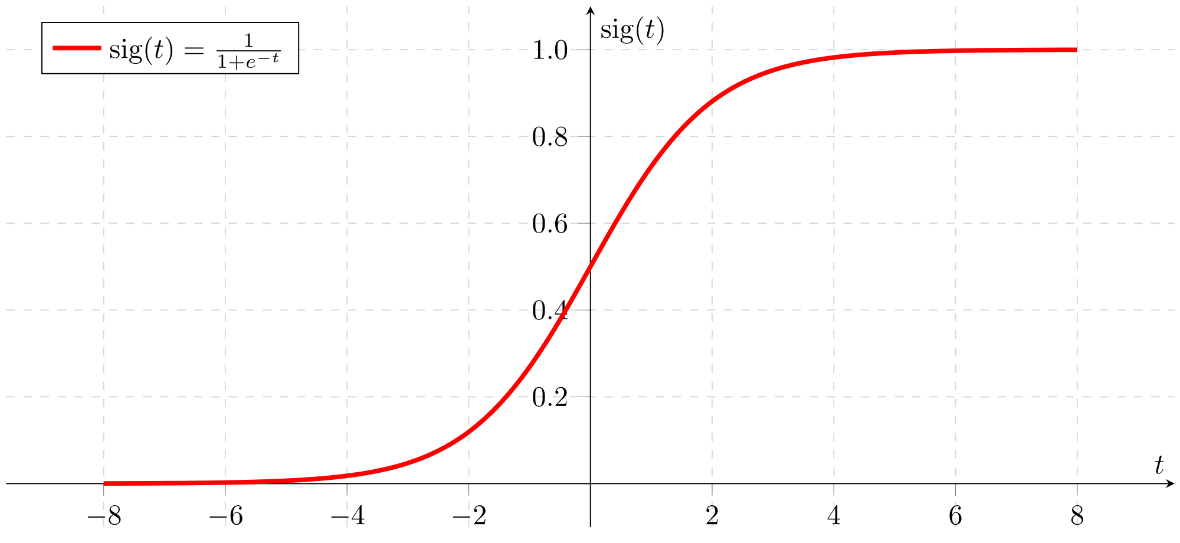
\includegraphics[width=0.8\textwidth]{course1/sigmoid}
\end{center}
\caption{$sigmoid(t) = \frac{{\rm{1}}}{{{\rm{1 + }}{e^{ - t}}}}$}
\end{figure}

To refer to a function belonging to a specific package you could call it using package\_name.function(). Run the code below to see an example with math.exp().

\begin{minted}{python}
# GRADED FUNCTION: basic_sigmoid
import math

def basic_sigmoid(x):
    """
    Compute sigmoid of x.

    Arguments:
    x -- A scalar

    Return:
    s -- sigmoid(x)
    """
    
    ### START CODE HERE ### (≈ 1 line of code)
    s = 1/(1+math.exp(-x))
    ### END CODE HERE ###
    
    return s
\end{minted}

Actually, we rarely use the ``math" library in deep learning because the inputs of the functions are real numbers. In deep learning we mostly use matrices and vectors. This is why numpy is more useful.

In fact, if $ x = (x_1, x_2, ..., x_n)$ is a row vector then $np.exp(x)$ will apply the exponential function to every element of x. The output will thus be: $np.exp(x) = (e^{x_1}, e^{x_2}, ..., e^{x_n})$
\begin{minted}{python}
import numpy as np

# example of np.exp
x = np.array([1, 2, 3])
print(np.exp(x)) # result is (exp(1), exp(2), exp(3))

#output
[  2.71828183   7.3890561   20.08553692]
\end{minted}

Furthermore, if x is a vector, then a Python operation such as $s = x + 3$ or $s = \frac{1}{x}$ will output s as a vector of the same size as x.
\begin{minted}{python}
# example of vector operation
x = np.array([1, 2, 3])
print (x + 3)

#output
[4 5 6]
\end{minted}

{\textbf {Exercise}}: Implement the sigmoid function using numpy. 

{\textbf {Instructions}}: x could now be either a real number, a vector, or a matrix. The data structures we use in numpy to represent these shapes (vectors, matrices...) are called numpy arrays. You don't need to know more for now.

For x $\in$ $\mathbb{R}^n$ ,
\begin{equation}
sigmoid(x) = sigmoid\begin{pmatrix}
    x_1  \\
    x_2  \\
    ...  \\
    x_n  \\
\end{pmatrix} = \begin{pmatrix}
    \frac{1}{1+e^{-x_1}}  \\
    \frac{1}{1+e^{-x_2}}  \\
    ...  \\
    \frac{1}{1+e^{-x_n}}  \\
\end{pmatrix}
\end{equation}

\begin{minted}{python}
# GRADED FUNCTION: sigmoid
import numpy as np # this means you can access numpy functions by writing np.function() instead of numpy.function()

def sigmoid(x):
    """
    Compute the sigmoid of x

    Arguments:
    x -- A scalar or numpy array of any size

    Return:
    s -- sigmoid(x)
    """
    
    ### START CODE HERE ### (≈ 1 line of code)
    s = 1/(1+np.exp(-x))
    ### END CODE HERE ###
    
    return s
\end{minted}

\begin{minted}{python}
x = np.array([1,2,3])
sigmoid(x)

#output
array([ 0.73105858,  0.88079708,  0.95257413])
\end{minted}

\subsubsubsection{Sigmoid gradient}

As you've seen in lecture, you will need to compute gradients to optimize loss functions using backpropagation. Let's code your first gradient function.

{\textbf {Exercise}}: Implement the function sigmoid\_grad() to compute the gradient of the sigmoid function with respect to its input x. The formula is: 
\begin{equation}
sigmoid\_derivative(x) = \sigma'(x) = \sigma(x) (1 - \sigma(x))
\end{equation}

You often code this function in two steps:
\begin{itemize}
\item[1.] Set s to be the sigmoid of x. You might find your sigmoid(x) function useful.
\item[2.] Compute $\sigma'(x) = s(1-s)$
\end{itemize}


\begin{minted}{python}
# GRADED FUNCTION: sigmoid_derivative
def sigmoid_derivative(x):
    """
    Compute the gradient (also called the slope or derivative) of the sigmoid function with respect to its input x.
    You can store the output of the sigmoid function into variables and then use it to calculate the gradient.
    
    Arguments:
    x -- A scalar or numpy array

    Return:
    ds -- Your computed gradient.
    """
    
    ### START CODE HERE ### (≈ 2 lines of code)
    s = 1/(1+np.exp(-x))
    ds = s*(1-s)
    ### END CODE HERE ###
    
    return ds
\end{minted}



\subsubsubsection{Reshaping arrays}
Two common numpy functions used in deep learning are \href{https://docs.scipy.org/doc/numpy/reference/generated/numpy.ndarray.shape.html}{np.shape} and \href{https://docs.scipy.org/doc/numpy/reference/generated/numpy.reshape.html}{np.reshape()}. 
\begin{itemize}
\item X.shape is used to get the shape (dimension) of a matrix/vector X. 
\item X.reshape(...) is used to reshape X into some other dimension. 
\end{itemize}

For example, in computer science, an image is represented by a 3D array of shape $(length, height, depth = 3)$. However, when you read an image as the input of an algorithm you convert it to a vector of shape $(length*height*3, 1)$. In other words, you ``unroll", or reshape, the 3D array into a 1D vector.

\begin{figure}[h]
\begin{center}
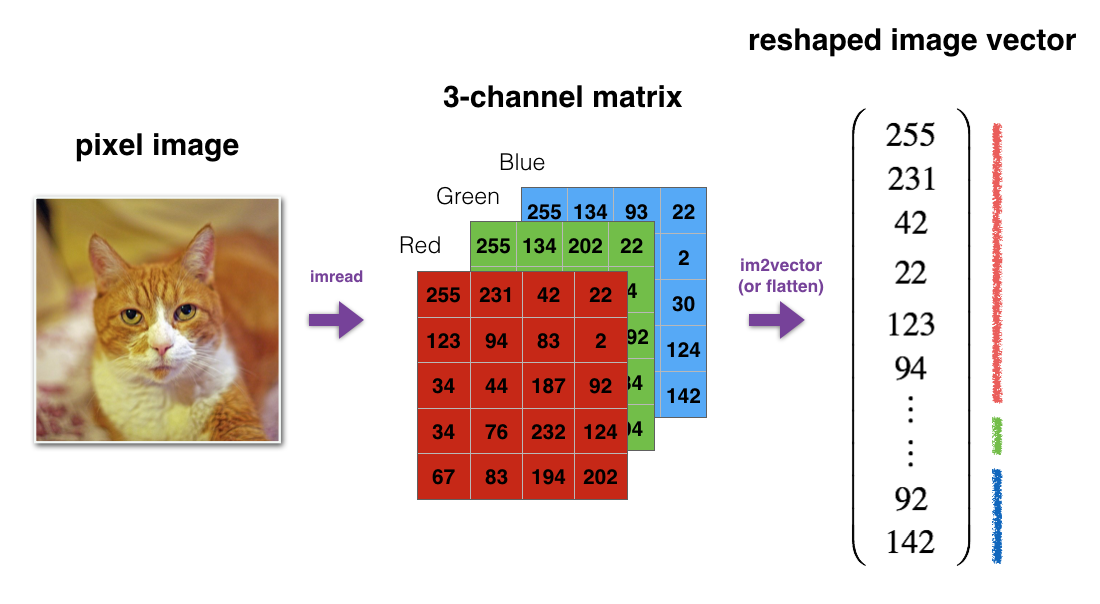
\includegraphics[width=0.8\textwidth]{course1/image2vector}
\end{center}
\caption{Reshape image a vector}
\end{figure}

{\textbf {Exercise}}: Implement ``image2vector()'' that takes an input of shape (length, height, 3) and returns a vector of shape (length\*height\*3, 1). For example, if you would like to reshape an array v of shape (a, b, c) into a vector of shape (a*b,c) you would do:
\begin{minted}{python}
v = v.reshape((v.shape[0]*v.shape[1], v.shape[2])) # v.shape[0] = a ; v.shape[1] = b ; v.shape[2] = c
\end{minted}

Please don't hardcode the dimensions of image as a constant. Instead look up the quantities you need with ``image.shape[0]'', etc. 

\begin{minted}{python}
# GRADED FUNCTION: image2vector
def image2vector(image):
    """
    Argument:
    image -- a numpy array of shape (length, height, depth)
    
    Returns:
    v -- a vector of shape (length*height*depth, 1)
    """
    
    ### START CODE HERE ### (≈ 1 line of code)
    v = image.reshape((image.shape[0]*image.shape[1]*image.shape[2]),1)
    ### END CODE HERE ###
    
    return v
\end{minted}


\subsubsubsection{Normalizing rows}

Another common technique we use in Machine Learning and Deep Learning is to normalize our data. It often leads to a better performance because gradient descent converges faster after normalization. Here, by normalization we mean changing x to $ \frac{x}{\| x\|} $ (dividing each row vector of x by its norm).

For example, if 
\begin{equation}
x = 
\begin{bmatrix}
    0 & 3 & 4 \\
    2 & 6 & 4 \\
\end{bmatrix}
\end{equation}
then 
\begin{equation}
\| x\| = np.linalg.norm(x, axis = 1, keepdims = True) = \begin{bmatrix}
    5 \\
    \sqrt{56} \\
\end{bmatrix}
\end{equation}
and
\begin{equation}
x\_normalized = \frac{x}{\| x\|} = \begin{bmatrix}
    0 & \frac{3}{5} & \frac{4}{5} \\
    \frac{2}{\sqrt{56}} & \frac{6}{\sqrt{56}} & \frac{4}{\sqrt{56}} \\
\end{bmatrix}
\end{equation}
Note that you can divide matrices of different sizes and it works fine: this is called broadcasting and you're going to learn about it in part \ref{Broadcasting}.

{\textbf {Exercise}}:  Implement normalizeRows() to normalize the rows of a matrix. After applying this function to an input matrix x, each row of x should be a vector of unit length (meaning length 1).

\begin{minted}{python}
# GRADED FUNCTION: normalizeRows
def normalizeRows(x):
    """
    Implement a function that normalizes each row of the matrix x (to have unit length).
    
    Argument:
    x -- A numpy matrix of shape (n, m)
    
    Returns:
    x -- The normalized (by row) numpy matrix. You are allowed to modify x.
    """
    
    ### START CODE HERE ### (≈ 2 lines of code)
    # Compute x_norm as the norm 2 of x. Use np.linalg.norm(..., ord = 2, axis = ..., keepdims = True)
    x_norm = np.linalg.norm(x,axis=1,keepdims=True)
    
    # Divide x by its norm.
    x = x/x_norm
    ### END CODE HERE ###

    return x
\end{minted}

\begin{minted}{python}
x = np.array([
    [0, 3, 4],
    [1, 6, 4]])
print("normalizeRows(x) = " + str(normalizeRows(x)))

#output
normalizeRows(x) = [[ 0.          0.6         0.8       ]
 [ 0.13736056  0.82416338  0.54944226]]
\end{minted}

{\textbf {Note}}: In normalizeRows(), you can try to print the shapes of x\_norm and x, and then rerun the assessment. You'll find out that they have different shapes. This is normal given that x\_norm takes the norm of each row of x. So x\_norm has the same number of rows but only 1 column. So how did it work when you divided x by x\_norm? This is called broadcasting and we'll talk about it now!



\subsubsubsection{Broadcasting and the softmax function}\label{Broadcasting}

A very important concept to understand in numpy is "broadcasting". It is very useful for performing mathematical operations between arrays of different shapes. For the full details on broadcasting, you can read the official \href{http://docs.scipy.org/doc/numpy/user/basics.broadcasting.html}{broadcasting documentation}.

{\textbf {Exercise}}: Implement a softmax function using numpy. You can think of softmax as a normalizing function used when your algorithm needs to classify two or more classes. You will learn more about softmax in the second course of this specialization.

{\textbf {Instructions}}:
\begin{itemize}
\item for  x $\in$ $\mathbb{R}^{1\times n}$ , 
\begin{equation}
\begin{aligned}
softmax(x) &= softmax(\begin{bmatrix}
    x_1  &&
    x_2 &&
    ...  &&
    x_n  
\end{bmatrix}) \\
&= \begin{bmatrix}
     \frac{e^{x_1}}{\sum_{j}e^{x_j}}  &&
    \frac{e^{x_2}}{\sum_{j}e^{x_j}}  &&
    ...  &&
    \frac{e^{x_n}}{\sum_{j}e^{x_j}} 
\end{bmatrix} 
\end{aligned}
\end{equation}
\item for a matrix $ x \in \mathbb{R}^{m \times n} $,  $x_{ij}$ maps to the element in the $i^{th}$ row and $j^{th}$ column of $x$, thus we have: 
\begin{equation}
\begin{aligned}
softmax(x) &= softmax\begin{bmatrix}
    x_{11} & x_{12} & x_{13} & \dots  & x_{1n} \\
    x_{21} & x_{22} & x_{23} & \dots  & x_{2n} \\
    \vdots & \vdots & \vdots & \ddots & \vdots \\
    x_{m1} & x_{m2} & x_{m3} & \dots  & x_{mn}
\end{bmatrix} \\
&= \begin{bmatrix}
    \frac{e^{x_{11}}}{\sum_{j}e^{x_{1j}}} & \frac{e^{x_{12}}}{\sum_{j}e^{x_{1j}}} & \frac{e^{x_{13}}}{\sum_{j}e^{x_{1j}}} & \dots  & \frac{e^{x_{1n}}}{\sum_{j}e^{x_{1j}}} \\
    \frac{e^{x_{21}}}{\sum_{j}e^{x_{2j}}} & \frac{e^{x_{22}}}{\sum_{j}e^{x_{2j}}} & \frac{e^{x_{23}}}{\sum_{j}e^{x_{2j}}} & \dots  & \frac{e^{x_{2n}}}{\sum_{j}e^{x_{2j}}} \\
    \vdots & \vdots & \vdots & \ddots & \vdots \\
    \frac{e^{x_{m1}}}{\sum_{j}e^{x_{mj}}} & \frac{e^{x_{m2}}}{\sum_{j}e^{x_{mj}}} & \frac{e^{x_{m3}}}{\sum_{j}e^{x_{mj}}} & \dots  & \frac{e^{x_{mn}}}{\sum_{j}e^{x_{mj}}}
\end{bmatrix} \\
&= \begin{pmatrix}
    softmax\text{(first row of x)}  \\
    softmax\text{(second row of x)} \\
    ...  \\
    softmax\text{(last row of x)} \\
\end{pmatrix}
\end{aligned}
\end{equation}
\end{itemize}


\begin{minted}{python}
# GRADED FUNCTION: softmax
def softmax(x):
    """Calculates the softmax for each row of the input x.

    Your code should work for a row vector and also for matrices of shape (n, m).

    Argument:
    x -- A numpy matrix of shape (n,m)

    Returns:
    s -- A numpy matrix equal to the softmax of x, of shape (n,m)
    """

    # Apply exp() element-wise to x. Use np.exp(...).
    x_exp = np.exp(x)

    # Create a vector x_sum that sums each row of x_exp. Use np.sum(..., axis = 1, keepdims = True).
    x_sum = np.sum(x_exp,axis = 1,keepdims = True)
    
    # Compute softmax(x) by dividing x_exp by x_sum. It should automatically use numpy broadcasting.
    s = x_exp/x_sum
    
    return s
\end{minted}

{\textbf {Note}}:

If you print the shapes of x\_exp, x\_sum and s above and rerun the assessment cell, you will see that x\_sum is of shape (2,1) while x\_exp and s are of shape (2,5). x\_exp/x\_sum works due to python broadcasting.

Congratulations! You now have a pretty good understanding of python numpy and have implemented a few useful functions that you will be using in deep learning.


{\textbf {What you need to remember:
\begin{itemize}
\item np.exp(x) works for any np.array x and applies the exponential function to every coordinate
\item the sigmoid function and its gradient
\item image2vector is commonly used in deep learning
\item np.reshape is widely used. In the future, you'll see that keeping your matrix/vector dimensions straight will go toward eliminating a lot of bugs.
\item numpy has efficient built-in functions
\item broadcasting is extremely useful
\end{itemize}
}}



\subsubsection{Vectorization}

In deep learning, you deal with very large datasets. Hence, a non-computationally-optimal function can become a huge bottleneck in your algorithm and can result in a model that takes ages to run. To make sure that your code is computationally efficient, you will use vectorization. For example, try to tell the difference between the following implementations of the dot/outer/elementwise product.
\begin{minted}{python}
import time

x1 = [9, 2, 5, 0, 0, 7, 5, 0, 0, 0, 9, 2, 5, 0, 0]
x2 = [9, 2, 2, 9, 0, 9, 2, 5, 0, 0, 9, 2, 5, 0, 0]

### CLASSIC DOT PRODUCT OF VECTORS IMPLEMENTATION ###
tic = time.process_time()
dot = 0
for i in range(len(x1)):
    dot+= x1[i]*x2[i]
toc = time.process_time()
print ("dot = " + str(dot) + "\n ----- Computation time = " + str(1000*(toc - tic)) + "ms")

### CLASSIC OUTER PRODUCT IMPLEMENTATION ###
tic = time.process_time()
outer = np.zeros((len(x1),len(x2))) # we create a len(x1)*len(x2) matrix with only zeros
for i in range(len(x1)):
    for j in range(len(x2)):
        outer[i,j] = x1[i]*x2[j]
toc = time.process_time()
print ("outer = " + str(outer) + "\n ----- Computation time = " + str(1000*(toc - tic)) + "ms")

### CLASSIC ELEMENTWISE IMPLEMENTATION ###
tic = time.process_time()
mul = np.zeros(len(x1))
for i in range(len(x1)):
    mul[i] = x1[i]*x2[i]
toc = time.process_time()
print ("elementwise multiplication = " + str(mul) + "\n ----- Computation time = " + str(1000*(toc - tic)) + "ms")

### CLASSIC GENERAL DOT PRODUCT IMPLEMENTATION ###
W = np.random.rand(3,len(x1)) # Random 3*len(x1) numpy array
tic = time.process_time()
gdot = np.zeros(W.shape[0])
for i in range(W.shape[0]):
    for j in range(len(x1)):
        gdot[i] += W[i,j]*x1[j]
toc = time.process_time()
print ("gdot = " + str(gdot) + "\n ----- Computation time = " + str(1000*(toc - tic)) + "ms")

\end{minted}

\begin{minted}{python}
#output
dot = 278
 ----- Computation time = 0.17511900000011238ms
 outer = [[ 81.  18.  18.  81.   0.  81.  18.  45.   0.   0.  81.  18.  45.   0.
    0.]
 [ 18.   4.   4.  18.   0.  18.   4.  10.   0.   0.  18.   4.  10.   0.
    0.]
 [ 45.  10.  10.  45.   0.  45.  10.  25.   0.   0.  45.  10.  25.   0.
    0.]
 [  0.   0.   0.   0.   0.   0.   0.   0.   0.   0.   0.   0.   0.   0.
    0.]
 [  0.   0.   0.   0.   0.   0.   0.   0.   0.   0.   0.   0.   0.   0.
    0.]
 [ 63.  14.  14.  63.   0.  63.  14.  35.   0.   0.  63.  14.  35.   0.
    0.]
 [ 45.  10.  10.  45.   0.  45.  10.  25.   0.   0.  45.  10.  25.   0.
    0.]
 [  0.   0.   0.   0.   0.   0.   0.   0.   0.   0.   0.   0.   0.   0.
    0.]
 [  0.   0.   0.   0.   0.   0.   0.   0.   0.   0.   0.   0.   0.   0.
    0.]
 [  0.   0.   0.   0.   0.   0.   0.   0.   0.   0.   0.   0.   0.   0.
    0.]
 [ 81.  18.  18.  81.   0.  81.  18.  45.   0.   0.  81.  18.  45.   0.
    0.]
 [ 18.   4.   4.  18.   0.  18.   4.  10.   0.   0.  18.   4.  10.   0.
    0.]
 [ 45.  10.  10.  45.   0.  45.  10.  25.   0.   0.  45.  10.  25.   0.
    0.]
 [  0.   0.   0.   0.   0.   0.   0.   0.   0.   0.   0.   0.   0.   0.
    0.]
 [  0.   0.   0.   0.   0.   0.   0.   0.   0.   0.   0.   0.   0.   0.
    0.]]
 ----- Computation time = 0.3380989999999251ms
elementwise multiplication = [ 81.   4.  10.   0.   0.  63.  10.   0.   0.   0.  81.   4.  25.   0.   0.]
 ----- Computation time = 0.1734490000000477ms
gdot = [ 25.22022143  27.33603654  20.18059712]
 ----- Computation time = 0.2346690000001317ms
\end{minted}




\begin{minted}{python}
x1 = [9, 2, 5, 0, 0, 7, 5, 0, 0, 0, 9, 2, 5, 0, 0]
x2 = [9, 2, 2, 9, 0, 9, 2, 5, 0, 0, 9, 2, 5, 0, 0]

### VECTORIZED DOT PRODUCT OF VECTORS ###
tic = time.process_time()
dot = np.dot(x1,x2)
toc = time.process_time()
print ("dot = " + str(dot) + "\n ----- Computation time = " + str(1000*(toc - tic)) + "ms")

### VECTORIZED OUTER PRODUCT ###
tic = time.process_time()
outer = np.outer(x1,x2)
toc = time.process_time()
print ("outer = " + str(outer) + "\n ----- Computation time = " + str(1000*(toc - tic)) + "ms")

### VECTORIZED ELEMENTWISE MULTIPLICATION ###
tic = time.process_time()
mul = np.multiply(x1,x2)
toc = time.process_time()
print ("elementwise multiplication = " + str(mul) + "\n ----- Computation time = " + str(1000*(toc - tic)) + "ms")

### VECTORIZED GENERAL DOT PRODUCT ###
tic = time.process_time()
dot = np.dot(W,x1)
toc = time.process_time()
print ("gdot = " + str(dot) + "\n ----- Computation time = " + str(1000*(toc - tic)) + "ms")
\end{minted}


\begin{minted}{python}
#output
dot = 278
 ----- Computation time = 0.1825449999999229ms
outer = [[81 18 18 81  0 81 18 45  0  0 81 18 45  0  0]
 [18  4  4 18  0 18  4 10  0  0 18  4 10  0  0]
 [45 10 10 45  0 45 10 25  0  0 45 10 25  0  0]
 [ 0  0  0  0  0  0  0  0  0  0  0  0  0  0  0]
 [ 0  0  0  0  0  0  0  0  0  0  0  0  0  0  0]
 [63 14 14 63  0 63 14 35  0  0 63 14 35  0  0]
 [45 10 10 45  0 45 10 25  0  0 45 10 25  0  0]
 [ 0  0  0  0  0  0  0  0  0  0  0  0  0  0  0]
 [ 0  0  0  0  0  0  0  0  0  0  0  0  0  0  0]
 [ 0  0  0  0  0  0  0  0  0  0  0  0  0  0  0]
 [81 18 18 81  0 81 18 45  0  0 81 18 45  0  0]
 [18  4  4 18  0 18  4 10  0  0 18  4 10  0  0]
 [45 10 10 45  0 45 10 25  0  0 45 10 25  0  0]
 [ 0  0  0  0  0  0  0  0  0  0  0  0  0  0  0]
 [ 0  0  0  0  0  0  0  0  0  0  0  0  0  0  0]]
 ----- Computation time = 0.15074200000020355ms
elementwise multiplication = [81  4 10  0  0 63 10  0  0  0 81  4 25  0  0]
 ----- Computation time = 0.13718599999990033ms
gdot = [ 25.22022143  27.33603654  20.18059712]
 ----- Computation time = 0.4201209999998845ms
\end{minted}

As you may have noticed, the vectorized implementation is much cleaner and more efficient. For bigger vectors/matrices, the differences in running time become even bigger.

{\textbf {Note}} that np.dot() performs a matrix-matrix or matrix-vector multiplication. This is different from np.multiply() and the * operator (which is equivalent to  .* in Matlab/Octave), which performs an element-wise multiplication.



\subsubsubsection{Implement the L1 and L2 loss functions}

{\textbf {Exercise}}: Implement the numpy vectorized version of the L1 loss. You may find the function abs(x) (absolute value of x) useful.

{\textbf {Reminder}}:
\begin{itemize}
\item The loss is used to evaluate the performance of your model. The bigger your loss is, the more different your predictions ($ \hat{y} $) are from the true values ($y$). In deep learning, you use optimization algorithms like Gradient Descent to train your model and to minimize the cost.
\item L1 loss is defined as:
\begin{equation}
 L_1(\hat{y}, y) = \sum_{i=0}^m|y^{(i)} - \hat{y}^{(i)}| 
\end{equation}
\end{itemize}
 
\begin{minted}{python} 
# GRADED FUNCTION: L1
def L1(yhat, y):
    """
    Arguments:
    yhat -- vector of size m (predicted labels)
    y -- vector of size m (true labels)
    
    Returns:
    loss -- the value of the L1 loss function defined above
    """
    
    loss = sum(abs(y-yhat))
    
    return loss
\end{minted} 

\begin{minted}{python} 
yhat = np.array([.9, 0.2, 0.1, .4, .9])
y = np.array([1, 0, 0, 1, 1])
print("L1 = " + str(L1(yhat,y))) 
\end{minted}  

{\textbf {Exercise}}: Implement the numpy vectorized version of the L2 loss. There are several way of implementing the L2 loss but you may find the function np.dot() useful. As a reminder, if $x = [x_1, x_2, ..., x_n]$, then ``np.dot(x,x)'' = $\sum_{j=0}^n x_j^{2}$. 

L2 loss is defined as 
\begin{equation}
L_2(\hat{y},y) = \sum_{i=0}^m(y^{(i)} - \hat{y}^{(i)})^2 
\end{equation}



\begin{minted}{python} 
# GRADED FUNCTION: L2
def L2(yhat, y):
    """
    Arguments:
    yhat -- vector of size m (predicted labels)
    y -- vector of size m (true labels)
    
    Returns:
    loss -- the value of the L2 loss function defined above
    """

    loss = np.dot(y-yhat,y-yhat)
    
    return loss
\end{minted}  
\vspace{-0.5cm}
\begin{minted}{python} 
yhat = np.array([.9, 0.2, 0.1, .4, .9])
y = np.array([1, 0, 0, 1, 1])
print("L2 = " + str(L2(yhat,y)))
\end{minted}  

\noindent{\textbf {What to remember:
\begin{itemize}
\item Vectorization is very important in deep learning. It provides computational efficiency and clarity.
\item You have reviewed the L1 and L2 loss.
\item You are familiar with many numpy functions such as np.sum, np.dot, np.multiply, np.maximum, etc...
\end{itemize}
}}


\clearpage


\subsection{Logistic Regression with a Neural Network mindset}

Welcome to the first (required) programming exercise of the deep learning specialization. In this notebook you will build your first image recognition algorithm. You will build a cat classifier that recognizes cats with 70\% accuracy!


\begin{figure}[h]
\begin{center}
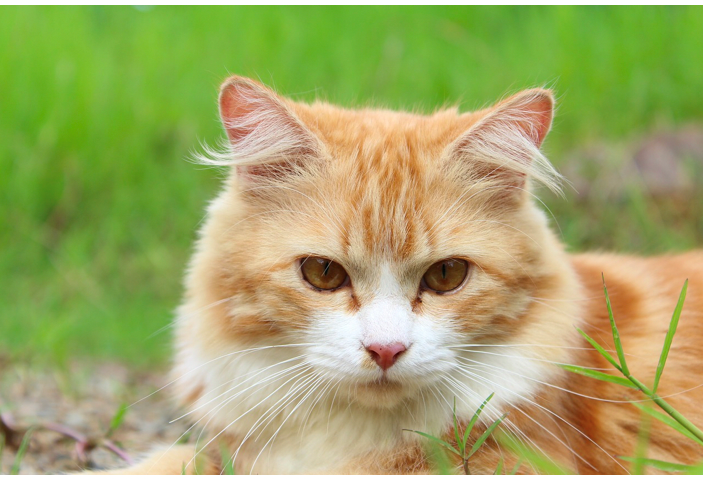
\includegraphics[width=0.5\textwidth]{course1/cat}
\end{center}
\caption{cat}
\label{fig:cat}
\end{figure}

As you keep learning new techniques you will increase it to 80+ \% accuracy on cat vs. non-cat datasets. By completing this assignment you will:
\begin{itemize}
\item  Work with logistic regression in a way that builds intuition relevant to neural networks.

\item  Learn how to minimize the cost function.

\item  Understand how derivatives of the cost are used to update parameters.
\end{itemize}

Take your time to complete this assignment and make sure you get the expected outputs when working through the different exercises. In some code blocks, you will find a "\#GRADED FUNCTION: functionName" comment. Please do not modify these comments. After you are done, submit your work and check your results. You need to score 70\% to pass. Good luck :) !


{\textbf {Instructions}}:
\begin{itemize}
\item  Do not use loops (for/while) in your code, unless the instructions explicitly ask you to do so.
\end{itemize}

{\textbf {You will learn to}}:
\begin{itemize}
\item Build the general architecture of a learning algorithm, including:
\begin{itemize}
\item Initializing parameters
\item Calculating the cost function and its gradient
\item Using an optimization algorithm (gradient descent)
\end{itemize}
\item Gather all three functions above into a main model function, in the right order.
\end{itemize}


\subsubsection{Packages}

First, let's run the cell below to import all the packages that you will need during this assignment. 
\begin{itemize}
\item \href{www.numpy.org}{numpy} is the fundamental package for scientific computing with Python.
\item \href{http://www.h5py.org}{h5py} is a common package to interact with a dataset that is stored on an H5 file.
\item \href{http://matplotlib.org}{matplotlib} is a famous library to plot graphs in Python.
\item \href{http://www.pythonware.com/products/pil/}{PIL} are used here to test your model with your own picture at the end.
\end{itemize}

\begin{mypython}
import numpy as np
import matplotlib.pyplot as plt
import h5py
import scipy
from PIL import Image
from scipy import ndimage
from lr_utils import load_dataset

#matplotlib inline
\end{mypython}





\subsubsection{Overview of the Problem set}

{\textbf {Problem Statement}}: You are given a dataset ("data.h5") containing:
\begin{itemize}
\item a training set of m\_train images labeled as cat (y=1) or non-cat (y=0)
\item a test set of m\_test images labeled as cat or non-cat
\item each image is of shape (num\_px, num\_px, 3) where 3 is for the 3 channels (RGB). Thus, each image is square (height = num\_px) and (width = num\_px).
\end{itemize}

You will build a simple image-recognition algorithm that can correctly classify pictures as cat or non-cat.

Let's get more familiar with the dataset. Load the data by running the following code.

\begin{minted}{python}
# Loading the data (cat/non-cat)
train_set_x_orig, train_set_y, test_set_x_orig, test_set_y, classes = load_dataset()
\end{minted}

We added "\_orig" at the end of image datasets (train and test) because we are going to preprocess them. After preprocessing, we will end up with train\_set\_x and test\_set\_x (the labels train\_set\_y and test\_set\_y don't need any preprocessing).\\
Each line of your train\_set\_x\_orig and test\_set\_x\_orig is an array representing an image. You can visualize an example by running the following code. Feel free also to change the index value and re-run to see other images.

\begin{minted}{python}
# Example of a picture
index = 25
plt.imshow(train_set_x_orig[index])
print ("y = " + str(train_set_y[:, index]) + ", it's a '" + classes[np.squeeze(train_set_y[:, index])].decode("utf-8") +  "' picture.")
\end{minted}

Many software bugs in deep learning come from having matrix/vector dimensions that don't fit. If you can keep your matrix/vector dimensions straight you will go a long way toward eliminating many bugs.

{\textbf {Exercise}: Find the values for:
\begin{itemize}
\item m\_train (number of training examples)
\item m\_test (number of test examples)
\item num\_px (= height = width of a training image)
\end{itemize}

Remember that train\_set\_x\_orig is a numpy-array of shape (m\_train, num\_px, num\_px, 3). For instance, you can access m\_train by writing train\_set\_x\_orig.shape[0].

\begin{minted}{python}
### START CODE HERE ### (≈ 3 lines of code)
m_train = train_set_x_orig.shape[0]
m_test = test_set_x_orig.shape[0]
num_px = train_set_x_orig.shape[1]
### END CODE HERE ###

print ("Number of training examples: m_train = " + str(m_train))
print ("Number of testing examples: m_test = " + str(m_test))
print ("Height/Width of each image: num_px = " + str(num_px))
print ("Each image is of size: (" + str(num_px) + ", " + str(num_px) + ", 3)")
print ("train_set_x shape: " + str(train_set_x_orig.shape))
print ("train_set_y shape: " + str(train_set_y.shape))
print ("test_set_x shape: " + str(test_set_x_orig.shape))
print ("test_set_y shape: " + str(test_set_y.shape))
\end{minted}

Output for m\_train, m\_test and num\_px:
\begin{minted}{python}
Number of training examples: m_train = 209
Number of testing examples: m_test = 50
Height/Width of each image: num_px = 64
Each image is of size: (64, 64, 3)
train_set_x shape: (209, 64, 64, 3)
train_set_y shape: (1, 209)
test_set_x shape: (50, 64, 64, 3)
test_set_y shape: (1, 50)
\end{minted}


For convenience, you should now reshape images of shape (num\_px, num\_px, 3) in a numpy-array of shape (num\_px*num\_px*3, 1). After this, our training (and test) dataset is a numpy-array where each column represents a flattened image. There should be m\_train (respectively m\_test) columns.

{\textbf {Exercise}: Reshape the training and test data sets so that images of size (num\_px, num\_px, 3) are flattened into single vectors of shape  (num\_px*num\_px*3, 1).


A trick when you want to flatten a matrix X of shape (a,b,c,d) to a matrix X\_flatten of shape (b * c *d, a) is to use:
\begin{minted}{python}
X_flatten = X.reshape(-1,X.shape[0]) 
\end{minted}

\begin{minted}{python}
# Reshape the training and test examples

### START CODE HERE ### (≈ 2 lines of code)
train_set_x_flatten = train_set_x_orig.reshape(train_set_x_orig.shape[0],-1).T
test_set_x_flatten = test_set_x_orig.reshape(test_set_x_orig.shape[0],-1).T
### END CODE HERE ###

print ("train_set_x_flatten shape: " + str(train_set_x_flatten.shape))
print ("train_set_y shape: " + str(train_set_y.shape))
print ("test_set_x_flatten shape: " + str(test_set_x_flatten.shape))
print ("test_set_y shape: " + str(test_set_y.shape))
print ("sanity check after reshaping: " + str(train_set_x_flatten[0:5,0]))
\end{minted}

Output for train\_set\_x\_flatten shape, test\_set\_x\_flatten shape:
\begin{minted}{python}
train_set_x_flatten shape: (12288, 209)
train_set_y shape: (1, 209)
test_set_x_flatten shape: (12288, 50)
test_set_y shape: (1, 50)
sanity check after reshaping: [17 31 56 22 33]
\end{minted}

To represent color images, the red, green and blue channels (RGB) must be specified for each pixel, and so the pixel value is actually a vector of three numbers ranging from 0 to 255.

One common preprocessing step in machine learning is to center and standardize your dataset, meaning that you substract the mean of the whole numpy array from each example, and then divide each example by the standard deviation of the whole numpy array. But for picture datasets, it is simpler and more convenient and works almost as well to just divide every row of the dataset by 255 (the maximum value of a pixel channel).

Let's standardize our dataset.

\begin{minted}{python}
train_set_x = train_set_x_flatten/255.
test_set_x = test_set_x_flatten/255.
\end{minted}

{\color{blue}
{\textbf {What you need to remember}}:
 
Common steps for pre-processing a new dataset are:
\begin{itemize}
\item Figure out the dimensions and shapes of the problem (m\_train, m\_test, num\_px, ...)
\item Reshape the datasets such that each example is now a vector of size (num\_px * num\_px * 3, 1)
\item "Standardize" the data
\end{itemize}
}




\subsubsection{General Architecture of the learning algorithm}

\indent It's time to design a simple algorithm to distinguish cat images from non-cat images.

You will build a Logistic Regression, using a Neural Network mindset. The following Figure explains why {\textbf {Logistic Regression is actually a very simple Neural Network}}!

\begin{figure}[h]
\begin{center}
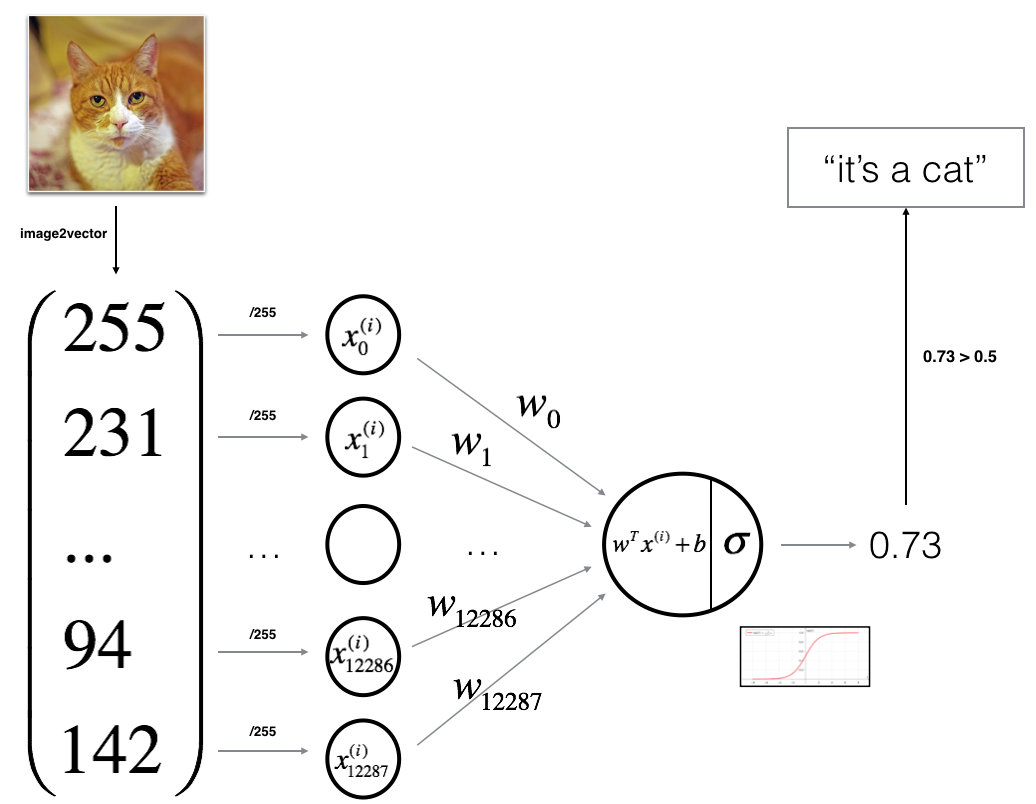
\includegraphics[width=0.7\textwidth]{course1/LogReg}
\end{center}
\caption{Principle of Logistic Regression }
\label{fig:LogReg}
\end{figure}


{\textbf {Mathematical expression of the algorithm}}:

For one example $x^{(i)}$:
\begin{align}
z^{(i)} &= w^T x^{(i)} + b \\
\hat{y}^{(i)} &= a^{(i)} = sigmoid(z^{(i)})\\
\mathcal{L}(a^{(i)}, y^{(i)}) &=  - y^{(i)}  \log(a^{(i)}) - (1-y^{(i)} )  \log(1-a^{(i)})
\end{align}


The cost is then computed by summing over all training examples:
\begin{align}
J = \frac{1}{m} \sum_{i=1}^m \mathcal{L}(a^{(i)}, y^{(i)})
\end{align}

{\textbf {Key steps}}: In this exercise, you will carry out the following steps:
\begin{itemize}
\item Initialize the parameters of the model
\item Learn the parameters for the model by minimizing the cost  
\item Use the learned parameters to make predictions (on the test set)
\item Analyse the results and conclude
\end{itemize}



\subsubsection{Building the parts of our algorithm}

The main steps for building a Neural Network are:
\begin{itemize}
\item Define the model structure (such as number of input features)
\item Initialize the model's parameters
\item Loop:
\begin{itemize}
\item Calculate current loss (forward propagation)
\item Calculate current gradient (backward propagation)
\item Update parameters (gradient descent)
\end{itemize}
\end{itemize}
You often build 1-3 separately and integrate them into one function we call model().


\subsubsubsection{Helper functions}

{\textbf {Exercise}}: Using your code from "Python Basics", implement sigmoid(). As you've seen in the figure above, you need to compute $sigmoid( w^T x + b) = \frac{1}{1 + e^{-(w^T x + b)}}$ to make predictions. Use np.exp().

\begin{mypython}
# GRADED FUNCTION: sigmoid

def sigmoid(z):
    """
    Compute the sigmoid of z

    Arguments:
    z -- A scalar or numpy array of any size.

    Return:
    s -- sigmoid(z)
    """

    ### START CODE HERE ### (≈ 1 line of code)
    s = 1/(1+np.exp(-z))
    ### END CODE HERE ###
    
    return s
\end{mypython}



\subsubsubsection{Initializing parameters}

{\textbf {Exercise}}: Implement parameter initialization in the cell below. You have to initialize w as a vector of zeros. If you don't know what numpy function to use, look up np.zeros() in the Numpy library's documentation.
\begin{mypython}
def initialize_with_zeros(dim):
    """
    This function creates a vector of zeros of shape (dim, 1) for w and initializes b to 0.
    
    Argument:
    dim -- size of the w vector we want (or number of parameters in this case)
    
    Returns:
    w -- initialized vector of shape (dim, 1)
    b -- initialized scalar (corresponds to the bias)
    """
    
    ### START CODE HERE ### (≈ 1 line of code)
    w = np.zeros((dim,1))
    b = 0
    ### END CODE HERE ###

    assert(w.shape == (dim, 1))
    assert(isinstance(b, float) or isinstance(b, int))
    
    return w, b
\end{mypython}

For image inputs, w will be of shape (num\_px  $\times$  num\_px  $\times$  3, 1).


\subsubsubsection{Forward and Backward propagation}

Now that your parameters are initialized, you can do the "forward" and "backward" propagation steps for learning the parameters.

{\textbf {Exercise}}: Implement a function propagate() that computes the cost function and its gradient.

{\textbf {Hints}}:

Forward Propagation:
\begin{itemize}
\item You get X
\item You compute $A = \sigma(w^T X + b) = (a^{(0)}, a^{(1)}, ..., a^{(m-1)}, a^{(m)})$
\item You calculate the cost function: $J = -\frac{1}{m}\sum_{i=1}^{m}y^{(i)}\log(a^{(i)})+(1-y^{(i)})\log(1-a^{(i)})$
\end{itemize}

Here are the two formulas you will be using: 
\begin{align}
\frac{\partial J}{\partial w} &= \frac{1}{m}X(A-Y)^T\\
\frac{\partial J}{\partial b} &= \frac{1}{m} \sum_{i=1}^m (a^{(i)}-y^{(i)})
\end{align}

Code is as follows:
\clearpage
\begin{mypython}
# GRADED FUNCTION: propagate

def propagate(w, b, X, Y):
    """
    Implement the cost function and its gradient for the propagation explained above

    Arguments:
    w -- weights, a numpy array of size (num_px * num_px * 3, 1)
    b -- bias, a scalar
    X -- data of size (num_px * num_px * 3, number of examples)
    Y -- true "label" vector (containing 0 if non-cat, 1 if cat) of size (1, number of examples)

    Return:
    cost -- negative log-likelihood cost for logistic regression
    dw -- gradient of the loss with respect to w, thus same shape as w
    db -- gradient of the loss with respect to b, thus same shape as b
    
    Tips:
    - Write your code step by step for the propagation. np.log(), np.dot()
    """
    
    m = X.shape[1]
    
    # FORWARD PROPAGATION (FROM X TO COST)
    ### START CODE HERE ### (≈ 2 lines of code)
    A =  sigmoid(np.dot(w.T,X)+b)    # compute activation
    cost =  -(np.dot(Y,np.log(A.T))+np.dot(np.log(1-A),(1-Y).T))/m  # compute cost
    ### END CODE HERE ###
    
    # BACKWARD PROPAGATION (TO FIND GRAD)
    ### START CODE HERE ### (≈ 2 lines of code)
    dw = np.dot(X,(A-Y).T)/m
    db = np.sum(A-Y)/m
    ### END CODE HERE ###

    assert(dw.shape == w.shape)
    assert(db.dtype == float)
    cost = np.squeeze(cost)
    assert(cost.shape == ())
    
    grads = {"dw": dw,
             "db": db}
    
    return grads, cost
\end{mypython}



\subsubsubsection{Optimization}
\begin{itemize}
\item You have initialized your parameters.
\item You are also able to compute a cost function and its gradient.
\item Now, you want to update the parameters using gradient descent.
\end{itemize}

{\textbf {Exercise}}: Write down the optimization function. The goal is to learn $w$ and $b$ by minimizing the cost function $J$. For a parameter $\theta$, the update rule is $ \theta = \theta - \alpha \text{ } d\theta$, where $\alpha$ is the learning rate.

\begin{minted}{python}
# GRADED FUNCTION: optimize

def optimize(w, b, X, Y, num_iterations, learning_rate, print_cost = False):
    """
    This function optimizes w and b by running a gradient descent algorithm
    
    Arguments:
    w -- weights, a numpy array of size (num_px * num_px * 3, 1)
    b -- bias, a scalar
    X -- data of shape (num_px * num_px * 3, number of examples)
    Y -- true "label" vector (containing 0 if non-cat, 1 if cat), of shape (1, number of examples)
    num_iterations -- number of iterations of the optimization loop
    learning_rate -- learning rate of the gradient descent update rule
    print_cost -- True to print the loss every 100 steps
    
    Returns:
    params -- dictionary containing the weights w and bias b
    grads -- dictionary containing the gradients of the weights and bias with respect to the cost function
    costs -- list of all the costs computed during the optimization, this will be used to plot the learning curve.
    
    Tips:
    You basically need to write down two steps and iterate through them:
        1) Calculate the cost and the gradient for the current parameters. Use propagate().
        2) Update the parameters using gradient descent rule for w and b.
    """
    
    costs = []
    
    for i in range(num_iterations):
        
        
        # Cost and gradient calculation (≈ 1-4 lines of code)
        ### START CODE HERE ### 
        grads, cost = propagate(w, b, X, Y)
        ### END CODE HERE ###
        
        # Retrieve derivatives from grads
        dw = grads["dw"]
        db = grads["db"]
        
        # update rule (≈ 2 lines of code)
        ### START CODE HERE ###
        w = w-learning_rate*dw
        b = b-learning_rate*db
        ### END CODE HERE ###
        
        # Record the costs
        if i % 100 == 0:
            costs.append(cost)
        
        # Print the cost every 100 training examples
        if print_cost and i % 100 == 0:
            print ("Cost after iteration %i: %f" %(i, cost))
    
    params = {"w": w,
              "b": b}
    
    grads = {"dw": dw,
             "db": db}
    
    return params, grads, costs
\end{minted}


\begin{minted}{python}
w, b, X, Y = np.array([[1.],[2.]]), 2., np.array([[1.,2.,-1.],[3.,4.,-3.2]]), np.array([[1,0,1]])
params, grads, costs = optimize(w, b, X, Y, num_iterations= 100, learning_rate = 0.009, print_cost = False)
print ("w = " + str(params["w"]))
print ("b = " + str(params["b"]))
print ("dw = " + str(grads["dw"]))
print ("db = " + str(grads["db"]))

#output
w = [[ 0.19033591]
 [ 0.12259159]]
b = 1.92535983008
dw = [[ 0.67752042]
 [ 1.41625495]]
db = 0.219194504541
\end{minted}



{\textbf {Exercise}}: The previous function will output the learned w and b. We are able to use w and b to predict the labels for a dataset X. Implement the predict() function. There is two steps to computing predictions:
\begin{itemize}
\item Calculate $\hat{Y} = A = \sigma(w^T X + b)$

\item Convert the entries of a into 0 (if activation <= 0.5) or 1 (if activation > 0.5), stores the predictions in a vector `Y\_prediction'. If you wish, you can use an `if'/`else' statement in a `for' loop (though there is also a way to vectorize this). 
\end{itemize}

\begin{mypython}
def predict(w, b, X):
    '''
    Predict whether the label is 0 or 1 using learned logistic regression parameters (w, b)
    
    Arguments:
    w -- weights, a numpy array of size (num_px * num_px * 3, 1)
    b -- bias, a scalar
    X -- data of size (num_px * num_px * 3, number of examples)
    
    Returns:
    Y_prediction -- a numpy array (vector) containing all predictions (0/1) for the examples in X
    '''
    
    m = X.shape[1]
    Y_prediction = np.zeros((1,m))
    w = w.reshape(X.shape[0], 1)
    
    # Compute vector "A" predicting the probabilities of a cat being present in the picture
    ### START CODE HERE ### (≈ 1 line of code)
    A = sigmoid(np.dot(w.T,X)+b)
    ### END CODE HERE ###
    
    for i in range(A.shape[1]):
        
        # Convert probabilities A[0,i] to actual predictions p[0,i]
        ### START CODE HERE ### (≈ 4 lines of code)
        if A[0][i]<=0.5:A[0][i]=0
        else: A[0][i]=1
    Y_prediction=A
        ### END CODE HERE ###
    
    assert(Y_prediction.shape == (1, m))
    
    return Y_prediction
\end{mypython}

{\color{blue}\textbf{
What to remember: You've implemented several functions that:
\begin{itemize}
\item Initialize (w,b)
\item Optimize the loss iteratively to learn parameters (w,b):
\begin{itemize}
\item computing the cost and its gradient
\item updating the parameters using gradient descent
\end{itemize}
\item Use the learned (w,b) to predict the labels for a given set of examples
\end{itemize}
}}



\subsubsection{Merge all functions into a model}\label{sec:logistic_regression}

You will now see how the overall model is structured by putting together all the building blocks (functions implemented in the previous parts) together, in the right order.

{\textbf {Exercise}}: Implement the model function. Use the following notation:
\begin{itemize}
\item  Y\_prediction for your predictions on the test set
\item  Y\_prediction\_train for your predictions on the train set
\item  w, costs, grads for the outputs of optimize()
\end{itemize}

Code is as follows:
\begin{minted}{python}
# GRADED FUNCTION: model

def model(X_train, Y_train, X_test, Y_test, num_iterations = 2000, learning_rate = 0.5, print_cost = False):
    """
    Builds the logistic regression model by calling the function you've implemented previously
    
    Arguments:
    X_train -- training set represented by a numpy array of shape (num_px * num_px * 3, m_train)
    Y_train -- training labels represented by a numpy array (vector) of shape (1, m_train)
    X_test -- test set represented by a numpy array of shape (num_px * num_px * 3, m_test)
    Y_test -- test labels represented by a numpy array (vector) of shape (1, m_test)
    num_iterations -- hyperparameter representing the number of iterations to optimize the parameters
    learning_rate -- hyperparameter representing the learning rate used in the update rule of optimize()
    print_cost -- Set to true to print the cost every 100 iterations
    
    Returns:
    d -- dictionary containing information about the model.
    """
    
    ### START CODE HERE ###
    
    # initialize parameters with zeros (≈ 1 line of code)
    w, b = initialize_with_zeros(X_train.shape[0])

    # Gradient descent (≈ 1 line of code)
    parameters, grads, costs = optimize(w, b, X_train, Y_train, num_iterations, learning_rate, print_cost)
    
    # Retrieve parameters w and b from dictionary "parameters"
    w = parameters["w"]
    b = parameters["b"]
    
    # Predict test/train set examples (≈ 2 lines of code)
    Y_prediction_test = predict(w, b, X_test)
    Y_prediction_train = predict(w, b, X_train)

    ### END CODE HERE ###

    # Print train/test Errors
    print("train accuracy: {} %".format(100 - np.mean(np.abs(Y_prediction_train - Y_train)) * 100))
    print("test accuracy: {} %".format(100 - np.mean(np.abs(Y_prediction_test - Y_test)) * 100))

    
    d = {"costs": costs,
         "Y_prediction_test": Y_prediction_test, 
         "Y_prediction_train" : Y_prediction_train, 
         "w" : w, 
         "b" : b,
         "learning_rate" : learning_rate,
         "num_iterations": num_iterations}
    
    return d
\end{minted}   
    
    
Run the following cell to train your model.
\begin{minted}{python}
d = model(train_set_x, train_set_y, test_set_x, test_set_y, num_iterations = 2000, learning_rate = 0.005, print_cost = True)

#Output:

Cost after iteration 0: 0.693147
Cost after iteration 100: 0.584508
Cost after iteration 200: 0.466949
Cost after iteration 300: 0.376007
Cost after iteration 400: 0.331463
Cost after iteration 500: 0.303273
Cost after iteration 600: 0.279880
Cost after iteration 700: 0.260042
Cost after iteration 800: 0.242941
Cost after iteration 900: 0.228004
Cost after iteration 1000: 0.214820
Cost after iteration 1100: 0.203078
Cost after iteration 1200: 0.192544
Cost after iteration 1300: 0.183033
Cost after iteration 1400: 0.174399
Cost after iteration 1500: 0.166521
Cost after iteration 1600: 0.159305
Cost after iteration 1700: 0.152667
Cost after iteration 1800: 0.146542
Cost after iteration 1900: 0.140872
train accuracy: 99.04306220095694 %
test accuracy: 70.0 %
\end{minted}


{\textbf {Comment}}: Training accuracy is close to 100\%. This is a good sanity check: your model is working and has high enough capacity to fit the training data. Test error is 68\%. It is actually not bad for this simple model, given the small dataset we used and that logistic regression is a linear classifier. But no worries, you'll build an even better classifier next week!

Also, you see that the model is clearly overfitting the training data. Later in this specialization you will learn how to reduce overfitting, for example by using regularization. Using the code below (and changing the index variable) you can look at predictions on pictures of the test set.


Let's also plot the cost function and the gradients.
\begin{mypython}
# Plot learning curve (with costs)
costs = np.squeeze(d['costs'])
plt.plot(costs)
plt.ylabel('cost')
plt.xlabel('iterations (per hundreds)')
plt.title("Learning rate =" + str(d["learning_rate"]))
plt.show()
\end{mypython}

\begin{figure}[h]
\begin{center}
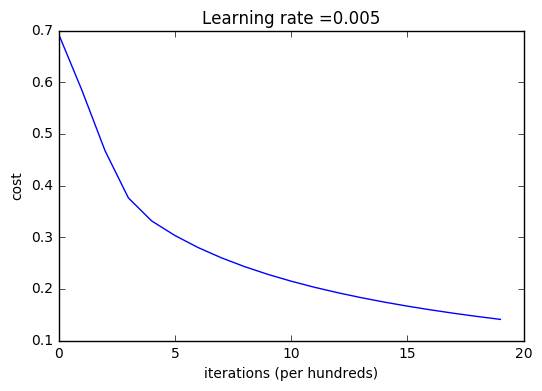
\includegraphics[width=0.7\textwidth]{course1/cost_curve}
\end{center}
\caption{cost function}
\label{fig:cost_function}
\end{figure}


{\textbf {Interpretation}}: You can see the cost decreasing. It shows that the parameters are being learned. However, you see that you could train the model even more on the training set. Try to increase the number of iterations in the cell above and rerun the cells. You might see that the training set accuracy goes up, but the test set accuracy goes down. This is called {\textbf {overfitting.}}

\begin{minted}{python}
d = model(train_set_x, train_set_y, test_set_x, test_set_y, num_iterations = 2500, learning_rate = 0.005, print_cost = True)

#Output:

train accuracy: 99.52153110047847 %
test accuracy: 68.0 %
\end{minted}



\subsubsection{Further analysis (optional/ungraded exercise)}

Congratulations on building your first image classification model. Let's analyze it further, and examine possible choices for the learning rate $\alpha$. 


{\textbf {Choice of learning rate}}

{\textbf {Reminder}}: In order for Gradient Descent to work you must choose the learning rate wisely. The learning rate $\alpha$ determines how rapidly we update the parameters. If the learning rate is too large we may "overshoot" the optimal value. Similarly, if it is too small we will need too many iterations to converge to the best values. That's why it is crucial to use a well-tuned learning rate.

Let's compare the learning curve of our model with several choices of learning rates. Run the cell below. This should take about 1 minute. Feel free also to try different values than the three we have initialized the learning\_rates variable to contain, and see what happens.

\begin{mypython}
learning_rates = [0.01, 0.001, 0.0001]
models = {}
for i in learning_rates:
    print ("learning rate is: " + str(i))
    models[str(i)] = model(train_set_x, train_set_y, test_set_x, test_set_y, num_iterations = 1500, learning_rate = i, print_cost = False)
    print ('\n' + "----------------------------------" + '\n')

for i in learning_rates:
    plt.plot(np.squeeze(models[str(i)]["costs"]), label= str(models[str(i)]["learning_rate"]))

plt.ylabel('cost')
plt.xlabel('iterations')

legend = plt.legend(loc='upper center', shadow=True)
frame = legend.get_frame()
frame.set_facecolor('0.90')
plt.show()
\end{mypython}


The result:
\begin{minted}{python}
learning rate is: 0.01
train accuracy: 99.52153110047847 %
test accuracy: 68.0 %

--------------------------------------

learning rate is: 0.001
train accuracy: 88.99521531100478 %
test accuracy: 64.0 %

--------------------------------------

learning rate is: 0.0001
train accuracy: 68.42105263157895 %
test accuracy: 36.0 %

--------------------------------------
\end{minted}

\begin{figure}[h]
\begin{center}
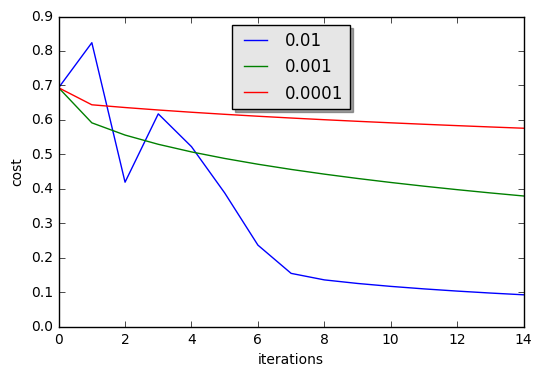
\includegraphics[width=0.7\textwidth]{course1/three_learning_rates}
\end{center}
\caption{compare the learning curve of model with three learning rates}
\label{three_learning_rates}
\end{figure}

{\color{red}\textbf {Interpretation}}:
\begin{itemize}
\item Different learning rates give different costs and thus different predictions results.
\item If the learning rate is too large (0.01), the cost may oscillate up and down. It may even diverge (though in this example, using 0.01 still eventually ends up at a good value for the cost).
\item A lower cost doesn't mean a better model. You have to check if there is possibly overfitting. It happens when the training accuracy is a lot higher than the test accuracy.
\item In deep learning, we usually recommend that you:
\begin{itemize}
\item Choose the learning rate that better minimizes the cost function.
\item If your model overfits, use other techniques to reduce overfitting. (We'll talk about this in later videos.)
\end{itemize}
\end{itemize}
}

\subsubsection{Test with your own image (optional/ungraded exercise)}
Congratulations on finishing this assignment. You can use your own image and see the output of your model. To do that:

1. Click on "File" in the upper bar of this notebook, then click "Open" to go on your Coursera Hub.

2. Add your image to this Jupyter Notebook's directory, in the "images" folder

3. Change your image's name in the following code

4. Run the code and check if the algorithm is right (1 = cat, 0 = non-cat)!


\begin{mypython}
my_image = "test2.jpg"   # change this to the name of your image file 

# We preprocess the image to fit your algorithm.
fname = "images/" + my_image
image = np.array(ndimage.imread(fname, flatten=False))
my_image = scipy.misc.imresize(image, size=(num_px,num_px)).reshape((1, num_px*num_px*3)).T
my_predicted_image = predict(d["w"], d["b"], my_image)

plt.imshow(image)
print("y = " + str(np.squeeze(my_predicted_image)) + ", your algorithm predicts a \"" + classes[int(np.squeeze(my_predicted_image)),].decode("utf-8") +  "\" picture.")
\end{mypython}


{\color{red}\textbf {What to remember from this assignment}}:

1. Preprocessing the dataset is important.

2. You implemented each function separately: initialize(), propagate(), optimize(). Then you built a model().

3. Tuning the learning rate (which is an example of a "hyperparameter") can make a big difference to the algorithm. You will see more examples of this later in this course!
}


\clearpage


\subsubsection{Code of Logistic Regression with a Neural Network}
\begin{minted}{python}

#Logistic Regression with a Neural Network mindset

# -*- coding: utf-8 -*-

import numpy as np
import matplotlib.pyplot as plt
import h5py
import scipy
from PIL import Image
from scipy import ndimage
from lr_utils import load_dataset

# Loading the data (cat/non-cat)
train_set_x_orig, train_set_y, test_set_x_orig, test_set_y, classes = load_dataset()


m_train = train_set_x_orig.shape[0]
m_test = test_set_x_orig.shape[0]
num_px = train_set_x_orig.shape[1]

# Reshape the training and test examples
train_set_x_flatten = train_set_x_orig.reshape(train_set_x_orig.shape[0],-1).T
test_set_x_flatten = test_set_x_orig.reshape(test_set_x_orig.shape[0],-1).T

#"Standardize" the data
train_set_x = train_set_x_flatten/255.
test_set_x = test_set_x_flatten/255.


# GRADED FUNCTION: sigmoid
def sigmoid(x):
    """
    Compute the sigmoid of x

    Arguments:
    x -- A scalar or numpy array of any size

    Return:
    s -- sigmoid(x)
    """

    s = 1/(1+np.exp(-x))
    
    return s


# GRADED FUNCTION: initialize_with_zeros
def initialize_with_zeros(dim):
    """
    This function creates a vector of zeros of shape (dim, 1) for w and initializes b to 0.
    
    Argument:
    dim -- size of the w vector we want (or number of parameters in this case)
    
    Returns:
    w -- initialized vector of shape (dim, 1)
    b -- initialized scalar (corresponds to the bias)
    """

    w = np.zeros((dim,1))
    b = 0

    assert(w.shape == (dim, 1))
    assert(isinstance(b, float) or isinstance(b, int))
    
    return w, b


# GRADED FUNCTION: propagate
def propagate(w, b, X, Y):
    """
    Implement the cost function and its gradient for the propagation explained above

    Arguments:
    w -- weights, a numpy array of size (num_px * num_px * 3, 1)
    b -- bias, a scalar
    X -- data of size (num_px * num_px * 3, number of examples)
    Y -- true "label" vector (containing 0 if non-cat, 1 if cat) of size (1, number of examples)

    Return:
    cost -- negative log-likelihood cost for logistic regression
    dw -- gradient of the loss with respect to w, thus same shape as w
    db -- gradient of the loss with respect to b, thus same shape as b
    
    Tips:
    - Write your code step by step for the propagation. np.log(), np.dot()
    """
    
    m = X.shape[1]
    
    # FORWARD PROPAGATION (FROM X TO COST)
    A =  sigmoid(np.dot(w.T,X)+b)    # compute activation
    cost =  -(np.dot(Y,np.log(A.T))+np.dot(np.log(1-A),(1-Y).T))/m  # compute cost
    
    # BACKWARD PROPAGATION (TO FIND GRAD)
    dw = np.dot(X,(A-Y).T)/m
    db = np.sum(A-Y)/m

    assert(dw.shape == w.shape)
    assert(db.dtype == float)
    cost = np.squeeze(cost)
    assert(cost.shape == ())
    
    grads = {"dw": dw,
             "db": db}
    
    return grads, cost

# GRADED FUNCTION: optimize
def optimize(w, b, X, Y, num_iterations, learning_rate, print_cost = False):
    """
    This function optimizes w and b by running a gradient descent algorithm
    
    Arguments:
    w -- weights, a numpy array of size (num_px * num_px * 3, 1)
    b -- bias, a scalar
    X -- data of shape (num_px * num_px * 3, number of examples)
    Y -- true "label" vector (containing 0 if non-cat, 1 if cat), of shape (1, number of examples)
    num_iterations -- number of iterations of the optimization loop
    learning_rate -- learning rate of the gradient descent update rule
    print_cost -- True to print the loss every 100 steps
    
    Returns:
    params -- dictionary containing the weights w and bias b
    grads -- dictionary containing the gradients of the weights and bias with respect to the cost function
    costs -- list of all the costs computed during the optimization, this will be used to plot the learning curve.
    
    Tips:
    You basically need to write down two steps and iterate through them:
        1) Calculate the cost and the gradient for the current parameters. Use propagate().
        2) Update the parameters using gradient descent rule for w and b.
    """
    
    costs = []
    
    for i in range(num_iterations):
        
        
        # Cost and gradient calculation (≈ 1-4 lines of code)
        grads, cost = propagate(w, b, X, Y)
        
        # Retrieve derivatives from grads
        dw = grads["dw"]
        db = grads["db"]
        
        # update rule
        w = w-learning_rate*dw
        b = b-learning_rate*db
        
        # Record the costs
        if i % 100 == 0:
            costs.append(cost)
        
        # Print the cost every 100 training examples
        if print_cost and i % 100 == 0:
            print ("Cost after iteration %i: %f" %(i, cost))
    
    params = {"w": w,
              "b": b}
    
    grads = {"dw": dw,
             "db": db}
    
    return params, grads, costs


# GRADED FUNCTION: predict
def predict(w, b, X):
    '''
    Predict whether the label is 0 or 1 using learned logistic regression parameters (w, b)
    
    Arguments:
    w -- weights, a numpy array of size (num_px * num_px * 3, 1)
    b -- bias, a scalar
    X -- data of size (num_px * num_px * 3, number of examples)
    
    Returns:
    Y_prediction -- a numpy array (vector) containing all predictions (0/1) for the examples in X
    '''
    
    m = X.shape[1]
    Y_prediction = np.zeros((1,m))
    w = w.reshape(X.shape[0], 1)
    
    # Compute vector "A" predicting the probabilities of a cat being present in the picture
    A = sigmoid(np.dot(w.T,X)+b)
    
    for i in range(A.shape[1]):
        
        # Convert probabilities A[0,i] to actual predictions p[0,i]
        if A[0][i]<=0.5:A[0][i]=0
        else: A[0][i]=1
    Y_prediction=A
    
    assert(Y_prediction.shape == (1, m))
    
    return Y_prediction

#==============================================================================
# Merge all functions into a model
#==============================================================================

def model(X_train, Y_train, X_test, Y_test, num_iterations = 2000, learning_rate = 0.5, print_cost = False):
    """
    Builds the logistic regression model by calling the function you've implemented previously
    
    Arguments:
    X_train -- training set represented by a numpy array of shape (num_px * num_px * 3, m_train)
    Y_train -- training labels represented by a numpy array (vector) of shape (1, m_train)
    X_test -- test set represented by a numpy array of shape (num_px * num_px * 3, m_test)
    Y_test -- test labels represented by a numpy array (vector) of shape (1, m_test)
    num_iterations -- hyperparameter representing the number of iterations to optimize the parameters
    learning_rate -- hyperparameter representing the learning rate used in the update rule of optimize()
    print_cost -- Set to true to print the cost every 100 iterations
    
    Returns:
    d -- dictionary containing information about the model.
    """
    
    # initialize parameters with zeros (≈ 1 line of code)
    w, b =  initialize_with_zeros(X_train.shape[0])

    # Gradient descent (≈ 1 line of code)
    parameters, grads, costs = optimize(w, b, X_train, Y_train, num_iterations, learning_rate, print_cost)
    
    # Retrieve parameters w and b from dictionary "parameters"
    w = parameters["w"]
    b = parameters["b"]
    
    # Predict test/train set examples (≈ 2 lines of code)
    Y_prediction_test = predict(w, b, X_test)
    Y_prediction_train = predict(w, b,X_train)

    # Print train/test Errors
    print("train accuracy: {} %".format(100 - np.mean(np.abs(Y_prediction_train - Y_train)) * 100))
    print("test accuracy: {} %".format(100 - np.mean(np.abs(Y_prediction_test - Y_test)) * 100))

    
    d = {"costs": costs,
         "Y_prediction_test": Y_prediction_test, 
         "Y_prediction_train" : Y_prediction_train, 
         "w" : w, 
         "b" : b,
         "learning_rate" : learning_rate,
         "num_iterations": num_iterations}
    
    return d


d = model(train_set_x, train_set_y, test_set_x, test_set_y, num_iterations = 2000, learning_rate = 0.005, print_cost = True)
\end{minted}

\clearpage
\subsection{Planar data classification with a hidden layer}

Welcome to the second programming exercise of the deep learning specialization. In this notebook you will generate red and blue points to form a flower. You will then fit a neural network to correctly classify the points. You will try different layers and see the results.

\begin{figure}[h]
\begin{center}
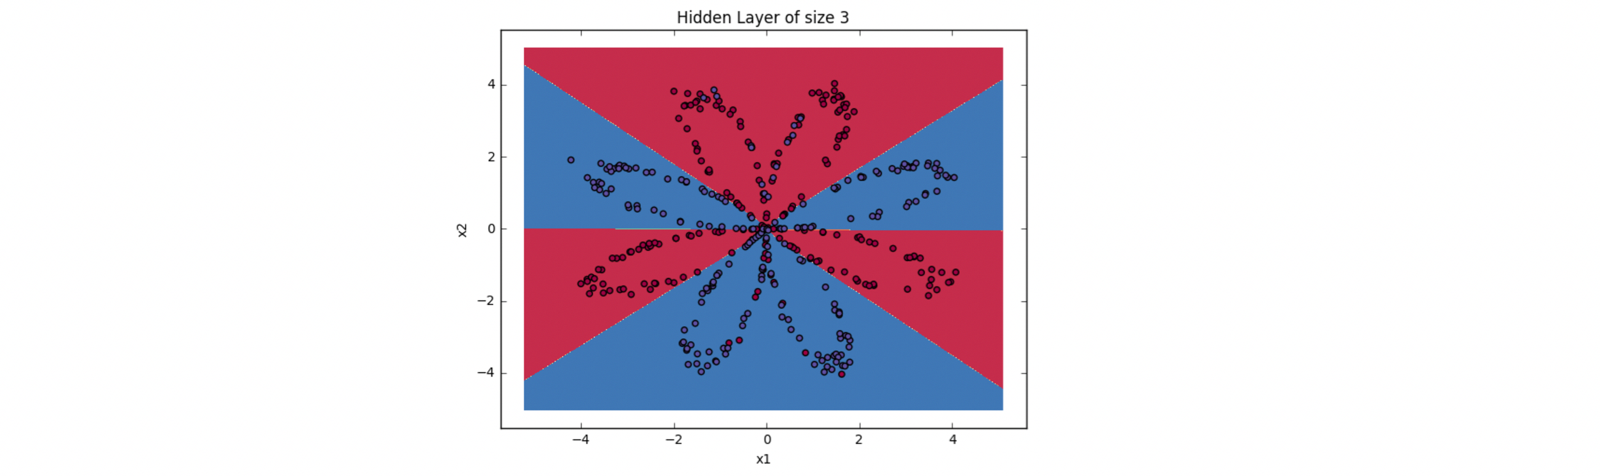
\includegraphics[width=\textwidth]{course1/Hidden_Layer}
\end{center}
\caption{classify points}
\label{fig:Hidden_Layer}
\end{figure}

By completing this assignment you will:
\begin{itemize}
\item Develop an intuition of back-propagation and see it work on data.
\item Recognize that the more hidden layers you have the more complex structure you could capture.
\item Build all the helper functions to implement a full model with one hidden layer.
\end{itemize}


You will learn how to:
\begin{itemize}
\item Implement a 2-class classification neural network with a single hidden layer
\item Use units with a non-linear activation function, such as tanh
\item Compute the cross entropy loss
\item Implement forward and backward propagation
\end{itemize}

This assignment prepares you well for the upcoming assignment. Take your time to complete it and make sure you get the expected outputs when working through the different exercises. In some code blocks, you will find a "\#GRADED FUNCTION: functionName" comment. Please do not modify it. After you are done, submit your work and check your results. You need to score 70\% to pass. Good luck :) !


\subsubsection{Packages}

Let's first import all the packages that you will need during this assignment.
\begin{itemize}
\item \href{http://www.numpy.org/}{numpy} is the fundamental package for scientific computing with Python.
\item \href{http://scikit-learn.org/stable/}{sklearn} provides simple and efficient tools for data mining and data analysis.
\item \href{https://matplotlib.org/}{matplotlib} is a library for plotting graphs in Python.
\item testCases provides some test examples to assess the correctness of your functions
\item planar\_utils provide various useful functions used in this assignment
\end{itemize}

\begin{minted}{python}
# Package imports
import numpy as np
import matplotlib.pyplot as plt
from testCases_v2 import *
import sklearn
import sklearn.datasets
import sklearn.linear_model
from planar_utils import plot_decision_boundary, sigmoid, load_planar_dataset, load_extra_datasets

#matplotlib inline

np.random.seed(1) # set a seed so that the results are consistent
\end{minted}

\subsubsection{Dataset}

First, let's get the dataset you will work on. The following code will load a "flower" 2-class dataset into variables X and Y.
\begin{minted}{python}
X, Y = load_planar_dataset()
\end{minted}

Visualize the dataset using matplotlib. The data looks like a "flower" with some red (label y=0) and some blue (y=1) points. Your goal is to build a model to fit this data.
\begin{minted}{python}
# Visualize the data:
plt.scatter(X[0, :], X[1, :], c=Y, s=40, cmap=plt.cm.Spectral);
\end{minted}

\begin{figure}[h]
\begin{center}
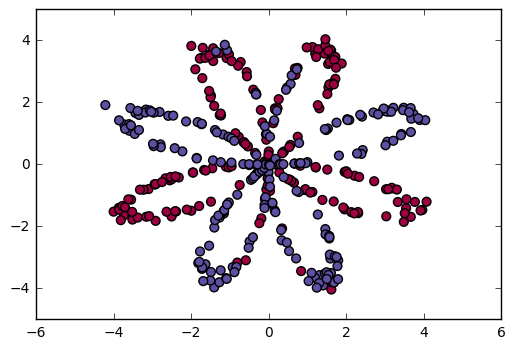
\includegraphics[width=0.6\textwidth]{course1/visualize_data}
\end{center}
\caption{Visualize the dataset}
\label{fig:visualize_data}
\end{figure}


You have:
\begin{itemize}
\item a numpy-array (matrix) X that contains your features (x1, x2)
\item a numpy-array (vector) Y that contains your labels (red:0, blue:1).
\end{itemize}

Lets first get a better sense of what our data is like.

{\textbf{Exercise}}: How many training examples do you have? In addition, what is the shape of the variables X and Y?

\begin{minted}{python}
### START CODE HERE ### (≈ 3 lines of code)
shape_X = X.shape
shape_Y = Y.shape
m = shape_X[1]  # training et size
### END CODE HERE ###

print ('The shape of X is: ' + str(shape_X))
print ('The shape of Y is: ' + str(shape_Y))
print ('I have m = %d training examples.' % (m))

#output
The shape of X is: (2, 400)
The shape of Y is: (1, 400)
I have m = 400 training examples.
\end{minted}


\subsubsection{Simple Logistic Regression}

Before building a full neural network, lets first see how logistic regression performs on this problem. You can use sklearn's built-in functions to do that. Run the code below to train a logistic regression classifier on the dataset.
\begin{minted}{python}
# Train the logistic regression classifier
clf = sklearn.linear_model.LogisticRegressionCV();
clf.fit(X.T, Y.T);
\end{minted}

You can now plot the decision boundary of these models. Run the code below
\begin{minted}{python}
# Plot the decision boundary for logistic regression
plot_decision_boundary(lambda x: clf.predict(x), X, Y)
plt.title("Logistic Regression")

# Print accuracy
LR_predictions = clf.predict(X.T)
print ('Accuracy of logistic regression: %d ' % float((np.dot(Y,LR_predictions) + np.dot(1-Y,1-LR_predictions))/float(Y.size)*100) +
       '% ' + "(percentage of correctly labelled datapoints)")
\end{minted}


The result is as follows:
\begin{minted}{python}
Accuracy of logistic regression: 47 % (percentage of correctly labelled datapoints)
\end{minted}
\begin{figure}[h]
\begin{center}
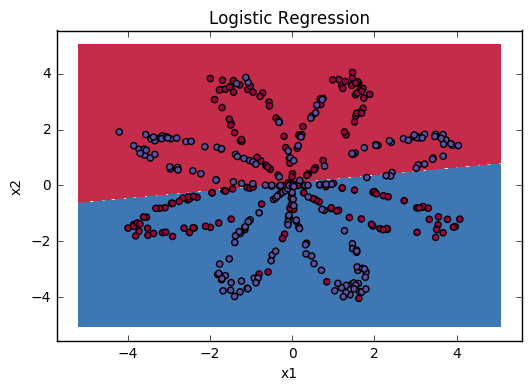
\includegraphics[width=0.6\textwidth]{course1/Logistic_Regression}
\end{center}
\caption{Logistic Regression}
\label{fig:Logistic_Regression}
\end{figure}

{\textbf {Interpretation}}: The dataset is not linearly separable, so logistic regression doesn't perform well. Hopefully a neural network will do better. Let's try this now!

\subsubsection{Neural Network model}

Logistic regression did not work well on the "flower dataset". You are going to train a Neural Network with a single hidden layer.

Here is our model:
\begin{figure}[h]
\begin{center}
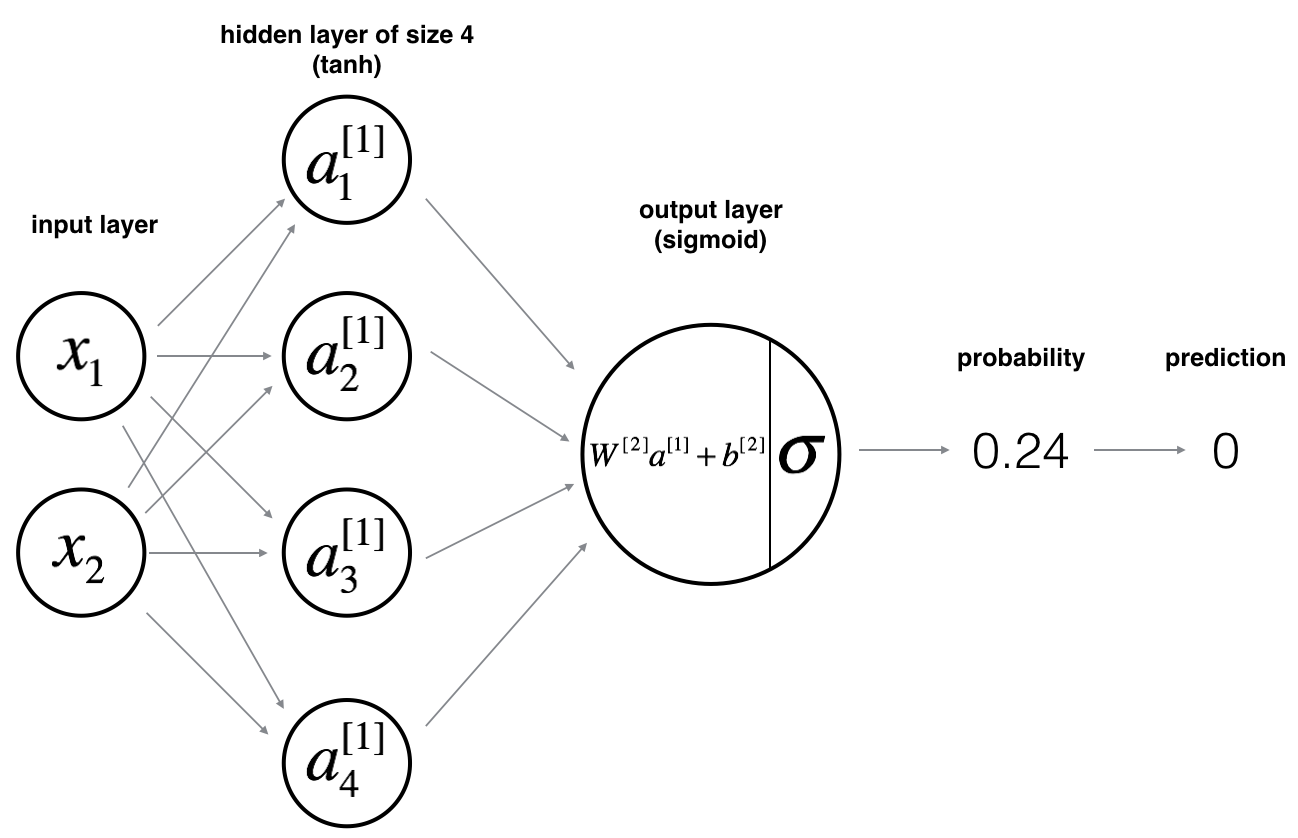
\includegraphics[width=0.6\textwidth]{course1/Neural_Network_model}
\end{center}
\caption{Neural Network Model}
\label{fig:Neural_Network_model}
\end{figure}

{\textbf {Mathematically}}:

For one example $x^{(i)}$:
\begin{align}
z^{[1] (i)} &=  W^{[1]} x^{(i)} + b^{[1] (i)}\\
a^{[1] (i)} &= \tanh(z^{[1] (i)})\\
z^{[2] (i)} &= W^{[2]} a^{[1] (i)} + b^{[2] (i)}\\
\hat{y}^{(i)} &= a^{[2] (i)} = \sigma(z^{ [2] (i)})\\
y^{(i)}_{prediction} &= \begin{cases} 1 & \mbox{if } a^{[2](i)} > 0.5 \\ 0 & \mbox{otherwise } \end{cases}
\end{align}

Given the predictions on all the examples, you can also compute the cost $J$ as follows:
\begin{align}
J = - \frac{1}{m} \sum\limits_{i = 0}^{m} \large\left(\small y^{(i)}\log\left(a^{[2] (i)}\right) + (1-y^{(i)})\log\left(1- a^{[2] (i)}\right)  \large  \right) \small 
\end{align}



{\textbf {Reminder}}: The general methodology to build a Neural Network is to:
\begin{itemize}
\item[1] Define the neural network structure ( \# of input units,  \# of hidden units, etc). 
\item[2] Initialize the model's parameters
\item[3] Loop:
\begin{itemize}
\item Implement forward propagation
\item Compute loss
\item Implement backward propagation to get the gradients
\item Update parameters (gradient descent)
\end{itemize}
\end{itemize}

You often build helper functions to compute steps 1-3 and then merge them into one function we call `nn\_model()'. Once you've built `nn\_model()' and learnt the right parameters, you can make predictions on new data.


\subsubsubsection{Defining the neural network structure}\label{section4.1}

{\textbf {Exercise}}: Define three variables:
\begin{itemize}
\item n\_x: the size of the input layer
\item n\_h: the size of the hidden layer (set this to 4) 
\item n\_y: the size of the output layer
\end{itemize}

{\textbf {Hint}}: Use shapes of X and Y to find n\_x and n\_y. Also, hard code the hidden layer size to be 4.

\begin{minted}{python}
# GRADED FUNCTION: layer_sizes

def layer_sizes(X, Y):
    """
    Arguments:
    X -- input dataset of shape (input size, number of examples)
    Y -- labels of shape (output size, number of examples)
    
    Returns:
    n_x -- the size of the input layer
    n_h -- the size of the hidden layer
    n_y -- the size of the output layer
    """
    ### START CODE HERE ### (≈ 3 lines of code)
    n_x = X.shape[0] # size of input layer
    n_h = 4
    n_y = Y.shape[0]# size of output layer
    ### END CODE HERE ###
    return (n_x, n_h, n_y)
\end{minted}



\subsubsubsection{Initialize the model's parameters}\label{section4.2}

{\textbf {Exercise}}: Implement the function initialize\_parameters().

{\textbf {Instructions}}:
\begin{itemize}
\item Make sure your parameters' sizes are right. Refer to the neural network figure above if needed.
\item You will initialize the weights matrices with random values.
\begin{itemize}
\item Use: np.random.randn(a,b) * 0.01 to randomly initialize a matrix of shape (a,b).
\end{itemize}
\item You will initialize the bias vectors as zeros.
\begin{itemize}
\item Use: np.zeros((a,b)) to initialize a matrix of shape (a,b) with zeros.
\end{itemize}
\end{itemize}

\begin{minted}{python}
# GRADED FUNCTION: initialize_parameters

def initialize_parameters(n_x, n_h, n_y):
    """
    Argument:
    n_x -- size of the input layer
    n_h -- size of the hidden layer
    n_y -- size of the output layer
    
    Returns:
    params -- python dictionary containing your parameters:
                    W1 -- weight matrix of shape (n_h, n_x)
                    b1 -- bias vector of shape (n_h, 1)
                    W2 -- weight matrix of shape (n_y, n_h)
                    b2 -- bias vector of shape (n_y, 1)
    """
    
    np.random.seed(2) # we set up a seed so that your output matches ours although the initialization is random.
    
    ### START CODE HERE ### (≈ 4 lines of code)
    W1 = np.random.randn(n_h,n_x) * 0.01
    b1 = np.zeros((n_h,1))
    W2 = np.random.randn(n_y,n_h)* 0.01
    b2 = np.zeros((n_y,1))
    ### END CODE HERE ###
    
    assert (W1.shape == (n_h, n_x))
    assert (b1.shape == (n_h, 1))
    assert (W2.shape == (n_y, n_h))
    assert (b2.shape == (n_y, 1))
    
    parameters = {"W1": W1,
                  "b1": b1,
                  "W2": W2,
                  "b2": b2}
    
    return parameters
\end{minted}



\subsubsubsection{The Loop}\label{section4.3}


{\textbf {Question}}: Implement `forward\_propagation()'.

{\textbf {Instructions}}:
\begin{itemize}
\item Look above at the mathematical representation of your classifier.
\item You can use the function `sigmoid()'. It is built-in (imported) in the notebook.
\item You can use the function `np.tanh()'. It is part of the numpy library.
\item The steps you have to implement are:
\begin{itemize}
    \item[1] Retrieve each parameter from the dictionary ``parameters" (which is the output of `initialize\_parameters()') by using `parameters[``.."]'.
    \item[2] Implement Forward Propagation. Compute $Z^{[1]}, A^{[1]}, Z^{[2]}$ and $A^{[2]}$ (the vector of all your predictions on all the examples in the training set).
\end{itemize}    
\item Values needed in the backpropagation are stored in ``cache". The \emph{cache} will be given as an input to the backpropagation function.
\end{itemize}



\begin{minted}{python}
# GRADED FUNCTION: forward_propagation

def forward_propagation(X, parameters):
    """
    Argument:
    X -- input data of size (n_x, m)
    parameters -- python dictionary containing your parameters (output of initialization function)
    
    Returns:
    A2 -- The sigmoid output of the second activation
    cache -- a dictionary containing "Z1", "A1", "Z2" and "A2"
    """
    # Retrieve each parameter from the dictionary "parameters"
    ### START CODE HERE ### (≈ 4 lines of code)
    W1 = parameters["W1"]
    b1 = parameters["b1"]
    W2 = parameters["W2"]
    b2 = parameters["b2"]
    ### END CODE HERE ###
    
    # Implement Forward Propagation to calculate A2 (probabilities)
    ### START CODE HERE ### (≈ 4 lines of code)
    Z1 = np.dot(W1,X)+b1
    A1 = np.tanh(Z1)
    Z2 = np.dot(W2,A1)+b2
    A2 = sigmoid(Z2)
    ### END CODE HERE ###
    
    assert(A2.shape == (1, X.shape[1]))
    
    cache = {"Z1": Z1,
             "A1": A1,
             "Z2": Z2,
             "A2": A2}
    
    return A2, cache
\end{minted}


Now that you have computed $A^{[2]}$ (in the Python variable ``A2"), which contains $a^{[2](i)}$ for every example, you can compute the cost function as follows:
\begin{equation}
J = - \frac{1}{m} \sum\limits_{i = 0}^{m} \large{(} \small y^{(i)}\log\left(a^{[2] (i)}\right) + (1-y^{(i)})\log\left(1- a^{[2] (i)}\right) \large{)} \small
\end{equation}

{\textbf {Exercise}}: Implement ``compute\_cost()'' to compute the value of the cost $J$.

{\textbf {Instructions}}:

There are many ways to implement the cross-entropy loss. To help you, we give you how we would have implemented
$- \sum\limits_{i=0}^{m}  y^{(i)}\log(a^{[2](i)})$:

\begin{minted}{python}
logprobs = np.multiply(np.log(A2),Y)
cost = - np.sum(logprobs)                # no need to use a for loop!
\end{minted}

(you can use either ``np.multiply()'' and then ``np.sum()'' or directly `np.dot()').

\begin{minted}{python}
# GRADED FUNCTION: compute_cost
def compute_cost(A2, Y, parameters):
    """
    Computes the cross-entropy cost given in equation (13)
    
    Arguments:
    A2 -- The sigmoid output of the second activation, of shape (1, number of examples)
    Y -- "true" labels vector of shape (1, number of examples)
    parameters -- python dictionary containing your parameters W1, b1, W2 and b2
    
    Returns:
    cost -- cross-entropy cost given equation (13)
    """
    
    m = Y.shape[1] # number of example

    # Compute the cross-entropy cost
    ### START CODE HERE ### (≈ 2 lines of code)
    logprobs = np.multiply(np.log(A2),Y)+np.multiply(np.log(1-A2),1-Y)
    cost = - np.sum(logprobs)/m
    ### END CODE HERE ###
#    use directly np.dot())
#    cost=-(np.dot(Y,np.log(A2.T))+np.dot(np.log(1-A2),(1-Y).T))/m
    
    cost = np.squeeze(cost)     # makes sure cost is the dimension we expect. 
                                # E.g., turns [[17]] into 17 
    
    return cost
\end{minted}


Using the cache computed during forward propagation, you can now implement {\textbf {backward propagatio}}.

{\textbf {Question}}: Implement the function backward\_propagation().

{\textbf {Instructions}}: Backpropagation is usually the hardest (most mathematical) part in deep learning. To help you, here again is the slide from the lecture on backpropagation. You'll want to use the six equations on the right of this slide, since you are building a vectorized implementation.

\begin{align}
\frac{\partial \mathcal{J} }{ \partial z_{2}^{(i)} } &= \frac{1}{m} (a^{[2](i)} - y^{(i)})\\
\frac{\partial \mathcal{J} }{ \partial W_2 } &= \frac{\partial \mathcal{J} }{ \partial z_{2}^{(i)} } a^{[1] (i) T} \\
\frac{\partial \mathcal{J} }{ \partial b_2 } &= \sum_i{\frac{\partial \mathcal{J} }{ \partial z_{2}^{(i)}}}
\end{align}
\begin{align}
\frac{\partial \mathcal{J} }{ \partial z_{1}^{(i)} } &=  W_2^T \frac{\partial \mathcal{J} }{ \partial z_{2}^{(i)} } * ( 1 - a^{[1] (i) 2}) \\
\frac{\partial \mathcal{J} }{ \partial W_1 } &= \frac{\partial \mathcal{J} }{ \partial z_{1}^{(i)} }  X^T \\
\frac{\partial \mathcal{J} _i }{ \partial b_1 } &= \sum_i{\frac{\partial \mathcal{J} }{ \partial z_{1}^{(i)}}}
\end{align}

\begin{itemize}
\item Note that $*$ denotes elementwise multiplication.
\item The notation you will use is common in deep learning coding:
\begin{itemize}
\item dW1 = $\frac{\partial \mathcal{J} }{ \partial W_1 }$
\item db1 = $\frac{\partial \mathcal{J} }{ \partial b_1 }$   
\item dW2 = $\frac{\partial \mathcal{J} }{ \partial W_2 }$   
\item db2 = $\frac{\partial \mathcal{J} }{ \partial b_2 }$
\end{itemize}    
\end{itemize} 
   

\begin{figure}[h]
\begin{center}
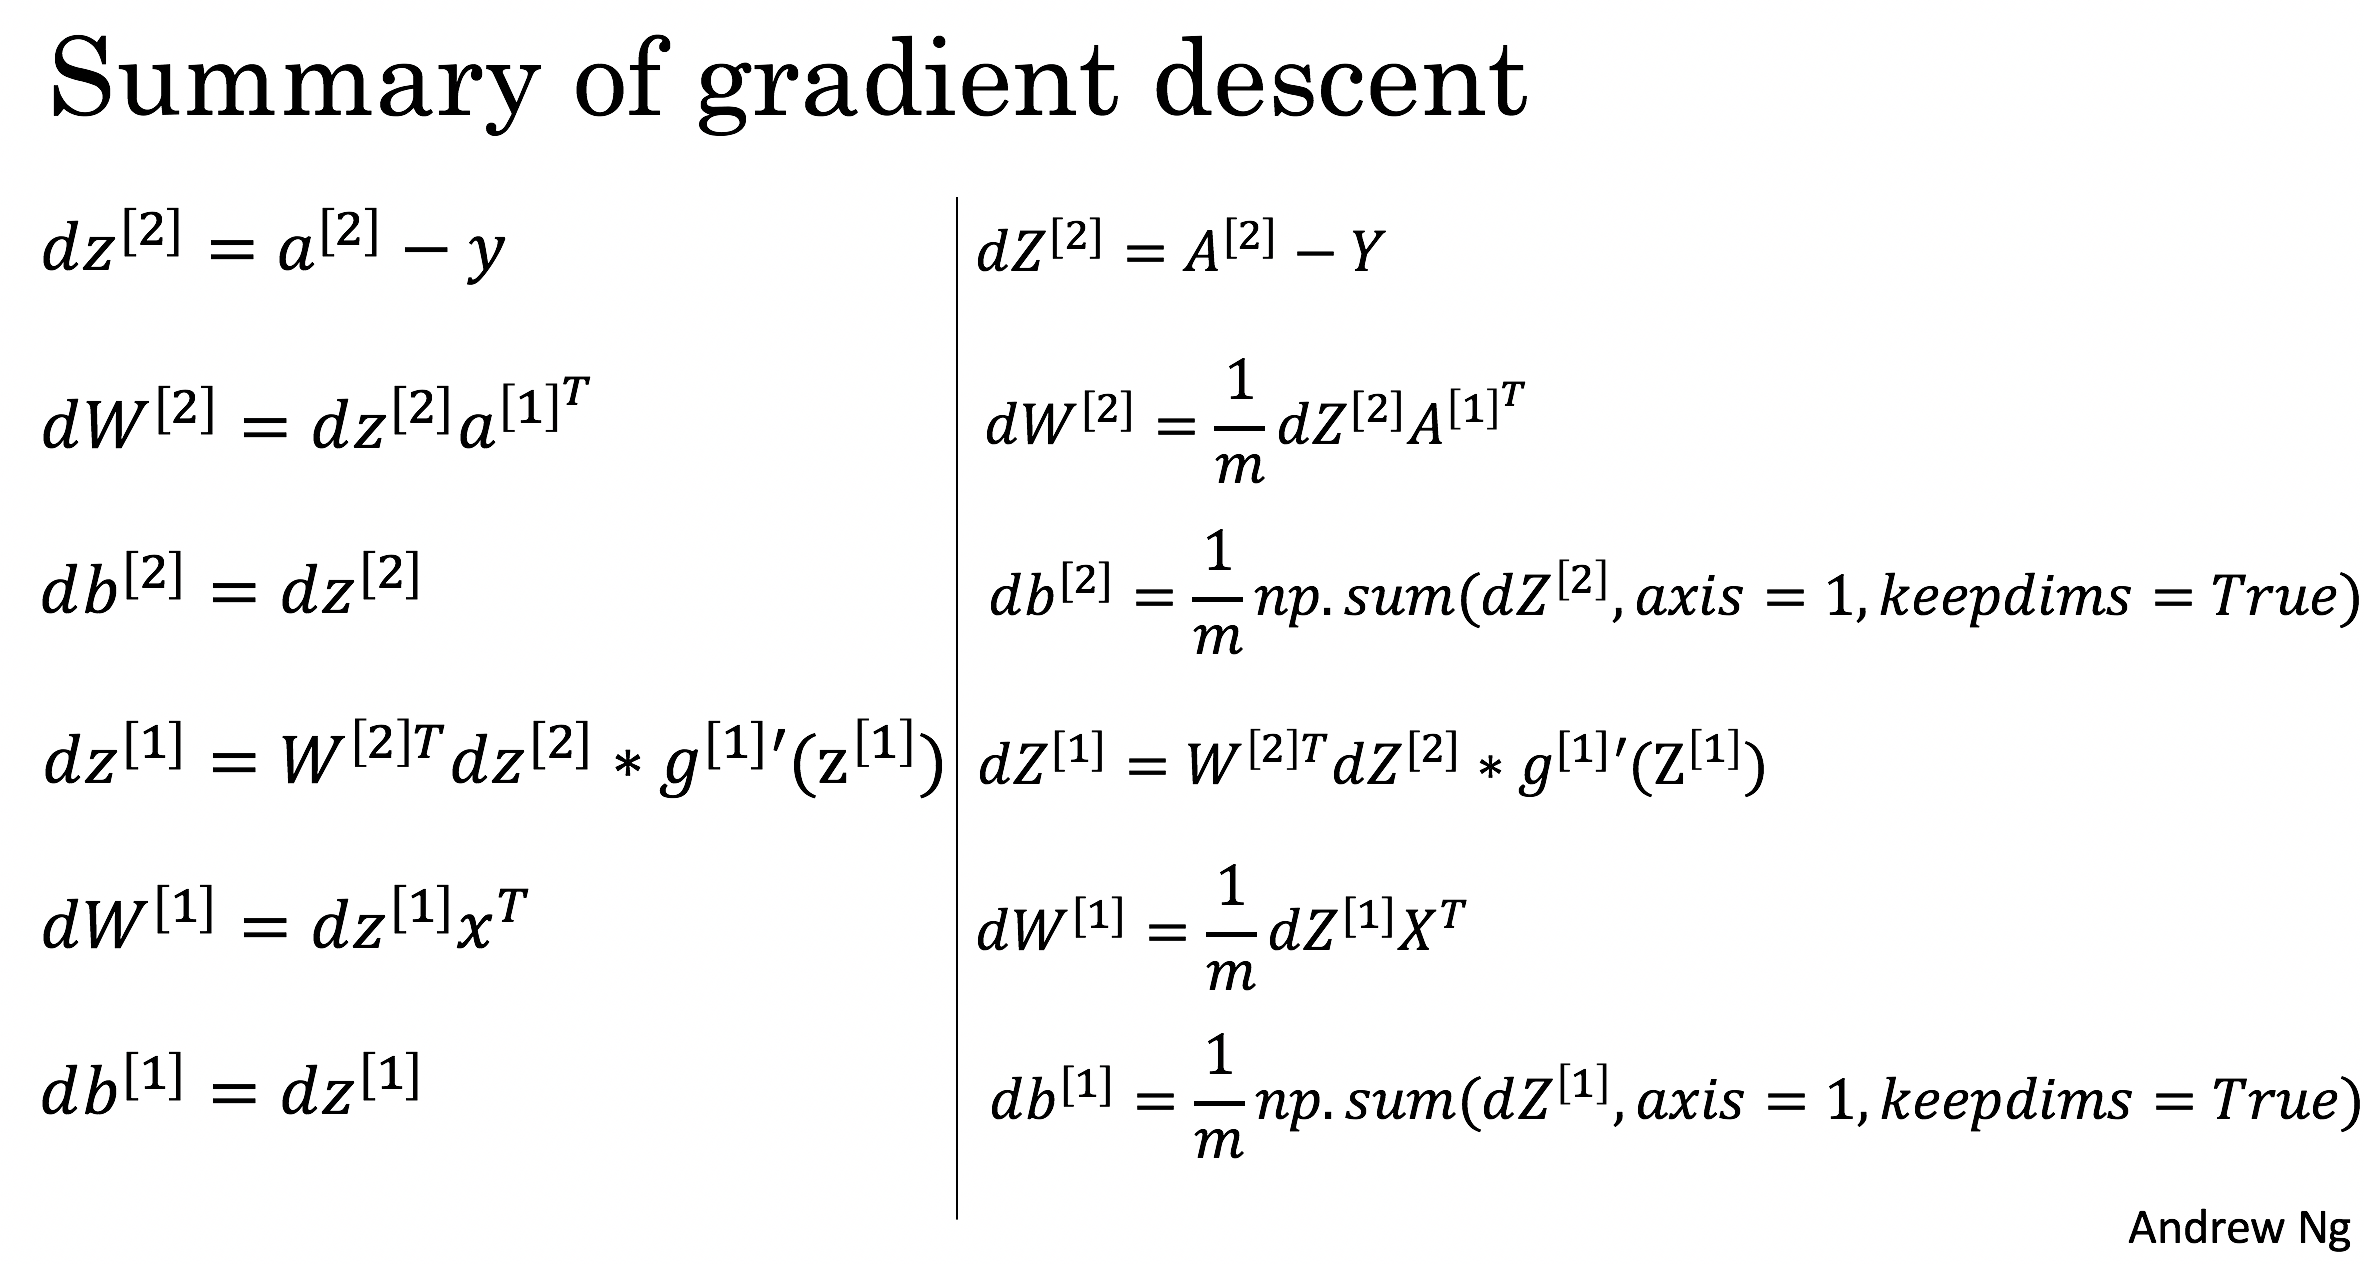
\includegraphics[width=0.9\textwidth]{course1/Backpropagation}
\end{center}
\caption{Back propagation}
\label{fig:Backpropagation}
\end{figure}

{\textbf {Tips}}:

    To compute dZ1 you'll need to compute $g^{[1]'}(Z^{[1]})$. Since $g^{[1]}(.)$ is the tanh activation function, if $a = g^{[1]}(z)$ then $g^{[1]'}(z) = 1-a^2$. So you can compute $g^{[1]'}(Z^{[1]})$ using `(1 - np.power(A1, 2))'.

\begin{minted}{python}
# GRADED FUNCTION: backward_propagation
def backward_propagation(parameters, cache, X, Y):
    """
    Implement the backward propagation using the instructions above.
    
    Arguments:
    parameters -- python dictionary containing our parameters 
    cache -- a dictionary containing "Z1", "A1", "Z2" and "A2".
    X -- input data of shape (2, number of examples)
    Y -- "true" labels vector of shape (1, number of examples)
    
    Returns:
    grads -- python dictionary containing your gradients with respect to different parameters
    """
    m = X.shape[1]
    
    # First, retrieve W1 and W2 from the dictionary "parameters".
    ### START CODE HERE ### (≈ 2 lines of code)
    W1 = parameters["W1"]
    W2 = parameters["W2"]
    ### END CODE HERE ###
        
    # Retrieve also A1 and A2 from dictionary "cache".
    ### START CODE HERE ### (≈ 2 lines of code)
    A1 = cache["A1"]
    A2 = cache["A2"]
    ### END CODE HERE ###
    
    # Backward propagation: calculate dW1, db1, dW2, db2. 
    ### START CODE HERE ### (≈ 6 lines of code, corresponding to 6 equations on slide above)
    dZ2 = A2-Y
    dW2 = np.dot(dZ2,A1.T)/m
    db2 = np.sum(dZ2,axis=1,keepdims=True)/m
    dZ1 = np.dot(W2.T,dZ2)*(1 - np.power(A1, 2))
    dW1 = np.dot(dZ1,X.T)/m
    db1 = np.sum(dZ1,axis=1,keepdims=True)/m
    ### END CODE HERE ###
    
    grads = {"dW1": dW1,
             "db1": db1,
             "dW2": dW2,
             "db2": db2}
    
    return grads
\end{minted}


{\textbf {Question}}: Implement the update rule. Use gradient descent. You have to use (dW1, db1, dW2, db2) in order to update (W1, b1, W2, b2).

{\textbf {General gradient descent rule}}: $ \theta = \theta - \alpha \frac{\partial J }{ \partial \theta }$ where $\alpha$ is the learning rate and $\theta$ represents a parameter.



\begin{minted}{python}
# GRADED FUNCTION: update_parameters
def update_parameters(parameters, grads, learning_rate = 1.2):
    """
    Updates parameters using the gradient descent update rule given above
    
    Arguments:
    parameters -- python dictionary containing your parameters 
    grads -- python dictionary containing your gradients 
    
    Returns:
    parameters -- python dictionary containing your updated parameters 
    """
    # Retrieve each parameter from the dictionary "parameters"
    ### START CODE HERE ### (≈ 4 lines of code)
    W1 = parameters["W1"]
    b1 = parameters["b1"]
    W2 = parameters["W2"]
    b2 = parameters["b2"]
    ### END CODE HERE ###

    # Retrieve each gradient from the dictionary "grads"
    ### START CODE HERE ### (≈ 4 lines of code)
    dW1 = grads["dW1"]
    db1 = grads["db1"]
    dW2 = grads["dW2"]
    db2 = grads["db2"]
    ## END CODE HERE ###
    
    # Update rule for each parameter
    ### START CODE HERE ### (≈ 4 lines of code)
    W1 = W1-learning_rate*dW1
    b1 = b1-learning_rate*db1
    W2 = W2-learning_rate*dW2
    b2 = b2-learning_rate*db2
    ### END CODE HERE ###
    
    parameters = {"W1": W1,
                  "b1": b1,
                  "W2": W2,
                  "b2": b2}
    
    return parameters
\end{minted}



\subsubsubsection{Integrate parts \ref{section4.1}, \ref{section4.2} and \ref{section4.3} in nn\_model()}

{\textbf {Question}}: Build your neural network model in nn\_model().

{\textbf {Instructions}}: The neural network model has to use the previous functions in the right order.


\begin{minted}{python}
# GRADED FUNCTION: nn_model
def nn_model(X, Y, n_h, num_iterations = 10000, print_cost=False):
    """
    Arguments:
    X -- dataset of shape (2, number of examples)
    Y -- labels of shape (1, number of examples)
    n_h -- size of the hidden layer
    num_iterations -- Number of iterations in gradient descent loop
    print_cost -- if True, print the cost every 1000 iterations
    
    Returns:
    parameters -- parameters learnt by the model. They can then be used to predict.
    """
    
    np.random.seed(3)
    n_x = layer_sizes(X, Y)[0]
    n_y = layer_sizes(X, Y)[2]
    
    # Initialize parameters, then retrieve W1, b1, W2, b2. Inputs: "n_x, n_h, n_y". Outputs = "W1, b1, W2, b2, parameters".
    ### START CODE HERE ### (≈ 5 lines of code)
    parameters = initialize_parameters(n_x, n_h, n_y)
    W1 = parameters["W1"]
    b1 = parameters["b1"]
    W2 = parameters["W2"]
    b2 = parameters["b2"]
    ### END CODE HERE ###
    
    # Loop (gradient descent)

    for i in range(0, num_iterations):
         
        ### START CODE HERE ### (≈ 4 lines of code)
        # Forward propagation. Inputs: "X, parameters". Outputs: "A2, cache".
        A2, cache =  forward_propagation(X, parameters)
        
        # Cost function. Inputs: "A2, Y, parameters". Outputs: "cost".
        cost = compute_cost(A2, Y, parameters)
 
        # Backpropagation. Inputs: "parameters, cache, X, Y". Outputs: "grads".
        grads = backward_propagation(parameters, cache, X, Y)
 
        # Gradient descent parameter update. Inputs: "parameters, grads". Outputs: "parameters".
        parameters = update_parameters(parameters, grads)
        
        ### END CODE HERE ###
        
        # Print the cost every 1000 iterations
        if print_cost and i % 1000 == 0:
            print ("Cost after iteration %i: %f" %(i, cost))

    return parameters
\end{minted}



{\textbf {Question}}: Use your model to predict by building predict().Use forward propagation to predict results.

{\textbf {Reminder}}: predictions = $y_{prediction} = \mathbb 1 \text{\{activation > 0.5\}} = \begin{cases}
      1 & \text{if}\ activation > 0.5 \\
      0 & \text{otherwise}
    \end{cases}$  
    
As an example, if you would like to set the entries of a matrix X to 0 and 1 based on a threshold you would do:\emph{ $X_{new} = (X > threshold)$}.


\begin{minted}{python}
# GRADED FUNCTION: predict
def predict(parameters, X):
    """
    Using the learned parameters, predicts a class for each example in X
    
    Arguments:
    parameters -- python dictionary containing your parameters 
    X -- input data of size (n_x, m)
    
    Returns
    predictions -- vector of predictions of our model (red: 0 / blue: 1)
    """
    
    # Computes probabilities using forward propagation, and classifies to 0/1 using 0.5 as the threshold.
    ### START CODE HERE ### (≈ 2 lines of code)
    A2, cache = forward_propagation(X, parameters)
    predictions = np.round(A2)
    ### END CODE HERE ###
    
    return predictions
\end{minted}


It is time to run the model and see how it performs on a planar dataset. Run the following code to test your model with a single hidden layer of  $n_h$  hidden units.

\begin{minted}{python}
# Build a model with a n_h-dimensional hidden layer
parameters = nn_model(X, Y, n_h = 4, num_iterations = 10000, print_cost=True)

# Plot the decision boundary
plot_decision_boundary(lambda x: predict(parameters, x.T), X, Y)
plt.title("Decision Boundary for hidden layer size " + str(4))
\end{minted}

The classification result of planar dataset is as follows:

\begin{figure}[h]
\begin{center}
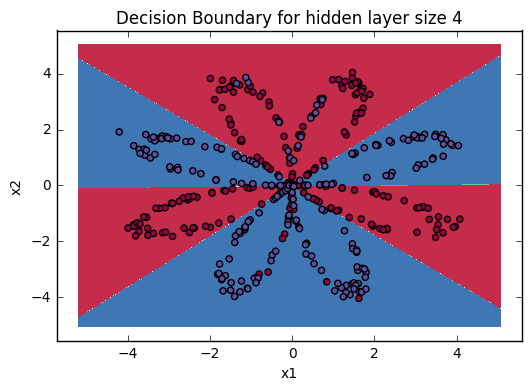
\includegraphics[width=0.6\textwidth]{course1/Decision_Boundary}
\end{center}
\caption{Decision Boundary for hidden layer size}
\label{fig:Decision_Boundary}
\end{figure}

\begin{minted}{python}
# Print accuracy
predictions = predict(parameters, X)
print ('Accuracy: %d' % float((np.dot(Y,predictions.T) + np.dot(1-Y,1-predictions.T))/float(Y.size)*100) + '%')

#Accuracy
Accuracy: 90%
\end{minted}


Accuracy is really high compared to Logistic Regression. The model has learnt the leaf patterns of the flower! Neural networks are able to learn even highly non-linear decision boundaries, unlike logistic regression.

Now, let's try out several hidden layer sizes.


\subsubsubsection{Tuning hidden layer size (optional/ungraded exercise)}

Run the following code. It may take 1-2 minutes. You will observe different behaviors of the model for various hidden layer sizes.

\begin{minted}{python}
# This may take about 2 minutes to run

plt.figure(figsize=(16, 32))
hidden_layer_sizes = [1, 2, 3, 4, 5, 20, 50]
for i, n_h in enumerate(hidden_layer_sizes):
    plt.subplot(5, 2, i+1)
    plt.title('Hidden Layer of size %d' % n_h)
    parameters = nn_model(X, Y, n_h, num_iterations = 5000)
    plot_decision_boundary(lambda x: predict(parameters, x.T), X, Y)
    predictions = predict(parameters, X)
    accuracy = float((np.dot(Y,predictions.T) + np.dot(1-Y,1-predictions.T))/float(Y.size)*100)
    print ("Accuracy for {} hidden units: {} %".format(n_h, accuracy))
\end{minted}

\begin{figure}
\begin{center}
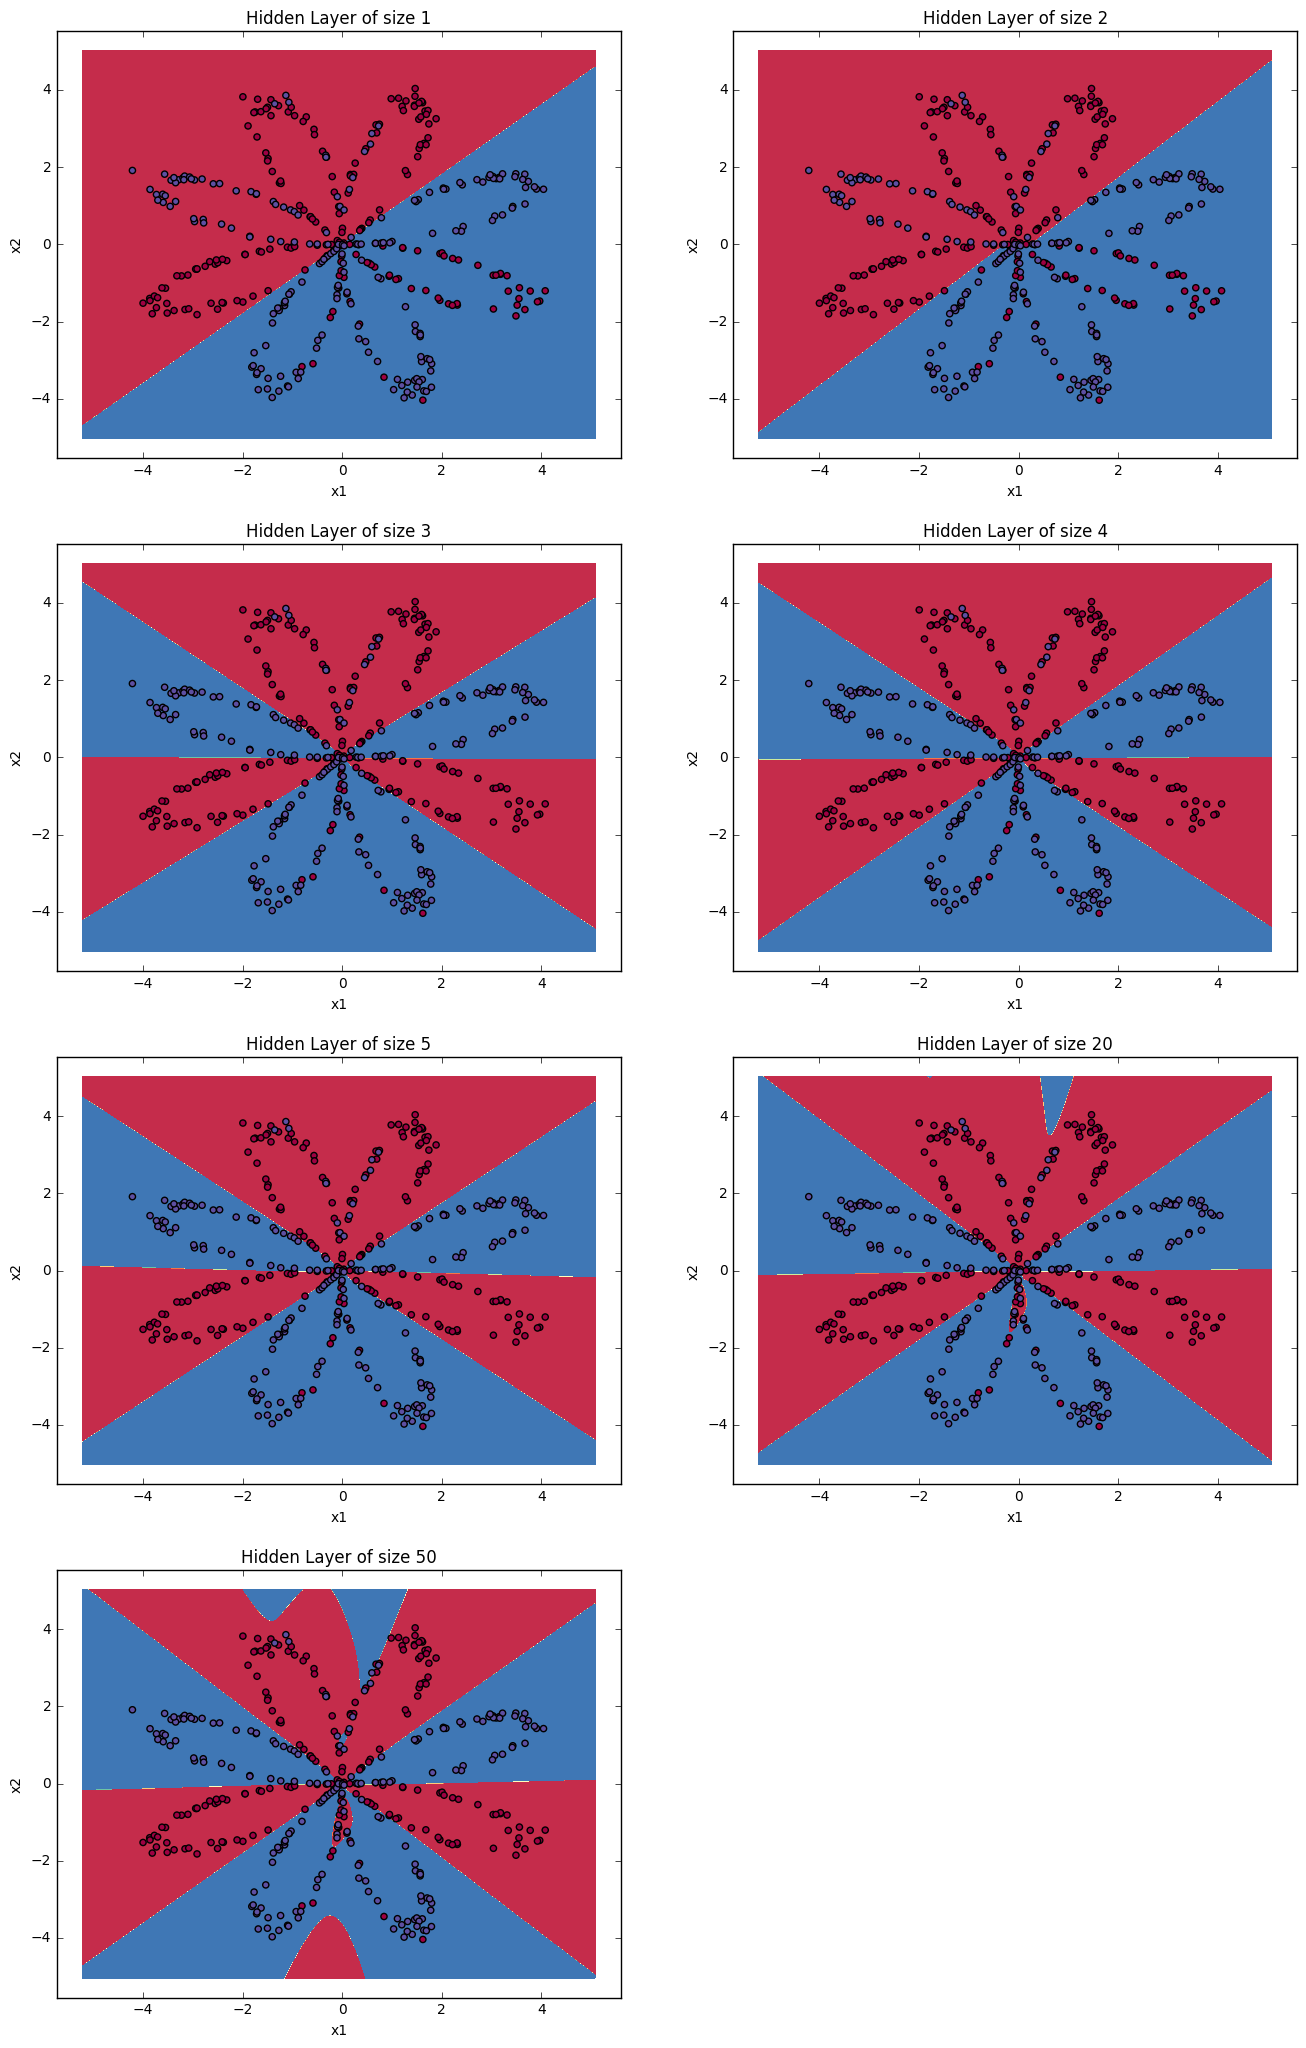
\includegraphics[width=\textwidth]{course1/various_hidden_layer_sizes}
\end{center}
\vspace{-0.5cm}
\caption{Different behaviors of the model for various hidden layer sizes}
\label{fig:various_hidden_layer_sizes}
\end{figure}


{\textbf {Interpretation}}:
\begin{itemize}
\item The larger models (with more hidden units) are able to fit the training set better, until eventually the largest models overfit the data.
\item The best hidden layer size seems to be around $n_h = 5$. Indeed, a value around here seems to fits the data well without also incurring noticable overfitting.
\item You will also learn later about regularization, which lets you use very large models (such as $n_h = 50$) without much overfitting.
\end{itemize}

{\color{blue}\textbf {
You've learnt to:
\begin{itemize}
\item Build a complete neural network with a hidden layer
\item Make a good use of a non-linear unit
\item Implemented forward propagation and backpropagation, and trained a neural network
\item See the impact of varying the hidden layer size, including overfitting.
\end{itemize}
}}

\clearpage
\subsubsection{Code of Neural Network With a Hidden Layer}
\begin{minted}{python}
# Package imports
import numpy as np
import matplotlib.pyplot as plt
from testCases_v2 import *
import sklearn
import sklearn.datasets
import sklearn.linear_model
from planar_utils import plot_decision_boundary, sigmoid, load_planar_dataset, load_extra_datasets

#matplotlib inline

np.random.seed(1) # set a seed so that the results are consistent

X, Y = load_planar_dataset()

# Visualize the data:
#plt.scatter(X[0, :], X[1, :], c=Y, s=40, cmap=plt.cm.Spectral);

shape_X = X.shape
shape_Y = Y.shape
m = shape_X[1]  # training set size

# Train the logistic regression classifier
#===================================
# clf = sklearn.linear_model.LogisticRegressionCV();
# clf.fit(X.T, Y.T);
# 
# # Plot the decision boundary for logistic regression
# plot_decision_boundary(lambda x: clf.predict(x), X, Y)
# plt.title("Logistic Regression")
# # Print accuracy
# LR_predictions = clf.predict(X.T)
# print ('Accuracy of logistic regression: %d ' %float((np.dot(Y,LR_predictions) +np.dot(1-Y,1-LR_predictions))/float(Y.size)*100) +'% ' + "(percentage of correctly labelled datapoints)")      
#===================================

# GRADED FUNCTION: layer_sizes
def layer_sizes(X, Y):
    """
    Arguments:
    X -- input dataset of shape (input size, number of examples)
    Y -- labels of shape (output size, number of examples)
    
    Returns:
    n_x -- the size of the input layer
    n_h -- the size of the hidden layer
    n_y -- the size of the output layer
    """
    n_x = X.shape[0] # size of input layer
    n_h = 4
    n_y = Y.shape[0]# size of output layer
    return (n_x, n_h, n_y)       
       

# GRADED FUNCTION: initialize_parameters
def initialize_parameters(n_x, n_h, n_y):
    """
    Argument:
    n_x -- size of the input layer
    n_h -- size of the hidden layer
    n_y -- size of the output layer
    
    Returns:
    params -- python dictionary containing your parameters:
                    W1 -- weight matrix of shape (n_h, n_x)
                    b1 -- bias vector of shape (n_h, 1)
                    W2 -- weight matrix of shape (n_y, n_h)
                    b2 -- bias vector of shape (n_y, 1)
    """
    
    np.random.seed(2) # we set up a seed so that your output matches ours although the initialization is random.
    
    W1 = np.random.randn(n_h,n_x) * 0.01
    b1 = np.zeros((n_h,1))
    W2 = np.random.randn(n_y,n_h)* 0.01
    b2 = np.zeros((n_y,1))
    
    assert (W1.shape == (n_h, n_x))
    assert (b1.shape == (n_h, 1))
    assert (W2.shape == (n_y, n_h))
    assert (b2.shape == (n_y, 1))
    
    parameters = {"W1": W1,
                  "b1": b1,
                  "W2": W2,
                  "b2": b2}
    
    return parameters


# GRADED FUNCTION: forward_propagation
def forward_propagation(X, parameters):
    """
    Argument:
    X -- input data of size (n_x, m)
    parameters -- python dictionary containing your parameters (output of initialization function)
    
    Returns:
    A2 -- The sigmoid output of the second activation
    cache -- a dictionary containing "Z1", "A1", "Z2" and "A2"
    """
    # Retrieve each parameter from the dictionary "parameters"
    W1 = parameters["W1"]
    b1 = parameters["b1"]
    W2 = parameters["W2"]
    b2 = parameters["b2"]
    
    # Implement Forward Propagation to calculate A2 (probabilities)
    Z1 = np.dot(W1,X)+b1
    A1 = np.tanh(Z1)
    Z2 = np.dot(W2,A1)+b2
    A2 = sigmoid(Z2)
    
    assert(A2.shape == (1, X.shape[1]))
    
    cache = {"Z1": Z1,
             "A1": A1,
             "Z2": Z2,
             "A2": A2}
    
    return A2, cache


# GRADED FUNCTION: compute_cost
def compute_cost(A2, Y, parameters):
    """
    Computes the cross-entropy cost given in equation (13)
    
    Arguments:
    A2 -- The sigmoid output of the second activation, of shape (1, number of examples)
    Y -- "true" labels vector of shape (1, number of examples)
    parameters -- python dictionary containing your parameters W1, b1, W2 and b2
    
    Returns:
    cost -- cross-entropy cost given equation (13)
    """
    
    m = Y.shape[1] # number of example

    # Compute the cross-entropy cost
    logprobs = np.multiply(np.log(A2),Y)+np.multiply(np.log(1-A2),1-Y)
    cost = - np.sum(logprobs)/m

#    use directly np.dot())
#    cost=-(np.dot(Y,np.log(A2.T))+np.dot(np.log(1-A2),(1-Y).T))/m
    
    cost = np.squeeze(cost)     # makes sure cost is the dimension we expect. 
                                # E.g., turns [[17]] into 17 
    
    return cost


# GRADED FUNCTION: backward_propagation
def backward_propagation(parameters, cache, X, Y):
    """
    Implement the backward propagation using the instructions above.
    
    Arguments:
    parameters -- python dictionary containing our parameters 
    cache -- a dictionary containing "Z1", "A1", "Z2" and "A2".
    X -- input data of shape (2, number of examples)
    Y -- "true" labels vector of shape (1, number of examples)
    
    Returns:
    grads -- python dictionary containing your gradients with respect to different parameters
    """
    m = X.shape[1]
    
    # First, retrieve W1 and W2 from the dictionary "parameters".
    W1 = parameters["W1"]
    W2 = parameters["W2"]
        
    # Retrieve also A1 and A2 from dictionary "cache".
    A1 = cache["A1"]
    A2 = cache["A2"]
    
    # Backward propagation: calculate dW1, db1, dW2, db2. 
    dZ2 = A2-Y
    dW2 = np.dot(dZ2,A1.T)/m
    db2 = np.sum(dZ2,axis=1,keepdims=True)/m
    dZ1 = np.dot(W2.T,dZ2)*(1 - np.power(A1, 2))
    dW1 = np.dot(dZ1,X.T)/m
    db1 = np.sum(dZ1,axis=1,keepdims=True)/m
    
    grads = {"dW1": dW1,
             "db1": db1,
             "dW2": dW2,
             "db2": db2}
    
    return grads


# GRADED FUNCTION: update_parameters
def update_parameters(parameters, grads, learning_rate = 1.2):
    """
    Updates parameters using the gradient descent update rule given above
    
    Arguments:
    parameters -- python dictionary containing your parameters 
    grads -- python dictionary containing your gradients 
    
    Returns:
    parameters -- python dictionary containing your updated parameters 
    """
    # Retrieve each parameter from the dictionary "parameters"
    W1 = parameters["W1"]
    b1 = parameters["b1"]
    W2 = parameters["W2"]
    b2 = parameters["b2"]

    # Retrieve each gradient from the dictionary "grads"
    dW1 = grads["dW1"]
    db1 = grads["db1"]
    dW2 = grads["dW2"]
    db2 = grads["db2"]
    
    # Update rule for each parameter
    W1 = W1-learning_rate*dW1
    b1 = b1-learning_rate*db1
    W2 = W2-learning_rate*dW2
    b2 = b2-learning_rate*db2
    
    parameters = {"W1": W1,
                  "b1": b1,
                  "W2": W2,
                  "b2": b2}
    
    return parameters



# GRADED FUNCTION: nn_model
def nn_model(X, Y, n_h, num_iterations = 10000, print_cost=False):
    """
    Arguments:
    X -- dataset of shape (2, number of examples)
    Y -- labels of shape (1, number of examples)
    n_h -- size of the hidden layer
    num_iterations -- Number of iterations in gradient descent loop
    print_cost -- if True, print the cost every 1000 iterations
    
    Returns:
    parameters -- parameters learnt by the model. They can then be used to predict.
    """
    
    np.random.seed(3)
    n_x = layer_sizes(X, Y)[0]
    n_y = layer_sizes(X, Y)[2]
    
    # Initialize parameters, then retrieve W1, b1, W2, b2. Inputs: "n_x, n_h, n_y". Outputs = "W1, b1, W2, b2, parameters".
    parameters = initialize_parameters(n_x, n_h, n_y)
    W1 = parameters["W1"]
    b1 = parameters["b1"]
    W2 = parameters["W2"]
    b2 = parameters["b2"]
    
    # Loop (gradient descent)

    for i in range(0, num_iterations):
         
        # Forward propagation. Inputs: "X, parameters". Outputs: "A2, cache".
        A2, cache =  forward_propagation(X, parameters)
        
        # Cost function. Inputs: "A2, Y, parameters". Outputs: "cost".
        cost = compute_cost(A2, Y, parameters)
 
        # Backpropagation. Inputs: "parameters, cache, X, Y". Outputs: "grads".
        grads = backward_propagation(parameters, cache, X, Y)
 
        # Gradient descent parameter update. Inputs: "parameters, grads". Outputs: "parameters".
        parameters = update_parameters(parameters, grads)
        
        
        # Print the cost every 1000 iterations
        if print_cost and i % 1000 == 0:
            print ("Cost after iteration %i: %f" %(i, cost))

    return parameters


#GRADED FUNCTION: predict
def predict(parameters, X):
    """
    Using the learned parameters, predicts a class for each example in X
    
    Arguments:
    parameters -- python dictionary containing your parameters 
    X -- input data of size (n_x, m)
    
    Returns
    predictions -- vector of predictions of our model (red: 0 / blue: 1)
    """
    
    # Computes probabilities using forward propagation, and classifies to 0/1 using 0.5 as the threshold.
    A2, cache = forward_propagation(X, parameters)
    predictions = np.round(A2)
    
    return predictions


# Build a model with a n_h-dimensional hidden layer
parameters = nn_model(X, Y, n_h = 4, num_iterations = 10000, print_cost=True)
plot_decision_boundary(lambda x: predict(parameters, x.T), X, Y)
plt.title("Decision Boundary for hidden layer size " + str(4))
print ('Accuracy: %d' % float((np.dot(Y,predictions.T) + np.dot(1-Y,1-predictions.T))/float(Y.size)*100) + '%')
\end{minted}


\clearpage
\subsection{Building your Deep Neural Network: Step by Step}

Welcome to your third programming exercise of the deep learning specialization. You will implement all the building blocks of a neural network and use these building blocks in the next assignment to build a neural network of any architecture you want. By completing this assignment you will:
\begin{itemize}
\item Develop an intuition of the over all structure of a neural network.

\item Write functions (e.g. forward propagation, backward propagation, logistic loss, etc...) that would help you decompose your code and ease the process of building a neural network.

\item Initialize/update parameters according to your desired structure.
\end{itemize}

This assignment prepares you well for the upcoming assignment. In the next assignment, you will use these functions to build a deep neural network for image classification. Take your time to complete it and make sure you get the expected outputs when working through the different exercises. In some code blocks, you will find a "\#GRADED FUNCTION: functionName" comment. Please do not modify it. After you are done, submit your work and check your results. You need to score 70\% to pass. Good luck :) !


After this assignment you will be able to:
\begin{itemize}
\item Use non-linear units like ReLU to improve your model
\item Build a deeper neural network (with more than 1 hidden layer)
\item Implement an easy-to-use neural network class
\end{itemize}


{\textbf {Notation}}:
\begin{itemize}
\item Superscript $[l]$ denotes a quantity associated with the $l^{th}$ layer. 
\begin{itemize}
\item Example: $a^{[L]}$ is the $L^{th}$ layer activation. $W^{[L]}$ and $b^{[L]}$ are the $L^{th}$ layer parameters.
\end{itemize}
\item Superscript $(i)$ denotes a quantity associated with the $i^{th}$ example. 
\begin{itemize}
\item Example: $x^{(i)}$ is the $i^{th}$ training example.
\end{itemize}
\item Lowerscript $i$ denotes the $i^{th}$ entry of a vector.
\begin{itemize}
\item Example: $a^{[l]}_i$ denotes the $i^{th}$ entry of the $l^{th}$ layer's activations).
\end{itemize}
\end{itemize}

Let's get started!


\subsubsection{Packages}

Let's first import all the packages that you will need during this assignment. 
\begin{itemize}
\item \href{www.numpy.org}{numpy} is the main package for scientific computing with Python.
\item \href{http://matplotlib.org}{matplotlib} is a library to plot graphs in Python.
\item dnn\_utils provides some necessary functions for this notebook.
\item testCases provides some test cases to assess the correctness of your functions
\item np.random.seed(1) is used to keep all the random function calls consistent. It will help us grade your work. Please don't change the seed. 
\end{itemize}

\subsubsection{Outline of the Assignment}

To build your neural network, you will be implementing several``helper functions". These helper functions will be used in the next assignment to build a two-layer neural network and an L-layer neural network. Each small helper function you will implement will have detailed instructions that will walk you through the necessary steps. Figure \ref{fig:final_outline} is an outline of this assignment, you will:

\begin{itemize}
\item Initialize the parameters for a two-layer network and for an $L$-layer neural network.
\item Implement the forward propagation module (shown in purple in the figure below).
     \begin{itemize}
     \item Complete the LINEAR part of a layer's forward propagation step (resulting in $Z^{[l]}$).
     \item We give you the ACTIVATION function (relu/sigmoid).
     \item Combine the previous two steps into a new [LINEAR->ACTIVATION] forward function.
     \item Stack the [LINEAR->RELU] forward function L-1 time (for layers 1 through L-1) and add a [LINEAR->SIGMOID] at the end (for the final layer $L$). This gives you a new L\_model\_forward function.
     \end{itemize}
\item Compute the loss.
\item Implement the backward propagation module (denoted in red in the figure below).
   \begin{itemize}
    \item Complete the LINEAR part of a layer's backward propagation step.
    \item We give you the gradient of the ACTIVATE function (relu\_backward/sigmoid\_backward) 
    \item Combine the previous two steps into a new [LINEAR->ACTIVATION] backward function.
    \item Stack [LINEAR->RELU] backward L-1 times and add [LINEAR->SIGMOID] backward in a new L\_model\_backward function
    \end{itemize}
\item Finally update the parameters.
\end{itemize}

\begin{figure}[h]
\begin{center}
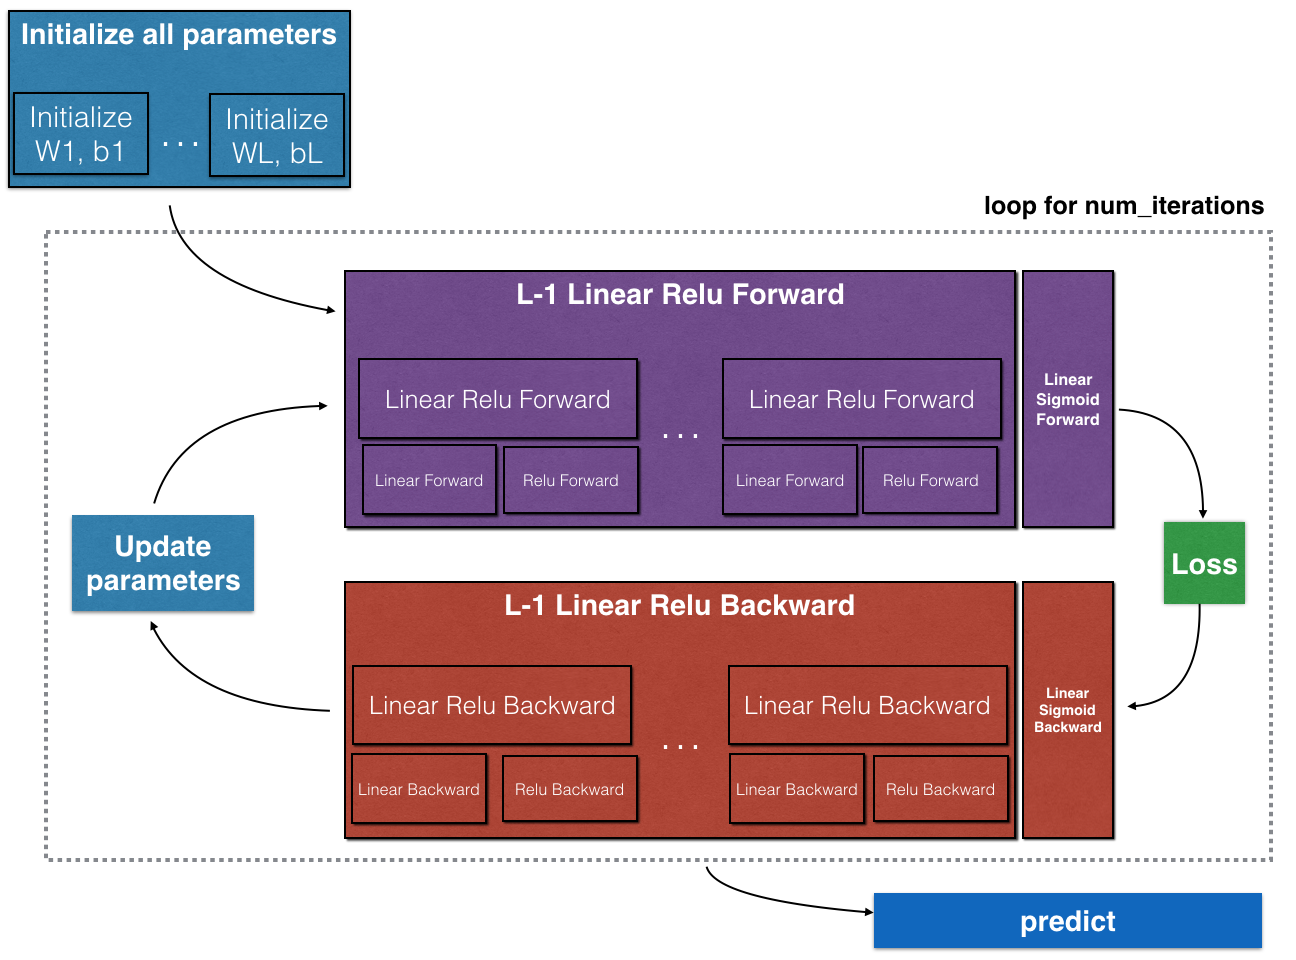
\includegraphics[width=0.5\textwidth]{course1/final_outline}
\end{center}
\caption{Outline}
\label{fig:final_outline}
\end{figure}

{\textbf {Note}} that for every forward function, there is a corresponding backward function. That is why at every step of your forward module you will be storing some values in a cache. The cached values are useful for computing gradients. In the backpropagation module you will then use the cache to calculate the gradients. This assignment will show you exactly how to carry out each of these steps.



\subsubsection{Initialization}

You will write two helper functions that will initialize the parameters for your model. The first function will be used to initialize parameters for a two layer model. The second one will generalize this initialization process to  $L$ layers.

\subsubsubsection{2-layer Neural Network}

{\textbf {Exercise}}: Create and initialize the parameters of the 2-layer neural network.

{\textbf {Instructions}}:
\begin{itemize}
\item The model's structure is: LINEAR -> RELU -> LINEAR -> SIGMOID.
\item Use random initialization for the weight matrices. Use np.random.randn(shape)*0.01 with the correct shape.
\item Use zero initialization for the biases. Use np.zeros(shape).
\end{itemize}

\begin{minted}{python}
# GRADED FUNCTION: initialize_parameters
def initialize_parameters(n_x, n_h, n_y):
    """
    Argument:
    n_x -- size of the input layer
    n_h -- size of the hidden layer
    n_y -- size of the output layer
    
    Returns:
    parameters -- python dictionary containing your parameters:
                    W1 -- weight matrix of shape (n_h, n_x)
                    b1 -- bias vector of shape (n_h, 1)
                    W2 -- weight matrix of shape (n_y, n_h)
                    b2 -- bias vector of shape (n_y, 1)
    """
    
    np.random.seed(1)
    
    ### START CODE HERE ### (≈ 4 lines of code)
    W1 = np.random.randn(n_h, n_x)*0.01
    b1 = np.zeros((n_h, 1))
    W2 = np.random.randn(n_y, n_h)*0.01
    b2 = np.zeros((n_y, 1))
    ### END CODE HERE ###
    
    assert(W1.shape == (n_h, n_x))
    assert(b1.shape == (n_h, 1))
    assert(W2.shape == (n_y, n_h))
    assert(b2.shape == (n_y, 1))
    
    parameters = {"W1": W1,
                  "b1": b1,
                  "W2": W2,
                  "b2": b2}
    
    return parameters
\end{minted}


\subsubsubsection{L-layer Neural Network}

The initialization for a deeper L-layer neural network is more complicated because there are many more weight matrices and bias vectors. When completing the ``initialize\_parameters\_deep'', you should make sure that your dimensions match between each layer. Recall that $n^{[l]}$ is the number of units in layer $l$. Thus for example if the size of our input $X$ is $(12288, 209)$ (with $m=209$ examples) then:


\begin{table}[H]
\centering
\begin{tabular}{ccccc}  
\toprule
 & Shape of W & Shape of b & Activation & Shape of Activation\\
\midrule
Layer 1 & $(n^{[1]},12288)$ & $(n^{[1]},1)$  & $Z^{[1]} = W^{[1]}  X + b^{[1]} $  & $(n^{[1]},209)$ \\
Layer 2 & $(n^{[2]}, n^{[1]})$ & $(n^{[2]},1)$  & $Z^{[2]} = W^{[2]} A^{[1]} + b^{[2]}$   & $(n^{[2]}, 209)$ \\
$\vdots$  & $\vdots$  & $\vdots$   & $\vdots$   & $\vdots$  \\
Layer L-1  & $(n^{[L-1]}, n^{[L-2]})$  & $(n^{[L-1]}, 1)$   & $Z^{[L-1]} =  W^{[L-1]} A^{[L-2]} + b^{[L-1]}$ & $(n^{[L-1]}, 209)$  \\
Layer L  & $(n^{[L]}, n^{[L-1]})$ & $(n^{[L]}, 1)$  & $Z^{[L]} =  W^{[L]} A^{[L-1]} + b^{[L]}$ & $(n^{[L]}, 209)$  \\
\bottomrule
\end{tabular}
\end{table}

Remember that when we compute $W X + b$ in python, it carries out broadcasting. For example, if: 
\begin{center}
$ W = \begin{bmatrix}
    j  & k  & l\\
    m  & n & o \\
    p  & q & r 
\end{bmatrix}\;\;\; X = \begin{bmatrix}
    a  & b  & c\\
    d  & e & f \\
    g  & h & i 
\end{bmatrix} \;\;\; b =\begin{bmatrix}
    s  \\
    t  \\
    u
\end{bmatrix}$
\end{center}

Then $WX + b$ will be:
\begin{equation}
WX + b = \begin{bmatrix}
    (ja + kd + lg) + s  & (jb + ke + lh) + s  & (jc + kf + li)+ s\\
    (ma + nd + og) + t & (mb + ne + oh) + t & (mc + nf + oi) + t\\
    (pa + qd + rg) + u & (pb + qe + rh) + u & (pc + qf + ri)+ u
\end{bmatrix}
\end{equation}


{\textbf {Exercise}}: Implement initialization for an L-layer Neural Network.

{\textbf {Instructions}}:
\begin{itemize}
\item The model's structure is [LINEAR -> RELU] $ \times$ (L-1) -> LINEAR -> SIGMOID. I.e., it has $L-1$ layers using a ReLU activation function followed by an output layer with a sigmoid activation function.
\item Use random initialization for the weight matrices. Use ``np.random.rand(shape) * 0.01''.
\item Use zeros initialization for the biases. Use ``np.zeros(shape)''.
\item We will store $n^{[l]}$, the number of units in different layers, in a variable ``layer\_dims''. For example, the ``layer\_dims'' for the ``Planar Data classification mode'' from last week would have been [2,4,1]: There were two inputs, one hidden layer with 4 hidden units, and an output layer with 1 output unit. Thus means ``W1'''s shape was (4,2), ``b1'' was (4,1), ``W2'' was (1,4) and ``b2'' was (1,1). Now you will generalize this to $L$ layers! 
\item Here is the implementation for $L=1$ (one layer neural network). It should inspire you to implement the general case (L-layer neural network).
\end{itemize}

\begin{mypython}
    if L == 1:
        parameters["W" + str(L)] = np.random.randn(layer_dims[1], layer_dims[0]) * 0.01
        parameters["b" + str(L)] = np.zeros((layer_dims[1], 1))
\end{mypython}




\begin{minted}{python}
# GRADED FUNCTION: initialize_parameters_deep
def initialize_parameters_deep(layer_dims):
    """
    Arguments:
    layer_dims -- python array (list) containing the dimensions of each layer in our network
    
    Returns:
    parameters -- python dictionary containing your parameters "W1", "b1", ..., "WL", "bL":
      Wl -- weight matrix of shape (layer_dims[l], layer_dims[l-1])
      bl -- bias vector of shape (layer_dims[l], 1)
    """
    
    np.random.seed(3)
    parameters = {}
    L = len(layer_dims)            # number of layers in the network

    for l in range(1, L):
        ### START CODE HERE ### (≈ 2 lines of code)
        parameters['W' + str(l)] = np.random.randn(layer_dims[l], layer_dims[l-1]) * 0.01
        parameters['b' + str(l)] = np.zeros((layer_dims[l], 1))
        ### END CODE HERE ###
        
        assert(parameters['W' + str(l)].shape == (layer_dims[l], layer_dims[l-1]))
        assert(parameters['b' + str(l)].shape == (layer_dims[l], 1))

        
    return parameters
\end{minted}



\subsubsection{Forward propagation module}
\subsubsubsection{Linear Forward}

Now that you have initialized your parameters, you will do the forward propagation module. You will start by implementing some basic functions that you will use later when implementing the model. You will complete three functions in this order:
\begin{itemize}
\item[1] LINEAR

\item[2] LINEAR -> ACTIVATION where ACTIVATION will be either ReLU or Sigmoid

\item[3] [LINEAR -> RELU] $\times$ (L-1) -> LINEAR -> SIGMOID (whole model)
\end{itemize}

The linear forward module (vectorized over all the examples) computes the following equations:
\begin{equation}
Z^{[l]} = W^{[l]}A^{[l-1]} +b^{[l]}
\end{equation}
where $A^{[0]} = X$. 

{\textbf {Exercise}}: Build the linear part of forward propagation.

{\textbf {Reminder}:
The mathematical representation of this unit is $Z^{[l]} = W^{[l]}A^{[l-1]} +b^{[l]}$. You may also find ``np.dot()'' useful. If your dimensions don't match, printing ``W.shape'' may help.

\begin{minted}{python}
# GRADED FUNCTION: linear_forward
def linear_forward(A, W, b):
    """
    Implement the linear part of a layer's forward propagation.

    Arguments:
    A -- activations from previous layer (or input data): (size of previous layer, number of examples)
    W -- weights matrix: numpy array of shape (size of current layer, size of previous layer)
    b -- bias vector, numpy array of shape (size of the current layer, 1)

    Returns:
    Z -- the input of the activation function, also called pre-activation parameter 
    cache -- a python dictionary containing "A", "W" and "b" ; stored for computing the backward pass efficiently
    """
    
    ### START CODE HERE ### (≈ 1 line of code)
    Z = np.dot(W,A)+b
    ### END CODE HERE ###
    
    assert(Z.shape == (W.shape[0], A.shape[1]))
    cache = (A, W, b)
    
    return Z, cache
\end{minted}    
    

\subsubsubsection{Linear-Activation Forward }

In this notebook, you will use two activation functions:

{\textbf {Sigmoid}}: $\sigma(Z) = \sigma(W A + b) = \frac{1}{ 1 + e^{-(W A + b)}}$. We have provided you with the ``sigmoid'' function. This function returns {\textbf {two}} items: the activation value ``a'' and a ``cache'' that contains ``Z'' (it's what we will feed in to the corresponding backward function). To use it you could just call: 
\begin{mypython}  
A, activation_cache = sigmoid(Z)
\end{mypython}  

{\textbf {ReLU}}: The mathematical formula for ReLu is $A = RELU(Z) = max(0, Z)$. We have provided you with the ``relu'' function. This function returns {\textbf {two}} items: the activation value ``A'' and a ``cache'' that contains ``Z'' (it's what we will feed in to the corresponding backward function). To use it you could just call:
\begin{mypython}  
A, activation_cache = relu(Z)
\end{mypython}  
 
For more convenience, you are going to group two functions (Linear and Activation) into one function (LINEAR->ACTIVATION). Hence, you will implement a function that does the LINEAR forward step followed by an ACTIVATION forward step.

{\textbf {Exercise}}: Implement the forward propagation of the \emph{LINEAR->ACTIVATION} layer. Mathematical relation is: $A^{[l]} = g(Z^{[l]}) = g(W^{[l]}A^{[l-1]} +b^{[l]})$ where the activation ``g'' can be sigmoid() or relu(). Use linear\_forward() and the correct activation function.


\begin{minted}{python} 
# GRADED FUNCTION: linear_activation_forward
def linear_activation_forward(A_prev, W, b, activation):
    """
    Implement the forward propagation for the LINEAR->ACTIVATION layer

    Arguments:
    A_prev -- activations from previous layer (or input data): (size of previous layer, number of examples)
    W -- weights matrix: numpy array of shape (size of current layer, size of previous layer)
    b -- bias vector, numpy array of shape (size of the current layer, 1)
    activation -- the activation to be used in this layer, stored as a text string: "sigmoid" or "relu"

    Returns:
    A -- the output of the activation function, also called the post-activation value 
    cache -- a python dictionary containing "linear_cache" and "activation_cache";
             stored for computing the backward pass efficiently
    """
    
    if activation == "sigmoid":
        # Inputs: "A_prev, W, b". Outputs: "A, activation_cache".
        ### START CODE HERE ### (≈ 2 lines of code)
        Z, linear_cache = linear_forward(A_prev, W, b)
        A, activation_cache = sigmoid(Z)
        ### END CODE HERE ###
    
    elif activation == "relu":
        # Inputs: "A_prev, W, b". Outputs: "A, activation_cache".
        ### START CODE HERE ### (≈ 2 lines of code)
        Z, linear_cache = linear_forward(A_prev, W, b)
        A, activation_cache = relu(Z)
        ### END CODE HERE ###
    
    assert (A.shape == (W.shape[0], A_prev.shape[1]))
    cache = (linear_cache, activation_cache)

    return A, cache
\end{minted}  

{\textbf {Note}}: In deep learning, the \emph{[LINEAR->ACTIVATION]} computation is counted as a single layer in the neural network, not two layers.    


\subsubsubsection{L-Layer Model}

For even more convenience when implementing the $L$-layer Neural Net, you will need a function that replicates the previous one (linear\_activation\_forward with RELU) $L-1$ times, then follows that with one linear\_activation\_forward with SIGMOID.

\begin{figure}[h]
\begin{center}
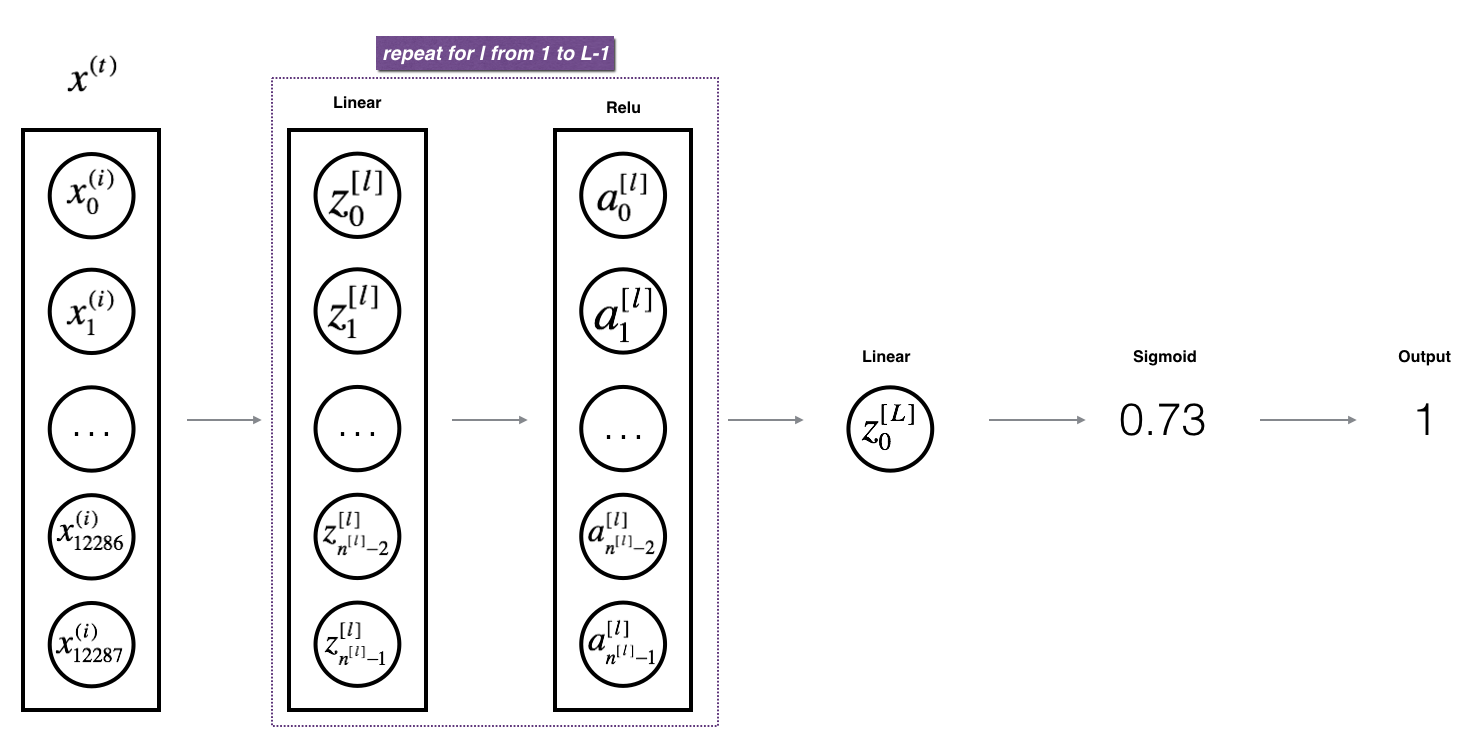
\includegraphics[width=\textwidth]{course1/model_architecture}
\end{center}
\caption{[LINEAR -> RELU] $\times$ (L-1) -> LINEAR -> SIGMOID model}
\label{fig:final_outline}
\end{figure}

{\textbf {Exercise}}: Implement the forward propagation of the above model.

{\textbf {Instruction}}: In the code below, the variable ``AL'' will denote $A^{[L]} = \sigma(Z^{[L]}) = \sigma(W^{[L]} A^{[L-1]} + b^{[L]})$. (This is sometimes also called ``Yhat'', i.e., this is $\hat{Y}$.) 

{\textbf {Tips}}:
\begin{itemize}
\item Use the functions you had previously written 
\item Use a for loop to replicate [LINEAR->RELU] (L-1) times
\item Don't forget to keep track of the caches in the ``caches'' list. To add a new value ``c'' to a ``list'', you can use ``list.append(c)''.
\end{itemize}

\begin{minted}{python}
# GRADED FUNCTION: L_model_forward
def L_model_forward(X, parameters):
    """
    Implement forward propagation for the [LINEAR->RELU]*(L-1)->LINEAR->SIGMOID computation
    
    Arguments:
    X -- data, numpy array of shape (input size, number of examples)
    parameters -- output of initialize_parameters_deep()
    
    Returns:
    AL -- last post-activation value
    caches -- list of caches containing:
                every cache of linear_relu_forward() (there are L-1 of them, indexed from 0 to L-2)
                the cache of linear_sigmoid_forward() (there is one, indexed L-1)
    """

    caches = []
    A = X
    L = len(parameters) // 2 # number of layers in the neural network
    
    # Implement [LINEAR -> RELU]*(L-1). Add "cache" to the "caches" list.
    for l in range(1, L):
        A_prev = A 
        ### START CODE HERE ### (≈ 2 lines of code)
        A, cache = linear_activation_forward(A_prev, parameters['W' + str(l)], parameters['b' + str(l)], activation ="relu")
        caches.append(cache)
        ### END CODE HERE ###
    
    # Implement LINEAR -> SIGMOID. Add "cache" to the "caches" list.
    ### START CODE HERE ### (≈ 2 lines of code)
    AL, cache = linear_activation_forward(A, parameters['W' + str(L)], parameters['b' + str(L)], activation = "sigmoid")
    caches.append(cache)
    ### END CODE HERE ###
    
    assert(AL.shape == (1,X.shape[1]))
            
    return AL, caches
\end{minted}

Great! Now you have a full forward propagation that takes the input X and outputs a row vector $A^{[L]}$ containing your predictions. It also records all intermediate values in ``caches''. Using $A^{[L]}$, you can compute the cost of your predictions.




\subsubsection{Cost function}

Now you will implement forward and backward propagation. You need to compute the cost, because you want to check if your model is actually learning.

{\textbf {Exercise}}: Compute the cross-entropy cost $J$, using the following formula: 
\begin{equation}
\frac{1}{m} \sum\limits_{i = 1}^{m} (y^{(i)}\log\left(a^{[L] (i)}\right) + (1-y^{(i)})\log\left(1- a^{[L](i)}\right)) 
\end{equation}

\begin{minted}{python}
# GRADED FUNCTION: compute_cost
def compute_cost(AL, Y):
    """
    Implement the cost function defined by equation (7).

    Arguments:
    AL -- probability vector corresponding to your label predictions, shape (1, number of examples)
    Y -- true "label" vector (for example: containing 0 if non-cat, 1 if cat), shape (1, number of examples)

    Returns:
    cost -- cross-entropy cost
    """
    
    m = Y.shape[1]

    # Compute loss from aL and y.
    ### START CODE HERE ### (≈ 1 lines of code)
    cost = -(np.dot(Y,np.log(AL.T))+np.dot(1-Y,np.log(1-AL).T))/m
    ### END CODE HERE ###
    
    cost = np.squeeze(cost)      # To make sure your cost's shape is what we expect (e.g. this turns [[17]] into 17).
    assert(cost.shape == ())
    
    return cost
\end{minted}


\subsubsection{Backward propagation module}

Just like with forward propagation, you will implement helper functions for backpropagation. Remember that back propagation is used to calculate the gradient of the loss function with respect to the parameters.

{\textbf {Reminder}}:

\begin{figure}[h]
\begin{center}
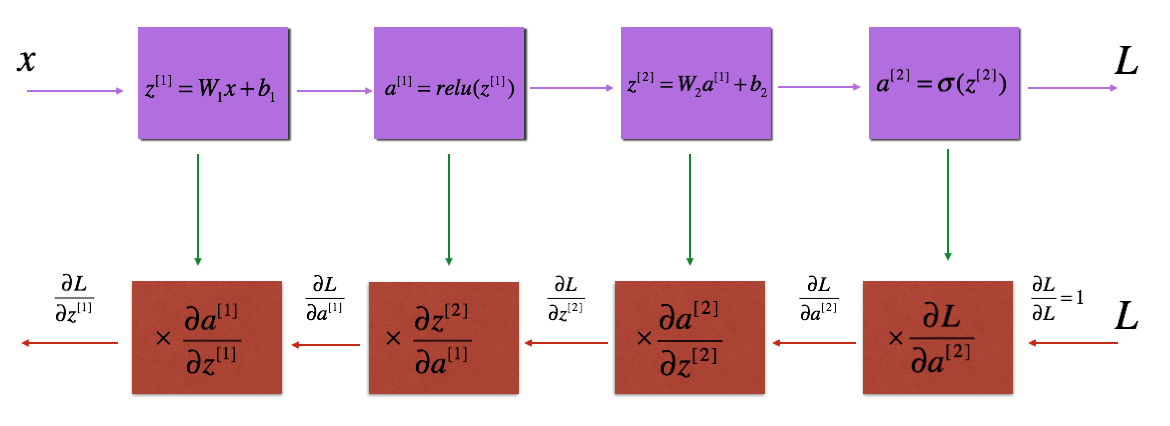
\includegraphics[width=\textwidth]{course1/backprop}
\end{center}
\caption{ Forward and Backward propagation for LINEAR->RELU->LINEAR->SIGMOID. The purple blocks represent the forward propagation, and the red blocks represent the backward propagation.}
\label{fig:backprop}
\end{figure}

Now, similar to forward propagation, you are going to build the backward propagation in three steps:
\begin{itemize}
\item[1] LINEAR backward
\item[2] LINEAR -> ACTIVATION backward where ACTIVATION computes the derivative of either the ReLU or sigmoid activation
\item[3] [LINEAR -> RELU] $\times $ (L-1) -> LINEAR -> SIGMOID backward (whole model)
\end{itemize}



\subsubsubsection{Linear backward}

\begin{figure}[h]
\begin{center}
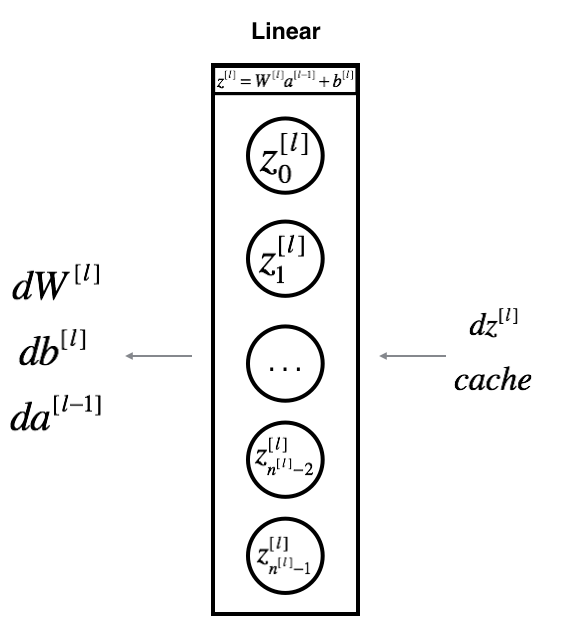
\includegraphics[width=0.34\textwidth]{course1/linearback}
\end{center}
\caption{Linear backward}
\label{fig:linearback}
\end{figure}

For layer $l$, the linear part is: $Z^{[l]} = W^{[l]} A^{[l-1]} + b^{[l]}$ (followed by an activation).

Suppose you have already calculated the derivative $dZ^{[l]} = \frac{\partial \mathcal{L} }{\partial Z^{[l]}}$. You want to get $(dW^{[l]}, db^{[l]} dA^{[l-1]})$.

The three outputs $(dW^{[l]}, db^{[l]}, dA^{[l]})$ are computed using the input $dZ^{[l]}$.Here are the formulas you need:
\begin{align}
dW^{[l]} = \frac{\partial \mathcal{L} }{\partial W^{[l]}} &= \frac{1}{m} dZ^{[l]} A^{[l-1] T} \\
db^{[l]} = \frac{\partial \mathcal{L} }{\partial b^{[l]}} &= \frac{1}{m} \sum_{i = 1}^{m} dZ^{[l](i)}\\
dA^{[l-1]} = \frac{\partial \mathcal{L} }{\partial A^{[l-1]}} &= W^{[l] T} dZ^{[l]} 
\end{align}

{\textbf {Exercise:}} Use the 3 formulas above to implement linear\_backward().

\begin{minted}{python}
# GRADED FUNCTION: linear_backward

def linear_backward(dZ, cache):
    """
    Implement the linear portion of backward propagation for a single layer (layer l)

    Arguments:
    dZ -- Gradient of the cost with respect to the linear output (of current layer l)
    cache -- tuple of values (A_prev, W, b) coming from the forward propagation in the current layer

    Returns:
    dA_prev -- Gradient of the cost with respect to the activation (of the previous layer l-1), same shape as A_prev
    dW -- Gradient of the cost with respect to W (current layer l), same shape as W
    db -- Gradient of the cost with respect to b (current layer l), same shape as b
    """
    A_prev, W, b = cache
    m = A_prev.shape[1]

    ### START CODE HERE ### (≈ 3 lines of code)
    dW = np.dot(dZ,A_prev.T)/m
    db = np.sum(dZ,axis=1,keepdims=True)/m
    dA_prev = np.dot(W.T,dZ)
    ### END CODE HERE ###
    
    assert (dA_prev.shape == A_prev.shape)
    assert (dW.shape == W.shape)
    assert (db.shape == b.shape)
    
    return dA_prev, dW, db
\end{minted}



\subsubsubsection{Linear-Activation backward}

Next, you will create a function that merges the two helper functions: {\textbf {linear\_backward}} and the backward step for the activation {\textbf {linear\_activation\_backward}}. 

To help you implement \emph{linear\_activation\_backward}, we provided two backward functions:
\begin{itemize}
\item {\textbf {sigmoid\_backward}}: Implements the backward propagation for SIGMOID unit. You can call it as follows:
\begin{minted}{python}
dZ = sigmoid_backward(dA, activation_cache)
\end{minted}
\item {\textbf {relu\_backward}}: Implements the backward propagation for RELU unit. You can call it as follows:
\begin{minted}{python}
dZ = relu_backward(dA, activation_cache)
\end{minted}
\end{itemize}

If $g(.)$ is the activation function, \emph{sigmoid\_backward} and \emph{relu\_backward} compute 
\begin{equation}
dZ^{[l]} = dA^{[l]} * g'(Z^{[l]})
\end{equation}

{\textbf {Exercise}}: Implement the backpropagation for the \emph{LINEAR->ACTIVATION} layer.

\begin{minted}{python}
# GRADED FUNCTION: linear_activation_backward
def linear_activation_backward(dA, cache, activation):
    """
    Implement the backward propagation for the LINEAR->ACTIVATION layer.
    
    Arguments:
    dA -- post-activation gradient for current layer l 
    cache -- tuple of values (linear_cache, activation_cache) we store for computing backward propagation efficiently
    activation -- the activation to be used in this layer, stored as a text string: "sigmoid" or "relu"
    
    Returns:
    dA_prev -- Gradient of the cost with respect to the activation (of the previous layer l-1), same shape as A_prev
    dW -- Gradient of the cost with respect to W (current layer l), same shape as W
    db -- Gradient of the cost with respect to b (current layer l), same shape as b
    """
    linear_cache, activation_cache = cache
    
    if activation == "relu":
        ### START CODE HERE ### (≈ 2 lines of code)
        dZ =  relu_backward(dA, activation_cache)
        dA_prev, dW, db = linear_backward(dZ, linear_cache)
        ### END CODE HERE ###
        
    elif activation == "sigmoid":
        ### START CODE HERE ### (≈ 2 lines of code)
        dZ =  sigmoid_backward(dA, activation_cache)
        dA_prev, dW, db = linear_backward(dZ, linear_cache)
        ### END CODE HERE ###
    
    return dA_prev, dW, db
\end{minted}


\subsubsubsection{L-Model Backward}

Now you will implement the backward function for the whole network. Recall that when you implemented the \emph{L\_model\_forward} function, at each iteration, you stored a cache which contains (X,W,b, and z). In the back propagation module, you will use those variables to compute the gradients. Therefore, in the \emph{L\_model\_backward} function, you will iterate through all the hidden layers backward, starting from layer $L$. On each step, you will use the cached values for layer $l$ to backpropagate through layer $l$. Figure \ref{fig: backward} below shows the backward pass. 

\begin{figure}[h]
\begin{center}
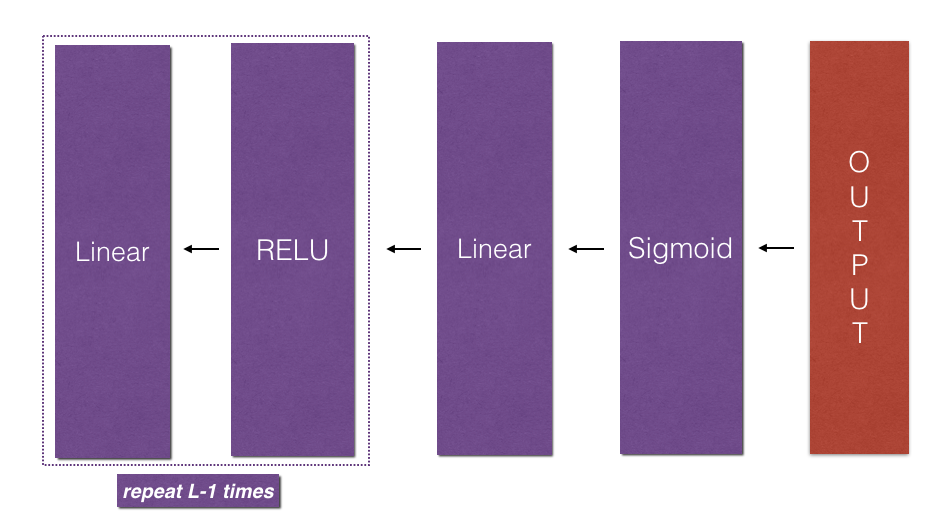
\includegraphics[width=0.8\textwidth]{course1/backward}
\end{center}
\caption{Backward pass}
\label{fig: backward}
\end{figure}


{\textbf {Initializing backpropagation}}:
To backpropagate through this network, we know that the output is, 
$A^{[L]} = \sigma(Z^{[L]})$. Your code thus needs to compute \emph{dAL} $= \frac{\partial \mathcal{L}}{\partial A^{[L]}}$.
To do so, use this formula (derived using calculus which you don't need in-depth knowledge of):
\begin{minted}{python}
dAL = - (np.divide(Y, AL) - np.divide(1 - Y, 1 - AL)) # derivative of cost with respect to AL
\end{minted}

You can then use this post-activation gradient \emph{dAL} to keep going backward. As seen in Figure \ref{fig: backward}, you can now feed in \emph{dAL} into the LINEAR->SIGMOID backward function you implemented (which will use the cached values stored by the L\_model\_forward function). After that, you will have to use a \emph{for} loop to iterate through all the other layers using the LINEAR->RELU backward function. You should store each dA, dW, and db in the grads dictionary. To do so, use this formula : 
\begin{equation}
grads[``dW" + str(l)] = dW^{[l]}
\end{equation}

For example, for $l=3$ this would store $dW^{[l]}$ in \emph{grads[``dW3"]}.

{\textbf {Exercise}}: Implement backpropagation for the \emph{[LINEAR->RELU] $\times$ (L-1) -> LINEAR -> SIGMOID} model.

\begin{minted}{python}
# GRADED FUNCTION: L_model_backward
def L_model_backward(AL, Y, caches):
    """
    Implement the backward propagation for the [LINEAR->RELU] * (L-1) -> LINEAR -> SIGMOID group
    
    Arguments:
    AL -- probability vector, output of the forward propagation (L_model_forward())
    Y -- true "label" vector (containing 0 if non-cat, 1 if cat)
    caches -- list of caches containing:
                every cache of linear_activation_forward() with "relu" (it's caches[l], for l in range(L-1) i.e l = 0...L-2)
                the cache of linear_activation_forward() with "sigmoid" (it's caches[L-1])
    
    Returns:
    grads -- A dictionary with the gradients
             grads["dA" + str(l)] = ... 
             grads["dW" + str(l)] = ...
             grads["db" + str(l)] = ... 
    """
    grads = {}
    L = len(caches) # the number of layers
    m = AL.shape[1]
    Y = Y.reshape(AL.shape) # after this line, Y is the same shape as AL
    
    # Initializing the backpropagation
    ### START CODE HERE ### (1 line of code)
    dAL =  - (np.divide(Y, AL) - np.divide(1 - Y, 1 - AL))
    ### END CODE HERE ###
    
    # Lth layer (SIGMOID -> LINEAR) gradients. Inputs: "AL, Y, caches". Outputs: "grads["dAL"], grads["dWL"], grads["dbL"]
    ### START CODE HERE ### (approx. 2 lines)
    current_cache = caches[L-1]
    grads["dA" + str(L)], grads["dW" + str(L)], grads["db" + str(L)] =  linear_activation_backward(dAL, current_cache, "sigmoid")
    ### END CODE HERE ###
    
    for l in reversed(range(L-1)):
        # lth layer: (RELU -> LINEAR) gradients.
        # Inputs: "grads["dA" + str(l + 2)], caches". Outputs: "grads["dA" + str(l + 1)] , grads["dW" + str(l + 1)] , grads["db" + str(l + 1)] 
        ### START CODE HERE ### (approx. 5 lines)
        current_cache = caches[l]
        dA_prev_temp, dW_temp, db_temp = linear_activation_backward(grads["dA" + str(l+2)], current_cache, "relu")
        grads["dA" + str(l + 1)] = dA_prev_temp
        grads["dW" + str(l + 1)] = dW_temp
        grads["db" + str(l + 1)] = db_temp
        ### END CODE HERE ###

    return grads
\end{minted}


\subsubsubsection{Update Parameters}

In this section you will update the parameters of the model, using gradient descent: 
\begin{align}
W^{[l]} &= W^{[l]} - \alpha \text{ } dW^{[l]} \\
b^{[l]} &= b^{[l]} - \alpha \text{ } db^{[l]}
\end{align}
where $\alpha$ is the learning rate. After computing the updated parameters, store them in the parameters dictionary. 

{\textbf {Exercise}}: Implement ``update\_parameters()'' to update your parameters using gradient descent.

{\textbf {Instructions}}:
Update parameters using gradient descent on every $W^{[l]}$ and $b^{[l]}$ for $l = 1, 2, ..., L$. 
\begin{minted}{python}
# GRADED FUNCTION: update_parameters
def update_parameters(parameters, grads, learning_rate):
    """
    Update parameters using gradient descent
    
    Arguments:
    parameters -- python dictionary containing your parameters 
    grads -- python dictionary containing your gradients, output of L_model_backward
    
    Returns:
    parameters -- python dictionary containing your updated parameters 
                  parameters["W" + str(l)] = ... 
                  parameters["b" + str(l)] = ...
    """
    
    L = len(parameters) // 2 # number of layers in the neural network

    # Update rule for each parameter. Use a for loop.
    ### START CODE HERE ### (≈ 3 lines of code)
    for l in range(L):
        parameters["W" + str(l+1)] =  parameters["W" + str(l+1)] - learning_rate * grads["dW" + str(l + 1)]
        parameters["b" + str(l+1)] = parameters["b" + str(l+1)] - learning_rate * grads["db" + str(l + 1)]
    ### END CODE HERE ###
    return parameters
\end{minted}




\subsubsubsection{Conclusion}

Congrats on implementing all the functions required for building a deep neural network!

We know it was a long assignment but going forward it will only get better. The next part of the assignment is easier.

In the next assignment you will put all these together to build two models:
\begin{itemize}
\item A two-layer neural network
\item An L-layer neural network
\end{itemize}

You will in fact use these models to classify cat vs non-cat images!



\clearpage
\subsubsection{Code of Deep Neural Network}
\begin{minted}{python}
import numpy as np
import h5py
import matplotlib.pyplot as plt
from testCases_v3 import *
from dnn_utils_v2 import sigmoid, sigmoid_backward, relu, relu_backward

#matplotlib inline
plt.rcParams['figure.figsize'] = (5.0, 4.0) # set default size of plots
plt.rcParams['image.interpolation'] = 'nearest'
plt.rcParams['image.cmap'] = 'gray'


# GRADED FUNCTION: initialize_parameters
def initialize_parameters(n_x, n_h, n_y):
    """
    Argument:
    n_x -- size of the input layer
    n_h -- size of the hidden layer
    n_y -- size of the output layer
    
    Returns:
    parameters -- python dictionary containing your parameters:
                    W1 -- weight matrix of shape (n_h, n_x)
                    b1 -- bias vector of shape (n_h, 1)
                    W2 -- weight matrix of shape (n_y, n_h)
                    b2 -- bias vector of shape (n_y, 1)
    """
    
    np.random.seed(1)
    
    W1 = np.random.randn(n_h, n_x)*0.01
    b1 = np.zeros((n_h, 1))
    W2 = np.random.randn(n_y, n_h)*0.01
    b2 = np.zeros((n_y, 1))
    
    assert(W1.shape == (n_h, n_x))
    assert(b1.shape == (n_h, 1))
    assert(W2.shape == (n_y, n_h))
    assert(b2.shape == (n_y, 1))
    
    parameters = {"W1": W1,
                  "b1": b1,
                  "W2": W2,
                  "b2": b2}
    
    return parameters


# GRADED FUNCTION: initialize_parameters_deep
def initialize_parameters_deep(layer_dims):
    """
    Arguments:
    layer_dims -- python array (list) containing the dimensions of each layer in our network
    
    Returns:
    parameters -- python dictionary containing your parameters "W1", "b1", ..., "WL", "bL":
                    Wl -- weight matrix of shape (layer_dims[l], layer_dims[l-1])
                    bl -- bias vector of shape (layer_dims[l], 1)
    """
    
    np.random.seed(3)
    parameters = {}
    L = len(layer_dims)            # number of layers in the network

    for l in range(1, L):
        parameters['W' + str(l)] = np.random.randn(layer_dims[l], layer_dims[l-1]) * 0.01
        parameters['b' + str(l)] = np.zeros((layer_dims[l], 1))
        
        assert(parameters['W' + str(l)].shape == (layer_dims[l], layer_dims[l-1]))
        assert(parameters['b' + str(l)].shape == (layer_dims[l], 1))
       
    return parameters


# GRADED FUNCTION: linear_forward
def linear_forward(A, W, b):
    """
    Implement the linear part of a layer's forward propagation.

    Arguments:
    A -- activations from previous layer (or input data): (size of previous layer, number of examples)
    W -- weights matrix: numpy array of shape (size of current layer, size of previous layer)
    b -- bias vector, numpy array of shape (size of the current layer, 1)

    Returns:
    Z -- the input of the activation function, also called pre-activation parameter 
    cache -- a python dictionary containing "A", "W" and "b" ; stored for computing the backward pass efficiently
    """
    
    Z = np.dot(W,A)+b
    
    assert(Z.shape == (W.shape[0], A.shape[1]))
    cache = (A, W, b)
    
    return Z, cache


def linear_activation_forward(A_prev, W, b, activation):
    """
    Implement the forward propagation for the LINEAR->ACTIVATION layer

    Arguments:
    A_prev -- activations from previous layer (or input data): (size of previous layer, number of examples)
    W -- weights matrix: numpy array of shape (size of current layer, size of previous layer)
    b -- bias vector, numpy array of shape (size of the current layer, 1)
    activation -- the activation to be used in this layer, stored as a text string: "sigmoid" or "relu"

    Returns:
    A -- the output of the activation function, also called the post-activation value 
    cache -- a python dictionary containing "linear_cache" and "activation_cache";
             stored for computing the backward pass efficiently
    """
    
    if activation == "sigmoid":
        # Inputs: "A_prev, W, b". Outputs: "A, activation_cache".
        Z, linear_cache = linear_forward(A_prev, W, b)
        A, activation_cache = sigmoid(Z)
    
    elif activation == "relu":
        # Inputs: "A_prev, W, b". Outputs: "A, activation_cache".
        Z, linear_cache = linear_forward(A_prev, W, b)
        A, activation_cache = relu(Z)
    
    assert (A.shape == (W.shape[0], A_prev.shape[1]))
    cache = (linear_cache, activation_cache)

    return A, cache


# GRADED FUNCTION: L_model_forward
def L_model_forward(X, parameters):
    """
    Implement forward propagation for the [LINEAR->RELU]*(L-1)->LINEAR->SIGMOID computation
    
    Arguments:
    X -- data, numpy array of shape (input size, number of examples)
    parameters -- output of initialize_parameters_deep()
    
    Returns:
    AL -- last post-activation value
    caches -- list of caches containing:
                every cache of linear_relu_forward() (there are L-1 of them, indexed from 0 to L-2)
                the cache of linear_sigmoid_forward() (there is one, indexed L-1)
    """

    caches = []
    A = X
    L = len(parameters) // 2     # number of layers in the neural network
    
    # Implement [LINEAR -> RELU]*(L-1). Add "cache" to the "caches" list.
    for l in range(1, L):
        A_prev = A 
        A, cache = linear_activation_forward(A_prev, parameters['W' + str(l)], parameters['b' + str(l)], activation ="relu")
        caches.append(cache)
    
    # Implement LINEAR -> SIGMOID. Add "cache" to the "caches" list.
    AL, cache = linear_activation_forward(A, parameters['W' + str(L)], parameters['b' + str(L)], activation = "sigmoid")
    caches.append(cache)
    
    assert(AL.shape == (1,X.shape[1]))
            
    return AL, caches


# GRADED FUNCTION: compute_cost
def compute_cost(AL, Y):
    """
    Implement the cost function defined by equation (7).

    Arguments:
    AL -- probability vector corresponding to your label predictions, shape (1, number of examples)
    Y -- true "label" vector (for example: containing 0 if non-cat, 1 if cat), shape (1, number of examples)

    Returns:
    cost -- cross-entropy cost
    """
    
    m = Y.shape[1]
    # Compute loss from aL and y.
    cost = -(np.dot(Y,np.log(AL.T))+np.dot(1-Y,np.log(1-AL).T))/m
    
    cost = np.squeeze(cost)      # To make sure your cost's shape is what we expect (e.g. this turns [[17]] into 17).
    assert(cost.shape == ())
    
    return cost


# GRADED FUNCTION: linear_backward
def linear_backward(dZ, cache):
    """
    Implement the linear portion of backward propagation for a single layer (layer l)

    Arguments:
    dZ -- Gradient of the cost with respect to the linear output (of current layer l)
    cache -- tuple of values (A_prev, W, b) coming from the forward propagation in the current layer

    Returns:
    dA_prev -- Gradient of the cost with respect to the activation (of the previous layer l-1), same shape as A_prev
    dW -- Gradient of the cost with respect to W (current layer l), same shape as W
    db -- Gradient of the cost with respect to b (current layer l), same shape as b
    """
    A_prev, W, b = cache
    m = A_prev.shape[1]

    dW = np.dot(dZ,A_prev.T)/m
    db = np.sum(dZ,axis=1,keepdims=True)/m
    dA_prev = np.dot(W.T,dZ)
    
    assert (dA_prev.shape == A_prev.shape)
    assert (dW.shape == W.shape)
    assert (db.shape == b.shape)
    
    return dA_prev, dW, db


# GRADED FUNCTION: linear_activation_backward

def linear_activation_backward(dA, cache, activation):
    """
    Implement the backward propagation for the LINEAR->ACTIVATION layer.
    
    Arguments:
    dA -- post-activation gradient for current layer l 
    cache -- tuple of values (linear_cache, activation_cache) we store for computing backward propagation efficiently
    activation -- the activation to be used in this layer, stored as a text string: "sigmoid" or "relu"
    
    Returns:
    dA_prev -- Gradient of the cost with respect to the activation (of the previous layer l-1), same shape as A_prev
    dW -- Gradient of the cost with respect to W (current layer l), same shape as W
    db -- Gradient of the cost with respect to b (current layer l), same shape as b
    """
    linear_cache, activation_cache = cache
    
    if activation == "relu":
        dZ =  relu_backward(dA, activation_cache)
        dA_prev, dW, db = linear_backward(dZ, linear_cache)
        
    elif activation == "sigmoid":
        dZ =  sigmoid_backward(dA, activation_cache)
        dA_prev, dW, db = linear_backward(dZ, linear_cache)
    
    return dA_prev, dW, db


# GRADED FUNCTION: L_model_backward
def L_model_backward(AL, Y, caches):
    """
    Implement the backward propagation for the [LINEAR->RELU] * (L-1) -> LINEAR -> SIGMOID group
    
    Arguments:
    AL -- probability vector, output of the forward propagation (L_model_forward())
    Y -- true "label" vector (containing 0 if non-cat, 1 if cat)
    caches -- list of caches containing:
                every cache of linear_activation_forward() with "relu" (it's caches[l], for l in range(L-1) i.e l = 0...L-2)
                the cache of linear_activation_forward() with "sigmoid" (it's caches[L-1])
    
    Returns:
    grads -- A dictionary with the gradients
             grads["dA" + str(l)] = ... 
             grads["dW" + str(l)] = ...
             grads["db" + str(l)] = ... 
    """
    grads = {}
    L = len(caches) # the number of layers
    m = AL.shape[1]
    Y = Y.reshape(AL.shape) # after this line, Y is the same shape as AL
    
    # Initializing the backpropagation
    dAL =  - (np.divide(Y, AL) - np.divide(1 - Y, 1 - AL))
    
    # Lth layer (SIGMOID -> LINEAR) gradients. Inputs: "AL, Y, caches". Outputs: "grads["dAL"], grads["dWL"], grads["dbL"]
    current_cache = caches[L-1]
    grads["dA" + str(L)], grads["dW" + str(L)], grads["db" + str(L)] =  linear_activation_backward(dAL, current_cache, "sigmoid")
    
    for l in reversed(range(L-1)):
        # lth layer: (RELU -> LINEAR) gradients.
        # Inputs: "grads["dA" + str(l + 2)], caches". Outputs: "grads["dA" + str(l + 1)] , grads["dW" + str(l + 1)] , grads["db" + str(l + 1)] 
        current_cache = caches[l]
        dA_prev_temp, dW_temp, db_temp = linear_activation_backward(grads["dA" + str(l+2)], current_cache, "relu")
        grads["dA" + str(l + 1)] = dA_prev_temp
        grads["dW" + str(l + 1)] = dW_temp
        grads["db" + str(l + 1)] = db_temp

    return grads

# GRADED FUNCTION: update_parameters

def update_parameters(parameters, grads, learning_rate):
    """
    Update parameters using gradient descent
    
    Arguments:
    parameters -- python dictionary containing your parameters 
    grads -- python dictionary containing your gradients, output of L_model_backward
    
    Returns:
    parameters -- python dictionary containing your updated parameters 
                  parameters["W" + str(l)] = ... 
                  parameters["b" + str(l)] = ...
    """
    
    L = len(parameters) // 2 # number of layers in the neural network
    # Update rule for each parameter. Use a for loop.
    for l in range(L):
        parameters["W" + str(l+1)] =  parameters["W" + str(l+1)] - learning_rate * grads["dW" + str(l + 1)]
        parameters["b" + str(l+1)] = parameters["b" + str(l+1)] - learning_rate * grads["db" + str(l + 1)]
    return parameters

\end{minted}
\clearpage
\subsection{Deep Neural Network for Image Classification: Application}

Congratulations! Welcome to the fourth programming exercise of the deep learning specialization. You will now use everything you have learned to build a deep neural network that classifies {\textbf{cat vs. non-cat images}}.

\begin{figure}[h]
\begin{center}

\includegraphics[width=\textwidth]{course1/cat_2}
\end{center}
\end{figure}

In the second exercise, you used logistic regression to build cat vs. non-cat images and got a 68\% accuracy. Your algorithm will now give you an 80\% accuracy! you will see an improvement in accuracy relative to your previous logistic regression implementation. By completing this assignment, you will:
\begin{itemize}
\item Learn how to use all the helper functions you built in the previous assignment to build a model of any structure you want.
\item Experiment with different model architectures and see how each one behaves.
\item Recognize that it is always easier to build your helper functions before attempting to build a neural network from scratch.
\end{itemize}

This assignment prepares you well for the next course which dives deep into the techniques and strategies for parameters tuning and initializations. When you finish this, you will have finished the last programming assignment of Week 4, and also the last programming assignment of this course! Take your time to complete this assignment and make sure you get the expected outputs when working through the different exercises. In some code blocks, you will find a "\#GRADED FUNCTION: functionName" comment. Please do not modify it. After you are done, submit your work and check your results. You need to score 70\% to pass. Good luck :) !


{\textbf {After this assignment you will be able to}}: {\color{red}Build and apply a deep neural network to supervised learning}.
Let's get started!


\subsubsection{Packages}

Let's first import all the packages that you will need during this assignment.
\begin{itemize}
\item \href{www.numpy.org}{numpy} is the fundamental package for scientific computing with Python.
\item \href{http://www.h5py.org}{h5py} is a common package to interact with a dataset that is stored on an H5 file.
\item \href{http://matplotlib.org}{matplotlib} is a famous library to plot graphs in Python.
\item \href{http://www.pythonware.com/products/pil/}{PIL} and \href{https://www.scipy.org/}{scipy} are used here to test your model with your own picture at the end.
\item dnn\_app\_utils provides the functions implemented in the "Building your Deep Neural Network: Step by Step" assignment to this notebook.
\item np.random.seed(1) is used to keep all the random function calls consistent. It will help us grade your work.
\end{itemize}


\begin{minted}{python}
import time
import numpy as np
import h5py
import matplotlib.pyplot as plt
import scipy
from PIL import Image
from scipy import ndimage
from dnn_app_utils_v2 import *

#matplotlib inline
plt.rcParams['figure.figsize'] = (5.0, 4.0) # set default size of plots
plt.rcParams['image.interpolation'] = 'nearest'
plt.rcParams['image.cmap'] = 'gray'

#load_ext autoreload
#autoreload 2

np.random.seed(1)
\end{minted}





\subsubsection{Dataset}

You will use the same ``Cat vs non-Cat'' dataset as in ``Logistic Regression as a Neural Network'' (Assignment 2). The model you had built had 70\% test accuracy on classifying cats vs non-cats images. Hopefully, your new model will perform a better!

{\textbf {Problem Statement}}: You are given a dataset (``data.h5") containing:
\begin{itemize}
\item a training set of m\_train images labelled as cat (1) or non-cat (0)
\item a test set of m\_test images labelled as cat and non-cat
\item each image is of shape (num\_px, num\_px, 3) where 3 is for the 3 channels (RGB).
\end{itemize}

Let's get more familiar with the dataset. Load the data by running the cell below.
\begin{minted}{python}
train_x_orig, train_y, test_x_orig, test_y, classes = load_data()
\end{minted}

The following code will show you an image in the dataset. Feel free to change the index and re-run the cell multiple times to see other images.
\begin{minted}{python}
# Example of a picture
index = 10
plt.imshow(train_x_orig[index])
print ("y = " + str(train_y[0,index]) + ". It's a " + classes[train_y[0,index]].decode("utf-8") +  " picture.")
\end{minted}

\begin{minted}{python}
# Explore your dataset 
m_train = train_x_orig.shape[0]
m_test =  test_x_orig.shape[0]
num_px = train_x_orig.shape[1]
\end{minted}

As usual, you reshape and standardize the images before feeding them to the network. The code is given below.
\begin{figure}[h]
\begin{center}
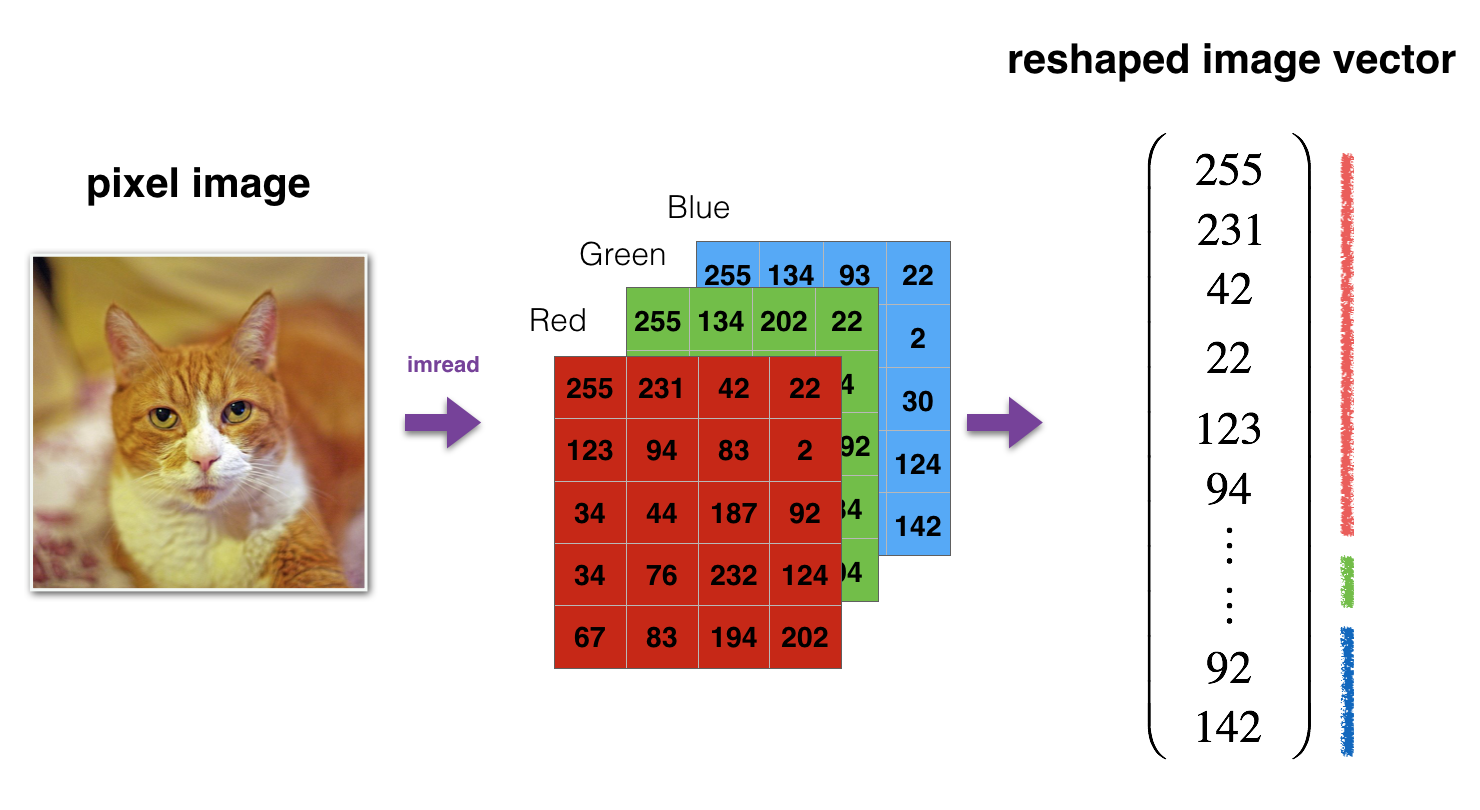
\includegraphics[width=0.9\textwidth]{course1/Image_to_vector_conversion}
\caption{Image to vector conversion}
\end{center}
\end{figure}

12288  equals 64$\times$64$\times$3 which is the size of one reshaped image vector.


\subsubsection{Architecture of your model}

Now that you are familiar with the dataset, it is time to build a deep neural network to distinguish cat images from non-cat images.

You will build two different models:
\begin{itemize}
\item A 2-layer neural network
\item An L-layer deep neural network
\end{itemize}

You will then compare the performance of these models, and also try out different values for $L$. 

Let's look at the two architectures.

\subsubsubsection{2-layer neural network}

\begin{figure}[h]
\begin{center}
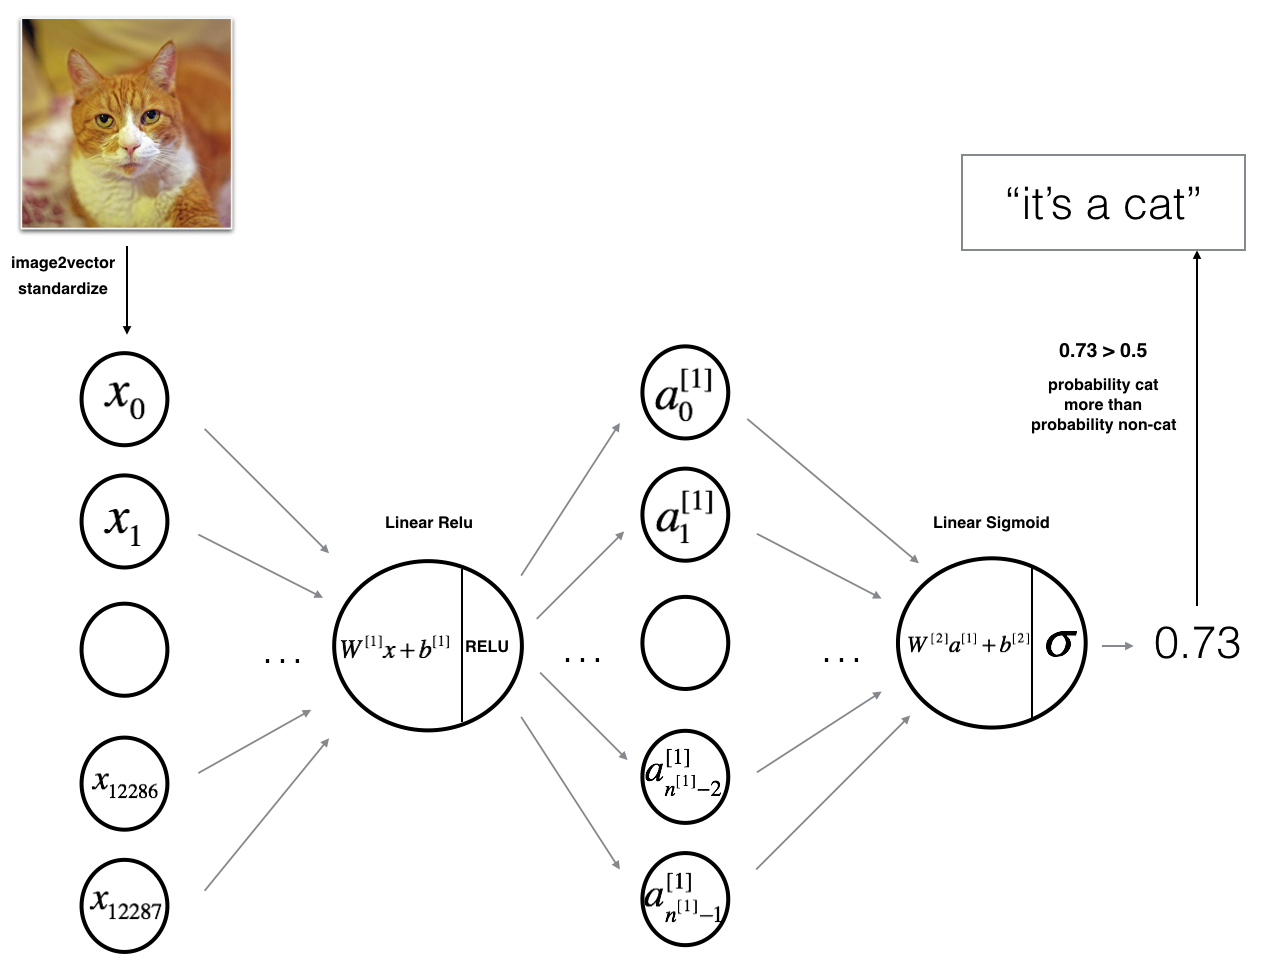
\includegraphics[width=0.65\textwidth]{course1/2layerNN}
\caption{2-layer neural network}
\label{2layerNN}
\end{center}
\end{figure}

The model can be summarized as: \emph{INPUT -> LINEAR -> RELU -> LINEAR -> SIGMOID -> OUTPUT}. Detailed Architecture of figure \ref{2layerNN}:
\begin{itemize}
\item The input is a (64,64,3) image which is flattened to a vector of size $(12288,1)$. 
\item The corresponding vector: $[x_0,x_1,...,x_{12287}]^T$ is then multiplied by the weight matrix $W^{[1]}$ of size $(n^{[1]}, 12288)$.
\item You then add a bias term and take its relu to get the following vector: $[a_0^{[1]}, a_1^{[1]},..., a_{n^{[1]}-1}^{[1]}]^T$.
\item You then repeat the same process.
\item You multiply the resulting vector by $W^{[2]}$ and add your intercept (bias). 
\item Finally, you take the sigmoid of the result. If it is greater than 0.5, you classify it to be a cat.
\end{itemize}



\subsubsubsection{L-layer deep neural network}

It is hard to represent an L-layer deep neural network with the above representation. However, figure \ref{LlayerNN} is a simplified network representation:
\begin{figure}[h]
\begin{center}
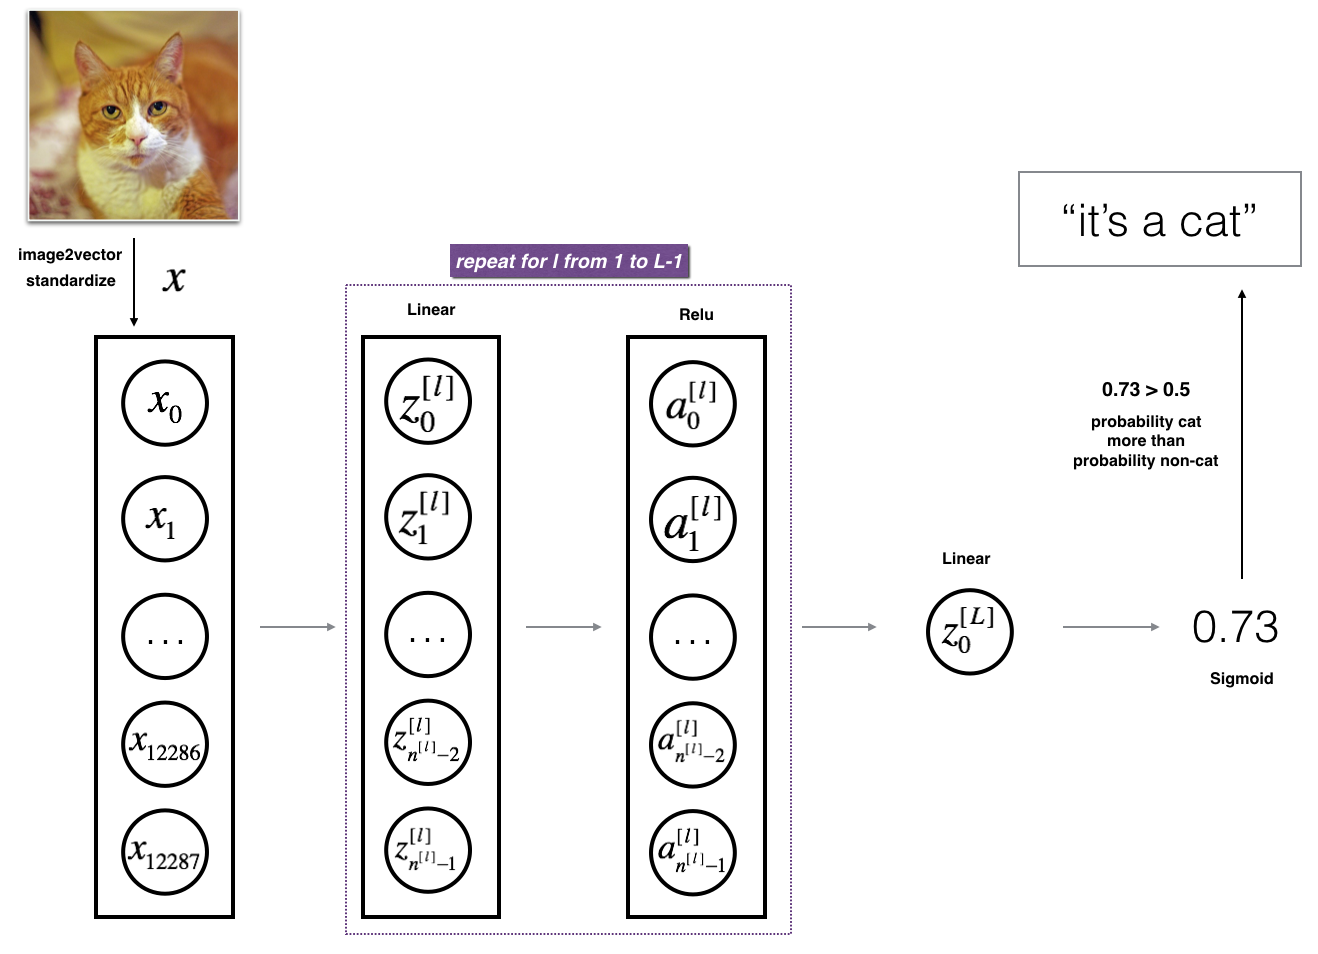
\includegraphics[width=0.65\textwidth]{course1/LlayerNN}
\caption{ L-layer neural network}
\label{LlayerNN}
\end{center}
\end{figure}


The model can be summarized as: \emph{[LINEAR -> RELU]  $\times$  (L-1) -> LINEAR -> SIGMOID}. Detailed Architecture of figure \ref{LlayerNN}:
\begin{itemize}
\item The input is a (64,64,3) image which is flattened to a vector of size (12288,1).
\item The corresponding vector: $[x_0,x_1,...,x_{12287}]^T$ is then multiplied by the weight matrix $W^{[1]}$ and then you add the intercept $b^{[1]}$. The result is called the linear unit.
\item Next, you take the relu of the linear unit. This process could be repeated several times for each $(W^{[l]}, b^{[l]})$ depending on the model architecture.
\item Finally, you take the sigmoid of the final linear unit. If it is greater than 0.5, you classify it to be a cat.
\end{itemize}



\subsubsubsection{General methodology}

As usual you will follow the Deep Learning methodology to build the model:
\begin{itemize}
\item[1.] Initialize parameters / Define hyperparameters
\item[2.] Loop for num\_iterations:
\begin{itemize}
\item[a.] Forward propagation
\item[b.] Compute cost function
\item[c.] Backward propagation
\item[d.] Update parameters (using parameters, and grads from backprop) 
\end{itemize}
\item[3.] Use trained parameters to predict labels
\end{itemize}

Let's now implement those two models!



\subsubsection{Two-layer neural network}

{\textbf {Question}}: Use the helper functions you have implemented in the previous assignment to build a 2-layer neural network with the following structure: \emph{LINEAR -> RELU -> LINEAR -> SIGMOID}. The functions you may need and their inputs are:
\begin{minted}{python}
def initialize_parameters(n_x, n_h, n_y):
    ...
    return parameters 
def linear_activation_forward(A_prev, W, b, activation):
    ...
    return A, cache
def compute_cost(AL, Y):
    ...
    return cost
def linear_activation_backward(dA, cache, activation):
    ...
    return dA_prev, dW, db
def update_parameters(parameters, grads, learning_rate):
    ...
    return parameters
\end{minted}

The whole code is as follows:

\begin{minted}{python}
### CONSTANTS DEFINING THE MODEL ####
n_x = 12288     # num_px * num_px * 3
n_h = 7
n_y = 1
layers_dims = (n_x, n_h, n_y)


# GRADED FUNCTION: two_layer_model
def two_layer_model(X, Y, layers_dims, learning_rate = 0.0075, num_iterations = 3000, print_cost=False):
    """
    Implements a two-layer neural network: LINEAR->RELU->LINEAR->SIGMOID.
    
    Arguments:
    X -- input data, of shape (n_x, number of examples)
    Y -- true "label" vector (containing 0 if cat, 1 if non-cat), of shape (1, number of examples)
    layers_dims -- dimensions of the layers (n_x, n_h, n_y)
    num_iterations -- number of iterations of the optimization loop
    learning_rate -- learning rate of the gradient descent update rule
    print_cost -- If set to True, this will print the cost every 100 iterations 
    
    Returns:
    parameters -- a dictionary containing W1, W2, b1, and b2
    """
    
    np.random.seed(1)
    grads = {}
    costs = []                              # to keep track of the cost
    m = X.shape[1]                           # number of examples
    (n_x, n_h, n_y) = layers_dims
    
    # Initialize parameters dictionary, by calling one of the functions you'd previously implemented
    ### START CODE HERE ### (≈ 1 line of code)
    parameters =initialize_parameters(n_x, n_h, n_y)
    ### END CODE HERE ###
    
    # Get W1, b1, W2 and b2 from the dictionary parameters.
    W1 = parameters["W1"]
    b1 = parameters["b1"]
    W2 = parameters["W2"]
    b2 = parameters["b2"]
    
    # Loop (gradient descent)

    for i in range(0, num_iterations):

        # Forward propagation: LINEAR -> RELU -> LINEAR -> SIGMOID. Inputs: "X, W1, b1". Output: "A1, cache1, A2, cache2".
        ### START CODE HERE ### (≈ 2 lines of code)
        A1, cache1 = linear_activation_forward(X, W1, b1, "relu")
        A2, cache2 = linear_activation_forward(A1, W2, b2, "sigmoid")
        ### END CODE HERE ###
        
        # Compute cost
        ### START CODE HERE ### (≈ 1 line of code)
        cost =  compute_cost(A2, Y)
        ### END CODE HERE ###
        
        # Initializing backward propagation
        dA2 = - (np.divide(Y, A2) - np.divide(1 - Y, 1 - A2))
        
        # Backward propagation. Inputs: "dA2, cache2, cache1". Outputs: "dA1, dW2, db2; also dA0 (not used), dW1, db1".
        ### START CODE HERE ### (≈ 2 lines of code)
        dA1, dW2, db2 = linear_activation_backward(dA2, cache2, "sigmoid")
        dA0, dW1, db1 = linear_activation_backward(dA1, cache1, "relu")
        ### END CODE HERE ###
        
        # Set grads['dWl'] to dW1, grads['db1'] to db1, grads['dW2'] to dW2, grads['db2'] to db2
        grads['dW1'] = dW1
        grads['db1'] = db1
        grads['dW2'] = dW2
        grads['db2'] = db2
        
        # Update parameters.
        ### START CODE HERE ### (approx. 1 line of code)
        parameters = update_parameters(parameters, grads, learning_rate)
        ### END CODE HERE ###

        # Retrieve W1, b1, W2, b2 from parameters
        W1 = parameters["W1"]
        b1 = parameters["b1"]
        W2 = parameters["W2"]
        b2 = parameters["b2"]
        
        # Print the cost every 100 training example
        if print_cost and i % 100 == 0:
            print("Cost after iteration {}: {}".format(i, np.squeeze(cost)))
        if print_cost and i % 100 == 0:
            costs.append(cost)
       
    # plot the cost

    plt.plot(np.squeeze(costs))
    plt.ylabel('cost')
    plt.xlabel('iterations (per tens)')
    plt.title("Learning rate =" + str(learning_rate))
    plt.show()
    
    return parameters
\end{minted}

\begin{minted}{python}
#input
parameters = two_layer_model(train_x, train_y, layers_dims = (n_x, n_h, n_y), num_iterations = 2500, print_cost=True)

#output
Cost after iteration 0: 0.693049735659989
Cost after iteration 100: 0.6464320953428849
Cost after iteration 200: 0.6325140647912678
......
Cost after iteration 2400: 0.048554785628770226
\end{minted}
\begin{figure}[h]
\begin{center}
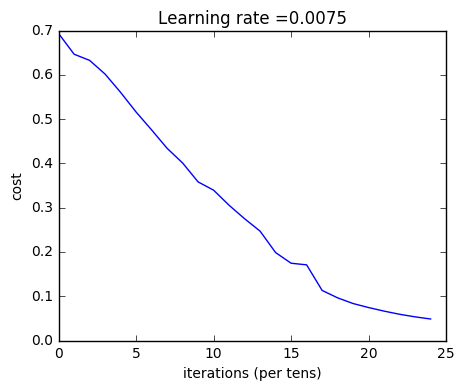
\includegraphics[width=0.6\textwidth]{course1/two_layer_model_result}
\caption{cost}
\label{two_layer_model_result}
\end{center}
\end{figure}


Now, you can use the trained parameters to classify images from the dataset. To see your predictions on the training and test sets, run the code below.
\begin{minted}{python}
predictions_train = predict(train_x, train_y, parameters)
#output
Accuracy: 1.0

predictions_test = predict(test_x, test_y, parameters)
#output
Accuracy: 0.72
\end{minted}

{\textbf {Note}}: You may notice that running the model on fewer iterations (say 1500) gives better accuracy on the test set. This is called {\color{red} \textbf {``early stopping''}} and we will talk about it in the next course. Early stopping is a way to prevent overfitting. 

Congratulations! It seems that your 2-layer neural network has better performance (72\%) than the logistic regression implementation (70\%, \hyperref[sec:logistic_regression]{assignment week 2 }). Let's see if you can do even better with an $L$-layer model.



\subsubsection{L-layer Neural Network}

{\textbf {Question}}: Use the helper functions you have implemented previously to build an $L$-layer neural network with the following structure: \emph{[LINEAR -> RELU]$\times$(L-1) -> LINEAR -> SIGMOID}. The functions you may need and their inputs are:
\begin{minted}{python}
def initialize_parameters_deep(layer_dims):
    ...
    return parameters 
def L_model_forward(X, parameters):
    ...
    return AL, caches
def compute_cost(AL, Y):
    ...
    return cost
def L_model_backward(AL, Y, caches):
    ...
    return grads
def update_parameters(parameters, grads, learning_rate):
    ...
    return parameters
\end{minted}

The whole code is as follows:
\begin{minted}{python}
### CONSTANTS ###
layers_dims = [12288, 20, 7, 5, 1] #  5-layer model

# GRADED FUNCTION: L_layer_model
def L_layer_model(X, Y, layers_dims, learning_rate = 0.0075, num_iterations = 3000, print_cost=False):#lr was 0.009
    """
    Implements a L-layer neural network: [LINEAR->RELU]*(L-1)->LINEAR->SIGMOID.
    
    Arguments:
    X -- data, numpy array of shape (number of examples, num_px * num_px * 3)
    Y -- true "label" vector (containing 0 if cat, 1 if non-cat), of shape (1, number of examples)
    layers_dims -- list containing the input size and each layer size, of length (number of layers + 1).
    learning_rate -- learning rate of the gradient descent update rule
    num_iterations -- number of iterations of the optimization loop
    print_cost -- if True, it prints the cost every 100 steps
    
    Returns:
    parameters -- parameters learnt by the model. They can then be used to predict.
    """

    np.random.seed(1)
    costs = []                         # keep track of cost
    
    # Parameters initialization.
    ### START CODE HERE ###
    parameters = initialize_parameters_deep(layers_dims)
    ### END CODE HERE ###
    
    # Loop (gradient descent)
    for i in range(0, num_iterations):

        # Forward propagation: [LINEAR -> RELU]*(L-1) -> LINEAR -> SIGMOID.
        ### START CODE HERE ### (≈ 1 line of code)
        AL, caches =  L_model_forward(X, parameters)
        ### END CODE HERE ###
        
        # Compute cost.
        ### START CODE HERE ### (≈ 1 line of code)
        cost =  compute_cost(AL, Y)
        ### END CODE HERE ###
    
        # Backward propagation.
        ### START CODE HERE ### (≈ 1 line of code)
        grads =  L_model_backward(AL, Y, caches)
        ### END CODE HERE ###
 
        # Update parameters.
        ### START CODE HERE ### (≈ 1 line of code)
        parameters =  update_parameters(parameters, grads, learning_rate)
        ### END CODE HERE ###
                
        # Print the cost every 100 training example
        if print_cost and i % 100 == 0:
            print ("Cost after iteration %i: %f" %(i, cost))
        if print_cost and i % 100 == 0:
            costs.append(cost)
            
    # plot the cost
    plt.plot(np.squeeze(costs))
    plt.ylabel('cost')
    plt.xlabel('iterations (per tens)')
    plt.title("Learning rate =" + str(learning_rate))
    plt.show()
    
    return parameters
\end{minted}


\begin{minted}{python}
#input
parameters = L_layer_model(train_x, train_y, layers_dims, num_iterations = 2500, print_cost = True)

#output
Cost after iteration 0: 0.771749
Cost after iteration 100: 0.672053
Cost after iteration 200: 0.648263
......
Cost after iteration 2400: 0.092878
\end{minted}
\begin{figure}[h]
\begin{center}
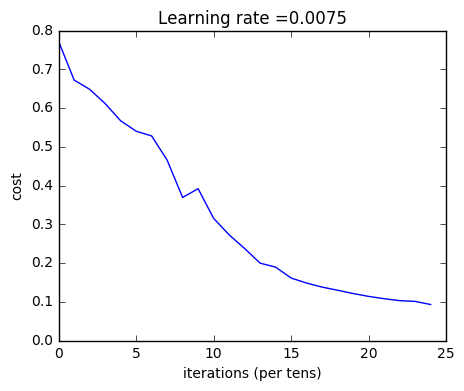
\includegraphics[width=0.6\textwidth]{course1/L_layer_model_result}
\caption{cost}
\label{L_layer_model_result}
\end{center}
\end{figure}

Now, you can use the trained parameters to classify images from the dataset. To see your predictions on the training and test sets, run the code below.
\begin{minted}{python}
pred_train = predict(train_x, train_y, parameters)
#output
Accuracy: 0.985645933014

pred_test = predict(test_x, test_y, parameters)
#output
Accuracy: 0.8
\end{minted}


Congrats! It seems that your 5-layer neural network has better performance (80\%) than your 2-layer neural network (72\%) on the same test set.

This is good performance for this task. Nice job!

Though in the next course on "Improving deep neural networks" you will learn how to obtain even higher accuracy by systematically searching for better hyperparameters (learning\_rate, layers\_dims, num\_iterations, and others you'll also learn in the next course).



\subsubsection{Results Analysis}

First, let's take a look at some images the L-layer model labeled incorrectly. This will show a few mislabeled images.
\begin{minted}{python}
print_mislabeled_images(classes, test_x, test_y, pred_test)
\end{minted}

\begin{figure}[H]
  \centering
  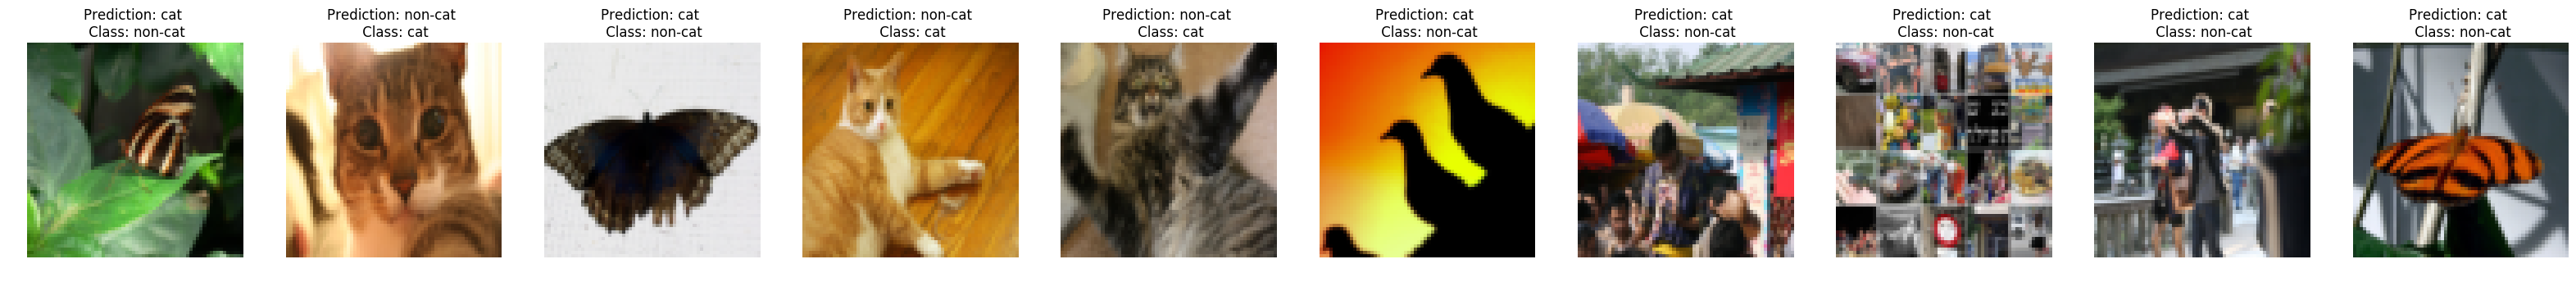
\includegraphics[width=\textwidth]{course1/mislabeled_images} 
  \caption{mislabeled images}
\end{figure}

{\textbf {A few type of images the model tends to do poorly on include}}:
\begin{itemize}
\item Cat body in an unusual position
\item Cat appears against a background of a similar color
\item Unusual cat color and species
\item Camera Angle
\item Brightness of the picture
\item Scale variation (cat is very large or small in image)
\end{itemize}



\subsubsection{Test with your own image (optional/ungraded exercise)}

Congratulations on finishing this assignment. You can use your own image and see the output of your model. To do that:
\begin{itemize}
\item[1.] Click on ``File'' in the upper bar of this notebook, then click ``Open'' to go on your Coursera Hub.
\item[2.] Add your image to this Jupyter Notebook's directory, in the ``images'' folder
\item[3.] Change your image's name in the following code
\item[4.] Run the code and check if the algorithm is right (1 = cat, 0 = non-cat)!
\end{itemize}

\begin{minted}{python}
## START CODE HERE ##
my_image = "test_cat3.jpg" # change this to the name of your image file 
my_label_y = [1] # the true class of your image (1 -> cat, 0 -> non-cat)
## END CODE HERE ##

fname = "images/" + my_image
image = np.array(ndimage.imread(fname, flatten=False))
my_image = scipy.misc.imresize(image, size=(num_px,num_px)).reshape((num_px*num_px*3,1))
my_predicted_image = predict(my_image, my_label_y, parameters)

plt.imshow(image)
print ("y = " + str(np.squeeze(my_predicted_image)) + ", your L-layer model predicts a \"" + classes[int(np.squeeze(my_predicted_image)),].decode("utf-8") +  "\" picture.")


#output:
Accuracy: 1.0
y = 1.0, your L-layer model predicts a "ca" picture.
\end{minted}

\begin{figure}[H]
  \centering
  
\includegraphics[width=0.6\textwidth]{course1/test_cat3} 
\end{figure}

\clearpage
\subsubsection{Code of Deep Neural Network for Image Classification: Application}
\begin{minted}{python}
#matplotlib inline
plt.rcParams['figure.figsize'] = (5.0, 4.0) # set default size of plots
plt.rcParams['image.interpolation'] = 'nearest'
plt.rcParams['image.cmap'] = 'gray'

np.random.seed(1)

#Load the data 
train_x_orig, train_y, test_x_orig, test_y, classes = load_data()

#=====================================================
# #show an image in the dataset. Example of a picture
# index = 12
# plt.imshow(train_x_orig[index])
# print ("y = " + str(train_y[0,index]) + ". It's a " + classes[train_y[0,index]].decode("utf-8") +  " picture.")
#=====================================================

# Explore your dataset 
m_train = train_x_orig.shape[0]
m_test =  test_x_orig.shape[0]
num_px = train_x_orig.shape[1]

# Reshape the training and test examples 
train_x_flatten = train_x_orig.reshape(train_x_orig.shape[0], -1).T   # The "-1" makes reshape flatten the remaining dimensions
test_x_flatten = test_x_orig.reshape(test_x_orig.shape[0], -1).T

# Standardize data to have feature values between 0 and 1.
train_x = train_x_flatten/255.
test_x = test_x_flatten/255.


### CONSTANTS DEFINING THE MODEL ####
n_x = 12288     # num_px * num_px * 3
n_h = 7
n_y = 1
layers_dims = (n_x, n_h, n_y)


# GRADED FUNCTION: two_layer_model

def two_layer_model(X, Y, layers_dims, learning_rate = 0.0075, num_iterations = 3000, print_cost=False):
    """
    Implements a two-layer neural network: LINEAR->RELU->LINEAR->SIGMOID.
    
    Arguments:
    X -- input data, of shape (n_x, number of examples)
    Y -- true "label" vector (containing 0 if cat, 1 if non-cat), of shape (1, number of examples)
    layers_dims -- dimensions of the layers (n_x, n_h, n_y)
    num_iterations -- number of iterations of the optimization loop
    learning_rate -- learning rate of the gradient descent update rule
    print_cost -- If set to True, this will print the cost every 100 iterations 
    
    Returns:
    parameters -- a dictionary containing W1, W2, b1, and b2
    """
    
    np.random.seed(1)
    grads = {}
    costs = []                              # to keep track of the cost
    m = X.shape[1]                           # number of examples
    (n_x, n_h, n_y) = layers_dims
    
    # Initialize parameters dictionary, by calling one of the functions you'd previously implemented
    parameters =initialize_parameters(n_x, n_h, n_y)
    
    # Get W1, b1, W2 and b2 from the dictionary parameters.
    W1 = parameters["W1"]
    b1 = parameters["b1"]
    W2 = parameters["W2"]
    b2 = parameters["b2"]
    
    # Loop (gradient descent)
    for i in range(0, num_iterations):
        # Forward propagation: LINEAR -> RELU -> LINEAR -> SIGMOID. Inputs: "X, W1, b1". Output: "A1, cache1, A2, cache2".
        A1, cache1 = linear_activation_forward(X, W1, b1, "relu")
        A2, cache2 = linear_activation_forward(A1, W2, b2, "sigmoid")
        
        # Compute cost
        cost =  compute_cost(A2, Y)
        
        # Initializing backward propagation
        dA2 = - (np.divide(Y, A2) - np.divide(1 - Y, 1 - A2))
        
        # Backward propagation. Inputs: "dA2, cache2, cache1". Outputs: "dA1, dW2, db2; also dA0 (not used), dW1, db1".
        dA1, dW2, db2 = linear_activation_backward(dA2, cache2, "sigmoid")
        dA0, dW1, db1 = linear_activation_backward(dA1, cache1, "relu")
        
        # Set grads['dWl'] to dW1, grads['db1'] to db1, grads['dW2'] to dW2, grads['db2'] to db2
        grads['dW1'] = dW1
        grads['db1'] = db1
        grads['dW2'] = dW2
        grads['db2'] = db2
        
        # Update parameters.
        parameters = update_parameters(parameters, grads, learning_rate)

        # Retrieve W1, b1, W2, b2 from parameters
        W1 = parameters["W1"]
        b1 = parameters["b1"]
        W2 = parameters["W2"]
        b2 = parameters["b2"]
        
        # Print the cost every 100 training example
        if print_cost and i % 100 == 0:
            print("Cost after iteration {}: {}".format(i, np.squeeze(cost)))
        if print_cost and i % 100 == 0:
            costs.append(cost)
       
    # plot the cost
    plt.plot(np.squeeze(costs))
    plt.ylabel('cost')
    plt.xlabel('iterations (per tens)')
    plt.title("Learning rate =" + str(learning_rate))
    plt.show()
    
    return parameters



# GRADED FUNCTION: L_layer_model
def L_layer_model(X, Y, layers_dims, learning_rate = 0.0075, num_iterations = 3000, print_cost=False):#lr was 0.009
    """
    Implements a L-layer neural network: [LINEAR->RELU]*(L-1)->LINEAR->SIGMOID.
    
    Arguments:
    X -- data, numpy array of shape (number of examples, num_px * num_px * 3)
    Y -- true "label" vector (containing 0 if cat, 1 if non-cat), of shape (1, number of examples)
    layers_dims -- list containing the input size and each layer size, of length (number of layers + 1).
    learning_rate -- learning rate of the gradient descent update rule
    num_iterations -- number of iterations of the optimization loop
    print_cost -- if True, it prints the cost every 100 steps
    
    Returns:
    parameters -- parameters learnt by the model. They can then be used to predict.
    """

    np.random.seed(1)
    costs = []                         # keep track of cost
    
    # Parameters initialization.
    parameters = initialize_parameters_deep(layers_dims)
    
    # Loop (gradient descent)
    for i in range(0, num_iterations):

        # Forward propagation: [LINEAR -> RELU]*(L-1) -> LINEAR -> SIGMOID.
        AL, caches =  L_model_forward(X, parameters)
        
        # Compute cost.
        cost =  compute_cost(AL, Y)
    
        # Backward propagation.
        grads =  L_model_backward(AL, Y, caches)
 
        # Update parameters.
        parameters =  update_parameters(parameters, grads, learning_rate)
                
        # Print the cost every 100 training example
        if print_cost and i % 100 == 0:
            print ("Cost after iteration %i: %f" %(i, cost))
        if print_cost and i % 100 == 0:
            costs.append(cost)
            
    # plot the cost
    plt.plot(np.squeeze(costs))
    plt.ylabel('cost')
    plt.xlabel('iterations (per tens)')
    plt.title("Learning rate =" + str(learning_rate))
    plt.show()
    
    return parameters

### CONSTANTS ###
layers_dims = [12288, 20, 7, 5, 1] #  5-layer model

# two_layer_model
parameters_two_layer_model = two_layer_model(train_x, train_y, layers_dims = (n_x, n_h, n_y), num_iterations = 2500, print_cost=True)
predictions_train = predict(train_x, train_y, parameters_two_layer_model)
predictions_test = predict(test_x, test_y, parameters_two_layer_model)


# L_layer_model
parameters_L_layer_model = L_layer_model(train_x, train_y, layers_dims, num_iterations = 2500, print_cost = True)
pred_train = predict(train_x, train_y, parameters_L_layer_model)
pred_test = predict(test_x, test_y, parameters_L_layer_model)
\end{minted}
\clearpage

% Course2 Improving Deep Neural Networks: Hyperparameter tuning, Regularization and Optimization
\section{Improving Deep Neural Networks: Hyperparameter tuning, Regularization and Optimization}

\subsection{Practical aspects of Deep Learning}

Welcome to the first assignment of the hyper parameters tuning specialization. It is very important that you regularize your model properly because it could dramatically improve your results.
\begin{figure}[h]
\begin{center}
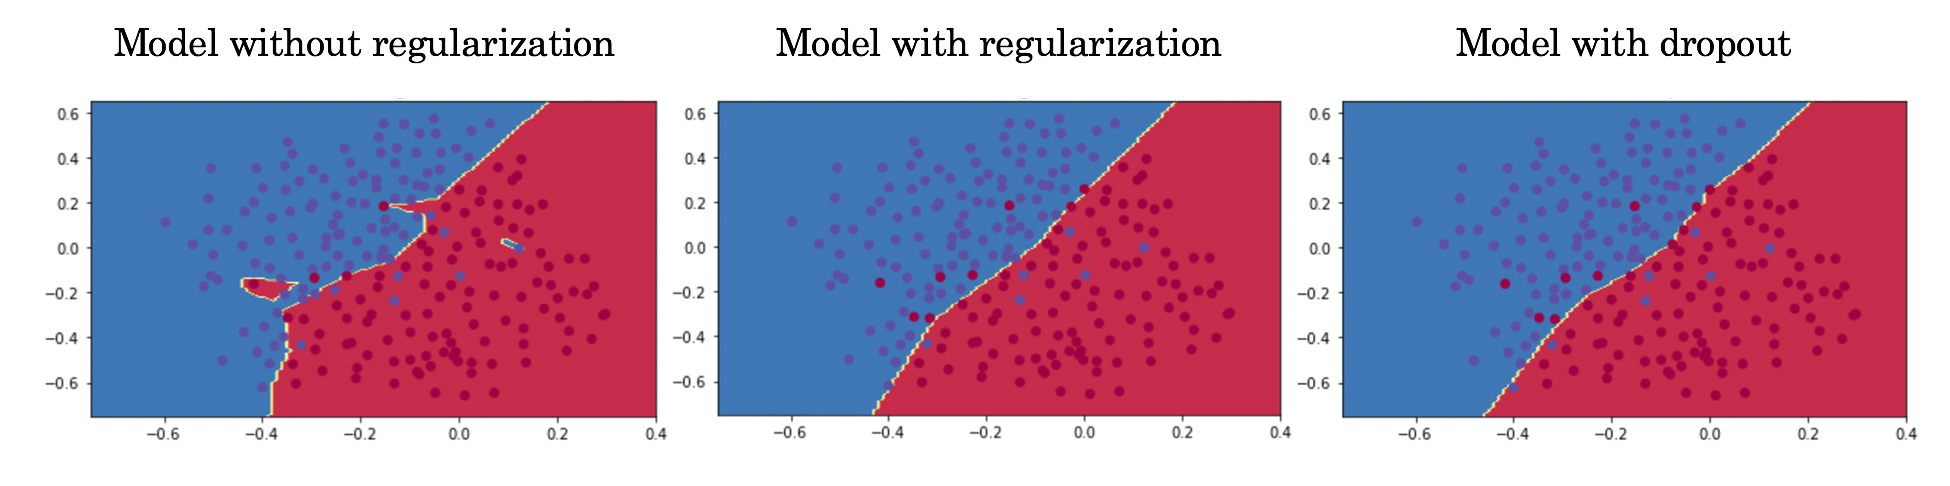
\includegraphics[width=\textwidth]{course2/Initialization}
\end{center}
\end{figure}

By completing this assignment you will:
\begin{itemize}
\item Understand that different regularization methods that could help your model.
\item Implement dropout and see it work on data.
\item Recognize that a model without regularization gives you a better accuracy on the training set but nor necessarily on the test set.
\item Understand that you could use both dropout and regularization on your model.
\end{itemize}

This assignment prepares you well for the upcoming assignment. Take your time to complete it and make sure you get the expected outputs when working through the different exercises. In some code blocks, you will find a "\#GRADED FUNCTION: functionName" comment. Please do not modify it. After you are done, submit your work and check your results. You need to score 80\% to pass. Good luck :) !


\subsubsection{Initialization}

Welcome to the first assignment of ``Improving Deep Neural Networks".

Training your neural network requires specifying an initial value of the weights. A well chosen initialization method will help learning.

If you completed the previous course of this specialization, you probably followed our instructions for weight initialization, and it has worked out so far. But how do you choose the initialization for a new neural network? In this notebook, you will see how different initializations lead to different results.

A well chosen initialization can:
\begin{itemize}
\item Speed up the convergence of gradient descent
\item Increase the odds of gradient descent converging to a lower training (and generalization) error
\end{itemize}


\subsubsubsection{Packages}
To get started, run the following code to load the packages and the planar dataset you will try to classify.
\begin{minted}{python}
import numpy as np
import matplotlib.pyplot as plt
import sklearn
import sklearn.datasets
from init_utils import sigmoid, relu, compute_loss, forward_propagation, backward_propagation
from init_utils import update_parameters, predict, load_dataset, plot_decision_boundary, predict_dec

# matplotlib inline
plt.rcParams['figure.figsize'] = (7.0, 4.0) # set default size of plots
plt.rcParams['image.interpolation'] = 'nearest'
plt.rcParams['image.cmap'] = 'gray'

# load image dataset: blue/red dots in circles
train_X, train_Y, test_X, test_Y = load_dataset()
\end{minted}
\begin{figure}[h]
\begin{center}
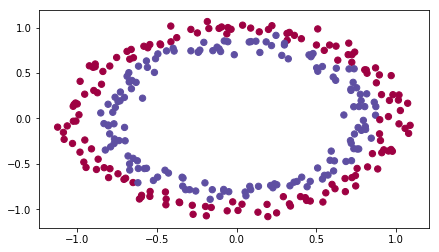
\includegraphics[width=0.7\textwidth]{course2/blue_red_dots}
\end{center}
\end{figure}

You would like a classifier to separate the blue dots from the red dots.


\subsubsubsection{Neural Network model}

You will use a 3-layer neural network (already implemented for you). Here are the initialization methods you will experiment with:
\begin{itemize}
\item \emph{Zeros initialization} -- setting initialization = ``zeros" in the input argument.
\item \emph{Random initialization} -- setting initialization = ``random" in the input argument. This initializes the weights to large random values.
\item \emph{He initialization} -- setting initialization = ``he" in the input argument. This initializes the weights to random values scaled according to a paper by \href{https://arxiv.org/abs/1512.03385}{He et al., 2015}.
\end{itemize}
{\textbf {Instructions}}: Please quickly read over the code below, and run it. In the next part you will implement the three initialization methods that this model() calls.

\begin{minted}{python}
def model(X, Y, learning_rate = 0.01, num_iterations = 15000, print_cost = True, initialization = "he"):
    """
    Implements a three-layer neural network: LINEAR->RELU->LINEAR->RELU->LINEAR->SIGMOID.
    
    Arguments:
    X -- input data, of shape (2, number of examples)
    Y -- true "label" vector (containing 0 for red dots; 1 for blue dots), of shape (1, number of examples)
    learning_rate -- learning rate for gradient descent 
    num_iterations -- number of iterations to run gradient descent
    print_cost -- if True, print the cost every 1000 iterations
    initialization -- flag to choose which initialization to use ("zeros","random" or "he")
    
    Returns:
    parameters -- parameters learnt by the model
    """
        
    grads = {}
    costs = [] # to keep track of the loss
    m = X.shape[1] # number of examples
    layers_dims = [X.shape[0], 10, 5, 1]
    
    # Initialize parameters dictionary.
    if initialization == "zeros":
        parameters = initialize_parameters_zeros(layers_dims)
    elif initialization == "random":
        parameters = initialize_parameters_random(layers_dims)
    elif initialization == "he":
        parameters = initialize_parameters_he(layers_dims)

    # Loop (gradient descent)

    for i in range(0, num_iterations):

        # Forward propagation: LINEAR -> RELU -> LINEAR -> RELU -> LINEAR -> SIGMOID.
        a3, cache = forward_propagation(X, parameters)
        
        # Loss
        cost = compute_loss(a3, Y)

        # Backward propagation.
        grads = backward_propagation(X, Y, cache)
        
        # Update parameters.
        parameters = update_parameters(parameters, grads, learning_rate)
        
        # Print the loss every 1000 iterations
        if print_cost and i % 1000 == 0:
            print("Cost after iteration {}: {}".format(i, cost))
            costs.append(cost)
            
    # plot the loss
    plt.plot(costs)
    plt.ylabel('cost')
    plt.xlabel('iterations (per hundreds)')
    plt.title("Learning rate =" + str(learning_rate))
    plt.show()
    
    return parameters
\end{minted}


\subsubsubsection{Zero initialization}

There are two types of parameters to initialize in a neural network:
\begin{itemize}
\item the weight matrices $(W^{[1]}, W^{[2]}, W^{[3]}, ..., W^{[L-1]}, W^{[L]})$
\item the bias vectors $(b^{[1]}, b^{[2]}, b^{[3]}, ..., b^{[L-1]}, b^{[L]})$
\end{itemize}

{\textbf {Exercise}}: Implement the following function to initialize all parameters to zeros. You'll see later that this does not work well since it fails to "break symmetry", but lets try it anyway and see what happens. Use np.zeros((..,..)) with the correct shapes.
\begin{minted}{python}
# GRADED FUNCTION: initialize_parameters_zeros 
def initialize_parameters_zeros(layers_dims):
    """
    Arguments:
    layer_dims -- python array (list) containing the size of each layer.
    
    Returns:
    parameters -- python dictionary containing your parameters "W1", "b1", ..., "WL", "bL":
            W1 -- weight matrix of shape (layers_dims[1], layers_dims[0])
            b1 -- bias vector of shape (layers_dims[1], 1)
                  ...
            WL -- weight matrix of shape (layers_dims[L], layers_dims[L-1])
            bL -- bias vector of shape (layers_dims[L], 1)
    """
    
    parameters = {}
    L = len(layers_dims)            # number of layers in the network
    
    for l in range(1, L):
        ### START CODE HERE ### (≈ 2 lines of code)
        parameters['W' + str(l)] = np.zeros((layers_dims[l],layers_dims[l-1])) 
        parameters['b' + str(l)] = np.zeros((layers_dims[l],1)) 
        ### END CODE HERE ###
    return parameters
\end{minted}

\begin{minted}{python}
parameters = initialize_parameters_zeros([3,2,1])
print("W1 = " + str(parameters["W1"]))
print("b1 = " + str(parameters["b1"]))
print("W2 = " + str(parameters["W2"]))
print("b2 = " + str(parameters["b2"]))

#output
W1 = [[ 0.  0.  0.]
 [ 0.  0.  0.]]
b1 = [[ 0.]
 [ 0.]]
W2 = [[ 0.  0.]]
b2 = [[ 0.]]

\end{minted}

Run the following code to train your model on 15,000 iterations using zeros initialization.
\begin{minted}{python}
parameters = model(train_X, train_Y, initialization = "zeros")
print ("On the train set:")
predictions_train = predict(train_X, train_Y, parameters)
print ("On the test set:")
predictions_test = predict(test_X, test_Y, parameters)
\end{minted}
\begin{minted}{python}
#output
Cost after iteration 0: 0.6931471805599453
Cost after iteration 1000: 0.6931471805599453
Cost after iteration 2000: 0.6931471805599453
Cost after iteration 3000: 0.6931471805599453
Cost after iteration 4000: 0.6931471805599453
Cost after iteration 5000: 0.6931471805599453
Cost after iteration 6000: 0.6931471805599453
Cost after iteration 7000: 0.6931471805599453
Cost after iteration 8000: 0.6931471805599453
Cost after iteration 9000: 0.6931471805599453
Cost after iteration 10000: 0.6931471805599455
Cost after iteration 11000: 0.6931471805599453
Cost after iteration 12000: 0.6931471805599453
Cost after iteration 13000: 0.6931471805599453
Cost after iteration 14000: 0.6931471805599453

On the train set:
Accuracy: 0.5
On the test set:
Accuracy: 0.5
\end{minted}

\begin{figure}[h]
\begin{center}
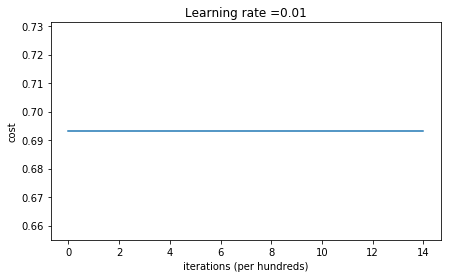
\includegraphics[width=0.7\textwidth]{course2/initialize_parameters_zeros_cost}
\end{center}
\end{figure}

The performance is really bad, and the cost does not really decrease, and the algorithm performs no better than random guessing. Why? Lets look at the details of the predictions and the decision boundary:
\begin{minted}{python}
print ("predictions_train = " + str(predictions_train))
print ("predictions_test = " + str(predictions_test))

#output
predictions_train = [[0 0 0 0 0 0 0 0 0 0 0 0 0 0 0 0 0 0 0 0 0 0 0 0 0 0 0 0 0 0 0 0 0 0 0 0 0
  0 0 0 0 0 0 0 0 0 0 0 0 0 0 0 0 0 0 0 0 0 0 0 0 0 0 0 0 0 0 0 0 0 0 0 0 0
  0 0 0 0 0 0 0 0 0 0 0 0 0 0 0 0 0 0 0 0 0 0 0 0 0 0 0 0 0 0 0 0 0 0 0 0 0
  0 0 0 0 0 0 0 0 0 0 0 0 0 0 0 0 0 0 0 0 0 0 0 0 0 0 0 0 0 0 0 0 0 0 0 0 0
  0 0 0 0 0 0 0 0 0 0 0 0 0 0 0 0 0 0 0 0 0 0 0 0 0 0 0 0 0 0 0 0 0 0 0 0 0
  0 0 0 0 0 0 0 0 0 0 0 0 0 0 0 0 0 0 0 0 0 0 0 0 0 0 0 0 0 0 0 0 0 0 0 0 0
  0 0 0 0 0 0 0 0 0 0 0 0 0 0 0 0 0 0 0 0 0 0 0 0 0 0 0 0 0 0 0 0 0 0 0 0 0
  0 0 0 0 0 0 0 0 0 0 0 0 0 0 0 0 0 0 0 0 0 0 0 0 0 0 0 0 0 0 0 0 0 0 0 0 0
  0 0 0 0]]
predictions_test = [[0 0 0 0 0 0 0 0 0 0 0 0 0 0 0 0 0 0 0 0 0 0 0 0 0 0 0 0 0 0 0 0 0 0 0 0 0
  0 0 0 0 0 0 0 0 0 0 0 0 0 0 0 0 0 0 0 0 0 0 0 0 0 0 0 0 0 0 0 0 0 0 0 0 0
  0 0 0 0 0 0 0 0 0 0 0 0 0 0 0 0 0 0 0 0 0 0 0 0 0 0]]
\end{minted}
\begin{minted}{python}
plt.title("Model with Zeros initialization")
axes = plt.gca()
axes.set_xlim([-1.5,1.5])
axes.set_ylim([-1.5,1.5])
plot_decision_boundary(lambda x: predict_dec(parameters, x.T), train_X, train_Y)
\end{minted}
\begin{figure}[h]
\begin{center}
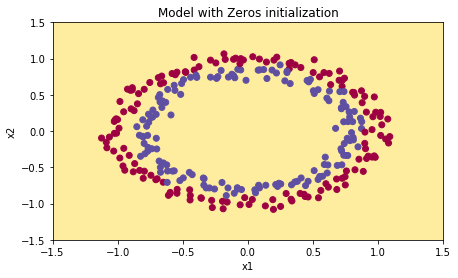
\includegraphics[width=0.7\textwidth]{course2/Model_with_Zeros_initialization}
\caption{Model with Zeros initialization}
\end{center}
\end{figure}

The model is predicting 0 for every example.

In general, initializing all the weights to zero results in the network failing to break symmetry. This means that every neuron in each layer will learn the same thing, and you might as well be training a neural network with  $n^{[l]}=1$  for every layer, and the network is no more powerful than a linear classifier such as logistic regression.

{\color{red} \textbf {
What you should remember:
\begin{itemize}
\item The weights  $W^{[l]}$  should be initialized randomly to break symmetry.
\item It is however okay to initialize the biases  $b^{[l]}$  to zeros. Symmetry is still broken so long as  $W^{[l]}$ is initialized randomly.
\end{itemize}
}}

\subsubsubsection{Random initialization}

To break symmetry, lets intialize the weights randomly. Following random initialization, each neuron can then proceed to learn a different function of its inputs. In this exercise, you will see what happens if the weights are intialized randomly, but to very large values.

{\textbf {Exercise}}: Implement the following function to initialize your weights to large random values (scaled by *10) and your biases to zeros. Use np.random.randn(..,..)*10 for weights and np.zeros((.., ..)) for biases. We are using a fixed np.random.seed(..) to make sure your ``random" weights match ours, so don't worry if running several times your code gives you always the same initial values for the parameters.

\begin{minted}{python}
# GRADED FUNCTION: initialize_parameters_random
def initialize_parameters_random(layers_dims):
    """
    Arguments:
    layer_dims -- python array (list) containing the size of each layer.
    
    Returns:
    parameters -- python dictionary containing your parameters "W1", "b1", ..., "WL", "bL":
                    W1 -- weight matrix of shape (layers_dims[1], layers_dims[0])
                    b1 -- bias vector of shape (layers_dims[1], 1)
                    ...
                    WL -- weight matrix of shape (layers_dims[L], layers_dims[L-1])
                    bL -- bias vector of shape (layers_dims[L], 1)
    """
    
    np.random.seed(3)               # This seed makes sure your "random" numbers will be the as ours
    parameters = {}
    L = len(layers_dims)            # integer representing the number of layers
    
    for l in range(1, L):
        ### START CODE HERE ### (≈ 2 lines of code)
        parameters['W' + str(l)] = np.random.randn(layers_dims[L], layers_dims[L-1]) * 10
        parameters['b' + str(l)] = np.zeros((layers_dims[L], 1))
        ### END CODE HERE ###

    return parameters
\end{minted}
\begin{minted}{python}
parameters = initialize_parameters_random([3, 2, 1])
print("W1 = " + str(parameters["W1"]))
print("b1 = " + str(parameters["b1"]))
print("W2 = " + str(parameters["W2"]))
print("b2 = " + str(parameters["b2"]))    

#output
W1 = [[ 17.88628473   4.36509851   0.96497468]
 [-18.63492703  -2.77388203  -3.54758979]]
b1 = [[ 0.]
 [ 0.]]
W2 = [[-0.82741481 -6.27000677]]
b2 = [[ 0.]]
\end{minted}

Run the following code to train your model on 15,000 iterations using random initialization.
\begin{minted}{python}
parameters = model(train_X, train_Y, initialization = "random")
print ("On the train set:")
predictions_train = predict(train_X, train_Y, parameters)
print ("On the test set:")
predictions_test = predict(test_X, test_Y, parameters)

#output
Cost after iteration 0: inf
Cost after iteration 1000: 0.6237287551108738
Cost after iteration 2000: 0.5981106708339466
......
Cost after iteration 14000: 0.38278397192120406

#Accuracy
On the train set:
Accuracy: 0.83
On the test set:
Accuracy: 0.86
\end{minted}
\vspace{-0.5cm}
\begin{figure}[h]
\begin{center}
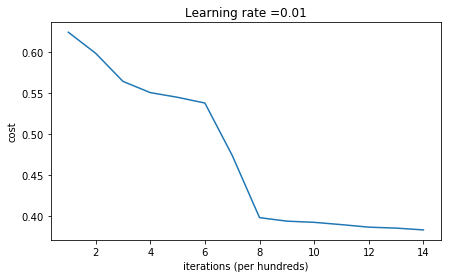
\includegraphics[width=0.7\textwidth]{course2/initialize_parameters_random_cost}
\end{center}
\end{figure}


If you see ``inf" as the cost after the iteration 0, this is because of numerical roundoff; a more numerically sophisticated implementation would fix this. But this isn't worth worrying about for our purposes.

Anyway, it looks like you have broken symmetry, and this gives better results. than before. The model is no longer outputting all 0s.

\begin{minted}{python}
print (predictions_train)
print (predictions_test)

#output
[[1 0 1 1 0 0 1 1 1 1 1 0 1 0 0 1 0 1 1 0 0 0 1 0 1 1 1 1 1 1 0 1 1 0 0 1 1
  1 1 1 1 1 1 0 1 1 1 1 0 1 0 1 1 1 1 0 0 1 1 1 1 0 1 1 0 1 0 1 1 1 1 0 0 0
  0 0 1 0 1 0 1 1 1 0 0 1 1 1 1 1 1 0 0 1 1 1 0 1 1 0 1 0 1 1 0 1 1 0 1 0 1
  1 0 0 1 0 0 1 1 0 1 1 1 0 1 0 0 1 0 1 1 1 1 1 1 1 0 1 1 0 0 1 1 0 0 0 1 0
  1 0 1 0 1 1 1 0 0 1 1 1 1 0 1 1 0 1 0 1 1 0 1 0 1 1 1 1 0 1 1 1 1 0 1 0 1
  0 1 1 1 1 0 1 1 0 1 1 0 1 1 0 1 0 1 1 1 0 1 1 1 0 1 0 1 0 0 1 0 1 1 0 1 1
  0 1 1 0 1 1 1 0 1 1 1 1 0 1 0 0 1 1 0 1 1 1 0 0 0 1 1 0 1 1 1 1 0 1 1 0 1
  1 1 0 0 1 0 0 0 1 0 0 0 1 1 1 1 0 0 0 0 1 1 1 1 0 0 1 1 1 1 1 1 1 0 0 0 1
  1 1 1 0]]
[[1 1 1 1 0 1 0 1 1 0 1 1 1 0 0 0 0 1 0 1 0 0 1 0 1 0 1 1 1 1 1 0 0 0 0 1 0
  1 1 0 0 1 1 1 1 1 0 1 1 1 0 1 0 1 1 0 1 0 1 0 1 1 1 1 1 1 1 1 1 0 1 0 1 1
  1 1 1 0 1 0 0 1 0 0 0 1 1 0 1 1 0 0 0 1 1 0 1 1 0 0]]
\end{minted}

\begin{figure}[h]
\begin{center}
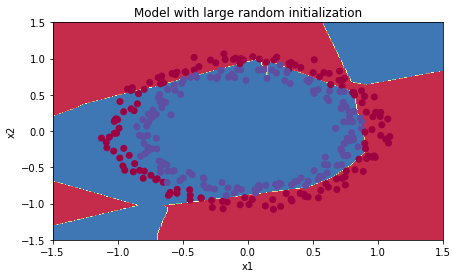
\includegraphics[width=0.6\textwidth]{course2/initialize_parameters_random}
\caption{Model with random initialization}
\end{center}
\end{figure}


\begin{minted}{python}
plt.title("Model with large random initialization")
axes = plt.gca()
axes.set_xlim([-1.5,1.5])
axes.set_ylim([-1.5,1.5])
plot_decision_boundary(lambda x: predict_dec(parameters, x.T), train_X, train_Y)
\end{minted}


{\textbf {Observations}}:
\begin{itemize}
\item The cost starts very high. This is because with large random-valued weights, the last activation (sigmoid) outputs results that are very close to 0 or 1 for some examples, and when it gets that example wrong it incurs a very high loss for that example. Indeed, when  $log(a^{[3]})=log(0)$, the loss goes to infinity.
\item Poor initialization can lead to vanishing/exploding gradients, which also slows down the optimization algorithm.
\item If you train this network longer you will see better results, but initializing with overly large random numbers slows down the optimization.
\end{itemize}

{\color{red} \textbf {In summary:
\begin{itemize}
\item Initializing weights to very large random values does not work well.
\item Hopefully intializing with small random values does better. The important question is: how small should be these random values be? Lets find out in the next part!
\end{itemize}
}}


\subsubsubsection{He initialization}

Finally, try ``He Initialization"; this is named for the first author of He et al., 2015. (If you have heard of ``Xavier initialization", this is similar except Xavier initialization uses a scaling factor for the weights $W^{[l]}$ of \emph{sqrt(1./layers\_dims[l-1])} where He initialization would use \emph{sqrt(2./layers\_dims[l-1])}.)

{\textbf {Exercise}}: Implement the following function to initialize your parameters with He initialization.

{\textbf {Hint}}: This function is similar to the previous \emph{initialize\_parameters\_random(...)}. The only difference is that instead of multiplying \emph{np.random.randn(..,..)} by 10, you will multiply it by $\sqrt{\frac{2}{\text{dimension of the previous layer}}}$, which is what He initialization recommends for layers with a ReLU activation. 

\begin{minted}{python}
# GRADED FUNCTION: initialize_parameters_he
def initialize_parameters_he(layers_dims):
    """
    Arguments:
    layer_dims -- python array (list) containing the size of each layer.
    
    Returns:
    parameters -- python dictionary containing your parameters "W1", "b1", ..., "WL", "bL":
                    W1 -- weight matrix of shape (layers_dims[1], layers_dims[0])
                    b1 -- bias vector of shape (layers_dims[1], 1)
                    ...
                    WL -- weight matrix of shape (layers_dims[L], layers_dims[L-1])
                    bL -- bias vector of shape (layers_dims[L], 1)
    """
    
    np.random.seed(3)
    parameters = {}
    L = len(layers_dims) - 1 # integer representing the number of layers
     
    for l in range(1, L + 1):
        ### START CODE HERE ### (≈ 2 lines of code)
        parameters['W' + str(l)] = np.random.randn(layers_dims[l], layers_dims[l-1]) * np.sqrt(2./layers_dims[l-1])
        parameters['b' + str(l)] = np.zeros((layers_dims[l], 1))
        ### END CODE HERE ###
        
    return parameters
\end{minted}

\begin{minted}{python}
parameters = initialize_parameters_he([2, 4, 1])
print("W1 = " + str(parameters["W1"]))
print("b1 = " + str(parameters["b1"]))
print("W2 = " + str(parameters["W2"]))
print("b2 = " + str(parameters["b2"]))

#output
1 = [[ 1.78862847  0.43650985]
 [ 0.09649747 -1.8634927 ]
 [-0.2773882  -0.35475898]
 [-0.08274148 -0.62700068]]
b1 = [[ 0.]
 [ 0.]
 [ 0.]
 [ 0.]]
W2 = [[-0.03098412 -0.33744411 -0.92904268  0.62552248]]
b2 = [[ 0.]]
\end{minted}

Run the following code to train your model on 15,000 iterations using He initialization.
\vspace{-0.5cm}
\begin{minted}{python}
parameters = model(train_X, train_Y, initialization = "he")
print ("On the train set:")
predictions_train = predict(train_X, train_Y, parameters)
print ("On the test set:")
predictions_test = predict(test_X, test_Y, parameters)

#output
Cost after iteration 0: 0.8830537463419761
Cost after iteration 1000: 0.6879825919728063
......
Cost after iteration 13000: 0.0845705595402428
Cost after iteration 14000: 0.07357895962677366

#Accuracy
On the train set:
Accuracy: 0.993333333333
On the test set:
Accuracy: 0.96

\end{minted}

\vspace{-0.3cm}
\begin{figure}[h]
\begin{center}
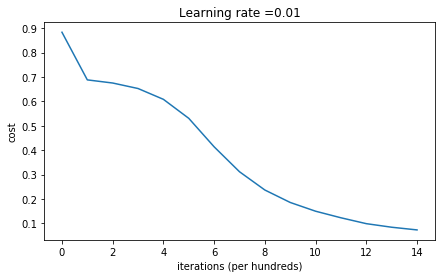
\includegraphics[width=0.6\textwidth]{course2/initialize_parameters_HE_cost}
\end{center}
\end{figure}

\vspace{-1cm}
\begin{minted}{python}
plt.title("Model with He initialization")
axes = plt.gca()
axes.set_xlim([-1.5,1.5])
axes.set_ylim([-1.5,1.5])
plot_decision_boundary(lambda x: predict_dec(parameters, x.T), train_X, train_Y)
\end{minted}

\begin{figure}[h]
\begin{center}
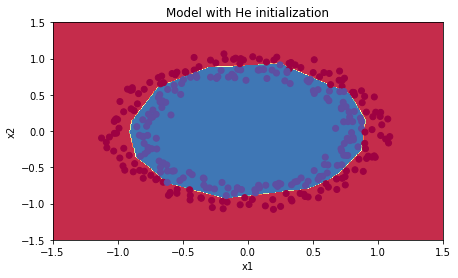
\includegraphics[width=0.6\textwidth]{course2/initialize_parameters_HE}
\caption{Model with He initialization}
\end{center}
\end{figure}


{\textbf {Observations}}:

The model with He initialization separates the blue and the red dots very well in a small number of iterations.


\subsubsubsection{Conclusions}

You have seen three different types of initializations. For the same number of iterations and same hyperparameters the comparison is:
\begin{table}[H]
\centering
\begin{tabular}{ccc}  
\toprule
Model&	Train accuracy	&Problem/Comment\\
\midrule
3-layer NN with zeros initialization	& 50\%	& fails to break symmetry\\
3-layer NN with large random initialization	& 83\%	& too large weights\\
3-layer NN with He initialization	&99\%	& recommended method\\
\bottomrule
\end{tabular}
\end{table}

{\color{red} \textbf{
What you should remember from this assignment:
\begin{itemize}
\item Different initializations lead to different results
\item Random initialization is used to break symmetry and make sure different hidden units can learn different things
\item Don't intialize to values that are too large
\item He initialization works well for networks with ReLU activations.
\end{itemize}
}}



\clearpage
\subsubsubsection{Code of initialization}
\begin{minted}{python}
import numpy as np
import matplotlib.pyplot as plt
import sklearn
import sklearn.datasets
from init_utils import sigmoid, relu, compute_loss, forward_propagation, backward_propagation
from init_utils import update_parameters, predict, load_dataset, plot_decision_boundary, predict_dec

#===========================================
# # matplotlib inline
# plt.rcParams['figure.figsize'] = (7.0, 4.0) # set default size of plots
# plt.rcParams['image.interpolation'] = 'nearest'
# plt.rcParams['image.cmap'] = 'gray'
#===========================================

# load image dataset: blue/red dots in circles
#train_X, train_Y, test_X, test_Y = load_dataset()

def model(X, Y, learning_rate = 0.01, num_iterations = 15000, print_cost = True, initialization = "he"):
    """
    Implements a three-layer neural network: LINEAR->RELU->LINEAR->RELU->LINEAR->SIGMOID.
    
    Arguments:
    X -- input data, of shape (2, number of examples)
    Y -- true "label" vector (containing 0 for red dots; 1 for blue dots), of shape (1, number of examples)
    learning_rate -- learning rate for gradient descent 
    num_iterations -- number of iterations to run gradient descent
    print_cost -- if True, print the cost every 1000 iterations
    initialization -- flag to choose which initialization to use ("zeros","random" or "he")
    
    Returns:
    parameters -- parameters learnt by the model
    """
        
    grads = {}
    costs = [] # to keep track of the loss
    m = X.shape[1] # number of examples
    layers_dims = [X.shape[0], 10, 5, 1]
    
    # Initialize parameters dictionary.
    if initialization == "zeros":
        parameters = initialize_parameters_zeros(layers_dims)
    elif initialization == "random":
        parameters = initialize_parameters_random(layers_dims)
    elif initialization == "he":
        parameters = initialize_parameters_he(layers_dims)

    # Loop (gradient descent)
    for i in range(0, num_iterations):

        # Forward propagation: LINEAR -> RELU -> LINEAR -> RELU -> LINEAR -> SIGMOID.
        a3, cache = forward_propagation(X, parameters)
        
        # Loss
        cost = compute_loss(a3, Y)

        # Backward propagation.
        grads = backward_propagation(X, Y, cache)
        
        # Update parameters.
        parameters = update_parameters(parameters, grads, learning_rate)
        
        # Print the loss every 1000 iterations
        if print_cost and i % 1000 == 0:
            print("Cost after iteration {}: {}".format(i, cost))
            costs.append(cost)
            
    # plot the loss
    plt.plot(costs)
    plt.ylabel('cost')
    plt.xlabel('iterations (per hundreds)')
    plt.title("Learning rate =" + str(learning_rate))
    plt.show()
    
    return parameters


# GRADED FUNCTION: initialize_parameters_zeros 
def initialize_parameters_zeros(layers_dims):
    """
    Arguments:
    layer_dims -- python array (list) containing the size of each layer.
    
    Returns:
    parameters -- python dictionary containing your parameters "W1", "b1", ..., "WL", "bL":
                    W1 -- weight matrix of shape (layers_dims[1], layers_dims[0])
                    b1 -- bias vector of shape (layers_dims[1], 1)
                    ...
                    WL -- weight matrix of shape (layers_dims[L], layers_dims[L-1])
                    bL -- bias vector of shape (layers_dims[L], 1)
    """
    
    parameters = {}
    L = len(layers_dims)            # number of layers in the network
    
    for l in range(1, L):
        parameters['W' + str(l)] = np.zeros((layers_dims[l],layers_dims[l-1])) 
        parameters['b' + str(l)] = np.zeros((layers_dims[l],1)) 
    return parameters


# GRADED FUNCTION: initialize_parameters_random
def initialize_parameters_random(layers_dims):
    """
    Arguments:
    layer_dims -- python array (list) containing the size of each layer.
    
    Returns:
    parameters -- python dictionary containing your parameters "W1", "b1", ..., "WL", "bL":
                    W1 -- weight matrix of shape (layers_dims[1], layers_dims[0])
                    b1 -- bias vector of shape (layers_dims[1], 1)
                    ...
                    WL -- weight matrix of shape (layers_dims[L], layers_dims[L-1])
                    bL -- bias vector of shape (layers_dims[L], 1)
    """
    
    np.random.seed(3)  # This seed makes sure your "random" numbers will be the as ours
    parameters = {}
    L = len(layers_dims)  # integer representing the number of layers
    
    for l in range(1, L):
        parameters['W' + str(l)] = np.random.randn(layers_dims[l], layers_dims[l-1]) * 10
        parameters['b' + str(l)] = np.zeros((layers_dims[l], 1))

    return parameters


# GRADED FUNCTION: initialize_parameters_he
def initialize_parameters_he(layers_dims):
    """
    Arguments:
    layer_dims -- python array (list) containing the size of each layer.
    
    Returns:
    parameters -- python dictionary containing your parameters "W1", "b1", ..., "WL", "bL":
                    W1 -- weight matrix of shape (layers_dims[1], layers_dims[0])
                    b1 -- bias vector of shape (layers_dims[1], 1)
                    ...
                    WL -- weight matrix of shape (layers_dims[L], layers_dims[L-1])
                    bL -- bias vector of shape (layers_dims[L], 1)
    """
    
    np.random.seed(3)
    parameters = {}
    L = len(layers_dims) - 1 # integer representing the number of layers
     
    for l in range(1, L + 1):
        parameters['W' + str(l)] = np.random.randn(layers_dims[l], layers_dims[l-1]) * np.sqrt(2./layers_dims[l-1])
        parameters['b' + str(l)] = np.zeros((layers_dims[l], 1))
        
    return parameters


#parameters = initialize_parameters_zeros([3,2,1])
#parameters = initialize_parameters_random([3, 2, 1])
parameters = initialize_parameters_he([2, 4, 1])
print("W1 = " + str(parameters["W1"]))
print("b1 = " + str(parameters["b1"]))
print("W2 = " + str(parameters["W2"]))
print("b2 = " + str(parameters["b2"]))

parameters = model(train_X, train_Y, initialization = "he")
print ("On the train set:")
predictions_train = predict(train_X, train_Y, parameters)
print ("On the test set:")
predictions_test = predict(test_X, test_Y, parameters)

plt.title("Model with He initialization")
axes = plt.gca()
axes.set_xlim([-1.5,1.5])
axes.set_ylim([-1.5,1.5])
plot_decision_boundary(lambda x: predict_dec(parameters, x.T), train_X, train_Y)
\end{minted}
\clearpage
\subsubsection{Regularization}

Welcome to the second assignment of this week. Deep Learning models have so much flexibility and capacity that overfitting can be a serious problem, if the training dataset is not big enough. Sure it does well on the training set, but the learned network doesn't generalize to new examples that it has never seen!

{\textbf{You will learn to}}: Use regularization in your deep learning models.


Let's first import the packages you are going to use.
\begin{minted}{python}
# import packages
import numpy as np
import matplotlib.pyplot as plt
from reg_utils import sigmoid, relu, plot_decision_boundary, initialize_parameters, load_2D_dataset, predict_dec
from reg_utils import compute_cost, predict, forward_propagation, backward_propagation, update_parameters
import sklearn
import sklearn.datasets
import scipy.io
from testCases import *

#matplotlib inline
plt.rcParams['figure.figsize'] = (7.0, 4.0) # set default size of plots
plt.rcParams['image.interpolation'] = 'nearest'
plt.rcParams['image.cmap'] = 'gray'
\end{minted}

{\textbf {Problem Statement}}: You have just been hired as an AI expert by the French Football Corporation. They would like you to recommend positions where France's goal keeper should kick the ball so that the French team's players can then hit it with their head.

\begin{figure}[h]
\begin{center}
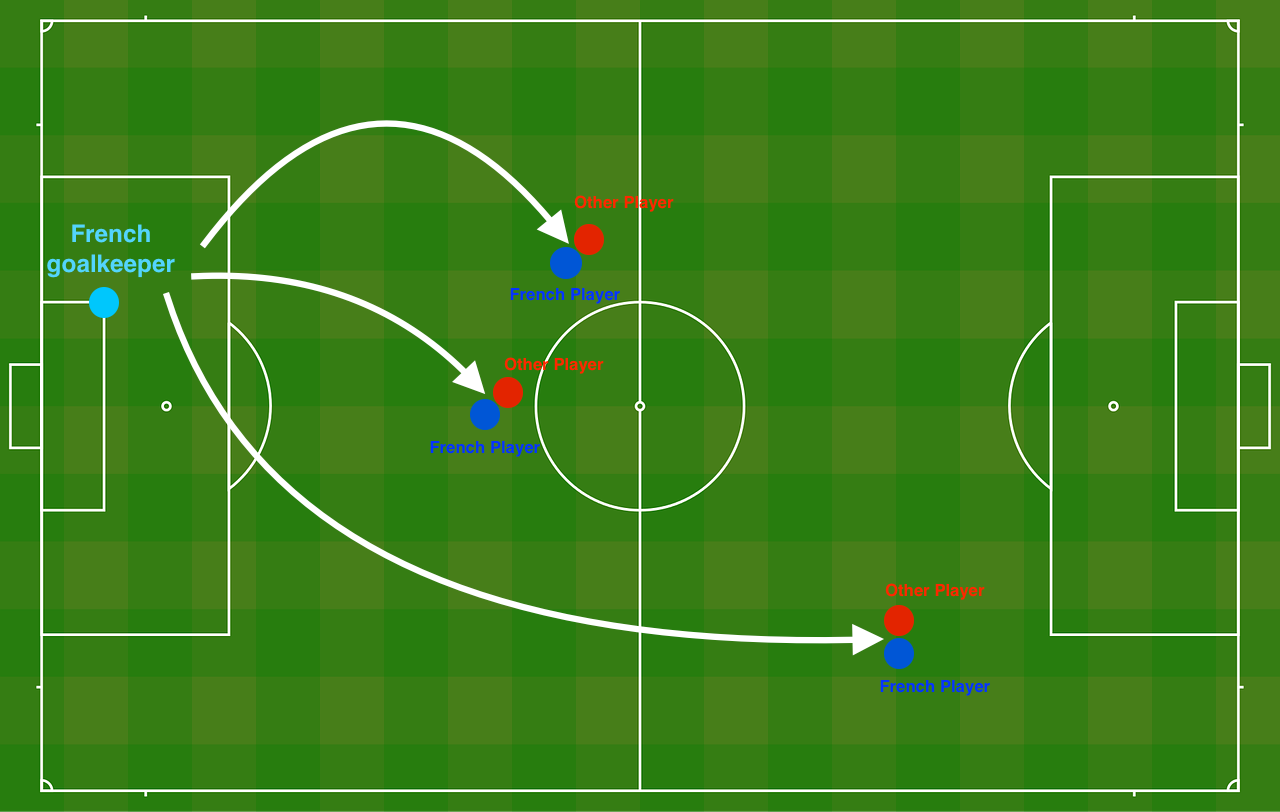
\includegraphics[width=0.5\textwidth]{course2/Football_field}
\caption{The goal keeper kicks the ball in the air, the players of each team are fighting to hit the ball with their head}
\end{center}
\end{figure}

They give you the following 2D dataset from France's past 10 games.
\begin{minted}{python}
train_X, train_Y, test_X, test_Y = load_2D_dataset()
\end{minted}
\vspace{-0.4cm}
\begin{figure}[h]
\begin{center}
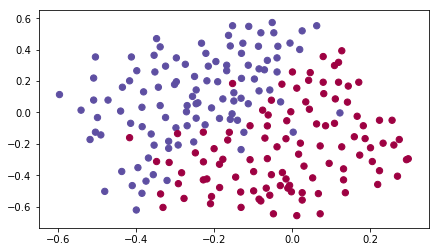
\includegraphics[width=0.7\textwidth]{course2/load_2D_dataset}
\caption{ 2D dataset from France's past 10 games}
\end{center}
\end{figure}

Each dot corresponds to a position on the football field where a football player has hit the ball with his/her head after the French goal keeper has shot the ball from the left side of the football field.
\begin{itemize}
\item If the dot is blue, it means the French player managed to hit the ball with his/her head
\item If the dot is red, it means the other team's player hit the ball with their head
\end{itemize}

{\textbf {Your goal}}: Use a deep learning model to find the positions on the field where the goalkeeper should kick the ball.

{\textbf {Analysis of the dataset}}: This dataset is a little noisy, but it looks like a diagonal line separating the upper left half (blue) from the lower right half (red) would work well.

You will first try a non-regularized model. Then you'll learn how to regularize it and decide which model you will choose to solve the French Football Corporation's problem.


\subsubsubsection{Non-regularized model}

You will use the following neural network (already implemented for you below). This model can be used:
\begin{itemize}
\item in regularization mode -- by setting the lambd input to a non-zero value. We use ``lambd" instead of ``lambda" because ``lambda" is a reserved keyword in Python.
\item in dropout mode -- by setting the keep\_prob to a value less than one
\end{itemize}

You will first try the model without any regularization. Then, you will implement:
\begin{itemize}
\item L2 regularization -- functions: ``compute\_cost\_with\_regularization()" and ``backward\_propagation\_with\_regularization()"
\item Dropout -- functions: ``forward\_propagation\_with\_dropout()" and ``backward\_prop-\\agation\_with\_dropout()"
\end{itemize}

In each part, you will run this model with the correct inputs so that it calls the functions you've implemented. Take a look at the code below to familiarize yourself with the model

\begin{minted}{python}
def model(X, Y, learning_rate = 0.3, num_iterations = 30000, print_cost = True, lambd = 0, keep_prob = 1):
    """
    Implements a three-layer neural network: LINEAR->RELU->LINEAR->RELU->LINEAR->SIGMOID.
    
    Arguments:
    X -- input data, of shape (input size, number of examples)
    Y -- true "label" vector (1 for blue dot / 0 for red dot), of shape (output size, number of examples)
    learning_rate -- learning rate of the optimization
    num_iterations -- number of iterations of the optimization loop
    print_cost -- If True, print the cost every 10000 iterations
    lambd -- regularization hyperparameter, scalar
    keep_prob - probability of keeping a neuron active during drop-out, scalar.
    
    Returns:
    parameters -- parameters learned by the model. They can then be used to predict.
    """
        
    grads = {}
    costs = []                            # to keep track of the cost
    m = X.shape[1]                        # number of examples
    layers_dims = [X.shape[0], 20, 3, 1]
    
    # Initialize parameters dictionary.
    parameters = initialize_parameters(layers_dims)

    # Loop (gradient descent)

    for i in range(0, num_iterations):

        # Forward propagation: LINEAR -> RELU -> LINEAR -> RELU -> LINEAR -> SIGMOID.
        if keep_prob == 1:
            a3, cache = forward_propagation(X, parameters)
        elif keep_prob < 1:
            a3, cache = forward_propagation_with_dropout(X, parameters, keep_prob)
        
        # Cost function
        if lambd == 0:
            cost = compute_cost(a3, Y)
        else:
            cost = compute_cost_with_regularization(a3, Y, parameters, lambd)
            
        # Backward propagation.
        assert(lambd==0 or keep_prob==1)    # it is possible to use both L2 regularization and dropout, 
                                            # but this assignment will only explore one at a time
        if lambd == 0 and keep_prob == 1:
            grads = backward_propagation(X, Y, cache)
        elif lambd != 0:
            grads = backward_propagation_with_regularization(X, Y, cache, lambd)
        elif keep_prob < 1:
            grads = backward_propagation_with_dropout(X, Y, cache, keep_prob)
        
        # Update parameters.
        parameters = update_parameters(parameters, grads, learning_rate)
        
        # Print the loss every 10000 iterations
        if print_cost and i % 10000 == 0:
            print("Cost after iteration {}: {}".format(i, cost))
        if print_cost and i % 1000 == 0:
            costs.append(cost)
    
    # plot the cost
    plt.plot(costs)
    plt.ylabel('cost')
    plt.xlabel('iterations (x1,000)')
    plt.title("Learning rate =" + str(learning_rate))
    plt.show()
    
    return parameters
\end{minted}

Let's train the model without any regularization, and observe the accuracy on the train/test sets.
\begin{minted}{python}
parameters = model(train_X, train_Y)
print ("On the training set:")
predictions_train = predict(train_X, train_Y, parameters)
print ("On the test set:")
predictions_test = predict(test_X, test_Y, parameters)
# output
Cost after iteration 0: 0.6557412523481002
Cost after iteration 10000: 0.16329987525724216
Cost after iteration 20000: 0.13851642423255986
# output
On the training set:
Accuracy: 0.947867298578
On the test set:
Accuracy: 0.915
\end{minted}

\vspace{-0.7cm}
\begin{figure}[h]
\begin{center}
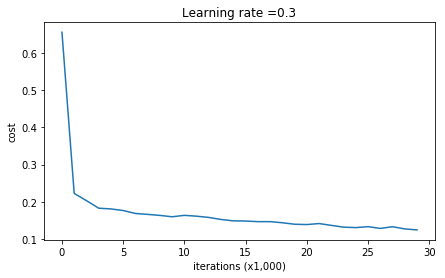
\includegraphics[width=0.6\textwidth]{course2/cost_without_regularization}
\end{center}
\end{figure}
\vspace{-0.7cm}
The train accuracy is 94.8\% while the test accuracy is 91.5\%. This is the {\textbf {baseline model}} (you will observe the impact of regularization on this model). Run the following code to plot the decision boundary of your model.

\begin{minted}{python}
plt.title("Model without regularization")
axes = plt.gca()
axes.set_xlim([-0.75,0.40])
axes.set_ylim([-0.75,0.65])
plot_decision_boundary(lambda x: predict_dec(parameters, x.T), train_X, train_Y)
\end{minted}
\vspace{-0.7cm}
\begin{figure}[h]
\begin{center}
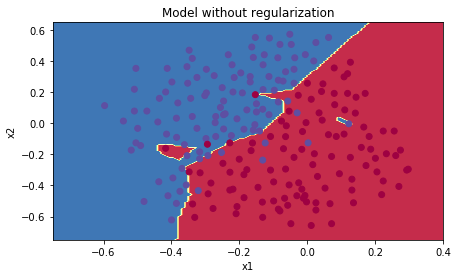
\includegraphics[width=0.6\textwidth]{course2/Model_without_regularization}
\caption{Model without regularization}
\end{center}
\end{figure}
\vspace{-0.7cm}

The non-regularized model is obviously overfitting the training set. It is fitting the noisy points! Lets now look at two techniques to reduce overfitting.



\subsubsubsection{L2 Regularization}

The standard way to avoid overfitting is called {\textbf {L2 regularization}}. It consists of appropriately modifying your cost function, from:
\begin{equation}
J = -\frac{1}{m} \sum\limits_{i = 1}^{m} \large{(}\small  y^{(i)}\log\left(a^{[L](i)}\right) + (1-y^{(i)})\log\left(1- a^{[L](i)}\right) \large{)} 
\end{equation}
To:
\begin{equation}\label{regularization}
J_{regularized} = \small \underbrace{-\frac{1}{m} \sum\limits_{i = 1}^{m} \large{(}\small y^{(i)}\log\left(a^{[L](i)}\right) + (1-y^{(i)})\log\left(1- a^{[L](i)}\right) \large{)} }_\text{cross-entropy cost} + \underbrace{\frac{1}{m} \frac{\lambda}{2} \sum\limits_l\sum\limits_k\sum\limits_j W_{k,j}^{[l]2} }_\text{L2 regularization cost} 
\end{equation}

Let's modify your cost and observe the consequences.

{\textbf {Exercise}}: Implement \emph{compute\_cost\_with\_regularization()} which computes the cost given by formula \eqref{regularization}. To calculate $\sum\limits_k\sum\limits_j W_{k,j}^{[l]2}$  , use :
\begin{minted}{python}
np.sum(np.square(Wl))
\end{minted}
Note that you have to do this for $W^{[1]}$, $W^{[2]}$ and $W^{[3]}$, then sum the three terms and multiply by $ \frac{1}{m} \frac{\lambda}{2} $.

\begin{minted}{python}
# GRADED FUNCTION: compute_cost_with_regularization
def compute_cost_with_regularization(A3, Y, parameters, lambd):
    """
    Implement the cost function with L2 regularization. See formula (2) above.
    
    Arguments:
    A3 -- post-activation, output of forward propagation, of shape (output size, number of examples)
    Y -- "true" labels vector, of shape (output size, number of examples)
    parameters -- python dictionary containing parameters of the model
    
    Returns:
    cost - value of the regularized loss function (formula (2))
    """
    m = Y.shape[1]
    W1 = parameters["W1"]
    W2 = parameters["W2"]
    W3 = parameters["W3"]
    
    cross_entropy_cost = compute_cost(A3, Y) # This gives you the cross-entropy part of the cost
    
    ### START CODE HERE ### (approx. 1 line)
    L2_regularization_cost = lambd * (np.sum(np.square(W1))+ np.sum(np.square(W2))+ np.sum(np.square(W3)))/(2*m) 
    ### END CODER HERE ###
    
    cost = cross_entropy_cost + L2_regularization_cost
    
    return cost
\end{minted}

\begin{minted}{python}
A3, Y_assess, parameters = compute_cost_with_regularization_test_case()

print("cost = " + str(compute_cost_with_regularization(A3, Y_assess, parameters, lambd = 0.1)))

#output
cost = 1.78648594516
\end{minted}


Of course, because you changed the cost, you have to change backward propagation as well! All the gradients have to be computed with respect to this new cost. 

{\textbf {Exercise}}: Implement the changes needed in backward propagation to take into account regularization. The changes only concern dW1, dW2 and dW3.{\textbf { For each, you have to add the regularization term's gradient ($\frac{d}{dW} ( \frac{1}{2}\frac{\lambda}{m}  W^2) = \frac{\lambda}{m} W$)}}.

\begin{minted}{python}
# GRADED FUNCTION: backward_propagation_with_regularization
def backward_propagation_with_regularization(X, Y, cache, lambd):
    """
    Implements the backward propagation of our baseline model to which we added an L2 regularization.
    
    Arguments:
    X -- input dataset, of shape (input size, number of examples)
    Y -- "true" labels vector, of shape (output size, number of examples)
    cache -- cache output from forward_propagation()
    lambd -- regularization hyperparameter, scalar
    
    Returns:
    gradients -- A dictionary with the gradients with respect to each parameter, activation and pre-activation variables
    """
    
    m = X.shape[1]
    (Z1, A1, W1, b1, Z2, A2, W2, b2, Z3, A3, W3, b3) = cache
    
    dZ3 = A3 - Y
    
    ### START CODE HERE ### (approx. 1 line)
    dW3 = 1./m * np.dot(dZ3, A2.T) + lambd*W3/m
    ### END CODE HERE ###
    db3 = 1./m * np.sum(dZ3, axis=1, keepdims = True)
    
    dA2 = np.dot(W3.T, dZ3)
    dZ2 = np.multiply(dA2, np.int64(A2 > 0))
    ### START CODE HERE ### (approx. 1 line)
    dW2 = 1./m * np.dot(dZ2, A1.T) + lambd*W2/m
    ### END CODE HERE ###
    db2 = 1./m * np.sum(dZ2, axis=1, keepdims = True)
    
    dA1 = np.dot(W2.T, dZ2)
    dZ1 = np.multiply(dA1, np.int64(A1 > 0))
    ### START CODE HERE ### (approx. 1 line)
    dW1 = 1./m * np.dot(dZ1, X.T) + lambd*W1/m
    ### END CODE HERE ###
    db1 = 1./m * np.sum(dZ1, axis=1, keepdims = True)
    
    gradients = {"dZ3": dZ3, "dW3": dW3, "db3": db3,"dA2": dA2,
                 "dZ2": dZ2, "dW2": dW2, "db2": db2, "dA1": dA1, 
                 "dZ1": dZ1, "dW1": dW1, "db1": db1}
    
    return gradients
\end{minted}

\begin{minted}{python}
X_assess, Y_assess, cache = backward_propagation_with_regularization_test_case()

grads = backward_propagation_with_regularization(X_assess, Y_assess, cache, lambd = 0.7)
print ("dW1 = "+ str(grads["dW1"]))
print ("dW2 = "+ str(grads["dW2"]))
print ("dW3 = "+ str(grads["dW3"]))

#output
dW1 = [[-0.25604646  0.12298827 -0.28297129]
 [-0.17706303  0.34536094 -0.4410571 ]]
dW2 = [[ 0.79276486  0.85133918]
 [-0.0957219  -0.01720463]
 [-0.13100772 -0.03750433]]
dW3 = [[-1.77691347 -0.11832879 -0.09397446]]

\end{minted}

Let's now run the model with L2 regularization $(\lambda = 0.7)$. The \emph{model()} function will call: 
\begin{itemize}
\item \emph{compute\_cost\_with\_regularization} instead of \emph{compute\_cost}
\item \emph{backward\_propagation\_with\_regularization} instead of \emph{backward\_propagation}
\end{itemize}

\begin{minted}{python}
parameters = model(train_X, train_Y, lambd = 0.7)
print ("On the train set:")
predictions_train = predict(train_X, train_Y, parameters)
print ("On the test set:")
predictions_test = predict(test_X, test_Y, parameters)

#output
Cost after iteration 0: 0.6974484493131264
Cost after iteration 10000: 0.2684918873282239
Cost after iteration 20000: 0.2680916337127301

#Accuracy
On the train set:
Accuracy: 0.938388625592
On the test set:
Accuracy: 0.93
\end{minted}

\vspace{-0.7cm}
\begin{figure}[h]
\begin{center}
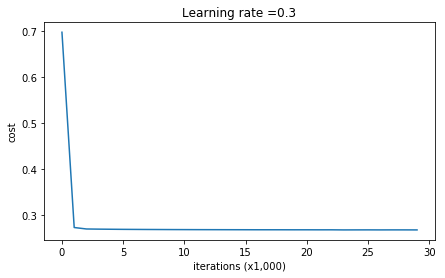
\includegraphics[width=0.7\textwidth]{course2/L2_regularization}
\end{center}
\end{figure}
\vspace{-0.7cm}

Congrats, the test set accuracy increased to 93\%. You have saved the French football team!

You are not overfitting the training data anymore. Let's plot the decision boundary.


\begin{figure}[h]
\begin{center}
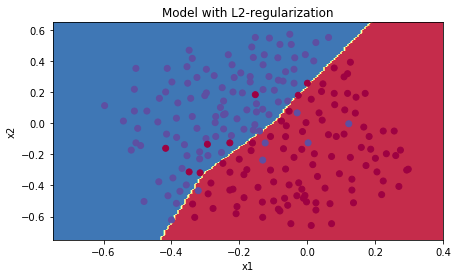
\includegraphics[width=0.7\textwidth]{course2/Model_with_L2_regularization}
\caption{Model with L2-regularization}
\end{center}
\end{figure}

\begin{minted}{python}
plt.title("Model with L2-regularization")
axes = plt.gca()
axes.set_xlim([-0.75,0.40])
axes.set_ylim([-0.75,0.65])
plot_decision_boundary(lambda x: predict_dec(parameters, x.T), train_X, train_Y)
\end{minted}


{\textbf {Observations}}:
\begin{itemize}
\item The value of $\lambda$ is a hyperparameter that you can tune using a dev set.
\item L2 regularization makes your decision boundary smoother. If $\lambda$ is too large, it is also possible to ``oversmooth", resulting in a model with high bias.
\end{itemize}
{\textbf {What is L2-regularization actually doing?}}:

L2-regularization relies on the assumption that a model with small weights is simpler than a model with large weights. Thus, by penalizing the square values of the weights in the cost function you drive all the weights to smaller values. It becomes too costly for the cost to have large weights! This leads to a smoother model in which the output changes more slowly as the input changes. 


{\color{red} {\textbf {What you should remember}} -- the implications of L2-regularization on:
\begin{itemize}
\item The cost computation:
    \begin{itemize}
    \item  A regularization term is added to the cost
    \end{itemize}
\item The backpropagation function:
    \begin{itemize}
    \item There are extra terms in the gradients with respect to weight matrices
    \end{itemize}
\item Weights end up smaller ("weight decay"): 
    \begin{itemize}
    \item Weights are pushed to smaller values.
    \end{itemize}
\end{itemize}
}

\clearpage
\subsubsubsection{Dropout}

Finally, {\textbf {dropout}} is a widely used regularization technique that is specific to deep learning. {\textbf {It randomly shuts down some neurons}} in each iteration. 
\begin{figure}[h]
\begin{center}
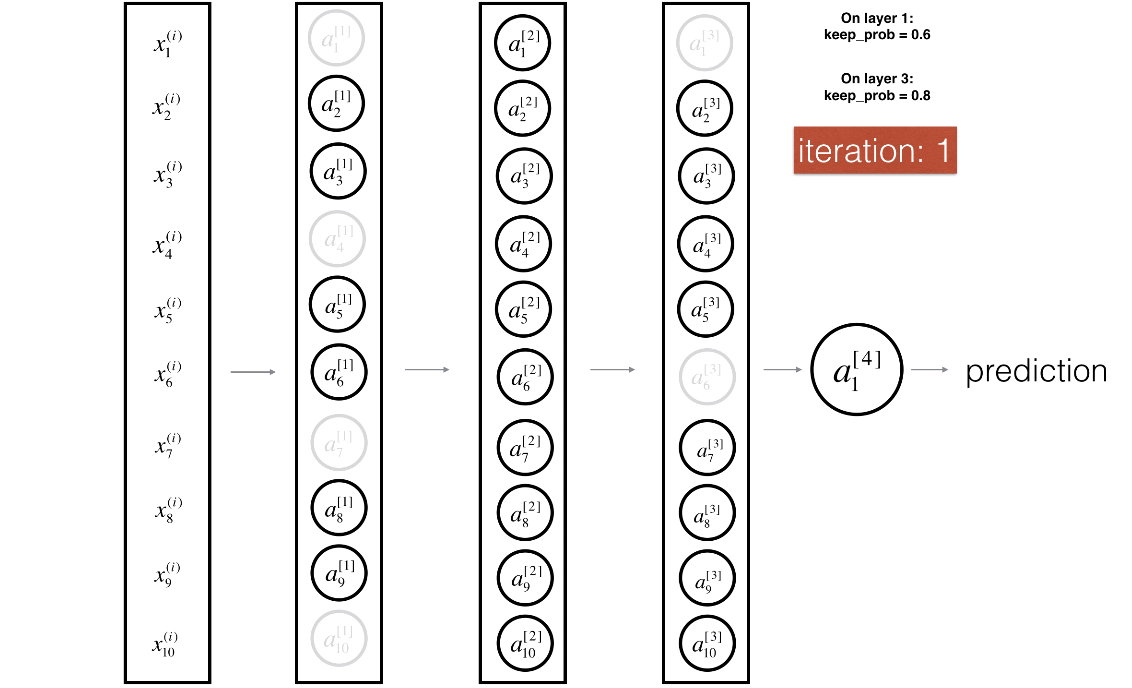
\includegraphics[width=0.9\textwidth]{course2/dropout}
\caption{Drop-out on the first and third hidden layers}
\end{center}
\end{figure}

At each iteration, you shut down (= set to zero) each neuron of a layer with probability  \emph{1−keep\_prob}  or keep it with probability  \emph{keep\_prob} (50\% here). The dropped neurons don't contribute to the training in both the forward and backward propagations of the iteration.

When you shut some neurons down, you actually modify your model. The idea behind drop-out is that at each iteration, you train a different model that uses only a subset of your neurons. With dropout, your neurons thus become less sensitive to the activation of one other specific neuron, because that other neuron might be shut down at any time.



\begin{tcolorbox}[title=Forward propagation with dropout]
{\textbf {Exercise}}: Implement the forward propagation with dropout. You are using a 3 layer neural network, and will add dropout to the first and second hidden layers. We will not apply dropout to the input layer or output layer. 

{\textbf {Instructions}}:
You would like to shut down some neurons in the first and second layers. To do that, you are going to carry out 4 Steps:
\begin{itemize}
\item[1.] In lecture, we dicussed creating a variable $d^{[1]}$ with the same shape as $a^{[1]}$ using 	``np.random.rand()'' to randomly get numbers between 0 and 1. Here, you will use a vectorized implementation, so create a random matrix $D^{[1]} = [d^{[1](1)} d^{[1](2)} ... d^{[1](m)}] $ of the same dimension as $A^{[1]}$.
\item[2.] Set each entry of $D^{[1]}$ to be 0 with probability (``1-keep\_prob'') or 1 with probability (``keep\_prob''), by thresholding values in $D^{[1]}$ appropriately. Hint: to set all the entries of a matrix X to 0 (if entry is less than 0.5) or 1 (if entry is more than 0.5) you would do: ``X = (X < 0.5)''. Note that 0 and 1 are respectively equivalent to False and True.
\item[3.] Set $A^{[1]}$ to $A^{[1]} * D^{[1]}$. (You are shutting down some neurons). You can think of $D^{[1]}$ as a mask, so that when it is multiplied with another matrix, it shuts down some of the values.
\item[4.] Divide $A^{[1]}$ by ``1-keep\_prob''. By doing this you are assuring that the result of the cost will still have the same expected value as without drop-out. (This technique is also called {\textbf {inverted dropout}}.)
\end{itemize}

\end{tcolorbox}

\begin{minted}{python}
# GRADED FUNCTION: forward_propagation_with_dropout
def forward_propagation_with_dropout(X, parameters, keep_prob = 0.5):
    """
    Implements the forward propagation: LINEAR -> RELU + DROPOUT -> LINEAR -> RELU + DROPOUT -> LINEAR -> SIGMOID.
    
    Arguments:
    X -- input dataset, of shape (2, number of examples)
    parameters -- python dictionary containing your parameters "W1", "b1", "W2", "b2", "W3", "b3":
                    W1 -- weight matrix of shape (20, 2)
                    b1 -- bias vector of shape (20, 1)
                    W2 -- weight matrix of shape (3, 20)
                    b2 -- bias vector of shape (3, 1)
                    W3 -- weight matrix of shape (1, 3)
                    b3 -- bias vector of shape (1, 1)
    keep_prob - probability of keeping a neuron active during drop-out, scalar
    
    Returns:
    A3 -- last activation value, output of the forward propagation, of shape (1,1)
    cache -- tuple, information stored for computing the backward propagation
    """
    
    np.random.seed(1)
    
    # retrieve parameters
    W1 = parameters["W1"]
    b1 = parameters["b1"]
    W2 = parameters["W2"]
    b2 = parameters["b2"]
    W3 = parameters["W3"]
    b3 = parameters["b3"]
    
    # LINEAR -> RELU -> LINEAR -> RELU -> LINEAR -> SIGMOID
    Z1 = np.dot(W1, X) + b1
    A1 = relu(Z1)
    ### START CODE HERE ### (approx. 4 lines)         # Steps 1-4 below correspond to the Steps 1-4 described above. 
    D1 = np.random.rand(A1.shape[0], A1.shape[1])     # Step 1: initialize matrix D1 = np.random.rand(..., ...)
    D1 = ( D1 < keep_prob)                            # Step 2: convert entries of D1 to 0 or 1 (using keep_prob as the threshold)
    A1 = A1 * D1                                      # Step 3: shut down some neurons of A1
    A1 = A1/keep_prob                                 # Step 4: scale the value of neurons that haven't been shut down
    ### END CODE HERE ###
    Z2 = np.dot(W2, A1) + b2
    A2 = relu(Z2)
    ### START CODE HERE ### (approx. 4 lines)
    D2 = np.random.rand(A2.shape[0], A2.shape[1])     # Step 1: initialize matrix D2 = np.random.rand(..., ...)
    D2 = ( D2 < keep_prob )                           # Step 2: convert entries of D2 to 0 or 1 (using keep_prob as the threshold)
    A2 = A2 * D2                                      # Step 3: shut down some neurons of A2
    A2 = A2/keep_prob                                 # Step 4: scale the value of neurons that haven't been shut down
    ### END CODE HERE ###
    Z3 = np.dot(W3, A2) + b3
    A3 = sigmoid(Z3)
    
    cache = (Z1, D1, A1, W1, b1, Z2, D2, A2, W2, b2, Z3, A3, W3, b3)
    
    return A3, cache
\end{minted}


\begin{minted}{python}
X_assess, parameters = forward_propagation_with_dropout_test_case()

A3, cache = forward_propagation_with_dropout(X_assess, parameters, keep_prob = 0.7)
print ("A3 = " + str(A3))

#output
A3 = [[ 0.36974721  0.00305176  0.04565099  0.49683389  0.36974721]]
\end{minted}



\begin{tcolorbox}[title=Backward propagation with dropout]
{\textbf {Exercise}}: Implement the backward propagation with dropout. As before, you are training a 3 layer network. Add dropout to the first and second hidden layers, using the masks $D^{[1]}$ and $D^{[2]}$ stored in the cache. 

{\textbf {Instruction}}:
Backpropagation with dropout is actually quite easy. You will have to carry out 2 Steps:
\begin{itemize}
\item[1.] You had previously shut down some neurons during forward propagation, by applying a mask $D^{[1]}$ to ``A1''. In backpropagation, you will have to shut down the same neurons, by reapplying the same mask $D^{[1]}$ to ``dA1''. 
\item[2.] During forward propagation, you had divided ``A1'' by ``keep\_prob''. In backpropagation, you'll therefore have to divide ``dA1'' by ``keep\_prob'' again (the calculus interpretation is that if $A^{[1]}$ is scaled by ``keep\_prob'', then its derivative $dA^{[1]}$ is also scaled by the same ``keep\_prob'').
\end{itemize}
\end{tcolorbox}

\begin{minted}{python}
# GRADED FUNCTION: backward_propagation_with_dropout
def backward_propagation_with_dropout(X, Y, cache, keep_prob):
    """
    Implements the backward propagation of our baseline model to which we added dropout.
    
    Arguments:
    X -- input dataset, of shape (2, number of examples)
    Y -- "true" labels vector, of shape (output size, number of examples)
    cache -- cache output from forward_propagation_with_dropout()
    keep_prob - probability of keeping a neuron active during drop-out, scalar
    
    Returns:
    gradients -- A dictionary with the gradients with respect to each parameter, activation and pre-activation variables
    """
    
    m = X.shape[1]
    (Z1, D1, A1, W1, b1, Z2, D2, A2, W2, b2, Z3, A3, W3, b3) = cache
    
    dZ3 = A3 - Y
    dW3 = 1./m * np.dot(dZ3, A2.T)
    db3 = 1./m * np.sum(dZ3, axis=1, keepdims = True)
    dA2 = np.dot(W3.T, dZ3)
    ### START CODE HERE ### (≈ 2 lines of code)
    dA2 = dA2 * D2              # Step 1: Apply mask D2 to shut down the same neurons as during the forward propagation
    dA2 = dA2/keep_prob         # Step 2: Scale the value of neurons that haven't been shut down
    ### END CODE HERE ###
    dZ2 = np.multiply(dA2, np.int64(A2 > 0))
    dW2 = 1./m * np.dot(dZ2, A1.T)
    db2 = 1./m * np.sum(dZ2, axis=1, keepdims = True)
    
    dA1 = np.dot(W2.T, dZ2)
    ### START CODE HERE ### (≈ 2 lines of code)
    dA1 = dA1 * D1              # Step 1: Apply mask D1 to shut down the same neurons as during the forward propagation
    dA1 = dA1/keep_prob              # Step 2: Scale the value of neurons that haven't been shut down
    ### END CODE HERE ###
    dZ1 = np.multiply(dA1, np.int64(A1 > 0))
    dW1 = 1./m * np.dot(dZ1, X.T)
    db1 = 1./m * np.sum(dZ1, axis=1, keepdims = True)
    
    gradients = {"dZ3": dZ3, "dW3": dW3, "db3": db3,"dA2": dA2,
                 "dZ2": dZ2, "dW2": dW2, "db2": db2, "dA1": dA1, 
                 "dZ1": dZ1, "dW1": dW1, "db1": db1}
    
    return gradients
\end{minted}

\begin{minted}{python}
#output
dA1 = [[ 0.36544439  0.         -0.00188233  0.         -0.17408748]
 [ 0.65515713  0.         -0.00337459  0.         -0.        ]]
dA2 = [[ 0.58180856  0.         -0.00299679  0.         -0.27715731]
 [ 0.          0.53159854 -0.          0.53159854 -0.34089673]
 [ 0.          0.         -0.00292733  0.         -0.        ]]

\end{minted}

Let's now run the model with dropout (keep\_prob = 0.86). It means at every iteration you shut down each neurons of layer 1 and 2 with 24\% probability. The function model() will now call:
\begin{itemize}
\item forward\_propagation\_with\_dropout instead of forward\_propagation.
\item backward\_propagation\_with\_dropout instead of backward\_propagation.
\end{itemize}

\begin{minted}{python}
parameters = model(train_X, train_Y, keep_prob = 0.86, learning_rate = 0.3)

print ("On the train set:")
predictions_train = predict(train_X, train_Y, parameters)
print ("On the test set:")
predictions_test = predict(test_X, test_Y, parameters)

#output
Cost after iteration 0: 0.6543912405149825
Cost after iteration 10000: 0.06101698657490559
Cost after iteration 20000: 0.060582435798513114

#Accuracy:
On the train set:
Accuracy: 0.928909952607
On the test set:
Accuracy: 0.95
\end{minted}
\clearpage

\begin{figure}[h]
\begin{center}
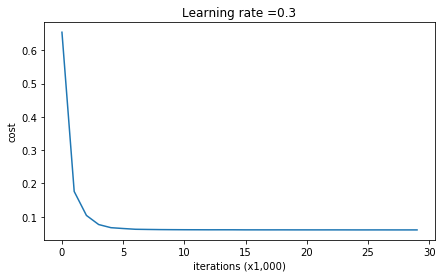
\includegraphics[width=0.8\textwidth]{course2/cost_dropout}
\end{center}
\end{figure}


Dropout works great! The test accuracy has increased again (to 95\%)! Your model is not overfitting the training set and does a great job on the test set. The French football team will be forever grateful to you!

Run the code below to plot the decision boundary.
\begin{minted}{python}
plt.title("Model with dropout")
axes = plt.gca()
axes.set_xlim([-0.75,0.40])
axes.set_ylim([-0.75,0.65])
plot_decision_boundary(lambda x: predict_dec(parameters, x.T), train_X, train_Y)
\end{minted}

\begin{figure}[h]
\begin{center}
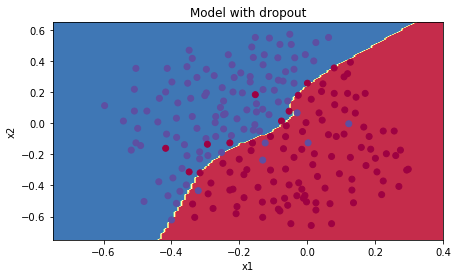
\includegraphics[width=0.8\textwidth]{course2/Model_with_dropout}
\caption{Model with dropout}
\end{center}
\end{figure}

{\textbf {Note}}:
\begin{itemize}
\item A {\textbf {common mistake}} when using dropout is to use it both in training and testing. You should use dropout (randomly eliminate nodes) only in training. 
\item Deep learning frameworks like \href{https://www.tensorflow.org/api_docs/python/tf/nn/dropout}{tensorflow}, \href{http://doc.paddlepaddle.org/release_doc/0.9.0/doc/ui/api/trainer_config_helpers/attrs.html}{PaddlePaddle}, \href{https://keras.io/layers/core/\#dropout)}{keras} or \href{http://caffe.berkeleyvision.org/tutorial/layers/dropout.html}{caffe} come with a dropout layer implementation. Don't stress - you will soon learn some of these frameworks.
\end{itemize}

{\color{red}{\textbf {What you should remember about dropout}}:
\begin{itemize}
\item Dropout is a regularization technique.
\item You only use dropout during training. Don't use dropout (randomly eliminate nodes) during test time.
\item Apply dropout both during forward and backward propagation.
\item During training time, divide each dropout layer by keep\_prob to keep the same expected value for the activations. For example, if keep\_prob is 0.5, then we will on average shut down half the nodes, so the output will be scaled by 0.5 since only the remaining half are contributing to the solution. Dividing by 0.5 is equivalent to multiplying by 2. Hence, the output now has the same expected value. You can check that this works even when keep\_prob is other values than 0.5.  
\end{itemize}
}

\subsubsubsection{Conclusions}

{\textbf {Here are the results of our three models:}}
\begin{table}[H]
\centering
\begin{tabular}{ccc}  
\toprule
model	&train accuracy	 &test accuracy\\
\midrule
3-layer NN without regularization&	95\%	&91.5\%\\
3-layer NN with L2-regularization&	94\%	&93\%\\
3-layer NN with dropout&	93\%	&95\%\\
\bottomrule
\end{tabular}
\end{table}

Note that regularization hurts training set performance! This is because it limits the ability of the network to overfit to the training set. But since it ultimately gives better test accuracy, it is helping your system.

Congratulations for finishing this assignment! And also for revolutionizing French football. :-)


{\color{red}{\textbf {What you should remember in this assignmnet}}:
\begin{itemize}
\item Regularization will help you reduce overfitting.
\item Regularization will drive your weights to lower values.
\item L2 regularization and Dropout are two very effective regularization techniques.
\end{itemize}
}

\clearpage
\subsubsection{Gradient Checking}

Welcome to this week's third programming assignment! You will be implementing gradient checking to make sure that your backpropagation implementation is correct.

You are part of a team working to make mobile payments available globally, and are asked to build a deep learning model to detect fraud--whenever someone makes a payment, you want to see if the payment might be fraudulent, such as if the user's account has been taken over by a hacker.

But backpropagation is quite challenging to implement, and sometimes has bugs. Because this is a mission-critical application, your company's CEO wants to be really certain that your implementation of backpropagation is correct. Your CEO says, ``Give me a proof that your backpropagation is actually working!" To give this reassurance, you are going to use ``gradient checking".


By completing this assignment you will:
\begin{itemize}
\item Implement gradient checking from scratch.
\item Understand how to use the difference formula to check your backpropagation implementation.
\item Recognize that your backpropagation algorithm should give you similar results as the ones you got by computing the difference formula.
\item Learn how to identify which parameter's gradient was computed incorrectly.
\end{itemize}

Take your time to complete this assignment, and make sure you get the expected outputs when working through the different exercises. In some code blocks, you will find a ``\#GRADED FUNCTION: functionName" comment. Please do not modify it. After you are done, submit your work and check your results. You need to score 80\% to pass. Good luck :) !

Let's do it!


\subsubsubsection{How does gradient checking work?}\label{sec:1}

Backpropagation computes the gradients $\frac{\partial J}{\partial \theta}$, where $\theta$ denotes the parameters of the model. $J$ is computed using forward propagation and your loss function.

Because forward propagation is relatively easy to implement, you're confident you got that right, and so you're almost  100\% sure that you're computing the cost $J$ correctly. Thus, you can use your code for computing $J$ to verify the code for computing $\frac{\partial J}{\partial \theta}$. 

Let's look back at the definition of a derivative (or gradient):
\begin{equation}\label{eq:gradient}
\frac{\partial J}{\partial \theta} = \lim_{\varepsilon \to 0} \frac{J(\theta + \varepsilon) - J(\theta - \varepsilon)}{2 \varepsilon} \end{equation}

If you're not familiar with the ``$\displaystyle \lim_{\varepsilon \to 0}$" notation, it's just a way of saying ``when $\varepsilon$ is really really small."

We know the following:
\begin{itemize}
\item  $\frac{\partial J}{\partial \theta}$ is what you want to make sure you're computing correctly. 
\item You can compute $J(\theta + \varepsilon)$ and $J(\theta - \varepsilon)$ (in the case that $\theta$ is a real number), since you're confident your implementation for $J$ is correct. 
\end{itemize}

Lets use equation \eqref{eq:gradient} and a small value for $\varepsilon$ to convince your CEO that your code for computing  $\frac{\partial J}{\partial \theta}$ is correct!


\subsubsubsection{1-dimensional gradient checking}\label{sec:2}

Consider a 1D linear function $J(\theta) = \theta x$. The model contains only a single real-valued parameter $\theta$, and takes $x$ as input.

You will implement code to compute $J(.)$ and its derivative $\frac{\partial J}{\partial \theta}$. You will then use gradient checking to make sure your derivative computation for $J$ is correct. 

\begin{figure}[h]
\begin{center}
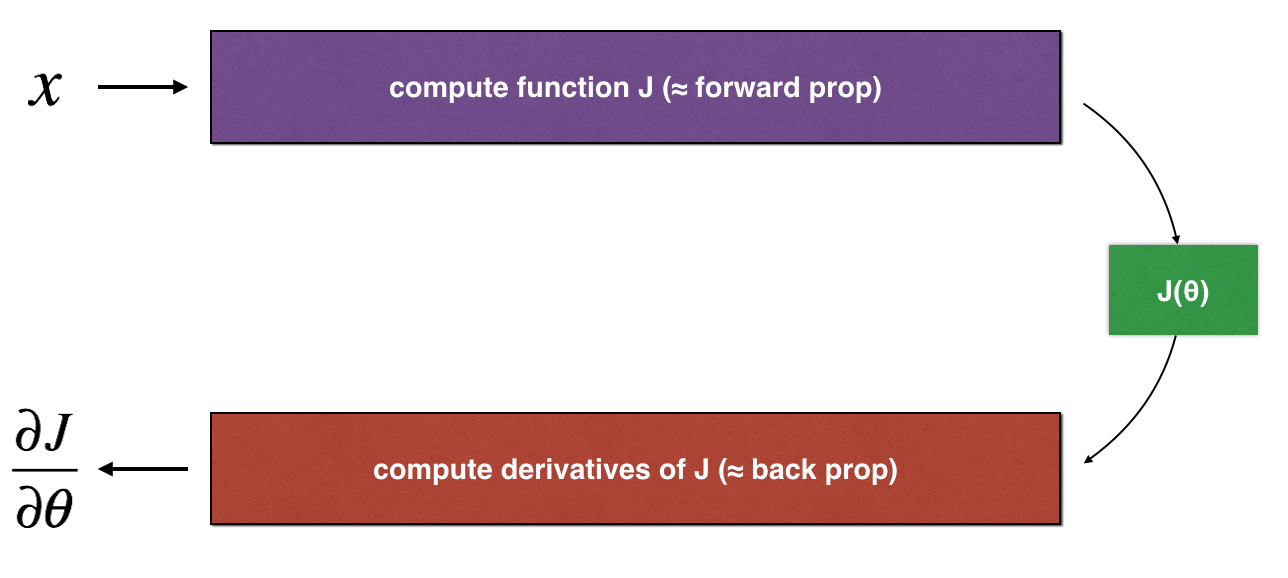
\includegraphics[width=0.8\textwidth]{course2/1-dimensional_gradient_checking}
\caption{1D linear model}
\label{1-dimensional}
\end{center}
\end{figure}

The diagram above shows the key computation steps: First start with $x$, then evaluate the function $J(x)$ (``forward propagation"). Then compute the derivative $\frac{\partial J}{\partial \theta}$ (``backward propagation"). 

{\textbf {Exercise}}: implement ``forward propagation" and ``backward propagation" for this simple function. I.e., compute both $J(.)$ (``forward propagation") and its derivative with respect to $\theta$ (``backward propagation"), in two separate functions. 


\begin{minted}{python}
# GRADED FUNCTION: forward_propagation
def forward_propagation(x, theta):
    """
    Implement the linear forward propagation (compute J) presented in Figure 1 (J(theta) = theta * x)
    
    Arguments:
    x -- a real-valued input
    theta -- our parameter, a real number as well
    
    Returns:
    J -- the value of function J, computed using the formula J(theta) = theta * x
    """
    
    ### START CODE HERE ### (approx. 1 line)
    J = theta * x
    ### END CODE HERE ###
    
    return J
\end{minted}
\begin{minted}{python}
x, theta = 2, 4
J = forward_propagation(x, theta)
print ("J = " + str(J))

#output
J=8
\end{minted}


{\textbf {Exercise}}: Now, implement the backward propagation step (derivative computation) of Figure \ref{1-dimensional}. That is, compute the derivative of $J(\theta) = \theta x$ with respect to $\theta$. To save you from doing the calculus, you should get $dtheta = \frac { \partial J }{ \partial \theta} = x$.
\begin{minted}{python}
# GRADED FUNCTION: backward_propagation
def backward_propagation(x, theta):
    """
    Computes the derivative of J with respect to theta (see Figure).
    
    Arguments:
    x -- a real-valued input
    theta -- our parameter, a real number as well
    
    Returns:
    dtheta -- the gradient of the cost with respect to theta
    """
    
    ### START CODE HERE ### (approx. 1 line)
    dtheta = x
    ### END CODE HERE ###
    
    return dtheta
\end{minted}

\begin{minted}{python}
x, theta = 2, 4
dtheta = backward_propagation(x, theta)
print ("dtheta = " + str(dtheta))

#output
dtheta = 2
\end{minted}



{\textbf {Exercise}}: To show that the \emph{backward\_propagation()} function is correctly computing the gradient $\frac{\partial J}{\partial \theta}$, let's implement gradient checking.

{\textbf {Instructions}}:
\begin{itemize}
\item First compute ``gradapprox" using the formula above \eqref{eq:gradient} and a small value of $\varepsilon$. Here are the Steps to follow:
    \begin{itemize}
    \item[1.] $\theta^{+} = \theta + \varepsilon$
    \item[2.] $\theta^{-} = \theta - \varepsilon$
    \item[3.] $J^{+} = J(\theta^{+})$
    \item[4.] $J^{-} = J(\theta^{-})$
    \item[5.] $gradapprox = \frac{J^{+} - J^{-}}{2  \varepsilon}$
    \end{itemize}
\item Then compute the gradient using backward propagation, and store the result in a variable ``grad"
\item Finally, compute the relative difference between ``gradapprox" and the ``grad" using the following formula:
\begin{equation}
difference = \frac {\mid\mid grad - gradapprox \mid\mid_2}{\mid\mid grad \mid\mid_2 + \mid\mid gradapprox \mid\mid_2}
\end{equation}
\end{itemize}

You will need 3 Steps to compute this formula:
\begin{itemize}
\item[1]. compute the numerator using np.linalg.norm(...)
\item[2]. compute the denominator. You will need to call np.linalg.norm(...) twice.
\item[3]. divide them.
\end{itemize}

If this difference is small (say less than $10^{-7}$), you can be quite confident that you have computed your gradient correctly. Otherwise, there may be a mistake in the gradient computation. 

\begin{minted}{python}
# GRADED FUNCTION: gradient_check
def gradient_check(x, theta, epsilon = 1e-7):
    """
    Implement the backward propagation presented in Figure 1.
    
    Arguments:
    x -- a real-valued input
    theta -- our parameter, a real number as well
    epsilon -- tiny shift to the input to compute approximated gradient with formula(1)
    
    Returns:
    difference -- difference (2) between the approximated gradient and the backward propagation gradient
    """
    
    # Compute gradapprox using left side of formula (1). epsilon is small enough, you don't need to worry about the limit.
    ### START CODE HERE ### (approx. 5 lines)
    thetaplus = theta + epsilon          # Step 1
    thetaminus = theta - epsilon         # Step 2
    J_plus = thetaplus * x               # Step 3
    J_minus = thetaminus * x             # Step 4
    gradapprox = ( J_plus-J_minus)/(2*epsilon)  # Step 5
    ### END CODE HERE ###
    
    # Check if gradapprox is close enough to the output of backward_propagation()
    ### START CODE HERE ### (approx. 1 line)
    grad = backward_propagation(x, theta)
    ### END CODE HERE ###
    
    ### START CODE HERE ### (approx. 1 line)
    numerator = np.linalg.norm(grad-gradapprox)             # Step 1'
    denominator = np.linalg.norm(grad) + np.linalg.norm(gradapprox) # Step 2'
    difference = numerator/denominator                              # Step 3'
    ### END CODE HERE ###
    
    if difference < 1e-7:
        print ("The gradient is correct!")
    else:
        print ("The gradient is wrong!")
    
    return difference
\end{minted}    

\begin{minted}{python}
x, theta = 2, 4
difference = gradient_check(x, theta)
print("difference = " + str(difference))

#output
The gradient is correct!
difference = 2.91933588329e-10
\end{minted}    


Congrats, the difference is smaller than the $10^{-7}$ threshold. So you can have high confidence that you've correctly computed the gradient in \emph{backward\_propagation()}. 

Now, in the more general case, your cost function $J$ has more than a single 1D input. When you are training a neural network, $\theta$ actually consists of multiple matrices $W^{[l]}$ and biases $b^{[l]}$! It is important to know how to do a gradient check with higher-dimensional inputs. Let's do it!


\subsubsubsection{N-dimensional gradient checking}

The following figure \ref{N-dimensional} describes the forward and backward propagation of your fraud detection model.
\clearpage
\begin{figure}[h]
\begin{center}
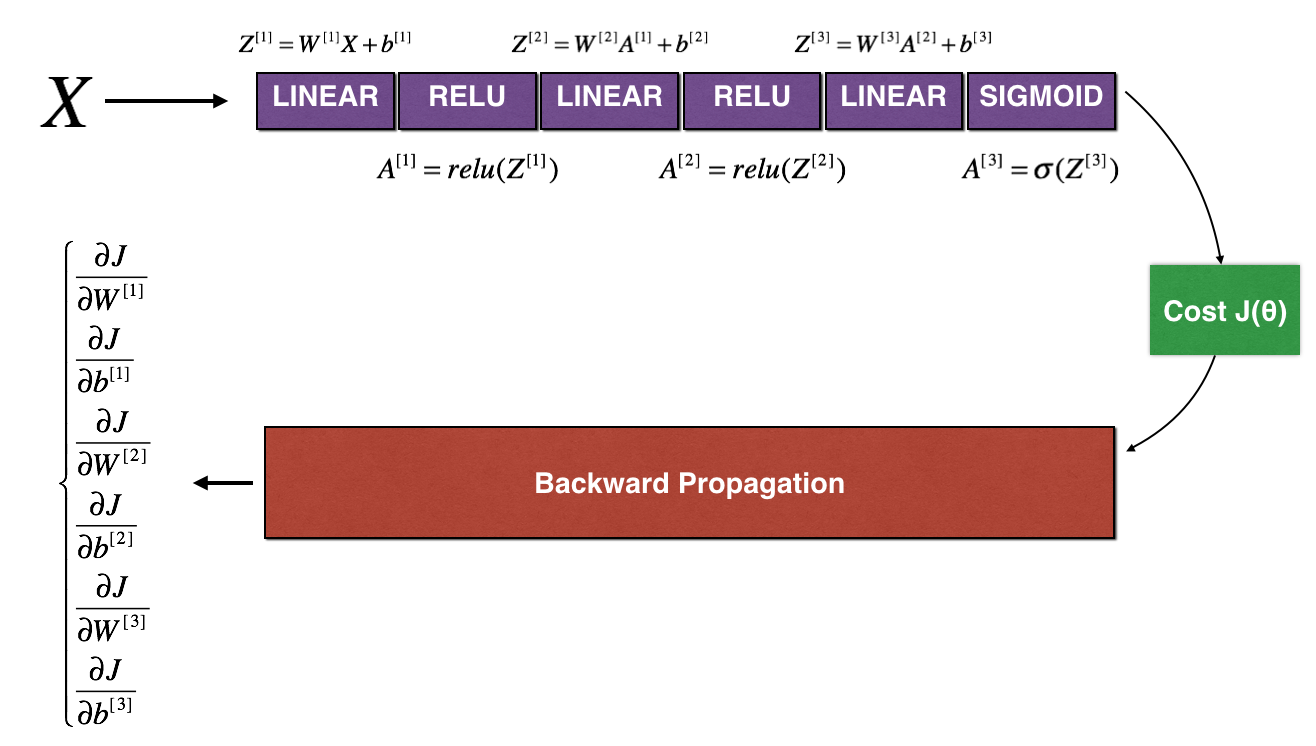
\includegraphics[width=0.8\textwidth]{course2/N-dimensional}
\caption{deep neural network(LINEAR -> RELU -> LINEAR -> RELU -> LINEAR -> SIGMOID)}
\label{N-dimensional}
\end{center}
\end{figure}

Let's look at your implementations for forward propagation and backward propagation.

\begin{minted}{python}
def forward_propagation_n(X, Y, parameters):
    """
    Implements the forward propagation (and computes the cost) presented in Figure 3.
    
    Arguments:
    X -- training set for m examples
    Y -- labels for m examples 
    parameters -- python dictionary containing your parameters "W1", "b1", "W2", "b2", "W3", "b3":
                    W1 -- weight matrix of shape (5, 4)
                    b1 -- bias vector of shape (5, 1)
                    W2 -- weight matrix of shape (3, 5)
                    b2 -- bias vector of shape (3, 1)
                    W3 -- weight matrix of shape (1, 3)
                    b3 -- bias vector of shape (1, 1)
    
    Returns:
    cost -- the cost function (logistic cost for one example)
    """
    
    # retrieve parameters
    m = X.shape[1]
    W1 = parameters["W1"]
    b1 = parameters["b1"]
    W2 = parameters["W2"]
    b2 = parameters["b2"]
    W3 = parameters["W3"]
    b3 = parameters["b3"]

    # LINEAR -> RELU -> LINEAR -> RELU -> LINEAR -> SIGMOID
    Z1 = np.dot(W1, X) + b1
    A1 = relu(Z1)
    Z2 = np.dot(W2, A1) + b2
    A2 = relu(Z2)
    Z3 = np.dot(W3, A2) + b3
    A3 = sigmoid(Z3)

    # Cost
    logprobs = np.multiply(-np.log(A3),Y) + np.multiply(-np.log(1 - A3), 1 - Y)
    cost = 1./m * np.sum(logprobs)
    
    cache = (Z1, A1, W1, b1, Z2, A2, W2, b2, Z3, A3, W3, b3)
    
    return cost, cache
\end{minted}

Now, run backward propagation.

\begin{minted}{python}
def backward_propagation_n(X, Y, cache):
    """
    Implement the backward propagation presented in figure 2.
    
    Arguments:
    X -- input datapoint, of shape (input size, 1)
    Y -- true "label"
    cache -- cache output from forward_propagation_n()
    
    Returns:
    gradients -- A dictionary with the gradients of the cost with respect to each parameter, activation and pre-activation variables.
    """
    
    m = X.shape[1]
    (Z1, A1, W1, b1, Z2, A2, W2, b2, Z3, A3, W3, b3) = cache
    
    dZ3 = A3 - Y
    dW3 = 1./m * np.dot(dZ3, A2.T)
    db3 = 1./m * np.sum(dZ3, axis=1, keepdims = True)
    
    dA2 = np.dot(W3.T, dZ3)
    dZ2 = np.multiply(dA2, np.int64(A2 > 0))
    dW2 = 1./m * np.dot(dZ2, A1.T) * 2
    db2 = 1./m * np.sum(dZ2, axis=1, keepdims = True)
    
    dA1 = np.dot(W2.T, dZ2)
    dZ1 = np.multiply(dA1, np.int64(A1 > 0))
    dW1 = 1./m * np.dot(dZ1, X.T)
    db1 = 4./m * np.sum(dZ1, axis=1, keepdims = True)
    
    gradients = {"dZ3": dZ3, "dW3": dW3, "db3": db3,
                 "dA2": dA2, "dZ2": dZ2, "dW2": dW2, "db2": db2,
                 "dA1": dA1, "dZ1": dZ1, "dW1": dW1, "db1": db1}
    
    return gradients
\end{minted} 

You obtained some results on the fraud detection test set but you are not 100\% sure of your model. Nobody's perfect! Let's implement gradient checking to verify if your gradients are correct.

{\textbf {How does gradient checking work?}}.

As in \ref{sec:1} and \ref{sec:2}, you want to compare ``gradapprox" to the gradient computed by backpropagation. The formula is \eqref{eq:gradient}, as follows:

\begin{equation*}
\frac{\partial J}{\partial \theta} = \lim_{\varepsilon \to 0} \frac{J(\theta + \varepsilon) - J(\theta - \varepsilon)}{2 \varepsilon} \end{equation*}

However, $\theta$ is not a scalar anymore. It is a dictionary called ``parameters". We implemented a function ``dictionary\_to\_vector()" for you. It converts the ``parameters" dictionary into a vector called ``values", obtained by reshaping all parameters (W1, b1, W2, b2, W3, b3) into vectors and concatenating them.

The inverse function is ``vector\_to\_dictionary" which outputs back the ``parameters" dictionary.

\begin{figure}[h]
\begin{center}
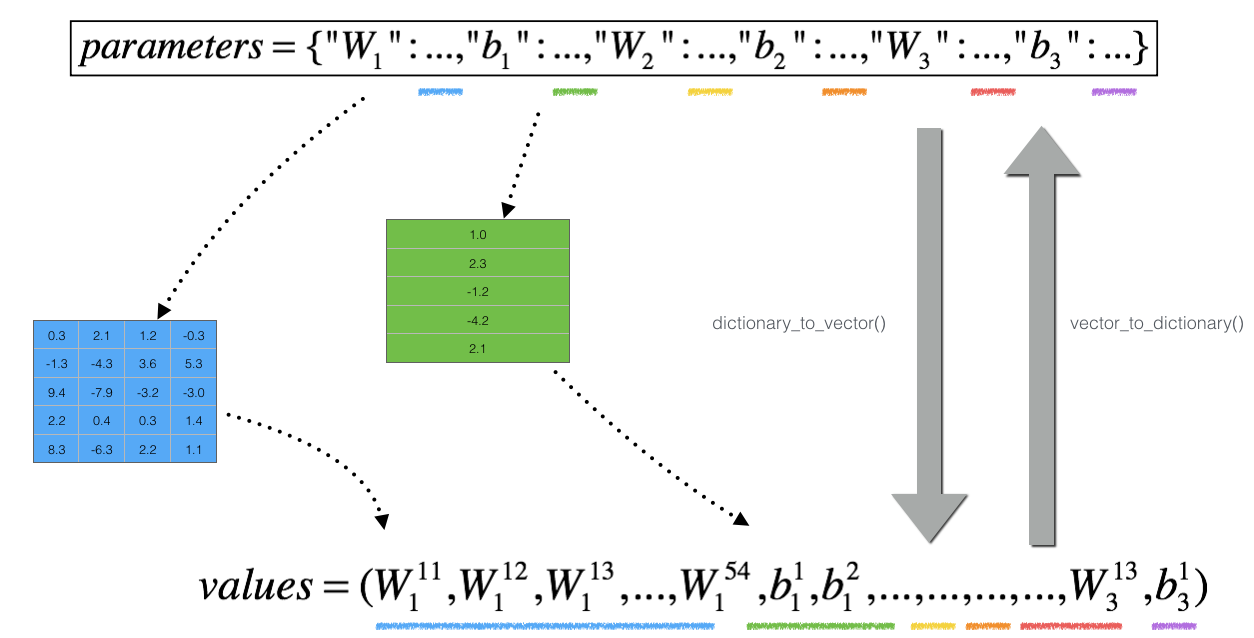
\includegraphics[width=0.8\textwidth]{course2/dictionary_vector}
\caption{dictionary\_to\_vector() and vector\_to\_dictionary()}
\label{dictionary_to_vector}
\end{center}
\end{figure}


We have also converted the ``gradients" dictionary into a vector ``grad" using gradients\_to\_vector(). You don't need to worry about that.

{\textbf {Exercise}}: Implement gradient\_check\_n().

{\textbf {Instructions}}: Here is pseudo-code that will help you implement the gradient check.


\begin{algorithm}[H]
\caption{N-dimensional gradient checking}
\begin{algorithmic}[1]
  \For{i in num\_parameters}
  \State Calculate: J\_plus[i]
  \State \hspace{0.5cm} Set $\theta^{+}$ to np.copy(parameters\_values)
  \State \hspace{0.5cm} Set $\theta^{+}_i$ to $\theta^{+}_i + \varepsilon$
  \State \hspace{0.5cm} Calculate $J^{+}_i$ using to forward\_propagation\_n(x, y, vector\_to\_dictionary($\theta^{+}$ ))
  \State Calculate J\_minus[i]:
  \State \hspace{0.5cm} do the same thing with $\theta^{-}$
  \State Compute $gradapprox[i] = \frac{J^{+}_i - J^{-}_i}{2 \varepsilon}$
  \EndFor
\end{algorithmic}
\end{algorithm}


Thus, you get a vector gradapprox, where gradapprox[i] is an approximation of the gradient with respect to parameter\_values[i]. You can now compare this gradapprox vector to the gradients vector from backpropagation. Just like for the 1D case (Steps 1, 2, 3), compute:
\begin{equation}
difference = \frac {\| grad - gradapprox \|_2}{\| grad \|_2 + \| gradapprox \|_2 }
\end{equation}

\begin{minted}{python}
# GRADED FUNCTION: gradient_check_n
def gradient_check_n(parameters, gradients, X, Y, epsilon = 1e-7):
    """
    Checks if backward_propagation_n computes correctly the gradient of the cost output by forward_propagation_n
    
    Arguments:
    parameters -- python dictionary containing your parameters "W1", "b1", "W2", "b2", "W3", "b3":
    grad -- output of backward_propagation_n, contains gradients of the cost with respect to the parameters. 
    x -- input datapoint, of shape (input size, 1)
    y -- true "label"
    epsilon -- tiny shift to the input to compute approximated gradient with formula(1)
    
    Returns:
    difference -- difference (2) between the approximated gradient and the backward propagation gradient
    """
    
    # Set-up variables
    parameters_values, _ = dictionary_to_vector(parameters)
    grad = gradients_to_vector(gradients)
    num_parameters = parameters_values.shape[0]
    J_plus = np.zeros((num_parameters, 1))
    J_minus = np.zeros((num_parameters, 1))
    gradapprox = np.zeros((num_parameters, 1))
    
    # Compute gradapprox
    for i in range(num_parameters):
        
        # Compute J_plus[i]. Inputs: "parameters_values, epsilon". Output = "J_plus[i]".
        # "_" is used because the function you have to outputs two parameters but we only care about the first one
        ### START CODE HERE ### (approx. 3 lines)
        thetaplus = np.copy(parameters_values)        # Step 1
        thetaplus[i][0] = thetaplus[i][0] + epsilon   # Step 2
        J_plus[i], _ = forward_propagation_n(X, Y, vector_to_dictionary(thetaplus))   # Step 3
        ### END CODE HERE ###

        # Compute J_minus[i]. Inputs: "parameters_values, epsilon". Output = "J_minus[i]".
        ### START CODE HERE ### (approx. 3 lines)
        thetaminus = np.copy(parameters_values)      # Step 1
        thetaminus[i][0] = thetaminus[i][0] - epsilon  # Step 2        
        J_minus[i], _ = forward_propagation_n(X, Y, vector_to_dictionary(thetaminus)) # Step 3
        ### END CODE HERE ###

        # Compute gradapprox[i]
        ### START CODE HERE ### (approx. 1 line)
        gradapprox[i] = (J_plus[i] - J_minus[i]) / (2.* epsilon)
        ### END CODE HERE ###

    # Compare gradapprox to backward propagation gradients by computing difference.
    ### START CODE HERE ### (approx. 1 line)
    numerator = np.linalg.norm(grad - gradapprox)        # Step 1'
    denominator = np.linalg.norm(grad) + np.linalg.norm(gradapprox)  # Step 2'
    difference = numerator / denominator    # Step 3'
    ### END CODE HERE ###

    if difference > 1e-7:
        print ("\033[93m" + "There is a mistake in the backward propagation! difference = " + str(difference) + "\033[0m")
    else:
        print ("\033[92m" + "Your backward propagation works perfectly fine! difference = " + str(difference) + "\033[0m")
    
    return difference
\end{minted}

\begin{minted}{python}
X, Y, parameters = gradient_check_n_test_case()

cost, cache = forward_propagation_n(X, Y, parameters)
gradients = backward_propagation_n(X, Y, cache)
difference = gradient_check_n(parameters, gradients, X, Y)

#output
There is a mistake in the backward propagation! difference = 0.285093156781
\end{minted}


It seems that there were errors in the \emph{backward\_propagation\_n} code we gave you! Good that you've implemented the gradient check. Go back to \emph{backward\_propagation} and try to find/correct the errors {\color{red} (Hint: check dW2 and db1)}. Rerun the gradient check when you think you've fixed it. Remember you'll need to re-execute the cell defining \emph{backward\_propagation\_n()} if you modify the code. 

Can you get gradient check to declare your derivative computation correct? Even though this part of the assignment isn't graded, we strongly urge you to try to find the bug and re-run gradient check until you're convinced backprop is now correctly implemented. 

{\textbf{Note}}
\begin{itemize}
\item Gradient Checking is slow! Approximating the gradient with $\frac{\partial J}{\partial \theta} \approx  \frac{J(\theta + \varepsilon) - J(\theta - \varepsilon)}{2 \varepsilon}$ is computationally costly. For this reason, we don't run gradient checking at every iteration during training. Just a few times to check if the gradient is correct. 
\item Gradient Checking, at least as we've presented it, doesn't work with dropout. You would usually run the gradient check algorithm without dropout to make sure your backprop is correct, then add dropout. 
\end{itemize}

Congrats, you can be confident that your deep learning model for fraud detection is working correctly! You can even use this to convince your CEO. :) 


{\color{red} \textbf{What you should remember from this assignment:
\begin{itemize}
\item Gradient checking verifies closeness between the gradients from backpropagation and the numerical approximation of the gradient (computed using forward propagation).
\item Gradient checking is slow, so we don't run it in every iteration of training. You would usually run it only to make sure your code is correct, then turn it off and use backprop for the actual learning process. 
\end{itemize}
}}
\clearpage
\subsection{Optimization}

Until now, you've always used Gradient Descent to update the parameters and minimize the cost. In this assignment, you will learn more advanced optimization methods that can speed up learning and perhaps even get you to a better final value for the cost function. Having a good optimization algorithm can be the difference between waiting days vs. just a few hours to get a good result.

Gradient descent goes ``downhill" on a cost function  $J$. Think of it as trying to do this:

\begin{figure}[h]
\begin{center}
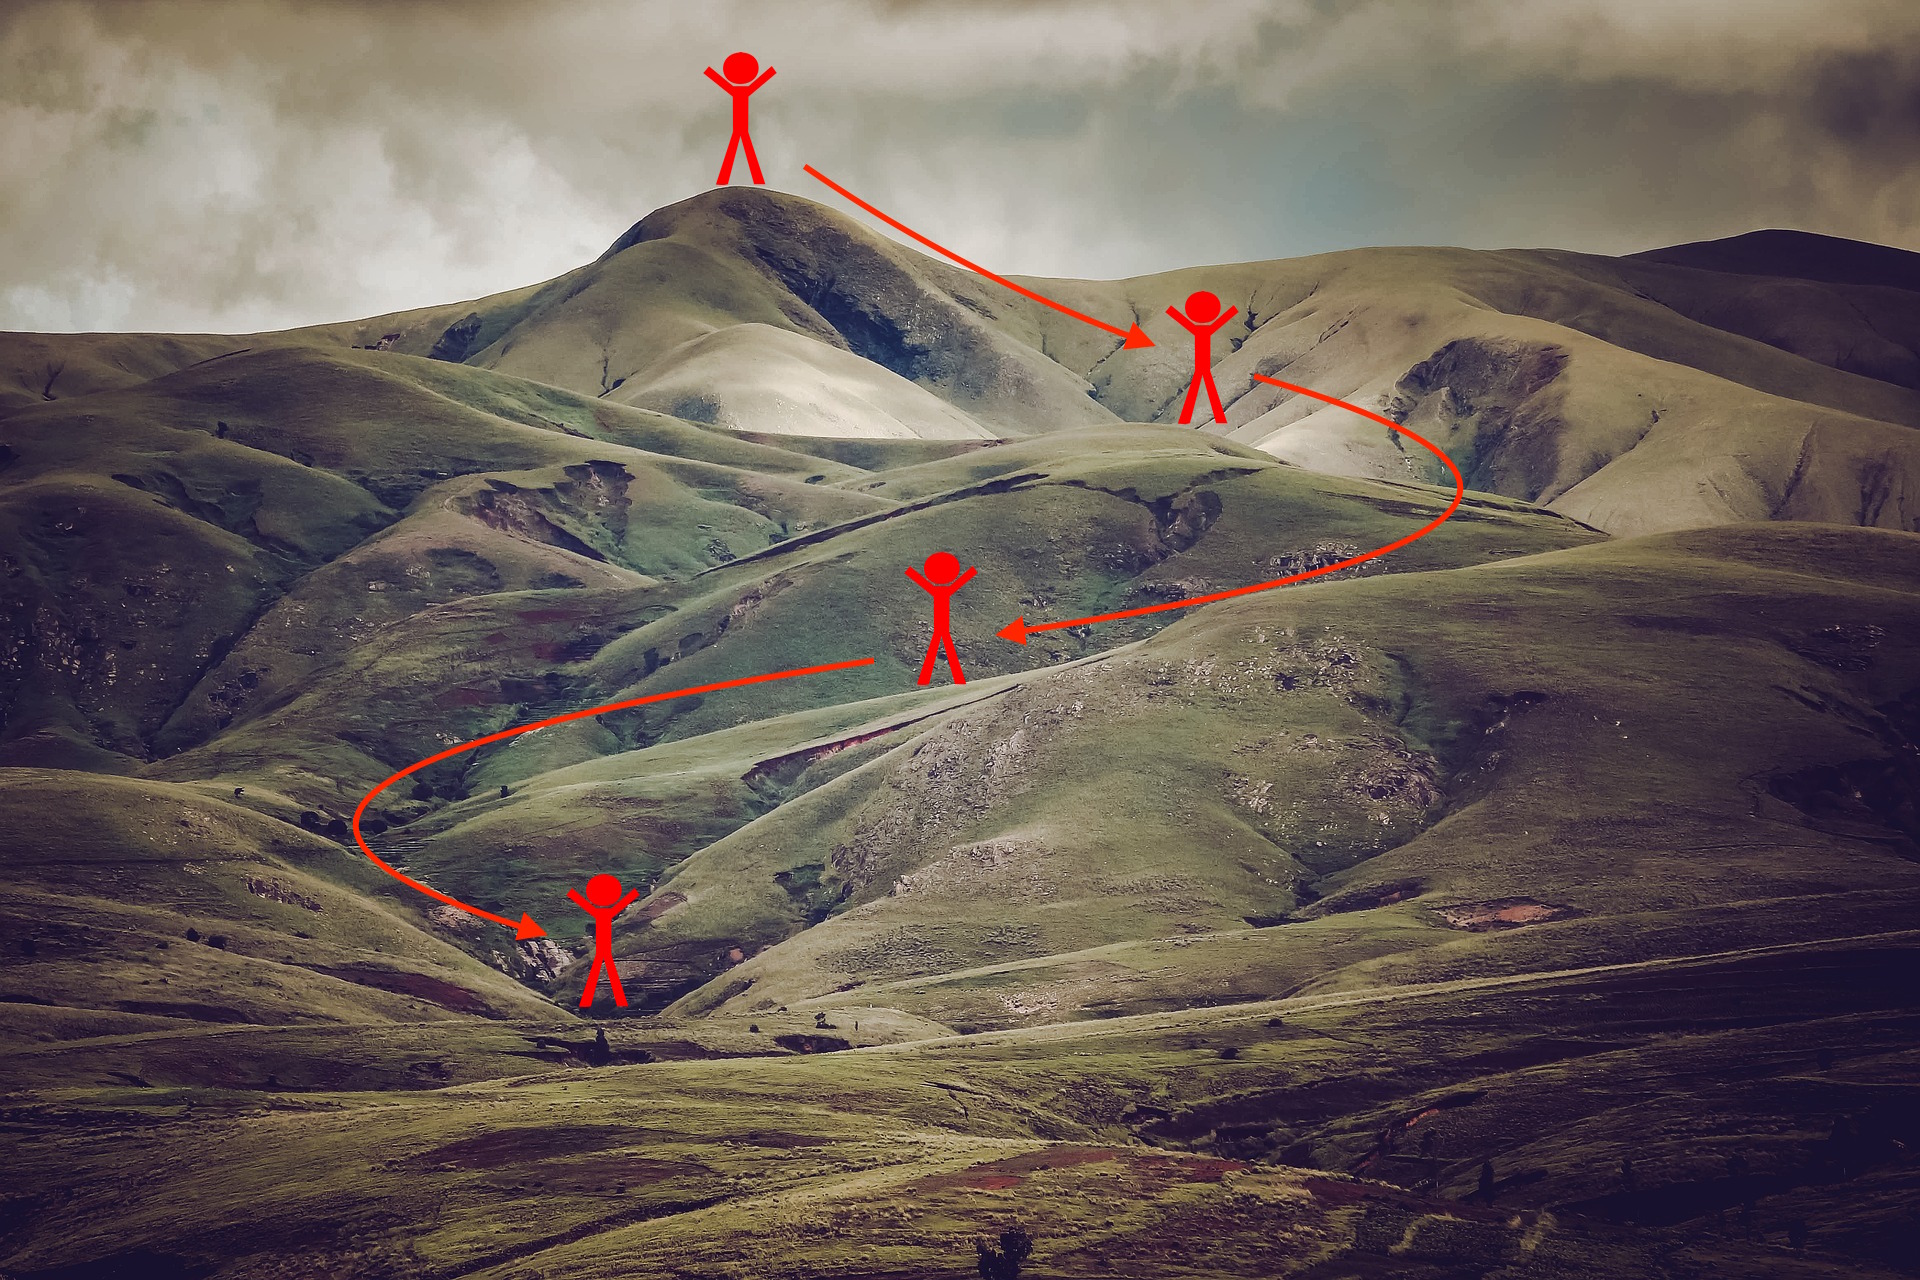
\includegraphics[width=0.7\textwidth]{course2/downhill}
\end{center}
\caption{ Minimizing the cost is like finding the lowest point in a hilly landscape}
\label{fig:downhill}
\end{figure}


By completing this assignment you will:
\begin{itemize}
\item Understand the intuition between Adam and RMS prop
\item Recognize the importance of mini-batch gradient descent
\item Learn the effects of momentum on the overall performance of your model
\end{itemize}

This assignment prepares you well for the upcoming assignment. Take your time to complete it and make sure you get the expected outputs when working through the different exercises. In some code blocks, you will find a ``\#GRADED FUNCTION: functionName" comment. Please do not modify it. After you are done, submit your work and check your results. You need to score 80\% to pass. Good luck :) !


\subsubsection{Packages}

{\textbf {Notations}}: As usual, $\frac{\partial J}{\partial a } = $ \emph{da} for any variable \emph{a}.

To get started, run the following code to import the libraries you will need.
\begin{minted}{python}
import numpy as np
import matplotlib.pyplot as plt
import scipy.io
import math
import sklearn
import sklearn.datasets

from opt_utils import load_params_and_grads, initialize_parameters, forward_propagation, backward_propagation
from opt_utils import compute_cost, predict, predict_dec, plot_decision_boundary, load_dataset
from testCases import *

#matplotlib inline
plt.rcParams['figure.figsize'] = (7.0, 4.0) # set default size of plots
plt.rcParams['image.interpolation'] = 'nearest'
plt.rcParams['image.cmap'] = 'gray'
\end{minted}



\subsubsection{Gradient Descent}

A simple optimization method in machine learning is gradient descent (GD). When you take gradient steps with respect to all $m$ examples on each step, it is also called {\textbf {Batch Gradient Descent}. 

{\textbf {Warm-up exercise}}: Implement the gradient descent update rule. The  gradient descent rule is, for $l = 1, ..., L$: 
\begin{align}
W^{[l]} &= W^{[l]} - \alpha \text{ } dW^{[l]}\\
b^{[l]} &= b^{[l]} - \alpha \text{ } db^{[l]} 
\end{align}
where L is the number of layers and $\alpha$ is the learning rate. All parameters should be stored in the \emph{parameters} dictionary. Note that the iterator \emph{l} starts at 0 in the \emph{for} loop while the first parameters are $W^{[1]}$ and $b^{[1]}$. You need to shift  \emph{l} to  \emph{l+1} when coding.


\begin{minted}{python}
# GRADED FUNCTION: update_parameters_with_gd
def update_parameters_with_gd(parameters, grads, learning_rate):
    """
    Update parameters using one step of gradient descent
    
    Arguments:
    parameters -- python dictionary containing your parameters to be updated:
                    parameters['W' + str(l)] = Wl
                    parameters['b' + str(l)] = bl
    grads -- python dictionary containing your gradients to update each parameters:
                    grads['dW' + str(l)] = dWl
                    grads['db' + str(l)] = dbl
    learning_rate -- the learning rate, scalar.
    
    Returns:
    parameters -- python dictionary containing your updated parameters 
    """

    L = len(parameters) // 2 # number of layers in the neural networks

    # Update rule for each parameter
    for l in range(L):
        ### START CODE HERE ### (approx. 2 lines)
        parameters["W" + str(l+1)] = parameters["W" + str(l+1)] - learning_rate*grads['dW' + str(l+1)]
        parameters["b" + str(l+1)] = parameters["b" + str(l+1)] - learning_rate*grads['db' + str(l+1)]
        ### END CODE HERE ###
        
    return parameters
\end{minted}

A variant of this is Stochastic Gradient Descent (SGD), which is equivalent to mini-batch gradient descent where each mini-batch has just 1 example. The update rule that you have just implemented does not change. What changes is that you would be computing gradients on just one training example at a time, rather than on the whole training set. The code examples below illustrate the difference between stochastic gradient descent and (batch) gradient descent.
\begin{tcolorbox}[title=(Batch) Gradient Descent]
\begin{minted}{python}
X = data_input
Y = labels
parameters = initialize_parameters(layers_dims)
for i in range(0, num_iterations):
    # Forward propagation
    a, caches = forward_propagation(X, parameters)
    # Compute cost.
    cost = compute_cost(a, Y)
    # Backward propagation.
    grads = backward_propagation(a, caches, parameters)
    # Update parameters.
    parameters = update_parameters(parameters, grads)
\end{minted}
\end{tcolorbox}

\clearpage
\begin{tcolorbox}[title=Stochastic Gradient Descent]
\begin{minted}{python}
X = data_input
Y = labels
parameters = initialize_parameters(layers_dims)
for i in range(0, num_iterations):
    for j in range(0, m):
        # Forward propagation
        a, caches = forward_propagation(X[:,j], parameters)
        # Compute cost
        cost = compute_cost(a, Y[:,j])
        # Backward propagation
        grads = backward_propagation(a, caches, parameters)
        # Update parameters.
        parameters = update_parameters(parameters, grads)
\end{minted}
\end{tcolorbox}

In Stochastic Gradient Descent, you use only 1 training example before updating the gradients. When the training set is large, SGD can be faster. But the parameters will ``oscillate" toward the minimum rather than converge smoothly. Here is an illustration of this:

\begin{figure}[h]
\begin{center}
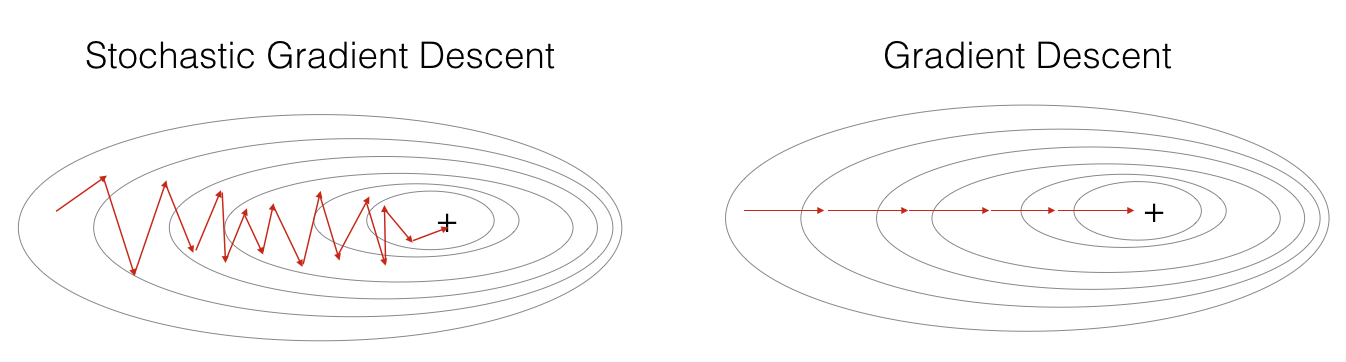
\includegraphics[width=\textwidth]{course2/SGD_vs_GD}
\end{center}
\caption{ SGD vs GD(``+" denotes a minimum of the cost. SGD leads to many oscillations to reach convergence. But each step is a lot faster to compute for SGD than for GD, as it uses only one training example (vs. the whole batch for GD).)}
\label{fig:SGD_vs_GD}
\end{figure}


{\textbf {Note}} also that implementing SGD requires 3 for-loops in total:
\begin{itemize}
\item[1.] Over the number of iterations
\item[2.] Over the $m$ training examples
\item[3.] Over the layers (to update all parameters, from $(W^{[1]},b^{[1]})$ to $(W^{[L]},b^{[L]})$)
\end{itemize}

In practice, you'll often get faster results if you do not use neither the whole training set, nor only one training example, to perform each update. Mini-batch gradient descent uses an intermediate number of examples for each step. With mini-batch gradient descent, you loop over the mini-batches instead of looping over individual training examples.
\clearpage
\begin{figure}[h]
\begin{center}
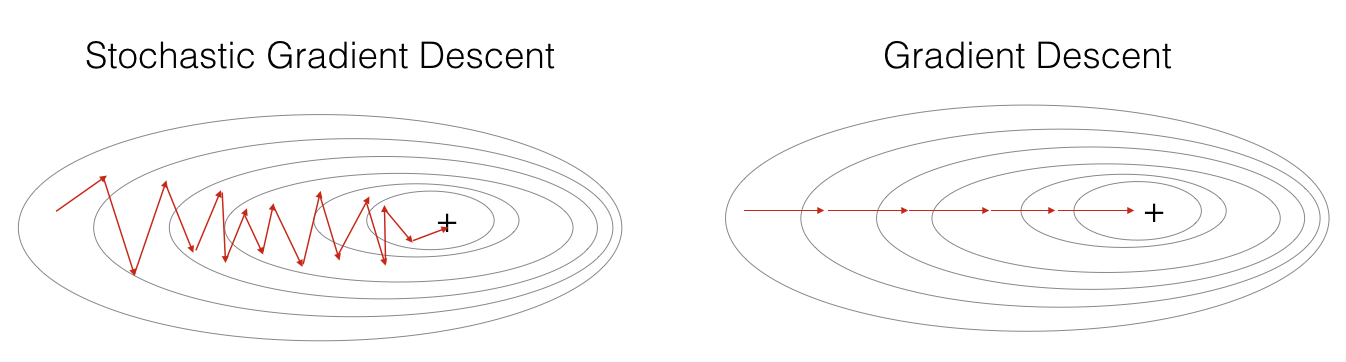
\includegraphics[width=\textwidth]{course2/SGD_vs_GD}
\end{center}
\caption{ SGD vs Mini-Batch GD(``+" denotes a minimum of the cost. Using mini-batches in your optimization algorithm often leads to faster optimization.)}
\label{fig: SGD_vs_Mini-Batch_GD}
\end{figure}



{\color{red} {\textbf {What you should remember}}:
\begin{itemize}
\item The difference between gradient descent, mini-batch gradient descent and stochastic gradient descent is the number of examples you use to perform one update step.
\item You have to tune a learning rate hyperparameter $\alpha$.
\item With a well-turned mini-batch size, usually it outperforms either gradient descent or stochastic gradient descent (particularly when the training set is large).
\end{itemize}
}



\subsubsection{Mini-Batch Gradient descent}

Let's learn how to build mini-batches from the training set (X, Y).

There are two steps:
\begin{itemize}
\item {\textbf {Shuffle}}: Create a shuffled version of the training set (X, Y) as shown below. Each column of X and Y represents a training example. Note that the random shuffling is done synchronously between X and Y. Such that after the shuffling the $i^{th}$ column of X is the example corresponding to the $i^{th}$ label in Y. The shuffling step ensures that examples will be split randomly into different mini-batches. 
\begin{figure}[h]
\begin{center}
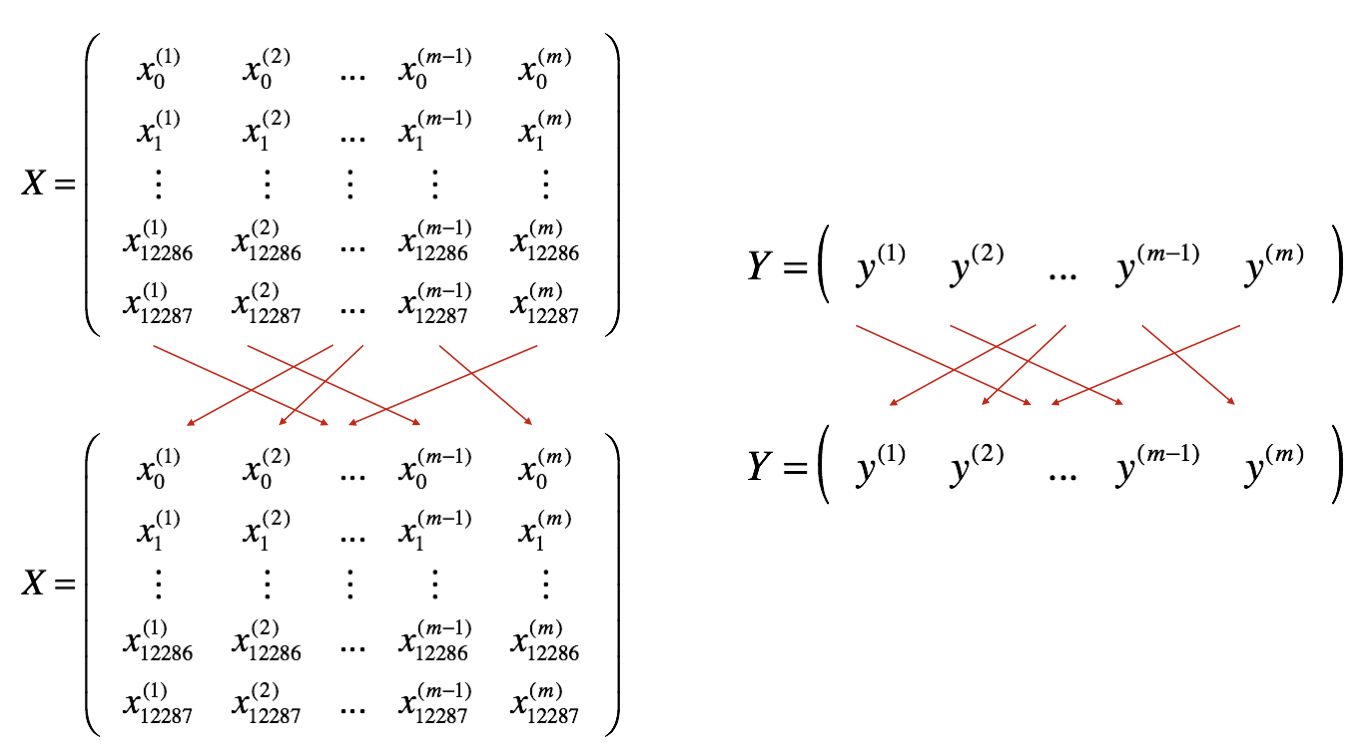
\includegraphics[width=0.8\textwidth]{course2/shuffle}
\end{center}
\caption{shuffle}
\end{figure}

\item {\textbf {Partition}}: Partition the shuffled (X, Y) into mini-batches of size \emph{mini\_batch\_size} (here 64). Note that the number of training examples is not always divisible by \emph{mini\_batch\_size}. The last mini batch might be smaller, but you don't need to worry about this. When the final mini-batch is smaller than the full \emph{mini\_batch\_size}, it will look like this: 
\begin{figure}[h]
\begin{center}
\includegraphics[width=0.8\textwidth]{course2/Partition}
\end{center}
\caption{Partition}
\end{figure}

\end{itemize}

{\textbf {Exercise}}: Implement \emph{random\_mini\_batches}. We coded the shuffling part for you. To help you with the partitioning step, we give you the following code that selects the indexes for the $1^{st}$ and $2^{nd}$ mini-batches:
\begin{minted}{python}
first_mini_batch_X = shuffled_X[:, 0 : mini_batch_size]
second_mini_batch_X = shuffled_X[:, mini_batch_size : 2 * mini_batch_size]
...
\end{minted}

Note that the last mini-batch might end up smaller than \emph{mini\_batch\_size=64}. Let $\lfloor s \rfloor$ represents $s$ rounded down to the nearest integer (this is \emph{math.floor(s)} in Python). If the total number of examples is not a multiple of \emph{mini\_batch\_size=64} then there will be $\lfloor \frac{m}{mini\_batch\_size}\rfloor$ mini-batches with a full 64 examples, and the number of examples in the final mini-batch will be ($m-mini_\_batch_\_size \times \lfloor \frac{m}{mini\_batch\_size}\rfloor$). 

\begin{minted}{python}
# GRADED FUNCTION: random_mini_batches
def random_mini_batches(X, Y, mini_batch_size = 64, seed = 0):
    """
    Creates a list of random minibatches from (X, Y)
    
    Arguments:
    X -- input data, of shape (input size, number of examples)
    Y -- true "label" vector (1 for blue dot / 0 for red dot), of shape (1, number of examples)
    mini_batch_size -- size of the mini-batches, integer
    
    Returns:
    mini_batches -- list of synchronous (mini_batch_X, mini_batch_Y)
    """
    
    np.random.seed(seed)            # To make your "random" minibatches the same as ours
    m = X.shape[1]                  # number of training examples
    mini_batches = []
        
    # Step 1: Shuffle (X, Y)
    permutation = list(np.random.permutation(m))
    shuffled_X = X[:, permutation]
    shuffled_Y = Y[:, permutation].reshape((1,m))

    # Step 2: Partition (shuffled_X, shuffled_Y). Minus the end case.
    num_complete_minibatches = math.floor(m/mini_batch_size) # number of mini batches of size mini_batch_size in your partitionning
    for k in range(0, num_complete_minibatches):
        ### START CODE HERE ### (approx. 2 lines)
        mini_batch_X = shuffled_X[:, mini_batch_size*k: mini_batch_size*(k+1)]
        mini_batch_Y = shuffled_Y[:, mini_batch_size*k: mini_batch_size*(k+1)]
        ### END CODE HERE ###
        mini_batch = (mini_batch_X, mini_batch_Y)
        mini_batches.append(mini_batch)
    
    # Handling the end case (last mini-batch < mini_batch_size)
    if m % mini_batch_size != 0:
        ### START CODE HERE ### (approx. 2 lines)
        mini_batch_X = shuffled_X[:,num_complete_minibatches * mini_batch_size : m]
        mini_batch_Y = shuffled_Y[:,num_complete_minibatches * mini_batch_size : m]
        ### END CODE HERE ###
        mini_batch = (mini_batch_X, mini_batch_Y)
        mini_batches.append(mini_batch)
    
    return mini_batches
\end{minted}

{\color{red}\textbf{What you should remember:}
\begin{itemize}
\item Shuffling and Partitioning are the two steps required to build mini-batches
\item Powers of two are often chosen to be the mini-batch size, e.g., 16, 32, 64, 128.
\end{itemize}
}



\subsubsection{Momentum}

Because mini-batch gradient descent makes a parameter update after seeing just a subset of examples, the direction of the update has some variance, and so the path taken by mini-batch gradient descent will ``oscillate" toward convergence. Using momentum can reduce these oscillations.


Momentum takes into account the past gradients to smooth out the update. We will store the \emph{direction} of the previous gradients in the variable  $v$ . Formally, this will be the exponentially weighted average of the gradient on previous steps. You can also think of  $v$  as the ``velocity" of a ball rolling downhill, building up speed (and momentum) according to the direction of the gradient/slope of the hill.
\begin{figure}[h]
\begin{center}
\includegraphics[width=0.8\textwidth]{course2/Momentum}
\end{center}
\caption{The {\color{red}red arrows} shows the direction taken by one step of mini-batch gradient descent with momentum. The {\color{blue}blue points} show the direction of the gradient (with respect to the current mini-batch) on each step. Rather than just following the gradient, we let the gradient influence  $v$ and then take a step in the direction of $v$}
\end{figure}


{\textbf{Exercise}}: Initialize the velocity. The velocity, $v$, is a python dictionary that needs to be initialized with arrays of zeros. Its keys are the same as those in the \emph{grads} dictionary, that is: for $l =1,...,L$:
\begin{minted}{python}
v["dW" + str(l+1)] = ... #(numpy array of zeros with the same shape as parameters["W" + str(l+1)])
v["db" + str(l+1)] = ... #(numpy array of zeros with the same shape as parameters["b" + str(l+1)])
\end{minted}

{\textbf{Note}} that the iterator l starts at 0 in the for loop while the first parameters are v[``dW1"] and v[``db1"] (that's a ``one" on the superscript). This is why we are shifting l to l+1 in the \emph{for} loop.


\begin{minted}{python}
# GRADED FUNCTION: initialize_velocity
def initialize_velocity(parameters):
    """
    Initializes the velocity as a python dictionary with:
                - keys: "dW1", "db1", ..., "dWL", "dbL" 
                - values: numpy arrays of zeros of the same shape as the corresponding gradients/parameters.
    Arguments:
    parameters -- python dictionary containing your parameters.
                    parameters['W' + str(l)] = Wl
                    parameters['b' + str(l)] = bl
    
    Returns:
    v -- python dictionary containing the current velocity.
                    v['dW' + str(l)] = velocity of dWl
                    v['db' + str(l)] = velocity of dbl
    """
    
    L = len(parameters) // 2 # number of layers in the neural networks
    v = {}
    
    # Initialize velocity
    for l in range(L):
        ### START CODE HERE ### (approx. 2 lines)
        v["dW" + str(l+1)] = np.zeros(parameters['W' + str(l+1)].shape)
        v["db" + str(l+1)] = np.zeros(parameters['b' + str(l+1)].shape)
        ### END CODE HERE ###
        
    return v
\end{minted}


{\textbf{Exercise}}:  Now, implement the parameters update with momentum. The momentum update rule is, for $l = 1, ..., L$: 
\begin{align}
\begin{cases}
v_{dW^{[l]}} = \beta v_{dW^{[l]}} + (1 - \beta) dW^{[l]} \\
W^{[l]} = W^{[l]} - \alpha v_{dW^{[l]}}
\end{cases}
\end{align}
\begin{align}
\begin{cases}
v_{db^{[l]}} = \beta v_{db^{[l]}} + (1 - \beta) db^{[l]} \\
b^{[l]} = b^{[l]} - \alpha v_{db^{[l]}} 
\end{cases}
\end{align}
where L is the number of layers, $\beta$ is the momentum and $\alpha$ is the learning rate. All parameters should be stored in the \emph{parameters} dictionary.  Note that the iterator \emph{l} starts at 0 in the \emph{for} loop while the first parameters are $W^{[1]}$ and $b^{[1]}$ (that's a ``one" on the superscript). So you will need to shift \emph{l} to \emph{l+1} when coding.

\begin{minted}{python}
# GRADED FUNCTION: update_parameters_with_momentum
def update_parameters_with_momentum(parameters, grads, v, beta, learning_rate):
    """
    Update parameters using Momentum
    
    Arguments:
    parameters -- python dictionary containing your parameters:
                    parameters['W' + str(l)] = Wl
                    parameters['b' + str(l)] = bl
    grads -- python dictionary containing your gradients for each parameters:
                    grads['dW' + str(l)] = dWl
                    grads['db' + str(l)] = dbl
    v -- python dictionary containing the current velocity:
                    v['dW' + str(l)] = ...
                    v['db' + str(l)] = ...
    beta -- the momentum hyperparameter, scalar
    learning_rate -- the learning rate, scalar
    
    Returns:
    parameters -- python dictionary containing your updated parameters 
    v -- python dictionary containing your updated velocities
    """

    L = len(parameters) // 2 # number of layers in the neural networks
    
    # Momentum update for each parameter
    for l in range(L):
        
        ### START CODE HERE ### (approx. 4 lines)
        # compute velocities
        v["dW" + str(l+1)] = beta *  v["dW" + str(l+1)] +(1- beta )* grads['dW' + str(l+1)]
        v["db" + str(l+1)] = beta *  v["db" + str(l+1)] +(1- beta )* grads['db' + str(l+1)]
        # update parameters
        parameters["W" + str(l+1)] = parameters["W" + str(l+1)]- learning_rate * v["dW" + str(l+1)]
        parameters["b" + str(l+1)] = parameters["b" + str(l+1)]- learning_rate * v["db" + str(l+1)]
        ### END CODE HERE ###
        
    return parameters, v
\end{minted}

{\textbf{Note}} that:
\begin{itemize}
\item The velocity is initialized with zeros. So the algorithm will take a few iterations to ``build up" velocity and start to take bigger steps.
\item If $\beta = 0$, then this just becomes standard gradient descent without momentum. 
\end{itemize}

{\textbf{How do you choose $\beta$?}}
\begin{itemize}
\item The larger the momentum $\beta$ is, the smoother the update because the more we take the past gradients into account. But if $\beta$ is too big, it could also smooth out the updates too much. 
\item Common values for $\beta$ range from 0.8 to 0.999. If you don't feel inclined to tune this, $\beta = 0.9$ is often a reasonable default. 
\item Tuning the optimal $\beta$ for your model might need trying several values to see what works best in term of reducing the value of the cost function $J$. 
\end{itemize}

{\color{red}\textbf{What you should remember}:
\begin{itemize}
\item Momentum takes past gradients into account to smooth out the steps of gradient descent. It can be applied with batch gradient descent, mini-batch gradient descent or stochastic gradient descent.
\item You have to tune a momentum hyperparameter $\beta$ and a learning rate $\alpha$.
\end{itemize}
}



\subsubsection{Adam}

Adam is one of the most effective optimization algorithms for training neural networks. It combines ideas from RMSProp (described in lecture) and Momentum. 

{\textbf{How does Adam work?}}
\begin{itemize}
\item[1.] It calculates an exponentially weighted average of past gradients, and stores it in variables $v$ (before bias correction) and $v^{corrected}$ (with bias correction). 
\item[2.] It calculates an exponentially weighted average of the squares of the past gradients, and  stores it in variables $s$ (before bias correction) and $s^{corrected}$ (with bias correction). 
\item[3.] It updates parameters in a direction based on combining information from ``1" and ``2".
\end{itemize}
The update rule is, for $l = 1, ..., L$: 
\begin{align}
\begin{cases}
v_{dW^{[l]}} = \beta_1 v_{dW^{[l]}} + (1 - \beta_1) \frac{\partial \mathcal{J} }{ \partial W^{[l]} } \\
v^{corrected}_{dW^{[l]}} = \frac{v_{dW^{[l]}}}{1 - (\beta_1)^t} \\
s_{dW^{[l]}} = \beta_2 s_{dW^{[l]}} + (1 - \beta_2) (\frac{\partial \mathcal{J} }{\partial W^{[l]} })^2 \\
s^{corrected}_{dW^{[l]}} = \frac{s_{dW^{[l]}}}{1 - (\beta_1)^t} \\
W^{[l]} = W^{[l]} - \alpha \frac{v^{corrected}_{dW^{[l]}}}{\sqrt{s^{corrected}_{dW^{[l]}}} + \varepsilon}
\end{cases}
\end{align}
where:
\begin{itemize}
\item t counts the number of steps taken of Adam 
\item L is the number of layers
\item $\beta_1$ and $\beta_2$ are hyperparameters that control the two exponentially weighted averages. 
\item $\alpha$ is the learning rate
\item $\varepsilon$ is a very small number to avoid dividing by zero
\end{itemize}

As usual, we will store all parameters in the \emph{parameters} dictionary  


{\textbf{Exercise}}: Initialize the Adam variables $v, s$ which keep track of the past information.

{\textbf{Instruction}}: The variables $v, s$ are python dictionaries that need to be initialized with arrays of zeros. Their keys are the same as for \emph{grads}, that is: for $l = 1, ..., L$:
\begin{minted}{python}
v["dW" + str(l+1)] = ... #(numpy array of zeros with the same shape as parameters["W" + str(l+1)])
v["db" + str(l+1)] = ... #(numpy array of zeros with the same shape as parameters["b" + str(l+1)])
s["dW" + str(l+1)] = ... #(numpy array of zeros with the same shape as parameters["W" + str(l+1)])
s["db" + str(l+1)] = ... #(numpy array of zeros with the same shape as parameters["b" + str(l+1)])
\end{minted}


\begin{minted}{python}
# GRADED FUNCTION: initialize_adam
def initialize_adam(parameters) :
    """
    Initializes v and s as two python dictionaries with:
                - keys: "dW1", "db1", ..., "dWL", "dbL" 
                - values: numpy arrays of zeros of the same shape as the corresponding gradients/parameters.
    
    Arguments:
    parameters -- python dictionary containing your parameters.
                    parameters["W" + str(l)] = Wl
                    parameters["b" + str(l)] = bl
    
    Returns: 
    v -- python dictionary that will contain the exponentially weighted average of the gradient.
                    v["dW" + str(l)] = ...
                    v["db" + str(l)] = ...
    s -- python dictionary that will contain the exponentially weighted average of the squared gradient.
                    s["dW" + str(l)] = ...
                    s["db" + str(l)] = ...

    """
    
    L = len(parameters) // 2 # number of layers in the neural networks
    v = {}
    s = {}
    
    # Initialize v, s. Input: "parameters". Outputs: "v, s".
    for l in range(L):
    ### START CODE HERE ### (approx. 4 lines)
        v["dW" + str(l+1)] = np.zeros(parameters["W" + str(l+1)].shape)
        v["db" + str(l+1)] = np.zeros(parameters["b" + str(l+1)].shape)
        s["dW" + str(l+1)] = np.zeros(parameters["W" + str(l+1)].shape)
        s["db" + str(l+1)] = np.zeros(parameters["b" + str(l+1)].shape)
    ### END CODE HERE ###
    
    return v, s
\end{minted}




{\textbf{Exercise}}:  Now, implement the parameters update with Adam. Recall the general update rule is, for $l = 1, ..., L$: 
\begin{align*}
\begin{cases}
v_{W^{[l]}} = \beta_1 v_{W^{[l]}} + (1 - \beta_1) \frac{\partial J }{ \partial W^{[l]} } \\
v^{corrected}_{W^{[l]}} = \frac{v_{W^{[l]}}}{1 - (\beta_1)^t} \\
s_{W^{[l]}} = \beta_2 s_{W^{[l]}} + (1 - \beta_2) (\frac{\partial J }{\partial W^{[l]} })^2 \\
s^{corrected}_{W^{[l]}} = \frac{s_{W^{[l]}}}{1 - (\beta_2)^t} \\
W^{[l]} = W^{[l]} - \alpha \frac{v^{corrected}_{W^{[l]}}}{\sqrt{s^{corrected}_{W^{[l]}}}+\varepsilon}
\end{cases}
\end{align*}

{\textbf{Note}} that the iterator \emph{l} starts at 0 in the \emph{for} loop while the first parameters are $W^{[1]}$ and $b^{[1]}$. You need to shift \emph{l} to \emph{l+1} when coding.

\begin{minted}{python}
# GRADED FUNCTION: update_parameters_with_adam
def update_parameters_with_adam(parameters, grads, v, s, t, learning_rate = 0.01, beta1 = 0.9, beta2 = 0.999,  epsilon = 1e-8):
    """
    Update parameters using Adam
    
    Arguments:
    parameters -- python dictionary containing your parameters:
                    parameters['W' + str(l)] = Wl
                    parameters['b' + str(l)] = bl
    grads -- python dictionary containing your gradients for each parameters:
                    grads['dW' + str(l)] = dWl
                    grads['db' + str(l)] = dbl
    v -- Adam variable, moving average of the first gradient, python dictionary
    s -- Adam variable, moving average of the squared gradient, python dictionary
    learning_rate -- the learning rate, scalar.
    beta1 -- Exponential decay hyperparameter for the first moment estimates 
    beta2 -- Exponential decay hyperparameter for the second moment estimates 
    epsilon -- hyperparameter preventing division by zero in Adam updates

    Returns:
    parameters -- python dictionary containing your updated parameters 
    v -- Adam variable, moving average of the first gradient, python dictionary
    s -- Adam variable, moving average of the squared gradient, python dictionary
    """
    
    L = len(parameters) // 2  # number of layers in the neural networks
    v_corrected = {}    # Initializing first moment estimate, python dictionary
    s_corrected = {}    # Initializing second moment estimate, python dictionary
    
    # Perform Adam update on all parameters
    for l in range(L):
        # Moving average of the gradients. Inputs: "v, grads, beta1". Output: "v".
        v["dW" + str(l+1)] = beta1*v["dW" + str(l+1)]+(1-beta1)*grads['dW' + str(l+1)]
        v["db" + str(l+1)] = beta1*v["db" + str(l+1)]+(1-beta1)*grads['db' + str(l+1)]

        # Compute bias-corrected first moment estimate. Inputs: "v, beta1, t". Output: "v_corrected".
        v_corrected["dW" + str(l+1)] = v["dW" + str(l+1)]/(1-math.pow(beta1,t))
        v_corrected["db" + str(l+1)] = v["db" + str(l+1)]/(1-math.pow(beta1,t))

        # Moving average of the squared gradients. Inputs: "s, grads, beta2". Output: "s".
        s["dW" + str(l+1)] = beta2*s["dW" + str(l+1)]+(1-beta2)*(grads['dW' + str(l+1)]**2)
        s["db" + str(l+1)] = beta2*s["db" + str(l+1)]+(1-beta2)*(grads['db' + str(l+1)]**2)

        # Compute bias-corrected second raw moment estimate. Inputs: "s, beta2, t". Output: "s_corrected".
        s_corrected["dW" + str(l+1)] = s["dW" + str(l+1)]/(1-math.pow(beta2,t))
        s_corrected["db" + str(l+1)] = s["db" + str(l+1)]/(1-math.pow(beta2,t))

        # Update parameters. Inputs: "parameters, learning_rate, v_corrected, s_corrected, epsilon". Output: "parameters".
        parameters["W" + str(l+1)] = parameters["W" + str(l+1)]-learning_rate * v_corrected["dW" + str(l+1)]/(np.sqrt(s_corrected["dW" + str(l+1)])+epsilon)
        parameters["b" + str(l+1)] = parameters["b" + str(l+1)]-learning_rate * v_corrected["db" + str(l+1)]/(np.sqrt(s_corrected["db" + str(l+1)])+epsilon)

    return parameters, v, s
\end{minted}

You now have three working optimization algorithms (mini-batch gradient descent, Momentum, Adam). Let's implement a model with each of these optimizers and observe the difference.



\subsubsection{Model with different optimization algorithms}
Lets use the following ``moons" dataset to test the different optimization methods. (The dataset is named ``moons" because the data from each of the two classes looks a bit like a crescent-shaped moon.)
\begin{minted}{python}
train_X, train_Y = load_dataset()
\end{minted}

\begin{figure}[h]
\begin{center}
\includegraphics[width=0.8\textwidth]{course2/moons_data}
\end{center}
\end{figure}


We have already implemented a 3-layer neural network. You will train it with:
\begin{itemize} 
\item Mini-batch {\textbf{Gradient Descent}}: it will call your function:
    \begin{itemize} 
    \item update\_parameters\_with\_gd()
    \end{itemize} 
\item Mini-batch {\textbf {Momentum}}: it will call your functions:
      \begin{itemize} 
      \item initialize\_velocity() and update\_parameters\_with\_momentum()
      \end{itemize} 
\item Mini-batch {\textbf{Adam}}: it will call your functions:
      \begin{itemize} 
     \item initialize\_adam() and update\_parameters\_with\_adam()
      \end{itemize} 
\end{itemize} 

\begin{minted}{python}
def model(X, Y, layers_dims, optimizer, learning_rate = 0.0007, mini_batch_size = 64, beta = 0.9, beta1 = 0.9, beta2 = 0.999,  epsilon = 1e-8, num_epochs = 10000, print_cost = True):
    """
    3-layer neural network model which can be run in different optimizer modes.
    
    Arguments:
    X -- input data, of shape (2, number of examples)
    Y -- true "label" vector (1 for blue dot / 0 for red dot), of shape (1, number of examples)
    layers_dims -- python list, containing the size of each layer
    learning_rate -- the learning rate, scalar.
    mini_batch_size -- the size of a mini batch
    beta -- Momentum hyperparameter
    beta1 -- Exponential decay hyperparameter for the past gradients estimates 
    beta2 -- Exponential decay hyperparameter for the past squared gradients estimates 
    epsilon -- hyperparameter preventing division by zero in Adam updates
    num_epochs -- number of epochs
    print_cost -- True to print the cost every 1000 epochs

    Returns:
    parameters -- python dictionary containing your updated parameters 
    """

    L = len(layers_dims) # number of layers in the neural networks
    costs = []   # to keep track of the cost
    t = 0       # initializing the counter required for Adam update
    seed = 10   # For grading purposes, so that your "random" minibatches are the same as ours
    
    # Initialize parameters
    parameters = initialize_parameters(layers_dims)

    # Initialize the optimizer
    if optimizer == "gd":
        pass # no initialization required for gradient descent
    elif optimizer == "momentum":
        v = initialize_velocity(parameters)
    elif optimizer == "adam":
        v, s = initialize_adam(parameters)
    
    # Optimization loop
    for i in range(num_epochs):
        
        # Define the random minibatches. We increment the seed to reshuffle differently the dataset after each epoch
        seed = seed + 1
        minibatches = random_mini_batches(X, Y, mini_batch_size, seed)

        for minibatch in minibatches:

            # Select a minibatch
            (minibatch_X, minibatch_Y) = minibatch

            # Forward propagation
            a3, caches = forward_propagation(minibatch_X, parameters)

            # Compute cost
            cost = compute_cost(a3, minibatch_Y)

            # Backward propagation
            grads = backward_propagation(minibatch_X, minibatch_Y, caches)

            # Update parameters
            if optimizer == "gd":
                parameters = update_parameters_with_gd(parameters, grads, learning_rate)
            elif optimizer == "momentum":
                parameters, v = update_parameters_with_momentum(parameters, grads, v, beta, learning_rate)
            elif optimizer == "adam":
                t = t + 1 # Adam counter
                parameters, v, s = update_parameters_with_adam(parameters, grads, v, s, t, learning_rate, beta1, beta2,  epsilon)
        
        # Print the cost every 1000 epoch
        if print_cost and i % 1000 == 0:
            print ("Cost after epoch %i: %f" %(i, cost))
        if print_cost and i % 100 == 0:
            costs.append(cost)
                
    # plot the cost
    plt.plot(costs)
    plt.ylabel('cost')
    plt.xlabel('epochs (per 100)')
    plt.title("Learning rate = " + str(learning_rate))
    plt.show()

    return parameters
\end{minted}


You will now run this 3 layer neural network with each of the 3 optimization methods.

\clearpage
\subsubsubsection{Mini-batch Gradient descent}

Run the following code to see how the model does with mini-batch gradient descent.
\begin{minted}{python}
# train 3-layer model
layers_dims = [train_X.shape[0], 5, 2, 1]
parameters = model(train_X, train_Y, layers_dims, optimizer = "gd")

# Predict
predictions = predict(train_X, train_Y, parameters)

# Plot decision boundary
plt.title("Model with Gradient Descent optimization")
axes = plt.gca()
axes.set_xlim([-1.5,2.5])
axes.set_ylim([-1,1.5])
plot_decision_boundary(lambda x: predict_dec(parameters, x.T), train_X, train_Y)
\end{minted}

\begin{minted}{python}
#output
Cost after epoch 0: 0.690736
Cost after epoch 1000: 0.685273
Cost after epoch 2000: 0.647072
Cost after epoch 3000: 0.619525
Cost after epoch 4000: 0.576584
Cost after epoch 5000: 0.607243
Cost after epoch 6000: 0.529403
Cost after epoch 7000: 0.460768
Cost after epoch 8000: 0.465586
Cost after epoch 9000: 0.464518
\end{minted}

\begin{figure}[h]
\begin{center}
\includegraphics[width=0.8\textwidth]{course2/gd_cost}
\end{center}
\end{figure}

\begin{figure}[h]
\begin{center}
\includegraphics[width=0.8\textwidth]{course2/gd_result}
\caption{Model with Gradient Descent optimization}
\end{center}
\end{figure}


\subsubsubsection{Mini-batch gradient descent with momentum}
\begin{minted}{python}
# train 3-layer model
layers_dims = [train_X.shape[0], 5, 2, 1]
parameters = model(train_X, train_Y, layers_dims, beta = 0.9, optimizer = "momentum")

# Predict
predictions = predict(train_X, train_Y, parameters)

# Plot decision boundary
plt.title("Model with Momentum optimization")
axes = plt.gca()
axes.set_xlim([-1.5,2.5])
axes.set_ylim([-1,1.5])
plot_decision_boundary(lambda x: predict_dec(parameters, x.T), train_X, train_Y)
\end{minted}


\begin{minted}{python}
#output
Cost after epoch 0: 0.690741
Cost after epoch 1000: 0.685341
Cost after epoch 2000: 0.647145
Cost after epoch 3000: 0.619594
Cost after epoch 4000: 0.576665
Cost after epoch 5000: 0.607324
Cost after epoch 6000: 0.529476
Cost after epoch 7000: 0.460936
Cost after epoch 8000: 0.465780
Cost after epoch 9000: 0.464740
\end{minted}

\begin{figure}[h]
\begin{center}
\includegraphics[width=0.8\textwidth]{course2/Momentum_cost}
\end{center}
\end{figure}

\begin{figure}[h]
\begin{center}
\includegraphics[width=0.8\textwidth]{course2/Momentum_result}
\caption{Model with Momentum optimization}
\end{center}
\end{figure}


\subsubsubsection{Mini-batch with Adam mode}
\begin{minted}{python}
# train 3-layer model
layers_dims = [train_X.shape[0], 5, 2, 1]
parameters = model(train_X, train_Y, layers_dims, optimizer = "adam")

# Predict
predictions = predict(train_X, train_Y, parameters)

# Plot decision boundary
plt.title("Model with Adam optimization")
axes = plt.gca()
axes.set_xlim([-1.5,2.5])
axes.set_ylim([-1,1.5])
plot_decision_boundary(lambda x: predict_dec(parameters, x.T), train_X, train_Y)
\end{minted}

\begin{minted}{python}
#output
Cost after epoch 0: 0.690552
Cost after epoch 1000: 0.185567
Cost after epoch 2000: 0.150852
Cost after epoch 3000: 0.074454
Cost after epoch 4000: 0.125936
Cost after epoch 5000: 0.104235
Cost after epoch 6000: 0.100552
Cost after epoch 7000: 0.031601
Cost after epoch 8000: 0.111709
Cost after epoch 9000: 0.197648
\end{minted}

\begin{figure}[h]
\begin{center}
\includegraphics[width=0.8\textwidth]{course2/Adam_cost}
\end{center}
\end{figure}

\clearpage
\begin{figure}[h]
\begin{center}
\includegraphics[width=0.8\textwidth]{course2/Adam_result}
\caption{Model with Adam optimization}
\end{center}
\end{figure}



\subsubsubsection{Summary}
\begin{table}[h]
\centering
\begin{tabular}{ccc}
\toprule
optimization method	&accuracy	&cost shape\\
\midrule
Gradient descent	&79.7\%&	oscillations\\
Momentum	&79.7\%	& oscillations\\
Adam	&94\%	&smoother\\
\bottomrule
\end{tabular}
\end{table}


Momentum usually helps, but given the small learning rate and the simplistic dataset, its impact is almost negligeable. Also, the huge oscillations you see in the cost come from the fact that some minibatches are more difficult thans others for the optimization algorithm.

Adam on the other hand, clearly outperforms mini-batch gradient descent and Momentum. If you run the model for more epochs on this simple dataset, all three methods will lead to very good results. However, you've seen that Adam converges a lot faster.

Some advantages of Adam include:
\begin{itemize}
\item Relatively low memory requirements (though higher than gradient descent and gradient descent with momentum) 
\item Usually works well even with little tuning of hyperparameters (except $\alpha$)
\end{itemize}
\clearpage
\subsection{Tensorflow}

Welcome to the Tensorflow Tutorial! Until now, you've always used numpy to build neural networks. Now we will step you through a deep learning framework that will allow you to build neural networks more easily. Machine learning frameworks like TensorFlow, PaddlePaddle, Torch, Caffe, Keras, and many others can speed up your machine learning development significantly. All of these frameworks also have a lot of documentation, which you should feel free to read. In this programming assignment you will learn all the basics of Tensorflow. You will implement useful functions and draw the parallel with what you did using Numpy. You will understand what Tensors and operations are, as well as how to execute them in a computation graph.

In this assignment, you will learn to do the following in TensorFlow:
\begin{itemize}
\item Initialize variables
\item Start your own session
\item Train algorithms
\item Implement a Neural Network
\end{itemize}

Programing frameworks can not only shorten your coding time, but sometimes also perform optimizations that speed up your code.


After completing this assignment you will also be able to implement your own deep learning models using Tensorflow. In fact, using our brand new SIGNS dataset, you will build a deep neural network model to recognize numbers from 0 to 5 in sign language with a pretty impressive accuracy.

\begin{figure}[h]
\begin{center}
\includegraphics[width=\textwidth]{course2/recognize_numbers}
\end{center}
\label{fig:recognize_numbers}
\end{figure}



\subsubsection{Exploring the Tensorflow Library}
To start, you will import the library:

\begin{minted}{python}
import math
import numpy as np
import h5py
import matplotlib.pyplot as plt
import tensorflow as tf
from tensorflow.python.framework import ops
from tf_utils import load_dataset, random_mini_batches, convert_to_one_hot, predict

#matplotlib inline
np.random.seed(1)
\end{minted}

Now that you have imported the library, we will walk you through its different applications. You will start with an example, where we compute for you the loss of one training example. 
\begin{align}
loss = \mathcal{L}(\hat{y}, y) = (\hat y^{(i)} - y^{(i)})^2
\end{align}


\begin{minted}{python}
# Define y_hat constant. Set to 36.
y_hat = tf.constant(36, name='y_hat')  

# Define y. Set to 39          
y = tf.constant(39, name='y') 
                   
# Create a variable for the loss
loss = tf.Variable((y - y_hat)**2, name='loss')  

# When init is run later (session.run(init))
init = tf.global_variables_initializer()         

# the loss variable will be initialized and ready to be computed
with tf.Session() as session: # Create a session and print the output
    session.run(init)         # Initializes the variables
    print(session.run(loss))  # Prints the loss
\end{minted}

Writing and running programs in TensorFlow has the following steps:
\begin{itemize}
\item[1] Create Tensors (variables) that are not yet executed/evaluated.
\item[2] Write operations between those Tensors.
\item[3] Initialize your Tensors.
\item[4] Create a Session.
\item[5] Run the Session. This will run the operations you'd written above.
\end{itemize}

Therefore, when we created a variable for the loss, we simply defined the loss as a function of other quantities, but did not evaluate its value. To evaluate it, we had to run init=tf.global\_variables\_initializer(). That initialized the loss variable, and in the last line we were finally able to evaluate the value of loss and print its value.

Now let us look at an easy example. Run the cell below:
\begin{minted}{python}
a = tf.constant(2)
b = tf.constant(10)
c = tf.multiply(a,b)
print(c)

#output
Tensor("Mul_0:0", shape=(), dtype=int32)
\end{minted}

As expected, you will not see 20! You got a tensor saying that the result is a tensor that does not have the shape attribute, and is of type ``int32". All {\textbf {you did was put in the \emph{computation graph}, but you have not run this computation yet}}. In order to actually multiply the two numbers, {\textbf {you will have to create a session and run it}}.
\begin{minted}{python}
sess = tf.Session()
print(sess.run(c))

#output
20
\end{minted}


Great! To summarize, remember to {\color{red}\textbf {initialize your variables, create a session and run the operations inside the session}}.

Next, you'll also have to know about {\textbf {placeholders}}. A placeholder is an object whose value you can specify only later. To specify values for a placeholder, you can pass in values by using a ``feed dictionary" (feed\_dict variable). Below, we created a placeholder for x. This allows us to pass in a number later when we run the session.


\begin{minted}{python}
# Change the value of x in the feed_dict

x = tf.placeholder(tf.int64, name = 'x')
print(sess.run(2 * x, feed_dict = {x: 3}))
sess.close()

#output
6
\end{minted}

When you first defined x you did not have to specify a value for it. A placeholder is simply a variable that you will assign data to only later, when running the session. We say that you {\textbf {feed data}} to these placeholders when running the session.

Here's what's happening: When you specify the operations needed for a computation, you are telling TensorFlow how to construct a computation graph. The computation graph can have some placeholders whose values you will specify only later. Finally, when you run the session, you are telling TensorFlow to execute the computation graph.


\subsubsubsection{Linear function}


Lets start this programming exercise by computing the following equation: $Y = WX + b$, where $W$ and $X$ are random matrices and b is a random vector. 

{\textbf {Exercise}}: Compute $WX + b$ where $W, X$, and $b$ are drawn from a random normal distribution. W is of shape (4, 3), X is (3,1) and b is (4,1). As an example, here is how you would define a constant X that has shape (3,1):
\begin{minted}{python}
X = tf.constant(np.random.randn(3,1), name = "X")
\end{minted}

You might find the following functions helpful: 
\begin{itemize}
\item tf.matmul(..., ...) to do a matrix multiplication
\item tf.add(..., ...) to do an addition
\item np.random.randn(...) to initialize randomly
\end{itemize}

\begin{minted}{python}
# GRADED FUNCTION: linear_function
def linear_function():
    """
    Implements a linear function: 
            Initializes W to be a random tensor of shape (4,3)
            Initializes X to be a random tensor of shape (3,1)
            Initializes b to be a random tensor of shape (4,1)
    Returns: 
    result -- runs the session for Y = WX + b 
    """
    
    np.random.seed(1)
    
    ### START CODE HERE ### (4 lines of code)
    X = tf.constant(np.random.randn(3,1), name = "X")
    W = tf.constant(np.random.randn(4,3), name = "W")
    b = tf.constant(np.random.randn(4,1), name = "b")
    Y = tf.add(tf.matmul(W,X),b)
    ### END CODE HERE ### 
    
    # Create the session using tf.Session() and run it with sess.run(...) on the variable you want to calculate
    
    ### START CODE HERE ###
    sess = tf.Session()
    result = sess.run(Y)
    ### END CODE HERE ### 
    
    # close the session 
    sess.close()

    return result
\end{minted}   

\begin{minted}{python}  
print( "result = " + str(linear_function()))  
#output 
result = [[-2.15657382]
 [ 2.95891446]
 [-1.08926781]
 [-0.84538042]]  
\end{minted}  


\subsubsubsection{Computing the sigmoid}

Great! You just implemented a linear function. Tensorflow offers a variety of commonly used neural network functions like \emph{tf.sigmoid} and \emph{tf.softmax}. For this exercise lets compute the sigmoid function of an input. 

You will do this exercise using a placeholder variable \emph{x}. When running the session, you should use the feed dictionary to pass in the input \emph{z}. In this exercise, you will have to (i) create a placeholder \emph{x}, (ii) define the operations needed to compute the sigmoid using \emph{tf.sigmoid}, and then (iii) run the session. 

{\textbf { Exercise }}: Implement the sigmoid function below. You should use the following: 
\begin{itemize}
\item tf.placeholder(tf.float32, name = "...")
\item tf.sigmoid(...)
\item sess.run(..., feed\_dict = {x: z})
\end{itemize}

Note that there are two typical ways to create and use sessions in tensorflow: 

{\textbf { Method 1:}}
\begin{minted}{python} 
sess = tf.Session()
# Run the variables initialization (if needed), run the operations
result = sess.run(..., feed_dict = {...})
sess.close() # Close the session
\end{minted}  

{\textbf { Method 2:}}
\begin{minted}{python} 
with tf.Session() as sess: 
    # run the variables initialization (if needed), run the operations
    result = sess.run(..., feed_dict = {...})
    # This takes care of closing the session for you :)
\end{minted}  

\begin{minted}{python} 
# GRADED FUNCTION: sigmoid
def sigmoid(z):
    """
    Computes the sigmoid of z
    
    Arguments:
    z -- input value, scalar or vector
    
    Returns: 
    results -- the sigmoid of z
    """
    
    ### START CODE HERE ### ( approx. 4 lines of code)
    # Create a placeholder for x. Name it 'x'.
    x = tf.placeholder(tf.float32, name = "x")

    # compute sigmoid(x)
    sigmoid =tf.sigmoid(x)

    # Create a session, and run it. Please use the method 2 explained above. 
    # You should use a feed_dict to pass z's value to x. 
    with tf.Session() as sess:
        # Run session and call the output "result"
        result = sess.run(sigmoid, feed_dict = {x: z})
    
    ### END CODE HERE ###
    
    return result
\end{minted}  


{\color{red}\textbf {To summarize, you how know how to}:
\begin{itemize}
\item[1] Create placeholders
\item[2] Specify the computation graph corresponding to operations you want to compute
\item[3] Create the session
\item[4] Run the session, using a feed dictionary if necessary to specify placeholder variables' values.
\end{itemize}
}



\subsubsubsection{Computing the Cost}

You can also use a built-in function to compute the cost of your neural network. So instead of needing to write code to compute this as a function of $a^{[2](i)}$ and $y^{(i)}$ for i=1...m: 
\begin{align}
J = - \frac{1}{m}  \sum_{i = 1}^m  \large ( \small y^{(i)} \log a^{ [2] (i)} + (1-y^{(i)})\log (1-a^{ [2] (i)} )\large )
\end{align}
you can do it in one line of code in tensorflow!

{\textbf {Exercise}}: Implement the cross entropy loss. The function you will use is: 
\begin{minted}{python}  
tf.nn.sigmoid_cross_entropy_with_logits(logits = ...,  labels = ...)
\end{minted}  

Your code should input $z$, compute the sigmoid (to get $a$) and then compute the cross entropy cost $J$. All this can be done using one call to $tf.nn.sigmoid\_cross_entropy\_with\_logits$, which computes
\begin{align*}
- \frac{1}{m}  \sum_{i = 1}^m  \large ( \small y^{(i)} \log \sigma(z^{[2](i)}) + (1-y^{(i)})\log (1-\sigma(z^{[2](i)})\large )
\end{align*}


\begin{minted}{python}  
# GRADED FUNCTION: cost
def cost(logits, labels):
    """
    Computes the cost using the sigmoid cross entropy
    
    Arguments:
    logits -- vector containing z, output of the last linear unit (before the final sigmoid activation)
    labels -- vector of labels y (1 or 0) 
    
    Note: What we've been calling "z" and "y" in this class are respectively called "logits" and "labels" in the TensorFlow documentation. So logits will feed into z, and labels into y. 
    
    Returns:
    cost -- runs the session of the cost (formula (2))
    """
    
    ### START CODE HERE ### 
    
    # Create the placeholders for "logits" (z) and "labels" (y) (approx. 2 lines)
    z = tf.placeholder(tf.float32, name = "z")
    y = tf.placeholder(tf.float32, name = "y")
    
    # Use the loss function (approx. 1 line)
    cost = tf.nn.sigmoid_cross_entropy_with_logits(logits = z,  labels = y)
    
    # Create a session (approx. 1 line). See method 1 above.
    sess = tf.Session()
    
    # Run the session (approx. 1 line).
    cost = sess.run(cost, feed_dict={z: logits, y: labels})
    
    # Close the session (approx. 1 line). See method 1 above.
    sess.close()
    
    ### END CODE HERE ###
    
    return cost
\end{minted} 


\subsubsubsection{Using One Hot encodings}

Many times in deep learning you will have a y vector with numbers ranging from 0 to C-1, where C is the number of classes. If C is for example 4, then you might have the following y vector which you will need to convert as follows:

\begin{figure}[h]
\begin{center}
\includegraphics[width=\textwidth]{course2/Hot_encodings}
\end{center}
\end{figure}

This is called a ``one hot" encoding, because in the converted representation exactly one element of each column is ``hot" (meaning set to 1). To do this conversion in numpy, you might have to write a few lines of code. In tensorflow, you can use one line of code:
\begin{minted}{python} 
tf.one_hot(labels, depth, axis)
\end{minted} 

{\textbf {Exercise}}: Implement the function below to take one vector of labels and the total number of classes  $C$ , and return the one hot encoding. Use tf.one\_hot() to do this.

\begin{minted}{python} 
# GRADED FUNCTION: one_hot_matrix
def one_hot_matrix(labels, C):
    """
    Creates a matrix where the i-th row corresponds to the ith class number and the jth column
                     corresponds to the jth training example. So if example j had a label i. Then entry (i,j) 
                     will be 1. 
                     
    Arguments:
    labels -- vector containing the labels 
    C -- number of classes, the depth of the one hot dimension
    
    Returns: 
    one_hot -- one hot matrix
    """
    
    ### START CODE HERE ###
    
    # Create a tf.constant equal to C (depth), name it 'C'. (approx. 1 line)
    C = tf.constant(C, name="C")
    
    # Use tf.one_hot, be careful with the axis (approx. 1 line)
    one_hot_matrix = tf.one_hot(labels, C, axis=0)
    
    # Create the session (approx. 1 line)
    sess = tf.Session()
    
    # Run the session (approx. 1 line)
    one_hot = sess.run(one_hot_matrix)
    
    # Close the session (approx. 1 line). See method 1 above.
    sess.close()
    
    ### END CODE HERE ###
    
    return one_hot
\end{minted} 




\subsubsubsection{Initialize with zeros and ones}

Now you will learn how to initialize a vector of zeros and ones. The function you will be calling is tf.ones(). To initialize with zeros you could use tf.zeros() instead. These functions take in a shape and return an array of dimension shape full of zeros and ones respectively.

{\textbf {Exercise}}: Implement the function below to take in a shape and to return an array (of the shape's dimension of ones).
\begin{minted}{python} 
tf.ones(shape)
\end{minted} 

\begin{minted}{python} 
# GRADED FUNCTION: ones
def ones(shape):
    """
    Creates an array of ones of dimension shape
    
    Arguments:
    shape -- shape of the array you want to create
        
    Returns: 
    ones -- array containing only ones
    """
    
    ### START CODE HERE ###
    
    # Create "ones" tensor using tf.ones(...). (approx. 1 line)
    ones = tf.ones(shape)
    
    # Create the session (approx. 1 line)
    sess = tf.Session()
    
    # Run the session to compute 'ones' (approx. 1 line)
    ones = sess.run(ones)
    
    # Close the session (approx. 1 line). See method 1 above.
    sess.close()
    
    ### END CODE HERE ###
    return ones
\end{minted} 



\subsubsection{Building your first neural network in tensorflow}

In this part of the assignment you will build a neural network using tensorflow. Remember that there are two parts to implement a tensorflow model:
\begin{itemize}
\item Create the computation graph
\item Run the graph
\end{itemize}

Let's delve into the problem you'd like to solve!


\subsubsubsection{Problem statement: SIGNS Dataset}

One afternoon, with some friends we decided to teach our computers to decipher sign language. We spent a few hours taking pictures in front of a white wall and came up with the following dataset. It's now your job to build an algorithm that would facilitate communications from a speech-impaired person to someone who doesn't understand sign language.
\begin{itemize}
\item {\textbf {Training set}}: 1080 pictures (64 by 64 pixels) of signs representing numbers from 0 to 5 (180 pictures per number).
\item {\textbf {Test set}}: 120 pictures (64 by 64 pixels) of signs representing numbers from 0 to 5 (20 pictures per number).
\end{itemize}

Note that this is a subset of the SIGNS dataset. The complete dataset contains many more signs.

Here are examples for each number, and how an explanation of how we represent the labels. These are the original pictures, before we lowered the image resolutoion to 64 by 64 pixels.

\begin{figure}[h]
\begin{center}
\includegraphics[width=0.9\textwidth]{course2/SIGNS_dataset}
\caption{SIGNS dataset}
\label{SIGNS_dataset}
\end{center}
\end{figure}
 
Run the following code to load the dataset.
\begin{minted}{python} 
# Loading the dataset
X_train_orig, Y_train_orig, X_test_orig, Y_test_orig, classes = load_dataset()
\end{minted} 


Change the index below and run the cell to visualize some examples in the dataset.

\begin{minted}{python} 
# Example of a picture

index = 0
plt.imshow(X_train_orig[index])
print ("y = " + str(np.squeeze(Y_train_orig[:, index])))

#output
y = 5
\end{minted} 

\begin{figure}[h]
\begin{center}
\includegraphics[width=0.4\textwidth]{course2/visualize_examples}
\end{center}
\end{figure}
 
As usual you flatten the image dataset, then normalize it by dividing by 255. On top of that, you will convert each label to a one-hot vector as shown in Figure \ref{SIGNS_dataset}. Run the cell below to do so.


\begin{minted}{python} 
# Flatten the training and test images
X_train_flatten = X_train_orig.reshape(X_train_orig.shape[0], -1).T
X_test_flatten = X_test_orig.reshape(X_test_orig.shape[0], -1).T
# Normalize image vectors
X_train = X_train_flatten/255.
X_test = X_test_flatten/255.
# Convert training and test labels to one hot matrices
Y_train = convert_to_one_hot(Y_train_orig, 6)
Y_test = convert_to_one_hot(Y_test_orig, 6)

print ("number of training examples = " + str(X_train.shape[1]))
print ("number of test examples = " + str(X_test.shape[1]))
print ("X_train shape: " + str(X_train.shape))
print ("Y_train shape: " + str(Y_train.shape))
print ("X_test shape: " + str(X_test.shape))
print ("Y_test shape: " + str(Y_test.shape))

#output
number of training examples = 1080
number of test examples = 120
X_train shape: (12288, 1080)
Y_train shape: (6, 1080)
X_test shape: (12288, 120)
Y_test shape: (6, 120)
\end{minted} 

{\textbf {Note}} that 12288 comes from  64×64×3 . Each image is square, 64 by 64 pixels, and 3 is for the RGB colors. Please make sure all these shapes make sense to you before continuing.

{\textbf {Your goal }}is to build an algorithm capable of recognizing a sign with high accuracy. To do so, you are going to build a tensorflow model that is almost the same as one you have previously built in numpy for cat recognition (but now using a softmax output). It is a great occasion to compare your numpy implementation to the tensorflow one.

{\textbf {The model }}is \emph{LINEAR -> RELU -> LINEAR -> RELU -> LINEAR -> SOFTMAX}. The SIGMOID output layer has been converted to a SOFTMAX. A SOFTMAX layer generalizes SIGMOID to when there are more than two classes.





\subsubsubsection{Create placeholders }

Your first task is to create placeholders for X and Y. This will allow you to later pass your training data in when you run your session.

{\textbf {Exercise}}: Implement the function below to create the placeholders in tensorflow.

\begin{minted}{python} 
# GRADED FUNCTION: create_placeholders
def create_placeholders(n_x, n_y):
    """
    Creates the placeholders for the tensorflow session.
    
    Arguments:
    n_x -- scalar, size of an image vector (num_px * num_px = 64 * 64 * 3 = 12288)
    n_y -- scalar, number of classes (from 0 to 5, so -> 6)
    
    Returns:
    X -- placeholder for the data input, of shape [n_x, None] and dtype "float"
    Y -- placeholder for the input labels, of shape [n_y, None] and dtype "float"
    
    Tips:
    - You will use None because it let's us be flexible on the number of examples you will for the placeholders.
      In fact, the number of examples during test/train is different.
    """

    ### START CODE HERE ### (approx. 2 lines)
    X = tf.placeholder(tf.float32, [n_x, None], name = 'X')
    Y = tf.placeholder(tf.float32, [n_y, None], name = 'Y')
    ### END CODE HERE ###
    
    return X, Y
\end{minted}     


\begin{minted}{python} 
X, Y = create_placeholders(12288, 6)
print ("X = " + str(X))
print ("Y = " + str(Y))

#output
X = Tensor("X_2:0", shape=(12288, ?), dtype=float32)
Y = Tensor("Y_2:0", shape=(6, ?), dtype=float32)
\end{minted} 


\subsubsubsection{Initializing the parameters }

Your second task is to initialize the parameters in tensorflow.

{\textbf {Exercise}}: Implement the function below to initialize the parameters in tensorflow. You are going use Xavier Initialization for weights and Zero Initialization for biases. The shapes are given below. As an example, to help you, for W1 and b1 you could use:
\begin{minted}{python} 
W1 = tf.get_variable("W1", [25,12288], initializer = tf.contrib.layers.xavier_initializer(seed = 1))
b1 = tf.get_variable("b1", [25,1], initializer = tf.zeros_initializer())
\end{minted} 

Please use seed = 1 to make sure your results match ours.

\begin{minted}{python}
# GRADED FUNCTION: initialize_parameters
def initialize_parameters():
    """
    Initializes parameters to build a neural network with tensorflow. The shapes are:
                        W1 : [25, 12288]
                        b1 : [25, 1]
                        W2 : [12, 25]
                        b2 : [12, 1]
                        W3 : [6, 12]
                        b3 : [6, 1]
    
    Returns:
    parameters -- a dictionary of tensors containing W1, b1, W2, b2, W3, b3
    """
    
    tf.set_random_seed(1) # so that your "random" numbers match ours
        
    ### START CODE HERE ### (approx. 6 lines of code)
    W1 = tf.get_variable("W1", [25,12288], initializer = tf.contrib.layers.xavier_initializer(seed = 1))  
    b1 = tf.get_variable("b1", [25,1], initializer = tf.zeros_initializer())  
    W2 = tf.get_variable("W2", [12,25], initializer = tf.contrib.layers.xavier_initializer(seed = 1))  
    b2 = tf.get_variable("b2", [12,1], initializer = tf.zeros_initializer())  
    W3 = tf.get_variable("W3", [6,12], initializer = tf.contrib.layers.xavier_initializer(seed = 1))  
    b3 = tf.get_variable("b3", [6,1], initializer = tf.zeros_initializer())  
    ### END CODE HERE ###

    parameters = {"W1": W1,
                  "b1": b1,
                  "W2": W2,
                  "b2": b2,
                  "W3": W3,
                  "b3": b3}
    
    return parameters
 \end{minted}    

\begin{minted}{python}
tf.reset_default_graph()
with tf.Session() as sess:
    parameters = initialize_parameters()
    print("W1 = " + str(parameters["W1"]))
    print("b1 = " + str(parameters["b1"]))
    print("W2 = " + str(parameters["W2"]))
    print("b2 = " + str(parameters["b2"]))

#output
W1 = <tf.Variable 'W1:0' shape=(25, 12288) dtype=float32_ref>
b1 = <tf.Variable 'b1:0' shape=(25, 1) dtype=float32_ref>
W2 = <tf.Variable 'W2:0' shape=(12, 25) dtype=float32_ref>
b2 = <tf.Variable 'b2:0' shape=(12, 1) dtype=float32_ref>
\end{minted}  

As expected, the parameters haven't been evaluated yet.


\subsubsubsection{Forward propagation in tensorflow}

You will now implement the forward propagation module in tensorflow. The function will take in a dictionary of parameters and it will complete the forward pass. The functions you will be using are:
\begin{itemize}
\item tf.add(...,...) to do an addition
\item tf.matmul(...,...) to do a matrix multiplication
\item tf.nn.relu(...) to apply the ReLU activation
\end{itemize}

{\textbf {Question}}: Implement the forward pass of the neural network. We commented for you the numpy equivalents so that you can compare the tensorflow implementation to numpy. It is important to note that the forward propagation stops at z3. The reason is that in tensorflow the last linear layer output is given as input to the function computing the loss. Therefore, you don't need a3!

\begin{minted}{python}
# GRADED FUNCTION: forward_propagation
def forward_propagation(X, parameters):
    """
    Implements the forward propagation for the model: LINEAR -> RELU -> LINEAR -> RELU -> LINEAR -> SOFTMAX
    
    Arguments:
    X -- input dataset placeholder, of shape (input size, number of examples)
    parameters -- python dictionary containing your parameters "W1", "b1", "W2", "b2", "W3", "b3"
                  the shapes are given in initialize_parameters

    Returns:
    Z3 -- the output of the last LINEAR unit
    """
    
    # Retrieve the parameters from the dictionary "parameters" 
    W1 = parameters['W1']
    b1 = parameters['b1']
    W2 = parameters['W2']
    b2 = parameters['b2']
    W3 = parameters['W3']
    b3 = parameters['b3']
    
   ### START CODE HERE ### (approx. 5 lines) # Numpy Equivalents:  
    Z1 = tf.add(tf.matmul(W1,X),b1)          # Z1 = np.dot(W1, X) + b1  
    A1 = tf.nn.relu(Z1)                      # A1 = relu(Z1)  
    Z2 = tf.add(tf.matmul(W2,A1),b2)         # Z2 = np.dot(W2, a1) + b2  
    A2 = tf.nn.relu(Z2)                      # A2 = relu(Z2)  
    Z3 = tf.add(tf.matmul(W3,A2),b3)         # Z3 = np.dot(W3,Z2) + b3  
    ### END CODE HERE ###  
    
    return Z3
\end{minted} 


\begin{minted}{python}
tf.reset_default_graph()

with tf.Session() as sess:
    X, Y = create_placeholders(12288, 6)
    parameters = initialize_parameters()
    Z3 = forward_propagation(X, parameters)
    print("Z3 = " + str(Z3))

#output
Z3 = Tensor("Add_2:0", shape=(6, ?), dtype=float32)
\end{minted} 


You may have noticed that the forward propagation doesn't output any cache. You will understand why below, when we get to brackpropagation.


\subsubsubsection{Compute cost}

As seen before, it is very easy to compute the cost using:
\begin{minted}{python}
tf.reduce_mean(tf.nn.softmax_cross_entropy_with_logits(logits = ..., labels = ...))
\end{minted} 
{\textbf {Question}}: Implement the cost function below.
\begin{itemize}
\item It is important to know that the ``logits" and ``labels" inputs of $tf.nn.softmax\_cros\_\\ entropy\_with\_logits$ are expected to be of shape (number of examples, num\_classes). We have thus transposed Z3 and Y for you.
\item Besides, tf.reduce\_mean basically does the summation over the examples.
\end{itemize}

\begin{minted}{python}
# GRADED FUNCTION: compute_cost 
def compute_cost(Z3, Y):
    """
    Computes the cost
    
    Arguments:
    Z3 -- output of forward propagation (output of the last LINEAR unit), of shape (6, number of examples)
    Y -- "true" labels vector placeholder, same shape as Z3
    
    Returns:
    cost - Tensor of the cost function
    """
    
    # to fit the tensorflow requirement for tf.nn.softmax_cross_entropy_with_logits(...,...)
    logits = tf.transpose(Z3)
    labels = tf.transpose(Y)
    
    ### START CODE HERE ### (1 line of code)
    cost = tf.reduce_mean(tf.nn.softmax_cross_entropy_with_logits(logits = logits, labels = labels))
    ### END CODE HERE ###
    
    return cost
\end{minted} 

\begin{minted}{python}
tf.reset_default_graph()

with tf.Session() as sess:
    X, Y = create_placeholders(12288, 6)
    parameters = initialize_parameters()
    Z3 = forward_propagation(X, parameters)
    cost = compute_cost(Z3, Y)
    print("cost = " + str(cost))
     
#output    
cost = Tensor("Mean:0", shape=(), dtype=float32)
\end{minted}     



\subsubsubsection{Backward propagation \& parameter updates}

This is where you become grateful to programming frameworks. All the backpropagation and the parameters update is taken care of in 1 line of code. It is very easy to incorporate this line in the model.

After you compute the cost function. You will create an ``optimizer" object. You have to call this object along with the cost when running the tf.session. When called, it will perform an optimization on the given cost with the chosen method and learning rate.

For instance, for gradient descent the optimizer would be:
\begin{minted}{python}
optimizer = tf.train.GradientDescentOptimizer(learning_rate = learning_rate).minimize(cost)
\end{minted}  

To make the optimization you would do:
\begin{minted}{python}
_ , c = sess.run([optimizer, cost], feed_dict={X: minibatch_X, Y: minibatch_Y})
\end{minted} 

This computes the backpropagation by passing through the tensorflow graph in the reverse order. From cost to inputs.


{\textbf{Note}} When coding, we often use \_ as a ``throwaway" variable to store values that we won't need to use later. Here, \_ takes on the evaluated value of optimizer, which we don't need (and c takes the value of the cost variable).



\subsubsubsection{Building the model}

Now, you will bring it all together!

{\textbf{Exercise}}: Implement the model. You will be calling the functions you had previously implemented.



\begin{minted}{python}
def model(X_train, Y_train, X_test, Y_test, learning_rate = 0.0001,
          num_epochs = 1500, minibatch_size = 32, print_cost = True):
    """
    Implements a three-layer tensorflow neural network: LINEAR->RELU->LINEAR->RELU->LINEAR->SOFTMAX.
    
    Arguments:
    X_train -- training set, of shape (input size = 12288, number of training examples = 1080)
    Y_train -- test set, of shape (output size = 6, number of training examples = 1080)
    X_test -- training set, of shape (input size = 12288, number of training examples = 120)
    Y_test -- test set, of shape (output size = 6, number of test examples = 120)
    learning_rate -- learning rate of the optimization
    num_epochs -- number of epochs of the optimization loop
    minibatch_size -- size of a minibatch
    print_cost -- True to print the cost every 100 epochs
    
    Returns:
    parameters -- parameters learnt by the model. They can then be used to predict.
    """
    
    ops.reset_default_graph()  # to be able to rerun the model without overwriting tf variables
    tf.set_random_seed(1)   # to keep consistent results
    seed = 3                # to keep consistent results
    (n_x, m) = X_train.shape # (n_x: input size, m : number of examples in the train set)
    n_y = Y_train.shape[0]   # n_y : output size
    costs = []               # To keep track of the cost
    
    # Create Placeholders of shape (n_x, n_y)
    ### START CODE HERE ### (1 line)
    X, Y =  create_placeholders(n_x, n_y)
    ### END CODE HERE ###

    # Initialize parameters
    ### START CODE HERE ### (1 line)
    parameters = initialize_parameters()
    ### END CODE HERE ###
    
    # Forward propagation: Build the forward propagation in the tensorflow graph
    ### START CODE HERE ### (1 line)
    Z3 =  forward_propagation(X, parameters)
    ### END CODE HERE ###
    
    # Cost function: Add cost function to tensorflow graph
    ### START CODE HERE ### (1 line)
    cost = compute_cost(Z3, Y)
    ### END CODE HERE ###
    
    # Backpropagation: Define the tensorflow optimizer. Use an AdamOptimizer.
    ### START CODE HERE ### (1 line)
    optimizer = tf.train.AdamOptimizer(learning_rate = learning_rate).minimize(cost)
    ### END CODE HERE ###
    
    # Initialize all the variables
    init = tf.global_variables_initializer()

    # Start the session to compute the tensorflow graph
    with tf.Session() as sess:
        
        # Run the initialization
        sess.run(init)
        
        # Do the training loop
        for epoch in range(num_epochs):

            epoch_cost = 0.                       # Defines a cost related to an epoch
            num_minibatches = int(m / minibatch_size) # number of minibatches of size minibatch_size in the train set
            seed = seed + 1
            minibatches = random_mini_batches(X_train, Y_train, minibatch_size, seed)

            for minibatch in minibatches:

                # Select a minibatch
                (minibatch_X, minibatch_Y) = minibatch
                
                # IMPORTANT: The line that runs the graph on a minibatch.
                # Run the session to execute the "optimizer" and the "cost", the feedict should contain a minibatch for (X,Y).
                ### START CODE HERE ### (1 line)
                _ , minibatch_cost = sess.run([optimizer, cost], feed_dict={X: minibatch_X, Y: minibatch_Y})
                ### END CODE HERE ###
                
                epoch_cost += minibatch_cost / num_minibatches

            # Print the cost every epoch
            if print_cost == True and epoch % 100 == 0:
                print ("Cost after epoch %i: %f" % (epoch, epoch_cost))
            if print_cost == True and epoch % 5 == 0:
                costs.append(epoch_cost)
                
        # plot the cost
        plt.plot(np.squeeze(costs))
        plt.ylabel('cost')
        plt.xlabel('iterations (per tens)')
        plt.title("Learning rate =" + str(learning_rate))
        plt.show()

        # lets save the parameters in a variable
        parameters = sess.run(parameters)
        print ("Parameters have been trained!")

        # Calculate the correct predictions
        correct_prediction = tf.equal(tf.argmax(Z3), tf.argmax(Y))

        # Calculate accuracy on the test set
        accuracy = tf.reduce_mean(tf.cast(correct_prediction, "float"))

        print ("Train Accuracy:", accuracy.eval({X: X_train, Y: Y_train}))
        print ("Test Accuracy:", accuracy.eval({X: X_test, Y: Y_test}))
        
        return parameters
\end{minted}

\begin{minted}{python}
parameters = model(X_train, Y_train, X_test, Y_test)

#output
Cost after epoch 0: 1.855702
Cost after epoch 100: 1.016458
Cost after epoch 200: 0.733102
......
Cost after epoch 1300: 0.060949
Cost after epoch 1400: 0.050934
\end{minted}

\begin{figure}[h]
\begin{center}
\includegraphics[width=0.9\textwidth]{course2/Tensorflow_model_result}
\end{center}
\end{figure}
\begin{minted}{python}
Parameters have been trained!
Train Accuracy: 0.999074
Test Accuracy: 0.716667
\end{minted}

Amazing, your algorithm can recognize a sign representing a figure between 0 and 5 with 71.7\% accuracy.

{\textbf {Insights}}:
\begin{itemize}
\item Your model seems big enough to fit the training set well. However, given the difference between train and test accuracy, you could try to add L2 or dropout regularization to reduce overfitting.
\item Think about the session as a block of code to train the model. Each time you run the session on a minibatch, it trains the parameters. In total you have run the session a large number of times (1500 epochs) until you obtained well trained parameters.
\end{itemize}




\subsubsubsection{Test with your own image (optional / ungraded exercise)}

Congratulations on finishing this assignment. You can now take a picture of your hand and see the output of your model. To do that:
\begin{itemize}
\item[1.] Click on ``File" in the upper bar of this notebook, then click ``Open" to go on your Coursera Hub.
\item[2.] Add your image to this Jupyter Notebook's directory, in the ``images" folder
\item[3.] Write your image's name in the following code
\item[4.] Run the code and check if the algorithm is right!
\end{itemize}

\begin{minted}{python}
import scipy
from PIL import Image
from scipy import ndimage

## START CODE HERE ## (PUT YOUR IMAGE NAME) 
my_image = "thumbs_up.jpg"
## END CODE HERE ##

# We preprocess your image to fit your algorithm.
fname = "images/" + my_image
image = np.array(ndimage.imread(fname, flatten=False))
my_image = scipy.misc.imresize(image, size=(64,64)).reshape((1, 64*64*3)).T
my_image_prediction = predict(my_image, parameters)

plt.imshow(image)
print("Your algorithm predicts: y = " + str(np.squeeze(my_image_prediction)))
\end{minted}
Your algorithm predicts: y = 3

\clearpage

\begin{figure}[h]
\begin{center}
\includegraphics[width=0.5\textwidth]{course2/thumbs_up}
\end{center}
\end{figure}

You indeed deserved a ``thumbs-up" although as you can see the algorithm seems to classify it incorrectly. The reason is that the training set doesn't contain any ``thumbs-up", so the model doesn't know how to deal with it! We call that a {\color{red}\textbf {``mismatched data distribution"}} and it is one of the various of the next course on {\color{red}\textbf {``Structuring Machine Learning Projects"}}.


\subsubsubsection{Summary}

{\color{red}
{\textbf {What you should remember}}:
\begin{itemize}
\item Tensorflow is a programming framework used in deep learning
\item The two main object classes in tensorflow are Tensors and Operators.
\item When you code in tensorflow you have to take the following steps:
\begin{itemize}
\item Create a graph containing Tensors (Variables, Placeholders ...) and Operations (tf.matmul, tf.add, ...)
\item Create a session
\item Initialize the session
\item Run the session to execute the graph
\end{itemize}
\end{itemize}
}

You can execute the graph multiple times as you've seen in model()
The backpropagation and optimization is automatically done when running the session on the ``optimizer" object.


\clearpage


% Course4 Convolutional Neural Networks
\section{Convolutional Neural Networks}
\subsection{Convolutional Neural Networks: Step by Step}

Welcome to Course 4's first assignment! In this assignment, you will implement convolutional (CONV) and pooling (POOL) layers in numpy, including both forward propagation and (optionally) backward propagation.

{{\textbf {Notation}}:
\begin{itemize}
\item Superscript $[l]$ denotes an object of the $l^{th}$ layer. 
    \begin{itemize}
    \item Example: $a^{[4]}$ is the $4^{th}$ layer activation. $W^{[5]}$ and $b^{[5]}$ are the $5^{th}$ layer parameters.
    \end{itemize}

\item Superscript $(i)$ denotes an object from the $i^{th}$ example. 
   \begin{itemize}
    \item Example: $x^{(i)}$ is the $i^{th}$ training example input.
    \end{itemize}
    
\item Lowerscript $i$ denotes the $i^{th}$ entry of a vector.
    \begin{itemize}
    \item Example: $a^{[l]}_i$ denotes the $i^{th}$ entry of the activations in layer $l$, assuming this is a fully connected (FC) layer.
    \end{itemize}
    
\item $n_H$, $n_W$ and $n_C$ denote respectively the height, width and number of channels of a given layer. If you want to reference a specific layer $l$, you can also write $n_H^{[l]}$, $n_W^{[l]}$, $n_C^{[l]}$. 
\item $n_{H_{prev}}$, $n_{W_{prev}}$ and $n_{C_{prev}}$ denote respectively the height, width and number of channels of the previous layer. If referencing a specific layer $l$, this could also be denoted $n_H^{[l-1]}$, $n_W^{[l-1]}$, $n_C^{[l-1]}$. 
\end{itemize}

We assume that you are already familiar with numpy and/or have completed the previous courses of the specialization. Let's get started!


\subsubsection{Packages}

Let's first import all the packages that you will need during this assignment. 
\begin{itemize}
\item \href{www.numpy.org}{numpy} is the fundamental package for scientific computing with Python.
\item \href{http://matplotlib.org}{matplotlib} is a library to plot graphs in Python.
\item np.random.seed(1) is used to keep all the random function calls consistent. It will help us grade your work.
\end{itemize}

\begin{minted}{python}
import numpy as np
import h5py
import matplotlib.pyplot as plt

# matplotlib inline
plt.rcParams['figure.figsize'] = (5.0, 4.0) # set default size of plots
plt.rcParams['image.interpolation'] = 'nearest'
plt.rcParams['image.cmap'] = 'gray'

np.random.seed(1)
\end{minted}


\subsubsection{Outline of the Assignment}

You will be implementing the building blocks of a convolutional neural network! Each function you will implement will have detailed instructions that will walk you through the steps needed:
\begin{itemize}
\item[1.] Convolution functions, including:
\begin{itemize}
\item Zero Padding
\item Convolve window
\item Convolution forward
\item Convolution backward (optional)
\end{itemize}
\item[2.] Pooling functions, including:
\begin{itemize}
\item Pooling forward
\item Create mask
\item Distribute value
\item Pooling backward (optional)
\end{itemize}
\end{itemize}

This assignment will ask you to implement these functions from scratch in numpy. In the next assignment, you will use the TensorFlow equivalents of these functions to build the following model:


\begin{figure}[h]
\begin{center}
\includegraphics[width=\textwidth]{course4/convolution_model_outline}
\end{center}
\end{figure}

{\textbf {Note}} that for every forward function, there is its corresponding backward equivalent. Hence, at every step of your forward module you will store some parameters in a cache. These parameters are used to compute gradients during backpropagation.




\subsubsection{Convolutional Neural Networks}

Although programming frameworks make convolutions easy to use, they remain one of the hardest concepts to understand in Deep Learning. A convolution layer transforms an input volume into an output volume of different size, as shown below.
\clearpage
\begin{figure}[h]
\begin{center}
\includegraphics[width=0.6\textwidth]{course4/convolution_layer_transform}
\end{center}
\end{figure}

In this part, you will build every step of the convolution layer. You will first implement two helper functions: one for zero padding and the other for computing the convolution function itself.

\subsubsubsection{Zero-Padding}

Zero-padding adds zeros around the border of an image:
\begin{figure}[h]
\begin{center}
\includegraphics[width=0.8\textwidth]{course4/Zero_Padding}
\caption{Zero-Padding(Image (3 channels, RGB) with a padding of 2.)}
\end{center}
\end{figure}

The main benefits of padding are the following:
\begin{itemize}
\item It allows you to use a CONV layer without necessarily shrinking the height and width of the volumes. This is important for building deeper networks, since otherwise the height/width would shrink as you go to deeper layers. An important special case is the ``same" convolution, in which the height/width is exactly preserved after one layer.

\item It helps us keep more of the information at the border of an image. Without padding, very few values at the next layer would be affected by pixels as the edges of an image.
\end{itemize}
{\textbf {Exercise}}: Implement the following function, which pads all the images of a batch of examples X with zeros. \href{https://docs.scipy.org/doc/numpy/reference/generated/numpy.pad.html}{Use np.pad}. Note if you want to pad the array ``a" of shape(5,5,5,5,5)  with pad = 1 for the 2nd dimension, pad = 3 for the 4th dimension and pad = 0 for the rest, you would do:
\begin{minted}{python}
a = np.pad(a, ((0,0), (1,1), (0,0), (3,3), (0,0)), 'constant', constant_values = (..,..))
\end{minted}

\begin{minted}{python}
# GRADED FUNCTION: zero_pad
def zero_pad(X, pad):
    """
    Pad with zeros all images of the dataset X. The padding is applied to the height and width of an image, 
    as illustrated in Figure 1.
    
    Argument:
    X -- python numpy array of shape (m, n_H, n_W, n_C) representing a batch of m images
    pad -- integer, amount of padding around each image on vertical and horizontal dimensions
    
    Returns:
    X_pad -- padded image of shape (m, n_H + 2*pad, n_W + 2*pad, n_C)
    """
    
    ### START CODE HERE ### (≈ 1 line)
    X_pad = np.pad(X, ((0,0), (pad, pad), (pad, pad),(0,0)), 'constant', constant_values = 0)
    ### END CODE HERE ###
    
    return X_pad
\end{minted}

\begin{minted}{python}
np.random.seed(1)
x = np.random.randn(4, 3, 3, 2)
x_pad = zero_pad(x, 2)
print ("x.shape =", x.shape)
print ("x_pad.shape =", x_pad.shape)
print ("x[1,1] =", x[1,1])
print ("x_pad[1,1] =", x_pad[1,1])

fig, axarr = plt.subplots(1, 2)
axarr[0].set_title('x')
axarr[0].imshow(x[0,:,:,0])
axarr[1].set_title('x_pad')
axarr[1].imshow(x_pad[0,:,:,0])

#output
x.shape = (4, 3, 3, 2)
x_pad.shape = (4, 7, 7, 2)
x[1,1] = [[ 0.90085595 -0.68372786]
 [-0.12289023 -0.93576943]
 [-0.26788808  0.53035547]]
x_pad[1,1] = [[ 0.  0.]
 [ 0.  0.]
 [ 0.  0.]
 [ 0.  0.]
 [ 0.  0.]
 [ 0.  0.]
 [ 0.  0.]]
\end{minted}
\begin{figure}[h]
\begin{center}
\includegraphics[width=0.6\textwidth]{course4/Zero_Padding_example}
\end{center}
\end{figure}



\subsubsubsection{Single step of convolution}

In this part, implement a single step of convolution, in which you apply the filter to a single position of the input. This will be used to build a convolutional unit, which:
\begin{itemize}
\item Takes an input volume
\item Applies a filter at every position of the input
\item Outputs another volume (usually of different size)
\end{itemize}

In a computer vision application, each value in the matrix on the left corresponds to a single pixel value, and we convolve a 3x3 filter with the image by multiplying its values element-wise with the original matrix, then summing them up and adding a bias. In this first step of the exercise, you will implement a single step of convolution, corresponding to applying a filter to just one of the positions to get a single real-valued output.

Later in this assignment, you'll apply this function to multiple positions of the input to implement the full convolutional operation.

{\textbf {Exercise}}: Implement conv\_single\_step(). \href{https://docs.scipy.org/doc/numpy-1.13.0/reference/generated/numpy.sum.html}{Hint}.

\begin{minted}{python}
# GRADED FUNCTION: conv_single_step

def conv_single_step(a_slice_prev, W, b):
    """
    Apply one filter defined by parameters W on a single slice (a_slice_prev) of the output activation 
    of the previous layer.
    
    Arguments:
    a_slice_prev -- slice of input data of shape (f, f, n_C_prev)
    W -- Weight parameters contained in a window - matrix of shape (f, f, n_C_prev)
    b -- Bias parameters contained in a window - matrix of shape (1, 1, 1)
    
    Returns:
    Z -- a scalar value, result of convolving the sliding window (W, b) on a slice x of the input data
    """

    ### START CODE HERE ### (≈ 2 lines of code)
    # Element-wise product between a_slice and W. Add bias.
    s = a_slice_prev * W + b
    # Sum over all entries of the volume s
    Z =  np.sum(s)
    ### END CODE HERE ###

    return Z
\end{minted}


\clearpage
\subsubsubsection{Convolutional Neural Networks - Forward pass}
In the forward pass, you will take many filters and convolve them on the input. Each ``convolution'' gives you a 2D matrix output. You will then stack these outputs to get a 3D volume, as shown in figure \ref{Convolution_works}.
\begin{figure}[h]
\begin{center}
\includegraphics[width=0.9\textwidth]{course4/Convolution_works}
\caption{Principle of Convolution}
\label{Convolution_works}
\end{center}
\end{figure}


{\textbf {Exercise}}: Implement the function below to convolve the filters W on an input activation A\_prev. This function takes as input A\_prev, the activations output by the previous layer (for a batch of m inputs), F filters/weights denoted by W, and a bias vector denoted by b, where each filter has its own (single) bias. Finally you also have access to the hyperparameters dictionary which contains the stride and the padding.

Hint:
\begin{itemize}
\item To select a 2x2 slice at the upper left corner of a matrix ``a\_prev" (shape (5,5,3)), you would do:
\begin{minted}{python}
a_slice_prev = a_prev[0:2,0:2,:]
\end{minted}
\item This will be useful when you will define a\_slice\_prev below, using the start/end indexes you will define.
To define a\_slice you will need to first define its corners vert\_start, vert\_end, horiz\_start and horiz\_end. This figure \ref{Definition_of_slice} may be helpful for you to find how each of the corner can be defined using h, w, f and s in the code below.
\begin{figure}[h]
\begin{center}
\includegraphics[width=0.6\textwidth]{course4/Definition_of_slice}
\caption{Definition of a slice using vertical and horizontal start/end (with a 2x2 filter) }
\label{Definition_of_slice}
\end{center}
\end{figure}

\end{itemize}


{\textbf {Reminder}}:
The formulas relating the output shape of the convolution to the input shape is:
\begin{equation}
\begin{aligned}
n_H &= \lfloor \frac{n_{H_{prev}} - f + 2 \times pad}{stride} \rfloor +1\\
n_W &= \lfloor \frac{n_{W_{prev}} - f + 2 \times pad}{stride} \rfloor +1 
\end{aligned}
\end{equation}
where $n_C = \text{number of filters used in the convolution}$.

For this exercise, we won't worry about vectorization, and will just implement everything with for-loops.

\begin{minted}{python}
# GRADED FUNCTION: conv_forward
def conv_forward(A_prev, W, b, hparameters):
    """
    Implements the forward propagation for a convolution function
    
    Arguments:
    A_prev -- output activations of the previous layer, numpy array of shape (m, n_H_prev, n_W_prev, n_C_prev)
    W -- Weights, numpy array of shape (f, f, n_C_prev, n_C)
    b -- Biases, numpy array of shape (1, 1, 1, n_C)
    hparameters -- python dictionary containing "stride" and "pad"
        
    Returns:
    Z -- conv output, numpy array of shape (m, n_H, n_W, n_C)
    cache -- cache of values needed for the conv_backward() function
    """
    
    ### START CODE HERE ###
    # Retrieve dimensions from A_prev's shape (≈1 line)  
    (m, n_H_prev, n_W_prev, n_C_prev) = A_prev.shape
    
    # Retrieve dimensions from W's shape (≈1 line)
    (f, f, n_C_prev, n_C) = W.shape
    
    # Retrieve information from "hparameters" (≈2 lines)
    stride = hparameters["stride"]
    pad = hparameters["pad"]
    
    # Compute the dimensions of the CONV output volume using the formula given above. Hint: use int() to floor. (≈2 lines)
    n_H = int((n_H_prev - f + 2 * pad)/stride )+ 1
    n_W = int((n_W_prev - f + 2 * pad)/stride )+ 1
    
    # Initialize the output volume Z with zeros. (≈1 line)
    Z = np.zeros((m, n_H, n_W, n_C))
    
    # Create A_prev_pad by padding A_prev
    A_prev_pad = zero_pad(A_prev, pad)
    
    for i in range(m):   # loop over the batch of training examples
        a_prev_pad = A_prev_pad[i]  # Select ith training example's padded activation
        for h in range(n_H):   # loop over vertical axis of the output volume
            for w in range(n_W): # loop over horizontal axis of the output volume
                for c in range(n_C): # loop over channels (= #filters) of the output volume
                    
                    # Find the corners of the current "slice" (≈4 lines)
                    vert_start = h * stride
                    vert_end = vert_start + f
                    horiz_start =  w * stride
                    horiz_end = horiz_start + f
                    
                    # Use the corners to define the (3D) slice of a_prev_pad (See Hint above the cell). (≈1 line)
                    a_slice_prev = a_prev_pad[vert_start:vert_end, horiz_start:horiz_end,:]
                    
                    # Convolve the (3D) slice with the correct filter W and bias b, to get back one output neuron. (≈1 line)
                    Z[i, h, w, c] = np.sum(np.multiply(a_slice_prev, W[:, :, :, c]) + b[:, :, :, c])
                                        
    ### END CODE HERE ###
    
    # Making sure your output shape is correct
    assert(Z.shape == (m, n_H, n_W, n_C))
    
    # Save information in "cache" for the backprop
    cache = (A_prev, W, b, hparameters)
    
    return Z, cache
\end{minted}


Finally, CONV layer should also contain an activation, in which case we would add the following line of code:

\begin{minted}{python}
# Convolve the window to get back one output neuron
Z[i, h, w, c] = ...
# Apply activation
A[i, h, w, c] = activation(Z[i, h, w, c])
\end{minted}
You don't need to do it here.


\subsubsection{Pooling layer}

The pooling (POOL) layer reduces the height and width of the input. It helps reduce computation, as well as helps make feature detectors more invariant to its position in the input. The two types of pooling layers are:
\begin{itemize}
\item Max-pooling layer: slides an ($f, f$) window over the input and stores the max value of the window in the output.
\begin{figure}[h]
\begin{center}
\includegraphics[width=0.6\textwidth]{course4/max_pool}
\end{center}
\end{figure}

\item Average-pooling layer: slides an ($f, f$) window over the input and stores the average value of the window in the output.
\begin{figure}[h]
\begin{center}
\includegraphics[width=0.6\textwidth]{course4/a_pool}
\end{center}
\end{figure}

\end{itemize}

These pooling layers have no parameters for backpropagation to train. However, they have hyperparameters such as the window size $f$. This specifies the height and width of the fxf window you would compute a max or average over. 



\subsubsubsection{Forward Pooling}

Now, you are going to implement MAX-POOL and AVG-POOL, in the same function. 

{\textbf {Exercise}}: Implement the forward pass of the pooling layer. Follow the hints in the comments below.

{\textbf {Reminder}}:
As there's no padding, the formulas binding the output shape of the pooling to the input shape is:
\begin{equation}
\begin{aligned}
n_H &= \lfloor \frac{n_{H_{prev}} - f}{stride} \rfloor +1 \\
n_W &= \lfloor \frac{n_{W_{prev}} - f}{stride} \rfloor +1 
\end{aligned}
\end{equation}
where $ n_C = n_{C_{prev}}$.

\begin{minted}{python}
# GRADED FUNCTION: pool_forward
def pool_forward(A_prev, hparameters, mode = "max"):
    """
    Implements the forward pass of the pooling layer
    
    Arguments:
    A_prev -- Input data, numpy array of shape (m, n_H_prev, n_W_prev, n_C_prev)
    hparameters -- python dictionary containing "f" and "stride"
    mode -- the pooling mode you would like to use, defined as a string ("max" or "average")
    
    Returns:
    A -- output of the pool layer, a numpy array of shape (m, n_H, n_W, n_C)
    cache -- cache used in the backward pass of the pooling layer, contains the input and hparameters 
    """
    
    # Retrieve dimensions from the input shape
    (m, n_H_prev, n_W_prev, n_C_prev) = A_prev.shape
    
    # Retrieve hyperparameters from "hparameters"
    f = hparameters["f"]
    stride = hparameters["stride"]
    
    # Define the dimensions of the output
    n_H = int(1 + (n_H_prev - f) / stride)
    n_W = int(1 + (n_W_prev - f) / stride)
    n_C = n_C_prev
    
    # Initialize output matrix A
    A = np.zeros((m, n_H, n_W, n_C))              
    
    ### START CODE HERE ###
    for i in range(m):  # loop over the training examples
        for h in range(n_H): # loop on the vertical axis of the output volume
            for w in range(n_W): # loop on the horizontal axis of the output volume
                for c in range (n_C): # loop over the channels of the output volume
                    
                    # Find the corners of the current "slice" (≈4 lines)
                    vert_start = h * stride
                    vert_end = vert_start + f
                    horiz_start = w * stride
                    horiz_end = horiz_start + f
                    
                    # Use the corners to define the current slice on the ith training example of A_prev, channel c. (≈1 line)
                    a_prev_slice = A_prev[i, vert_start:vert_end, horiz_start:horiz_end, c]
                    
                    # Compute the pooling operation on the slice. Use an if statment to differentiate the modes. Use np.max/np.mean.
                    if mode == "max":
                        A[i, h, w, c] = np.max(a_prev_slice)
                    elif mode == "average":
                        A[i, h, w, c] = np.mean(a_prev_slice)
    
    ### END CODE HERE ###
    
    # Store the input and hparameters in "cache" for pool_backward()
    cache = (A_prev, hparameters)
    
    # Making sure your output shape is correct
    assert(A.shape == (m, n_H, n_W, n_C))
    
    return A, cache
\end{minted}

Congratulations! You have now implemented the forward passes of all the layers of a convolutional network.

The remainer of this assignment is optional, and will not be graded.



\subsubsection{Backpropagation in convolutional neural networks (OPTIONAL / UNGRADED)}

In modern deep learning frameworks, you only have to implement the forward pass, and the framework takes care of the backward pass, so most deep learning engineers don't need to bother with the details of the backward pass. The backward pass for convolutional networks is complicated. If you wish however, you can work through this optional portion of the assignment to get a sense of what backprop in a convolutional network looks like.

When in an earlier course you implemented a simple (fully connected) neural network, you used backpropagation to compute the derivatives with respect to the cost to update the parameters. Similarly, in convolutional neural networks you can to calculate the derivatives with respect to the cost in order to update the parameters. The backprop equations are not trivial and we did not derive them in lecture, but we briefly presented them below.

\subsubsubsection{Convolutional layer backward pass}

Let's start by implementing the backward pass for a CONV layer.
\begin{itemize}
\item[1.] Computing dA:

This is the formula for computing $dA$ with respect to the cost for a certain filter $W_c$ and a given training example:
\begin{equation}\label{dA}
dA += \sum _{h=0} ^{n_H} \sum_{w=0} ^{n_W} W_c \times dZ_{hw}
\end{equation}
Where $W_c$ is a filter and $dZ_{hw}$ is a scalar corresponding to the gradient of the cost with respect to the output of the conv layer Z at the hth row and wth column (corresponding to the dot product taken at the ith stride left and jth stride down). Note that at each time, we multiply the the same filter $W_c$ by a different dZ when updating dA. We do so mainly because when computing the forward propagation, each filter is dotted and summed by a different a\_slice. Therefore when computing the backprop for dA, we are just adding the gradients of all the a\_slices. 

In code, inside the appropriate for-loops, this formula translates into:
\begin{minted}{python}
da_prev_pad[vert_start:vert_end, horiz_start:horiz_end, :] += W[:,:,:,c] * dZ[i, h, w, c]
\end{minted}

\item[2.] Computing dW:

This is the formula for computing $dW_c$ ($dW_c$ is the derivative of one filter) with respect to the loss:
\begin{equation}\label{dW}
dW_c  += \sum _{h=0} ^{n_H} \sum_{w=0} ^ {n_W} a_{slice} \times dZ_{hw}
\end{equation}
Where $a_{slice}$ corresponds to the slice which was used to generate the acitivation $Z_{ij}$. Hence, this ends up giving us the gradient for $W$ with respect to that slice. Since it is the same $W$, we will just add up all such gradients to get $dW$. 

In code, inside the appropriate for-loops, this formula translates into:
\begin{minted}{python}
dW[:,:,:,c] += a_slice * dZ[i, h, w, c]
\end{minted}

\item[3.] Computing db:

This is the formula for computing $db$ with respect to the cost for a certain filter $W_c$:
\begin{equation}\label{db}
 db = \sum_h \sum_w dZ_{hw}
\end{equation}
As you have previously seen in basic neural networks, db is computed by summing $dZ$. In this case, you are just summing over all the gradients of the conv output (Z) with respect to the cost. 

In code, inside the appropriate for-loops, this formula translates into:
\begin{minted}{python}
db[:,:,:,c] += dZ[i, h, w, c]
\end{minted}

\end{itemize}
{\textbf{Exercise}}: Implement the ``conv\_backward'' function below. You should sum over all the training examples, filters, heights, and widths. You should then compute the derivatives using formulas \eqref{dA}, \eqref{dW} and \eqref{db} above. 

\begin{minted}{python}
def conv_backward(dZ, cache):
    """
    Implement the backward propagation for a convolution function
    
    Arguments:
    dZ -- gradient of the cost with respect to the output of the conv layer (Z), numpy array of shape (m, n_H, n_W, n_C)
    cache -- cache of values needed for the conv_backward(), output of conv_forward()
    
    Returns:
    dA_prev -- gradient of the cost with respect to the input of the conv layer (A_prev), numpy array of shape (m, n_H_prev, n_W_prev, n_C_prev)
    dW -- gradient of the cost with respect to the weights of the conv layer (W), numpy array of shape (f, f, n_C_prev, n_C)
    db -- gradient of the cost with respect to the biases of the conv layer (b), numpy array of shape (1, 1, 1, n_C)
    """
    
    ### START CODE HERE ###
    # Retrieve information from "cache"
    (A_prev, W, b, hparameters) = cache
    
    # Retrieve dimensions from A_prev's shape
    (m, n_H_prev, n_W_prev, n_C_prev) = A_prev.shape
    
    # Retrieve dimensions from W's shape
    (f, f, n_C_prev, n_C) = W.shape
    
    # Retrieve information from "hparameters"
    stride = hparameters["stride"]
    pad = hparameters["pad"]
    
    # Retrieve dimensions from dZ's shape
    (m, n_H, n_W, n_C) = dZ.shape
    
    # Initialize dA_prev, dW, db with the correct shapes
    dA_prev = np.zeros((m, n_H_prev, n_W_prev, n_C_prev))                           
    dW = np.zeros((f, f, n_C_prev, n_C))
    db = np.zeros(b.shape)

    # Pad A_prev and dA_prev
    A_prev_pad = zero_pad(A_prev, pad)
    dA_prev_pad = zero_pad(dA_prev, pad)
    
    for i in range(m): # loop over the training examples
        
        # select ith training example from A_prev_pad and dA_prev_pad
        a_prev_pad = A_prev_pad[i]
        da_prev_pad = dA_prev_pad[i]
        
        for h in range(n_H): # loop over vertical axis of the output volume
            for w in range(n_W):  # loop over horizontal axis of the output volume
                for c in range(n_C): # loop over the channels of the output volume
                    
                    # Find the corners of the current "slice"
                    vert_start = h * stride
                    vert_end = vert_start + f
                    horiz_start = w * stride
                    horiz_end = horiz_start + f
                    
                    # Use the corners to define the slice from a_prev_pad
                    a_slice = a_prev_pad[vert_start:vert_end, horiz_start:horiz_end, : ] 

                    # Update gradients for the window and the filter's parameters using the code formulas given above
                    da_prev_pad[vert_start:vert_end, horiz_start:horiz_end, :] += W[:,:,:,c] * dZ[i, h, w, c]
                    dW[:,:,:,c] += a_slice * dZ[i, h, w, c]
                    db[:,:,:,c] += dZ[i, h, w, c]
                    
        # Set the ith training example's dA_prev to the unpaded da_prev_pad (Hint: use X[pad:-pad, pad:-pad, :])
        dA_prev[i, :, :, :] = da_prev_pad[pad:-pad, pad:-pad, :]
    ### END CODE HERE ###
    
    # Making sure your output shape is correct
    assert(dA_prev.shape == (m, n_H_prev, n_W_prev, n_C_prev))
    
    return dA_prev, dW, db
\end{minted}




\subsubsubsection{Pooling layer - backward pass}
\begin{itemize}
\item[1.] Max pooling - backward pass  

Before jumping into the backpropagation of the pooling layer, you are going to build a helper function called ``create\_mask\_from\_window()'' which does the following: 
\begin{equation}
X = \begin{bmatrix}
1 && 3 \\
4 && 2
\end{bmatrix} \quad \rightarrow  \quad M =\begin{bmatrix}
0 && 0 \\
1 && 0
\end{bmatrix}
\end{equation}
As you can see, this function creates a ``mask" matrix which keeps track of where the maximum of the matrix is. True (1) indicates the position of the maximum in X, the other entries are False (0). You'll see later that the backward pass for average pooling will be similar to this but using a different mask.  

{\textbf{Exercise}}: Implement ``create\_mask\_from\_window()''. This function will be helpful for pooling backward. 

{\textbf{Hints}}:
\begin{itemize}
\item np.max() may be helpful. It computes the maximum of an array.
\item If you have a matrix X and a scalar x: ``A = (X == x)'' will return a matrix A of the same size as X such that:
\begin{minted}{python}
A[i,j] = True if X[i,j] = x
A[i,j] = False if X[i,j] != x
\end{minted}
\item Here, you don't need to consider cases where there are several maxima in a matrix.
\end{itemize}

\begin{minted}{python}
def create_mask_from_window(x):
    """
    Creates a mask from an input matrix x, to identify the max entry of x.
    
    Arguments:
    x -- Array of shape (f, f)
    
    Returns:
    mask -- Array of the same shape as window, contains a True at the position corresponding to the max entry of x.
    """
    
    ### START CODE HERE ### (≈1 line)
    mask = (x == np.max(x))
    ### END CODE HERE ###
    
    return mask
\end{minted}

\begin{minted}{python}
np.random.seed(1)
x = np.random.randn(2,3)
mask = create_mask_from_window(x)
print('x = ', x)
print("mask = ", mask)

#output
x =  [[ 1.62434536 -0.61175641 -0.52817175]
 [-1.07296862  0.86540763 -2.3015387 ]]
mask =  [[ True False False]
 [False False False]]
\end{minted}

Why do we keep track of the position of the max? It's because this is the input value that ultimately influenced the output, and therefore the cost. Backprop is computing gradients with respect to the cost, so anything that influences the ultimate cost should have a non-zero gradient. So, backprop will ``propagate" the gradient back to this particular input value that had influenced the cost.


\item[2.] Average pooling - backward pass 

In max pooling, for each input window, all the ``influence" on the output came from a single input value--the max. In average pooling, every element of the input window has equal influence on the output. So to implement backprop, you will now implement a helper function that reflects this.

For example if we did average pooling in the forward pass using a 2x2 filter, then the mask you'll use for the backward pass will look like: 
\begin{equation}
dZ = 1 \quad \rightarrow  \quad dZ =\begin{bmatrix}
1/4 && 1/4 \\
1/4 && 1/4
\end{bmatrix}
\end{equation}

This implies that each position in the $dZ$ matrix contributes equally to output because in the forward pass, we took an average. 

{\textbf{Exercise}}: Implement the function below to equally distribute a value dz through a matrix of dimension shape. \href{https://docs.scipy.org/doc/numpy-1.13.0/reference/generated/numpy.ones.html}{Hint}
\begin{minted}{python}
def distribute_value(dz, shape):
    """
    Distributes the input value in the matrix of dimension shape
    
    Arguments:
    dz -- input scalar
    shape -- the shape (n_H, n_W) of the output matrix for which we want to distribute the value of dz
    
    Returns:
    a -- Array of size (n_H, n_W) for which we distributed the value of dz
    """
    
    ### START CODE HERE ###
    # Retrieve dimensions from shape (≈1 line)
    (n_H, n_W) = shape
    
    # Compute the value to distribute on the matrix (≈1 line)
    average =  dz / (n_H * n_W)
    
    # Create a matrix where every entry is the "average" value (≈1 line)
    a = np.ones(shape) * average
    ### END CODE HERE ###
    
    return a
\end{minted}

\begin{minted}{python}
a = distribute_value(2, (2,2))
print('distributed value =', a)

#output
distributed value = [[ 0.5  0.5]
 [ 0.5  0.5]]
\end{minted}



\item[3.]  Putting it together: Pooling backward 

You now have everything you need to compute backward propagation on a pooling layer.

{\textbf{Exercise}}:  Implement the pool\_backward function in both modes (``max" and ``average"). You will once again use 4 for-loops (iterating over training examples, height, width, and channels). You should use an ``if/elif'' statement to see if the mode is equal to ``max" or ``average". If it is equal to ``average" you should use the ``distribute\_value()'' function you implemented above to create a matrix of the same shape as `a\_slice`. Otherwise, the mode is equal to ``max", and you will create a mask with ``create\_mask\_from\_window()'' and multiply it by the corresponding value of dZ.

\begin{minted}{python}
def pool_backward(dA, cache, mode = "max"):
    """
    Implements the backward pass of the pooling layer
    
    Arguments:
    dA -- gradient of cost with respect to the output of the pooling layer, same shape as A
    cache -- cache output from the forward pass of the pooling layer, contains the layer's input and hparameters 
    mode -- the pooling mode you would like to use, defined as a string ("max" or "average")
    
    Returns:
    dA_prev -- gradient of cost with respect to the input of the pooling layer, same shape as A_prev
    """
    
    ### START CODE HERE ###
    
    # Retrieve information from cache (≈1 line)
    (A_prev, hparameters) = cache
    
    # Retrieve hyperparameters from "hparameters" (≈2 lines)
    stride = hparameters["stride"]
    f = hparameters["f"]
    
    # Retrieve dimensions from A_prev's shape and dA's shape (≈2 lines)
    m, n_H_prev, n_W_prev, n_C_prev = A_prev.shape
    m, n_H, n_W, n_C = dA.shape
    
    # Initialize dA_prev with zeros (≈1 line)
    dA_prev = np.zeros(A_prev.shape)
    
    for i in range(m):  # loop over the training examples
        
        # select training example from A_prev (≈1 line)
        a_prev = A_prev[i]
        
        for h in range(n_H):# loop on the vertical axis
            for w in range(n_W): # loop on the horizontal axis
                for c in range(n_C): # loop over the channels (depth)
                    
                    # Find the corners of the current "slice" (≈4 lines)
                    vert_start = h * stride
                    vert_end = vert_start + f
                    horiz_start = w * stride
                    horiz_end = horiz_start + f
                    
                    # Compute the backward propagation in both modes.
                    if mode == "max":
                        
                        # Use the corners and "c" to define the current slice from a_prev (≈1 line)
                        a_prev_slice = a_prev[vert_start:vert_end, horiz_start:horiz_end, c]
                        # Create the mask from a_prev_slice (≈1 line)
                        mask = create_mask_from_window(a_prev_slice)
                        # Set dA_prev to be dA_prev + (the mask multiplied by the correct entry of dA) (≈1 line)
                        dA_prev[i, vert_start: vert_end, horiz_start: horiz_end, c] += mask * dA[i, vert_start, horiz_start, c]
                        
                    elif mode == "average":
                        
                        # Get the value a from dA (≈1 line)
                        da = dA[i, vert_start, horiz_start, c]
                        # Define the shape of the filter as fxf (≈1 line)
                        shape = (f, f)
                        # Distribute it to get the correct slice of dA_prev. i.e. Add the distributed value of da. (≈1 line)
                        dA_prev[i, vert_start: vert_end, horiz_start: horiz_end, c] += distribute_value(da, shape)
                        
    ### END CODE ###
    
    # Making sure your output shape is correct
    assert(dA_prev.shape == A_prev.shape)
    
    return dA_prev
\end{minted}

\end{itemize}

Congratulation on completing this assignment. You now understand how convolutional neural networks work. You have implemented all the building blocks of a neural network. In the next assignment you will implement a ConvNet using TensorFlow.

\clearpage
\subsection{Convolutional Neural Networks: Application}

Welcome to Course 4's second assignment! You will:
\begin{itemize}
\item Implement helper functions that you will use when implementing a TensorFlow model
\item Implement a fully functioning ConvNet using TensorFlow
\end{itemize}

After this assignment you will be able to:
\begin{itemize}
\item Build and train a ConvNet in TensorFlow for a classification problem
\end{itemize}

We assume here that you are already familiar with TensorFlow. If you are not, please refer the TensorFlow Tutorial of the third week of Course 2 (``Improving deep neural networks").


\subsubsection{TensorFlow model}
In the previous assignment, you built helper functions using numpy to understand the mechanics behind convolutional neural networks. Most practical applications of deep learning today are built using programming frameworks, which have many built-in functions you can simply call.

As usual, we will start by loading in the packages.

\begin{minted}{python}
import math
import numpy as np
import h5py
import matplotlib.pyplot as plt
import scipy
from PIL import Image
from scipy import ndimage
import tensorflow as tf
from tensorflow.python.framework import ops
from cnn_utils import *

np.random.seed(1)
\end{minted}

Run the next cell to load the ``SIGNS" dataset you are going to use.
\begin{minted}{python}
# Loading the data (signs)
X_train_orig, Y_train_orig, X_test_orig, Y_test_orig, classes = load_dataset()
\end{minted}

As a reminder, the SIGNS dataset is a collection of 6 signs representing numbers from 0 to 5.
\clearpage
\begin{figure}[h]
\begin{center}
\includegraphics[width=0.8\textwidth]{course4/SIGNS_dataset}
\end{center}
\end{figure}

\begin{minted}{python}
# Example of a picture
index = 6
plt.imshow(X_train_orig[index])
print ("y = " + str(np.squeeze(Y_train_orig[:, index])))
\end{minted}
y = 2
\begin{figure}[h]
\begin{center}
\includegraphics[width=0.3\textwidth]{course4/dataset_example}
\end{center}
\end{figure}


In Course 2, you had built a fully-connected network for this dataset. But since this is an image dataset, it is more natural to apply a ConvNet to it.

To get started, let's examine the shapes of your data.
\begin{minted}{python}
X_train = X_train_orig/255.
X_test = X_test_orig/255.
Y_train = convert_to_one_hot(Y_train_orig, 6).T
Y_test = convert_to_one_hot(Y_test_orig, 6).T
print ("number of training examples = " + str(X_train.shape[0]))
print ("number of test examples = " + str(X_test.shape[0]))
print ("X_train shape: " + str(X_train.shape))
print ("Y_train shape: " + str(Y_train.shape))
print ("X_test shape: " + str(X_test.shape))
print ("Y_test shape: " + str(Y_test.shape))
conv_layers = {}
\end{minted}

\begin{minted}{python}
#output
number of training examples = 1080
number of test examples = 120
X_train shape: (1080, 64, 64, 3)
Y_train shape: (1080, 6)
X_test shape: (120, 64, 64, 3)
Y_test shape: (120, 6)
\end{minted}


\subsubsection{Create placeholders}

TensorFlow requires that you create placeholders for the input data that will be fed into the model when running the session.

{\textbf{Exercise}}: Implement the function below to create placeholders for the input image X and the output Y. You should not define the number of training examples for the moment. To do so, you could use ``None" as the batch size, it will give you the flexibility to choose it later. Hence X should be of dimension {\textbf{[None, n\_H0, n\_W0, n\_C0]}} and Y should be of dimension {\textbf{[None, n\_y]}}.  \href{https://www.tensorflow.org/api_docs/python/tf/placeholder}{Hint}.
\begin{minted}{python}
# GRADED FUNCTION: create_placeholders
def create_placeholders(n_H0, n_W0, n_C0, n_y):
    """
    Creates the placeholders for the tensorflow session.
    
    Arguments:
    n_H0 -- scalar, height of an input image
    n_W0 -- scalar, width of an input image
    n_C0 -- scalar, number of channels of the input
    n_y -- scalar, number of classes
        
    Returns:
    X -- placeholder for the data input, of shape [None, n_H0, n_W0, n_C0] and dtype "float"
    Y -- placeholder for the input labels, of shape [None, n_y] and dtype "float"
    """

    ### START CODE HERE ### (≈2 lines)
    X = tf.placeholder(tf.float32, shape=(None, n_H0, n_W0, n_C0))
    Y = tf.placeholder(tf.float32, shape=(None, n_y))
    ### END CODE HERE ###
    
    return X, Y
\end{minted}

\begin{minted}{python}
X, Y = create_placeholders(64, 64, 3, 6)
print ("X = " + str(X))
print ("Y = " + str(Y))

#output
X = Tensor("Placeholder:0", shape=(?, 64, 64, 3), dtype=float32)
Y = Tensor("Placeholder_1:0", shape=(?, 6), dtype=float32)
\end{minted}



\subsubsection{Initialize parameters}

You will initialize weights/filters $W1$ and $W2$ using ``tf.contrib.layers.xavier\_initializer(seed = 0)''. You don't need to worry about bias variables as you will soon see that TensorFlow functions take care of the bias. Note also that you will only initialize the weights/filters for the conv2d functions. TensorFlow initializes the layers for the fully connected part automatically. We will talk more about that later in this assignment.

{\textbf{Exercise}}: Implement initialize\_parameters(). The dimensions for each group of filters are provided below. Reminder - to initialize a parameter $W$ of shape [1,2,3,4] in Tensorflow, use:
\begin{minted}{python}
W = tf.get_variable("W", [1,2,3,4], initializer = ...)
\end{minted}
\href{https://www.tensorflow.org/api_docs/python/tf/get_variable}{More Info}.

\begin{minted}{python}
# GRADED FUNCTION: initialize_parameters
def initialize_parameters():
    """
    Initializes weight parameters to build a neural network with tensorflow. The shapes are:
                        W1 : [4, 4, 3, 8]
                        W2 : [2, 2, 8, 16]
    Returns:
    parameters -- a dictionary of tensors containing W1, W2
    """
    
    tf.set_random_seed(1)                              # so that your "random" numbers match ours
        
    ### START CODE HERE ### (approx. 2 lines of code)
    W1 = tf.get_variable("W1", [4, 4, 3, 8], initializer =tf.contrib.layers.xavier_initializer(seed = 0))
    W2 = tf.get_variable("W2", [2, 2, 8, 16], initializer =tf.contrib.layers.xavier_initializer(seed = 0))
    ### END CODE HERE ###

    parameters = {"W1": W1,
                  "W2": W2}
    
    return parameters
\end{minted}



\subsubsection{Forward propagation}
In TensorFlow, there are built-in functions that carry out the convolution steps for you.
\begin{itemize}
\item {\textbf{tf.nn.conv2d(X,W1, strides = [1,s,s,1], padding = 'SAME')}}: given an input $X$ and a group of filters $W1$, this function convolves $W1$'s filters on X. The third input ([1,s,s,1]) represents the strides for each dimension of the input (m, n\_H\_prev, n\_W\_prev, n\_C\_prev). You can read the full documentation \href{https://www.tensorflow.org/api_docs/python/tf/nn/conv2d}{here}

\item {\textbf{tf.nn.max\_pool(A, ksize = [1,f,f,1], strides = [1,s,s,1], padding = 'SAME')}}: given an input A, this function uses a window of size (f, f) and strides of size (s, s) to carry out max pooling over each window. You can read the full documentation \href{https://www.tensorflow.org/api_docs/python/tf/nn/max_pool}{here}

\item {\textbf{tf.nn.relu(Z1)}}: computes the elementwise ReLU of Z1 (which can be any shape). You can read the full documentation \href{https://www.tensorflow.org/api_docs/python/tf/nn/relu}{here.}

\item {\textbf{tf.contrib.layers.flatten(P)}}: given an input P, this function flattens each example into a 1D vector it while maintaining the batch-size. It returns a flattened tensor with shape [batch\_size, k]. You can read the full documentation \href{https://www.tensorflow.org/api_docs/python/tf/contrib/layers/flatten}{here.}

\item {\textbf{tf.contrib.layers.fully\_connected(F, num\_outputs)}}: given a the flattened input F, it returns the output computed using a fully connected layer. You can read the full documentation \href{https://www.tensorflow.org/api_docs/python/tf/contrib/layers/fully_connected}{here.}
\end{itemize} 

In the last function above (``tf.contrib.layers.fully\_connected''), the fully connected layer automatically initializes weights in the graph and keeps on training them as you train the model. Hence, you did not need to initialize those weights when initializing the parameters. 


{\textbf{Exercise}}:

Implement the ``forward\_propagation'' function below to build the following model: \emph{CONV2D -> RELU -> MAXPOOL -> CONV2D -> RELU -> MAXPOOL -> FLATTEN -> FULLYCONNECTED}. You should use the functions above. 

In detail, we will use the following parameters for all the steps:
\begin{itemize}
\item Conv2D: stride 1, padding is ``SAME"
\item ReLU
\item Max pool: Use an 8 by 8 filter size and an 8 by 8 stride, padding is ``SAME"
\item Conv2D: stride 1, padding is ``SAME"
\item ReLU
\item Max pool: Use a 4 by 4 filter size and a 4 by 4 stride, padding is ``SAME"
\item Flatten the previous output.
\item FULLYCONNECTED (FC) layer: Apply a fully connected layer without an non-linear activation function. Do not call the softmax here. This will result in 6 neurons in the output layer, which then get passed later to a softmax. In TensorFlow, the softmax and cost function are lumped together into a single function, which you'll call in a different function when computing the cost. 
\end{itemize} 
     
     
\begin{minted}{python}
# GRADED FUNCTION: forward_propagation
def forward_propagation(X, parameters):
    """
    Implements the forward propagation for the model:
    CONV2D -> RELU -> MAXPOOL -> CONV2D -> RELU -> MAXPOOL -> FLATTEN -> FULLYCONNECTED
    
    Arguments:
    X -- input dataset placeholder, of shape (input size, number of examples)
    parameters -- python dictionary containing your parameters "W1", "W2"
                  the shapes are given in initialize_parameters

    Returns:
    Z3 -- the output of the last LINEAR unit
    """
    
    # Retrieve the parameters from the dictionary "parameters" 
    W1 = parameters['W1']
    W2 = parameters['W2']
    
    ### START CODE HERE ###
    # CONV2D: stride of 1, padding 'SAME'
    Z1 =  tf.nn.conv2d(X, W1, strides = [1,1,1,1], padding = "SAME")
    # RELU
    A1 = tf.nn.relu(Z1)
    # MAXPOOL: window 8x8, sride 8, padding 'SAME'
    P1 = tf.nn.max_pool(A1, ksize = [1,8,8,1], strides = [1,8,8,1], padding = 'SAME')
    # CONV2D: filters W2, stride 1, padding 'SAME'
    Z2 =  tf.nn.conv2d(P1, W2, strides = [1,1,1,1], padding = "SAME")
    # RELU
    A2 = tf.nn.relu(Z2)
    # MAXPOOL: window 4x4, stride 4, padding 'SAME'
    P2 =  tf.nn.max_pool(A2, ksize = [1,4,4,1], strides = [1,4,4,1], padding = 'SAME')
    # FLATTEN
    P2 = tf.contrib.layers.flatten(P2)
    # FULLY-CONNECTED without non-linear activation function (not not call softmax).
    # 6 neurons in output layer. Hint: one of the arguments should be "activation_fn" 
    Z3 = tf.contrib.layers.fully_connected(P2, 6, activation_fn=None)
    ### END CODE HERE ###

    return Z3
\end{minted}


\subsubsection{Compute cost}


Implement the compute cost function below. You might find these two functions helpful: 
\begin{itemize}
\item {\textbf{tf.nn.softmax\_cross\_entropy\_with\_logits(logits = Z3, labels = Y)}}: computes the softmax entropy loss. This function both computes the softmax activation function as well as the resulting loss. You can check the full documentation  \href{https://www.tensorflow.org/api_docs/python/tf/nn/softmax\_cross\_entropy\_with\_logits}{here.}
\item {\textbf{tf.reduce\_mean}}: computes the mean of elements across dimensions of a tensor. Use this to sum the losses over all the examples to get the overall cost. You can check the full documentation \href{https://www.tensorflow.org/api_docs/python/tf/reduce_mean}{here.}
\end{itemize} 


{\textbf{Exercise}}: Compute the cost below using the function above.

\begin{minted}{python}
# GRADED FUNCTION: compute_cost 
def compute_cost(Z3, Y):
    """
    Computes the cost
    
    Arguments:
    Z3 -- output of forward propagation (output of the last LINEAR unit), of shape (6, number of examples)
    Y -- "true" labels vector placeholder, same shape as Z3
    
    Returns:
    cost - Tensor of the cost function
    """
    
    ### START CODE HERE ### (1 line of code)
    cost = tf.reduce_mean(tf.nn.softmax_cross_entropy_with_logits(logits = Z3, labels = Y))
    ### END CODE HERE ###
    
    return cost
\end{minted}





\subsubsection{Model}

Finally you will merge the helper functions you implemented above to build a model. You will train it on the SIGNS dataset.

You have implemented random\_mini\_batches() in the Optimization programming assignment of course 2. Remember that this function returns a list of mini-batches.

{\textbf{Exercise}}: Complete the function below.

The model below should:
\begin{itemize}
\item create placeholders
\item initialize parameters
\item forward propagate
\item compute the cost
\item create an optimizer
\end{itemize}

Finally you will create a session and run a for loop for num\_epochs, get the mini-batches, and then for each mini-batch you will optimize the function. \href{https://www.tensorflow.org/api_docs/python/tf/global_variables_initializer}{Hint for initializing the variables}.

\begin{minted}{python}
# GRADED FUNCTION: model
def model(X_train, Y_train, X_test, Y_test, learning_rate = 0.009,
          num_epochs = 100, minibatch_size = 64, print_cost = True):
    """
    Implements a three-layer ConvNet in Tensorflow:
    CONV2D -> RELU -> MAXPOOL -> CONV2D -> RELU -> MAXPOOL -> FLATTEN -> FULLYCONNECTED
    
    Arguments:
    X_train -- training set, of shape (None, 64, 64, 3)
    Y_train -- test set, of shape (None, n_y = 6)
    X_test -- training set, of shape (None, 64, 64, 3)
    Y_test -- test set, of shape (None, n_y = 6)
    learning_rate -- learning rate of the optimization
    num_epochs -- number of epochs of the optimization loop
    minibatch_size -- size of a minibatch
    print_cost -- True to print the cost every 100 epochs
    
    Returns:
    train_accuracy -- real number, accuracy on the train set (X_train)
    test_accuracy -- real number, testing accuracy on the test set (X_test)
    parameters -- parameters learnt by the model. They can then be used to predict.
    """
    
    ops.reset_default_graph() # to be able to rerun the model without overwriting tf variables
    tf.set_random_seed(1)  # to keep results consistent (tensorflow seed)
    seed = 3     # to keep results consistent (numpy seed)
    (m, n_H0, n_W0, n_C0) = X_train.shape             
    n_y = Y_train.shape[1]                            
    costs = [] # To keep track of the cost
    
    # Create Placeholders of the correct shape
    ### START CODE HERE ### (1 line)
    X, Y = create_placeholders(n_H0, n_W0, n_C0, n_y)
    ### END CODE HERE ###

    # Initialize parameters
    ### START CODE HERE ### (1 line)
    parameters =  initialize_parameters()
    ### END CODE HERE ###
    
    # Forward propagation: Build the forward propagation in the tensorflow graph
    ### START CODE HERE ### (1 line)
    Z3 =  forward_propagation(X, parameters)
    ### END CODE HERE ###
    
    # Cost function: Add cost function to tensorflow graph
    ### START CODE HERE ### (1 line)
    cost =  compute_cost(Z3, Y)
    ### END CODE HERE ###
    
    # Backpropagation: Define the tensorflow optimizer. Use an AdamOptimizer that minimizes the cost.
    ### START CODE HERE ### (1 line)
    optimizer = tf.train.AdamOptimizer(learning_rate).minimize(cost)
    ### END CODE HERE ###
    
    # Initialize all the variables globally
    init = tf.global_variables_initializer()
     
    # Start the session to compute the tensorflow graph
    with tf.Session() as sess:
        
        # Run the initialization
        sess.run(init)
        
        # Do the training loop
        for epoch in range(num_epochs):

            minibatch_cost = 0.
            num_minibatches = int(m / minibatch_size) # number of minibatches of size minibatch_size in the train set
            seed = seed + 1
            minibatches = random_mini_batches(X_train, Y_train, minibatch_size, seed)

            for minibatch in minibatches:

                # Select a minibatch
                (minibatch_X, minibatch_Y) = minibatch
                # IMPORTANT: The line that runs the graph on a minibatch.
                # Run the session to execute the optimizer and the cost, the feedict should contain a minibatch for (X,Y).
                ### START CODE HERE ### (1 line)
                _ , temp_cost = sess.run([optimizer, cost], feed_dict={X: minibatch_X, Y: minibatch_Y})
                ### END CODE HERE ###
                
                minibatch_cost += temp_cost / num_minibatches
                

            # Print the cost every epoch
            if print_cost == True and epoch % 5 == 0:
                print ("Cost after epoch %i: %f" % (epoch, minibatch_cost))
            if print_cost == True and epoch % 1 == 0:
                costs.append(minibatch_cost)
        
        
        # plot the cost
        plt.plot(np.squeeze(costs))
        plt.ylabel('cost')
        plt.xlabel('iterations (per tens)')
        plt.title("Learning rate =" + str(learning_rate))
        plt.show()

        # Calculate the correct predictions
        predict_op = tf.argmax(Z3, 1)
        correct_prediction = tf.equal(predict_op, tf.argmax(Y, 1))
        
        # Calculate accuracy on the test set
        accuracy = tf.reduce_mean(tf.cast(correct_prediction, "float"))
        print(accuracy)
        train_accuracy = accuracy.eval({X: X_train, Y: Y_train})
        test_accuracy = accuracy.eval({X: X_test, Y: Y_test})
        print("Train Accuracy:", train_accuracy)
        print("Test Accuracy:", test_accuracy)
                
        return train_accuracy, test_accuracy, parameters
\end{minted}

Run the following cell to train your model for 100 epochs. Check if your cost after epoch 0 and 5 matches our output. If not, stop the cell and go back to your code!

\begin{minted}{python}
_, _, parameters = model(X_train, Y_train, X_test, Y_test)

#output
Cost after epoch 0 = 1.917929
Cost after epoch 5 = 1.506757
Train Accuracy = 0.940741
Test Accuracy = 0.783333
\end{minted}
\clearpage
\begin{figure}[h]
\begin{center}
\includegraphics[width=0.6\textwidth]{course4/CONV_application}
\end{center}
\end{figure}

Congratulations! You have finised the assignment and built a model that recognizes SIGN language with almost 80\% accuracy on the test set. If you wish, feel free to play around with this dataset further. You can actually improve its accuracy by spending more time tuning the hyperparameters, or using regularization (as this model clearly has a high variance).

\clearpage
\subsection{Keras Tutorial - The Happy House (not graded)}

Welcome to the first assignment of week 2. In this assignment, you will:
\begin{itemize}
\item[1.] Learn to use Keras, a high-level neural networks API (programming framework), written in Python and capable of running on top of several lower-level frameworks including TensorFlow and CNTK.
\item[2.] See how you can in a couple of hours build a deep learning algorithm.
\end{itemize}

Why are we using Keras? \href{https://keras.io/}{Keras} was developed to enable deep learning engineers to build and experiment with different models very quickly. Just as TensorFlow is a higher-level framework than Python, Keras is an even higher-level framework and provides additional abstractions. Being able to go from idea to result with the least possible delay is key to finding good models. However, Keras is more restrictive than the lower-level frameworks, so there are some very complex models that you can implement in TensorFlow but not (without more difficulty) in Keras. That being said, Keras will work fine for many common models.

In this exercise, you'll work on the ``Happy House" problem, which we'll explain below. Let's load the required packages and solve the problem of the Happy House!
\begin{minted}{python}
import numpy as np
from keras import layers
from keras.layers import Input, Dense, Activation, ZeroPadding2D, BatchNormalization, Flatten, Conv2D
from keras.layers import AveragePooling2D, MaxPooling2D, Dropout, GlobalMaxPooling2D, GlobalAveragePooling2D
from keras.models import Model
from keras.preprocessing import image
from keras.utils import layer_utils
from keras.utils.data_utils import get_file
from keras.applications.imagenet_utils import preprocess_input
import pydot
from IPython.display import SVG
from keras.utils.vis_utils import model_to_dot
from keras.utils import plot_model
from kt_utils import *

import keras.backend as K
K.set_image_data_format('channels_last')
import matplotlib.pyplot as plt
from matplotlib.pyplot import imshow
\end{minted}



\subsubsection{The Happy House}

For your next vacation, you decided to spend a week with five of your friends from school. It is a very convenient house with many things to do nearby. But the most important benefit is that everybody has commited to be happy when they are in the house. So anyone wanting to enter the house must prove their current state of happiness.
\begin{figure}[h]
\begin{center}
\includegraphics[width=0.6\textwidth]{course4/the_Happy_House}
\caption{the Happy House}
\label{the_Happy_House}
\end{center}
\end{figure}

As a deep learning expert, to make sure the ``Happy" rule is strictly applied, you are going to build an algorithm which that uses pictures from the front door camera to check if the person is happy or not. The door should open only if the person is happy.

You have gathered pictures of your friends and yourself, taken by the front-door camera. The dataset is labbeled.
\begin{figure}[h]
\begin{center}
\includegraphics[width=0.8\textwidth]{course4/house-members}
\end{center}
\end{figure}

Run the following code to normalize the dataset and learn about its shapes.

\begin{minted}{python}
X_train_orig, Y_train_orig, X_test_orig, Y_test_orig, classes = load_dataset()

# Normalize image vectors
X_train = X_train_orig/255.
X_test = X_test_orig/255.

# Reshape
Y_train = Y_train_orig.T
Y_test = Y_test_orig.T

print ("number of training examples = " + str(X_train.shape[0]))
print ("number of test examples = " + str(X_test.shape[0]))
print ("X_train shape: " + str(X_train.shape))
print ("Y_train shape: " + str(Y_train.shape))
print ("X_test shape: " + str(X_test.shape))
print ("Y_test shape: " + str(Y_test.shape))
\end{minted}

\begin{minted}{python}
#output
number of training examples = 600
number of test examples = 150
X_train shape: (600, 64, 64, 3)
Y_train shape: (600, 1)
X_test shape: (150, 64, 64, 3)
Y_test shape: (150, 1)
\end{minted}

Details of the "Happy" dataset:
\begin{itemize}
\item Images are of shape (64,64,3)
\item Training: 600 pictures
\item Test: 150 pictures
\end{itemize}

It is now time to solve the "Happy" Challenge.



\subsubsection{Building a model in Keras}

Keras is very good for rapid prototyping. In just a short time you will be able to build a model that achieves outstanding results.

Here is an example of a model in Keras:

\begin{minted}{python}
def model(input_shape):
    # Define the input placeholder as a tensor with shape input_shape. Think of this as your input image!
    X_input = Input(input_shape)

    # Zero-Padding: pads the border of X_input with zeroes
    X = ZeroPadding2D((3, 3))(X_input)

    # CONV -> BN -> RELU Block applied to X
    X = Conv2D(32, (7, 7), strides = (1, 1), name = 'conv0')(X)
    X = BatchNormalization(axis = 3, name = 'bn0')(X)
    X = Activation('relu')(X)

    # MAXPOOL
    X = MaxPooling2D((2, 2), name='max_pool')(X)

    # FLATTEN X (means convert it to a vector) + FULLYCONNECTED
    X = Flatten()(X)
    X = Dense(1, activation='sigmoid', name='fc')(X)

    # Create model. This creates your Keras model instance, you'll use this instance to train/test the model.
    model = Model(inputs = X_input, outputs = X, name='HappyModel')

    return model
\end{minted}

Note that Keras uses a different convention with variable names than we've previously used with numpy and TensorFlow. In particular, rather than creating and assigning a new variable on each step of forward propagation such as ``X'', ``Z1'', ``A1'', ``Z2'', ``A2'', etc. for the computations for the different layers, in Keras code each line above just reassigns ``X'' to a new value using ``X = ...''. In other words, during each step of forward propagation, we are just writing the latest value in the commputation into the same variable ``X''. The only exception was ``X\_input'', which we kept separate and did not overwrite, since we needed it at the end to create the Keras model instance (``model = Model(inputs = X\_input, ...)'' above). 

{\textbf {Exercise}}: Implement a ``HappyModel()''. This assignment is more open-ended than most. We suggest that you start by implementing a model using the architecture we suggest, and run through the rest of this assignment using that as your initial model. But after that, come back and take initiative to try out other model architectures. For example, you might take inspiration from the model above, but then vary the network architecture and hyperparameters however you wish. You can also use other functions such as ``AveragePooling2D()'', ``GlobalMaxPooling2D()'', ``Dropout()''. 

{\textbf {Note}}: You have to be careful with your data's shapes. Use what you've learned in the videos to make sure your convolutional, pooling and fully-connected layers are adapted to the volumes you're applying it to.
\begin{minted}{python}
# GRADED FUNCTION: HappyModel
def HappyModel(input_shape):
    """
    Implementation of the HappyModel.
    
    Arguments:
    input_shape -- shape of the images of the dataset

    Returns:
    model -- a Model() instance in Keras
    """
    
    ### START CODE HERE ###
    # Feel free to use the suggested outline in the text above to get started, and run through the whole
    # exercise (including the later portions of this notebook) once. The come back also try out other
    # network architectures as well. 
    
    
    # Define the input placeholder as a tensor with shape input_shape. Think of this as your input image!
    X_input = Input(input_shape)
    
    # Zero-Padding: pads the border of X_input with zeroes
    X = ZeroPadding2D(padding=(1, 1))(X_input)
    # CONV -> BN -> RELU Block applied to X
    X = Conv2D(8, kernel_size = (3, 3), strides = (1, 1), name = 'conv1')(X)
    X = BatchNormalization(axis = 3, name = 'bn1')(X)
    X = Activation('relu')(X)
    # MAXPOOL
    X = MaxPooling2D(pool_size = (2, 2), strides=(2,2), name='max_pool1')(X)
    
    # Zero-Padding: pads the border of X_input with zeroes
    X = ZeroPadding2D(padding=(1, 1))(X_input)
    # CONV -> BN -> RELU Block applied to X
    X = Conv2D(16, kernel_size = (3, 3), strides = (1, 1), name = 'conv2')(X)
    X = BatchNormalization(axis = 3, name = 'bn2')(X)
    X = Activation('relu')(X)
    # MAXPOOL
    X = MaxPooling2D(pool_size = (2, 2), strides=(2,2), name='max_pool2')(X)
    
    # Zero-Padding: pads the border of X_input with zeroes
    X = ZeroPadding2D(padding=(1, 1))(X_input)
    # CONV -> BN -> RELU Block applied to X
    X = Conv2D(32, kernel_size = (3, 3), strides = (1, 1), name = 'conv3')(X)
    X = BatchNormalization(axis = 3, name = 'bn3')(X)
    X = Activation('relu')(X)
    # MAXPOOL
    X = MaxPooling2D(pool_size = (2, 2), strides=(2,2), name='max_pool3')(X)
    

    # FLATTEN X (means convert it to a vector) + FULLYCONNECTED
    X = Flatten()(X)
    X = Dense(1, activation='sigmoid', name='fc')(X)

    # Create model. This creates your Keras model instance, you'll use this instance to train/test the model.
    model = Model(inputs = X_input, outputs = X, name='HappyModel')
    
    ### END CODE HERE ###
    
    return model
\end{minted}

You have now built a function to describe your model. To train and test this model, there are four steps in Keras:
\begin{itemize}
\item[1.] Create the model by calling the function above
\item[2.] Compile the model by calling model.compile(optimizer = "...", loss = "...", metrics = ["accuracy"])
\item[3.] Train the model on train data by calling model.fit(x = ..., y = ..., epochs = ..., batch\_size = ...)
\item[4.] Test the model on test data by calling model.evaluate(x = ..., y = ...)
\end{itemize}

If you want to know more about model.compile(), model.fit(), model.evaluate() and their arguments, refer to the official \href{https://keras.io/models/model/}{Keras documentation.}

{\textbf {Exercise}}: Implement step 1, i.e. create the model.

\begin{minted}{python}
### START CODE HERE ### (1 line)
happyModel = HappyModel((64,64,3))
### END CODE HERE ###
\end{minted}


{\textbf {Exercise}}:  Implement step 2, i.e. compile the model to configure the learning process. Choose the 3 arguments of compile() wisely. Hint: the Happy Challenge is a binary classification problem.
\begin{minted}{python}
### START CODE HERE ### (1 line)
import keras
happyModel.compile(optimizer=keras.optimizers.Adam(lr=0.001, beta_1=0.9, beta_2=0.999, epsilon=1e-08, decay=0.0), loss = "binary_crossentropy", metrics = ["accuracy"])
### END CODE HERE ###
\end{minted}

{\textbf {Exercise}}: Implement step 3, i.e. train the model. Choose the number of epochs and the batch size.
\begin{minted}{python}
### START CODE HERE ### (1 line)
happyModel.fit(x = X_train, y = Y_train, epochs = 20, batch_size = 16)
### END CODE HERE ###

#output
Epoch 1/20
600/600 [======================] - 8s - loss: 0.7301 - acc: 0.7533     
Epoch 2/20
600/600 [======================] - 8s - loss: 0.1684 - acc: 0.9367     
Epoch 3/20
600/600 [======================] - 8s - loss: 0.1522 - acc: 0.9450     
Epoch 4/20
600/600 [======================] - 8s - loss: 0.0786 - acc: 0.9817     
Epoch 5/20
600/600 [======================] - 8s - loss: 0.1270 - acc: 0.9483     
Epoch 6/20
600/600 [======================] - 8s - loss: 0.1579 - acc: 0.9500     
Epoch 7/20
600/600 [======================] - 8s - loss: 0.0585 - acc: 0.9900     
Epoch 8/20
600/600 [======================] - 8s - loss: 0.0507 - acc: 0.9833     
Epoch 9/20
600/600 [======================] - 8s - loss: 0.0709 - acc: 0.9650     
Epoch 10/20
600/600 [======================] - 8s - loss: 0.0651 - acc: 0.9817     
Epoch 11/20
600/600 [======================] - 8s - loss: 0.0466 - acc: 0.9833     
Epoch 12/20
600/600 [======================] - 8s - loss: 0.0830 - acc: 0.9700     
Epoch 13/20
600/600 [======================] - 8s - loss: 0.0516 - acc: 0.9817     
Epoch 14/20
600/600 [======================] - 8s - loss: 0.0515 - acc: 0.9817     
Epoch 15/20
600/600 [======================] - 8s - loss: 0.0884 - acc: 0.9750     
Epoch 16/20
600/600 [======================] - 8s - loss: 0.0404 - acc: 0.9850     
Epoch 17/20
600/600 [======================] - 8s - loss: 0.0730 - acc: 0.9767     
Epoch 18/20
600/600 [======================] - 8s - loss: 0.0305 - acc: 0.9917     
Epoch 19/20
600/600 [======================] - 8s - loss: 0.0118 - acc: 0.9933     
Epoch 20/20
600/600 [======================] - 8s - loss: 0.0176 - acc: 0.9933     
\end{minted}

Note that if you run fit() again, the model will continue to train with the parameters it has already learnt instead of reinitializing them.

{\textbf {Exercise}}:  Implement step 4, i.e. test/evaluate the model.


\begin{minted}{python}
### START CODE HERE ### (1 line)
preds = happyModel.evaluate(x=X_test, y=Y_test)
### END CODE HERE ###
print()
print ("Loss = " + str(preds[0]))
print ("Test Accuracy = " + str(preds[1]))

#output
150/150 [======================] - 1s     

Loss = 0.0674120125175
Test Accuracy = 0.960000003974
\end{minted}


If your happyModel() function worked, you should have observed much better than random-guessing (50\%) accuracy on the train and test sets.

To give you a point of comparison, our model gets around 95\% test accuracy in 40 epochs (and 99\% train accuracy) with a mini batch size of 16 and ``adam" optimizer. But our model gets decent accuracy after just 2-5 epochs, so if you're comparing different models you can also train a variety of models on just a few epochs and see how they compare.

If you have not yet achieved a very good accuracy (let's say more than 80\%), here're some things you can play around with to try to achieve it:
\begin{itemize}
\item Try using blocks of CONV->BATCHNORM->RELU such as:
\begin{mypython}
X = Conv2D(32, (3, 3), strides = (1, 1), name = 'conv0')(X)
X = BatchNormalization(axis = 3, name = 'bn0')(X)
X = Activation('relu')(X)
\end{mypython}
until your height and width dimensions are quite low and your number of channels quite large (≈32 for example). You are encoding useful information in a volume with a lot of channels. You can then flatten the volume and use a fully-connected layer.
\item You can use MAXPOOL after such blocks. It will help you lower the dimension in height and width.
\item Change your optimizer. We find Adam works well.
\item If the model is struggling to run and you get memory issues, lower your batch\_size (12 is usually a good compromise)
\item Run on more epochs, until you see the train accuracy plateauing.
\end{itemize}


Even if you have achieved a good accuracy, please feel free to keep playing with your model to try to get even better results.

{\textbf {Note}}: If you perform hyperparameter tuning on your model, the test set actually becomes a dev set, and your model might end up overfitting to the test (dev) set. But just for the purpose of this assignment, we won't worry about that here.



\subsubsection{Conclusion}

Congratulations, you have solved the Happy House challenge!

Now, you just need to link this model to the front-door camera of your house. We unfortunately won't go into the details of how to do that here.


{\color{red}\textbf {What we would like you to remember from this assignment}:
\begin{itemize}
\item Keras is a tool we recommend for rapid prototyping. It allows you to quickly try out different model architectures. Are there any applications of deep learning to your daily life that you'd like to implement using Keras?
\item Remember how to code a model in Keras and the four steps leading to the evaluation of your model on the test set. Create->Compile->Fit/Train->Evaluate/Test.
\end{itemize}
}




\subsubsection{Test with your own image (Optional)}

Congratulations on finishing this assignment. You can now take a picture of your face and see if you could enter the Happy House. To do that:
\begin{itemize}
\item[1.] Click on ``File" in the upper bar of this notebook, then click ``Open" to go on your Coursera Hub.
\item[2.] Add your image to this Jupyter Notebook's directory, in the ``images" folder
\item[3.] Write your image's name in the following code
\item[4.] Run the code and check if the algorithm is right (0 is unhappy, 1 is happy)!
\end{itemize}

The training/test sets were quite similar; for example, all the pictures were taken against the same background (since a front door camera is always mounted in the same position). This makes the problem easier, but a model trained on this data may or may not work on your own data. But feel free to give it a try!

\begin{minted}{python}
### START CODE HERE ###
img_path = 'images/my_image.jpg'
### END CODE HERE ###
img = image.load_img(img_path, target_size=(64, 64))
imshow(img)

x = image.img_to_array(img)
x = np.expand_dims(x, axis=0)
x = preprocess_input(x)

print(happyModel.predict(x))
\end{minted}

\begin{figure}[h]
\begin{center}
\includegraphics[width=0.5\textwidth]{course4/my_image}
\end{center}
\end{figure}





\subsubsection{Other useful functions in Keras (Optional)}

Two other basic features of Keras that you'll find useful are:
\begin{itemize}
\item model.summary(): prints the details of your layers in a table with the sizes of its inputs/outputs
\item plot\_model(): plots your graph in a nice layout. You can even save it as ``.png" using SVG() if you'd like to share it on social media ;). It is saved in ``File" then ``Open..." in the upper bar of the notebook
\end{itemize}


Run the following code.
\begin{minted}{python}
happyModel.summary()

#output
_________________________________________________________________
Layer (type)                 Output Shape              Param #   
=================================================================
input_6 (InputLayer)         (None, 64, 64, 3)         0         
_________________________________________________________________
zero_padding2d_12 (ZeroPaddi (None, 66, 66, 3)         0         
_________________________________________________________________
conv3 (Conv2D)               (None, 64, 64, 32)        896       
_________________________________________________________________
bn3 (BatchNormalization)     (None, 64, 64, 32)        128       
_________________________________________________________________
activation_10 (Activation)   (None, 64, 64, 32)        0         
_________________________________________________________________
max_pool3 (MaxPooling2D)     (None, 32, 32, 32)        0         
_________________________________________________________________
flatten_4 (Flatten)          (None, 32768)             0         
_________________________________________________________________
fc (Dense)                   (None, 1)                 32769     
=================================================================
Total params: 33,793
Trainable params: 33,729
Non-trainable params: 64
_________________________________________________________________

\end{minted}

\clearpage
\begin{minted}{python}
plot_model(happyModel, to_file='HappyModel.png')
SVG(model_to_dot(happyModel).create(prog='dot', format='svg'))
\end{minted}
\begin{figure}[h]
\begin{center}
\includegraphics[width=0.4\textwidth]{course4/HappyModel}
\end{center}
\end{figure}

\clearpage
\subsection{Residual Networks}

Welcome to the second assignment of this week! You will learn how to build very deep convolutional networks, using Residual Networks (ResNets). In theory, very deep networks can represent very complex functions; but in practice, they are hard to train. Residual Networks, introduced by \href{https://arxiv.org/abs/1512.03385}{He et al. (2015)}, allow you to train much deeper networks than were previously practically feasible.

In this assignment, you will:
\begin{itemize}
\item Implement the basic building blocks of ResNets.
\item Put together these building blocks to implement and train a state-of-the-art neural network for image classification.
\end{itemize}

This assignment will be done in Keras.

Before jumping into the problem, let's run the cell below to load the required packages.

\begin{minted}{python}
import numpy as np
from keras import layers
from keras.layers import Input, Add, Dense, Activation, ZeroPadding2D, BatchNormalization, Flatten, Conv2D, AveragePooling2D, MaxPooling2D, GlobalMaxPooling2D
from keras.models import Model, load_model
from keras.preprocessing import image
from keras.utils import layer_utils
from keras.utils.data_utils import get_file
from keras.applications.imagenet_utils import preprocess_input
import pydot
from IPython.display import SVG
from keras.utils.vis_utils import model_to_dot
from keras.utils import plot_model
from resnets_utils import *
from keras.initializers import glorot_uniform
import scipy.misc
from matplotlib.pyplot import imshow


import keras.backend as K
K.set_image_data_format('channels_last')
K.set_learning_phase(1)
\end{minted}


\subsubsection{The problem of very deep neural networks}

Last week, you built your first convolutional neural network. In recent years, neural networks have become deeper, with state-of-the-art networks going from just a few layers (e.g., AlexNet) to over a hundred layers.

The main benefit of a very deep network is that it can represent very complex functions. It can also learn features at many different levels of abstraction, from edges (at the lower layers) to very complex features (at the deeper layers). However, using a deeper network doesn't always help. A huge barrier to training them is vanishing gradients: very deep networks often have a gradient signal that goes to zero quickly, thus making gradient descent unbearably slow. More specifically, during gradient descent, as you backprop from the final layer back to the first layer, you are multiplying by the weight matrix on each step, and thus the gradient can decrease exponentially quickly to zero (or, in rare cases, grow exponentially quickly and ``explode" to take very large values).

During training, you might therefore see the magnitude (or norm) of the gradient for the earlier layers descrease to zero very rapidly as training proceeds:
\begin{figure}[h]
\begin{center}
\includegraphics[width=0.8\textwidth]{course4/Vanishing_gradient}
\caption{Vanishing gradient(The speed of learning decreases very rapidly for the early layers as the network trains)}
\end{center}
\end{figure}

You are now going to solve this problem by building a Residual Network!


\subsubsection{Building a Residual Network}

In ResNets, a ``shortcut" or a ``skip connection" allows the gradient to be directly backpropagated to earlier layers:
\begin{figure}[h]
\begin{center}
\includegraphics[width=0.8\textwidth]{course4/ResNet}
\caption{A ResNet block showing a {\textbf{skip-connection}}}
\end{center}
\end{figure}

The image on the left shows the ``main path" through the network. The image on the right adds a shortcut to the main path. By stacking these ResNet blocks on top of each other, you can form a very deep network.

We also saw in lecture that having ResNet blocks with the shortcut also makes it very easy for one of the blocks to learn an identity function. This means that you can stack on additional ResNet blocks with little risk of harming training set performance. (There is also some evidence that the ease of learning an identity function--even more than skip connections helping with vanishing gradients--accounts for ResNets' remarkable performance.)

Two main types of blocks are used in a ResNet, depending mainly on whether the input/output dimensions are same or different. You are going to implement both of them.



\subsubsubsection{The identity block}\label{identity_block}

{\color{red}\textbf{The identity block is the standard block used in ResNets, and corresponds to the case where the input activation (say $a^{[l]}$) has the same dimension as the output activation (say $a^{[l+2]}$)}}. To flesh out the different steps of what happens in a ResNet's identity block, here is an alternative diagram showing the individual steps:
\begin{figure}[h]
\begin{center}
\includegraphics[width=\textwidth]{course4/idblock2}
\caption{{\textbf{Identity block}}. Skip connection ``skips over" 2 layers.}
\end{center}
\end{figure}

The upper path is the ``shortcut path." The lower path is the ``main path." In this diagram, we have also made explicit the CONV2D and ReLU steps in each layer. To speed up training we have also added a BatchNorm step. Don't worry about this being complicated to implement--you'll see that BatchNorm is just one line of code in Keras! 

In this exercise, you'll actually implement a slightly more powerful version of this identity block, in which the skip connection "skips over" 3 hidden layers rather than 2 layers. It looks like this: 
\begin{figure}[h]
\begin{center}
\includegraphics[width=\textwidth]{course4/idblock3}
\caption{{\textbf{Identity block}}. Skip connection ``skips over" 3 layers.}
\end{center}
\end{figure}

Here're the individual steps:

\noindent {\textbf{First component of main path}}: 
\begin{itemize}
\item The first CONV2D has $F_1$ filters of shape (1,1) and a stride of (1,1). Its padding is ``valid" and its name should be ``conv\_name\_base + `2a' ''. Use 0 as the seed for the random initialization. 
\item The first BatchNorm is normalizing the channels axis.  Its name should be ``bn\_name\_base + `2a' ''.
\item Then apply the ReLU activation function. This has no name and no hyperparameters. 
\end{itemize}
{\textbf{Second component of main path}}:
\begin{itemize}
\item The second CONV2D has $F_2$ filters of shape $(f,f)$ and a stride of (1,1). Its padding is ``same" and its name should be ``conv\_name\_base + `2b' ''. Use 0 as the seed for the random initialization. 
\item The second BatchNorm is normalizing the channels axis.  Its name should be ``bn\_name\_base + `2b' ''.
\item Then apply the ReLU activation function. This has no name and no hyperparameters. 
\end{itemize}
{\textbf{Third component of main path}}:
\begin{itemize}
\item The third CONV2D has $F_3$ filters of shape (1,1) and a stride of (1,1). Its padding is ``valid" and its name should be ``conv\_name\_base + `2c' ''. Use 0 as the seed for the random initialization. 
\item The third BatchNorm is normalizing the channels axis.  Its name should be ``bn\_name\_base +  `2c' ''. Note that there is no ReLU activation function in this component. 
\end{itemize}
{\textbf{Final step}}: 
\begin{itemize}
\item The shortcut and the input are added together.
\item Then apply the ReLU activation function. This has no name and no hyperparameters. 
\end{itemize}

{\textbf{Exercise}}: Implement the ResNet identity block. We have implemented the first component of the main path. Please read over this carefully to make sure you understand what it is doing. You should implement the rest. 
\begin{itemize}
\item To implement the Conv2D step: \href{https://keras.io/layers/convolutional/#conv2d}{See reference}
\item To implement BatchNorm: \href{https://faroit.github.io/keras-docs/1.2.2/layers/normalization/}{See reference} (axis: Integer, the axis that should be normalized (typically the channels axis))
\item For the activation, use:  ``Activation('relu')(X)''
\item To add the value passed forward by the shortcut: \href{https://keras.io/layers/merge/#add}{See reference}
\end{itemize}

\begin{minted}{python}
# GRADED FUNCTION: identity_block
def identity_block(X, f, filters, stage, block):
    """
    Implementation of the identity block as defined in Figure 3
    
    Arguments:
    X -- input tensor of shape (m, n_H_prev, n_W_prev, n_C_prev)
    f -- integer, specifying the shape of the middle CONV's window for the main path
    filters -- python list of integers, defining the number of filters in the CONV layers of the main path
    stage -- integer, used to name the layers, depending on their position in the network
    block -- string/character, used to name the layers, depending on their position in the network
    
    Returns:
    X -- output of the identity block, tensor of shape (n_H, n_W, n_C)
    """
    
    # defining name basis
    conv_name_base = 'res' + str(stage) + block + '_branch'
    bn_name_base = 'bn' + str(stage) + block + '_branch'
    
    # Retrieve Filters
    F1, F2, F3 = filters
    
    # Save the input value. You'll need this later to add back to the main path. 
    X_shortcut = X
    
    # First component of main path
    X = Conv2D(filters = F1, kernel_size = (1, 1), strides = (1,1), padding = 'valid', name = conv_name_base + '2a', kernel_initializer = glorot_uniform(seed=0))(X)
    X = BatchNormalization(axis = 3, name = bn_name_base + '2a')(X)
    X = Activation('relu')(X)
    
    ### START CODE HERE ###
    
    # Second component of main path (≈3 lines)
    X = Conv2D(filters = F2, kernel_size = (f, f), strides = (1,1), padding = 'same', name = conv_name_base + '2b', kernel_initializer = glorot_uniform(seed=0))(X)
    X = BatchNormalization(axis = 3, name = bn_name_base + '2b')(X)
    X = Activation('relu')(X)

    # Third component of main path (≈2 lines)
    X = Conv2D(filters = F3, kernel_size = (1, 1), strides = (1,1), padding = 'valid', name = conv_name_base + '2c', kernel_initializer = glorot_uniform(seed=0))(X)
    X = BatchNormalization(axis = 3, name = bn_name_base + '2c')(X)

    # Final step: Add shortcut value to main path, and pass it through a RELU activation (≈2 lines)
    X = layers.add([ X, X_shortcut])
    X = Activation('relu')(X)
    
    ### END CODE HERE ###
    
    return X
\end{minted}



\subsubsubsection{The convolutional block}

You've implemented the ResNet identity block. Next, the ResNet ``convolutional block" is the other type of block. You can use this type of block when {\color{red}the input and output dimensions don't match up. \textbf{The difference with the \hyperref[identity_block]{identity block} is that there is a CONV2D layer in the shortcut path}}:
\begin{figure}[h]
\begin{center}
\includegraphics[width=\textwidth]{course4/convblock}
\caption{{\textbf{Convolutional block}}}
\end{center}
\end{figure}

{\color{red}\textbf{The CONV2D layer in the shortcut path is used to resize the input $x$ to a different dimension, so that the dimensions match up in the final addition needed to add the shortcut value back to the main path. (This plays a similar role as the matrix $W_s$ discussed in lecture.)}} For example, to reduce the activation dimensions's height and width by a factor of 2, you can use a 1x1 convolution with a stride of 2. {\textbf{The CONV2D layer on the shortcut path does not use any non-linear activation function. Its main role is to just apply a (learned) linear function that reduces the dimension of the input, so that the dimensions match up for the later addition step}}. 

The details of the convolutional block are as follows. 

\noindent {\textbf{First component of main path}}: 
\begin{itemize}
\item The first CONV2D has $F_1$ filters of shape (1,1) and a stride of (s,s). Its padding is ``valid" and its name should be ``conv\_name\_base + `2a' ''. 
\item The first BatchNorm is normalizing the channels axis.  Its name should be ``bn\_name\_base + `2a' ''.
\item Then apply the ReLU activation function. This has no name and no hyperparameters. 
\end{itemize}
{\textbf{Second component of main path}}:
\begin{itemize}
\item The second CONV2D has $F_2$ filters of (f,f) and a stride of (1,1). Its padding is ``same" and it's name should be ``conv\_name\_base + `2b' ''.
\item The second BatchNorm is normalizing the channels axis.  Its name should be ``bn\_name\_base + `2b' ''.
\item Then apply the ReLU activation function. This has no name and no hyperparameters. 
\end{itemize}
{\textbf{Third component of main path}}:
\begin{itemize}
\item The third CONV2D has $F_3$ filters of (1,1) and a stride of (1,1). Its padding is ``valid" and it's name should be ``conv\_name\_base + `2c' ''.
\item The third BatchNorm is normalizing the channels axis.  Its name should be ``bn\_name\_base + `2c' ''. Note that there is no ReLU activation function in this component. 
\end{itemize}
{\color{red}\textbf{Shortcut path}}:
\begin{itemize}
\item The CONV2D has $F_3$ filters of shape (1,1) and a stride of (s,s). Its padding is ``valid" and its name should be ``conv\_name\_base + `1' ''.
\item The BatchNorm is normalizing the channels axis.  Its name should be ``bn\_name\_base + `1' ''. 
\end{itemize}
{\textbf{Final step}}: 
\begin{itemize}
\item The shortcut and the main path values are added together.
\item Then apply the ReLU activation function. This has no name and no hyperparameters. 
\end{itemize}
{\textbf{Exercise}}: Implement the convolutional block. We have implemented the first component of the main path; you should implement the rest. As before, always use 0 as the seed for the random initialization, to ensure consistency with our grader.
\begin{itemize}
\item \href{https://keras.io/layers/convolutional/#conv2d}{Conv Hint}
\item \href{https://keras.io/layers/normalization/#batchnormalization}{BatchNorm Hint} (axis: Integer, the axis that should be normalized (typically the features axis))
\item For the activation, use:  ``Activation('relu')(X)''
\item \href{https://keras.io/layers/merge/#add}{Addition Hint}
\end{itemize}

\begin{minted}{python}
# GRADED FUNCTION: convolutional_block
def convolutional_block(X, f, filters, stage, block, s = 2):
    """
    Implementation of the convolutional block as defined in Figure 4
    
    Arguments:
    X -- input tensor of shape (m, n_H_prev, n_W_prev, n_C_prev)
    f -- integer, specifying the shape of the middle CONV's window for the main path
    filters -- python list of integers, defining the number of filters in the CONV layers of the main path
    stage -- integer, used to name the layers, depending on their position in the network
    block -- string/character, used to name the layers, depending on their position in the network
    s -- Integer, specifying the stride to be used
    
    Returns:
    X -- output of the convolutional block, tensor of shape (n_H, n_W, n_C)
    """
    
    # defining name basis
    conv_name_base = 'res' + str(stage) + block + '_branch'
    bn_name_base = 'bn' + str(stage) + block + '_branch'
    
    # Retrieve Filters
    F1, F2, F3 = filters
    
    # Save the input value
    X_shortcut = X


    ##### MAIN PATH #####
    # First component of main path 
    X = Conv2D(F1, (1, 1), strides = (s,s), name = conv_name_base + '2a', padding = 'valid', kernel_initializer = glorot_uniform(seed=0))(X)
    X = BatchNormalization(axis = 3, name = bn_name_base + '2a')(X)
    X = Activation('relu')(X)
    
    ### START CODE HERE ###

    # Second component of main path (≈3 lines)
    X = Conv2D(F2, (f, f), strides = (1,1), name = conv_name_base + '2b', padding = 'same', kernel_initializer = glorot_uniform(seed=0))(X)
    X = BatchNormalization(axis = 3, name = bn_name_base + '2b')(X)
    X = Activation('relu')(X)

    # Third component of main path (≈2 lines)
    X = Conv2D(F3, (1, 1), strides = (1,1), name = conv_name_base + '2c', padding = 'valid', kernel_initializer = glorot_uniform(seed=0))(X)
    X = BatchNormalization(axis = 3, name = bn_name_base + '2c')(X)

    ##### SHORTCUT PATH #### (≈2 lines)
    X_shortcut = Conv2D(F3, (1, 1), strides = (s,s), name = conv_name_base + '1', padding = 'valid', kernel_initializer = glorot_uniform(seed=0))(X_shortcut)
    X_shortcut = BatchNormalization(axis = 3, name = bn_name_base + '1')(X_shortcut)

    # Final step: Add shortcut value to main path, and pass it through a RELU activation (≈2 lines)
    X = layers.add([X_shortcut, X])
    X = Activation('relu')(X)
    
    ### END CODE HERE ###
    
    return X
\end{minted}




\subsubsection{Building your first ResNet model (50 layers)}

You now have the necessary blocks to build a very deep ResNet. The following figure describes in detail the architecture of this neural network. ``ID BLOCK" in the diagram stands for ``Identity block," and ``ID BLOCK x3" means you should stack 3 identity blocks together.
\begin{figure}[h]
\begin{center}
\includegraphics[width=\textwidth]{course4/ResNet_50}
\caption{{\textbf{ResNet-50 model}}}
\end{center}
\end{figure}

\noindent The details of this ResNet-50 model are:
\begin{itemize}
\item[Stage 0] Zero-padding pads the input with a pad of (3,3)
\item[Stage 1]:
    \begin{itemize}
    \item The 2D Convolution has 64 filters of shape (7,7) and uses a stride of (2,2). Its name is ``conv1".
    \item BatchNorm is applied to the channels axis of the input.
    \item MaxPooling uses a (3,3) window and a (2,2) stride.
    \end{itemize}
\item[Stage 2]:
    \begin{itemize}
    \item The convolutional block uses three set of filters of size [64,64,256], ``f" is 3, ``s" is 1 and the block is ``a".
    \item The 2 identity blocks use three set of filters of size [64,64,256], ``f" is 3 and the blocks are ``b" and ``c".
    \end{itemize}
\item[Stage 3]:
    \begin{itemize}
    \item The convolutional block uses three set of filters of size [128,128,512], ``f" is 3, ``s" is 2 and the block is ``a".
    \item The 3 identity blocks use three set of filters of size [128,128,512], ``f" is 3 and the blocks are ``b", ``c" and ``d".
    \end{itemize}
\item[Stage 4]:
    \begin{itemize}
    \item The convolutional block uses three set of filters of size [256, 256, 1024], ``f" is 3, ``s" is 2 and the block is ``a".
    \item The 5 identity blocks use three set of filters of size [256, 256, 1024], ``f" is 3 and the blocks are "b", ``c", ``d", ``e" and ``f".
    \end{itemize}
\item[Stage 5]:
    \begin{itemize}
    \item The convolutional block uses three set of filters of size [512, 512, 2048], ``f" is 3, ``s" is 2 and the block is ``a".
    \item The 2 identity blocks use three set of filters of size [512, 512, 2048], ``f" is 3 and the blocks are ``b" and ``c".
    \end{itemize}
\item[Note 1]: The 2D Average Pooling uses a window of shape (2,2) and its name is ``avg\_pool".
\item[Note 2]: The flatten doesn't have any hyperparameters or name.
\item[Note 3]: The Fully Connected (Dense) layer reduces its input to the number of classes using a softmax activation. Its name should be `` `fc' + str(classes)''.
\end{itemize}
{\textbf{Exercise}}: Implement the ResNet with 50 layers described in the figure above. We have implemented Stages 1 and 2. Please implement the rest. (The syntax for implementing Stages 3-5 should be quite similar to that of Stage 2.) Make sure you follow the naming convention in the text above. 

\noindent You'll need to use this function:
\begin{itemize} 
\item Average pooling \href{https://keras.io/layers/pooling/#averagepooling2d}{see reference}.
\end{itemize} 
Here're some other functions we used in the code below:
\begin{itemize} 
\item Conv2D: \href{https://keras.io/layers/convolutional/#conv2d)}{See reference}
\item BatchNorm: \href{https://keras.io/layers/normalization/#batchnormalization}{See reference} (axis: Integer, the axis that should be normalized (typically the features axis))
\item Zero padding: \href{https://keras.io/layers/convolutional/#zeropadding2d}{See reference}
\item Max pooling: \href{https://keras.io/layers/pooling/#maxpooling2d}{See reference}
\item Fully conected layer: \href{https://keras.io/layers/core/#dense}{See reference}
\item Addition: \href{https://keras.io/layers/merge/#add}{See reference}
\end{itemize} 

\begin{minted}{python}
# GRADED FUNCTION: ResNet50
def ResNet50(input_shape = (64, 64, 3), classes = 6):
    """
    Implementation of the popular ResNet50 the following architecture:
    CONV2D -> BATCHNORM -> RELU -> MAXPOOL -> CONVBLOCK -> IDBLOCK*2 -> CONVBLOCK -> IDBLOCK*3
    -> CONVBLOCK -> IDBLOCK*5 -> CONVBLOCK -> IDBLOCK*2 -> AVGPOOL -> TOPLAYER

    Arguments:
    input_shape -- shape of the images of the dataset
    classes -- integer, number of classes

    Returns:
    model -- a Model() instance in Keras
    """
    
    # Define the input as a tensor with shape input_shape
    X_input = Input(input_shape)

    
    # Zero-Padding
    X = ZeroPadding2D((3, 3))(X_input)
    
    # Stage 1
    X = Conv2D(64, (7, 7), strides = (2, 2), name = 'conv1', kernel_initializer = glorot_uniform(seed=0))(X)
    X = BatchNormalization(axis = 3, name = 'bn_conv1')(X)
    X = Activation('relu')(X)
    X = MaxPooling2D((3, 3), strides=(2, 2))(X)

    # Stage 2
    X = convolutional_block(X, f = 3, filters = [64, 64, 256], stage = 2, block='a', s = 1)
    X = identity_block(X, 3, [64, 64, 256], stage=2, block='b')
    X = identity_block(X, 3, [64, 64, 256], stage=2, block='c')

    ### START CODE HERE ###

    # Stage 3 (≈4 lines)
    X = convolutional_block(X, f = 3, filters = [128, 128, 512], stage = 3, block='a', s = 2)
    X = identity_block(X, 3, [128, 128, 512], stage= 3, block='b')
    X = identity_block(X, 3, [128, 128, 512], stage= 3, block='c')
    X = identity_block(X, 3, [128, 128, 512], stage= 3, block='d')

    # Stage 4 (≈6 lines)
    X = convolutional_block(X, f = 3, filters = [256, 256, 1024], stage = 4, block='a', s = 2)
    X = identity_block(X, 3, [256, 256, 1024], stage = 4, block='b')
    X = identity_block(X, 3, [256, 256, 1024], stage = 4, block='c')
    X = identity_block(X, 3, [256, 256, 1024], stage = 4, block='d')
    X = identity_block(X, 3, [256, 256, 1024], stage = 4, block='e')
    X = identity_block(X, 3, [256, 256, 1024], stage = 4, block='f')

    # Stage 5 (≈3 lines)
    X = convolutional_block(X, f = 3, filters = [512, 512, 2048], stage = 5, block='a', s = 2)
    X = identity_block(X, 3, [512, 512, 2048], stage = 5, block='b')
    X = identity_block(X, 3, [512, 512, 2048], stage = 5, block='c')

    # AVGPOOL (≈1 line). Use "X = AveragePooling2D(...)(X)"
    X = layers.AveragePooling2D(pool_size=(2, 2), name="avg_pool")(X)
    
    ### END CODE HERE ###

    # output layer
    X = Flatten()(X)
    X = Dense(classes, activation='softmax', name='fc' + str(classes), kernel_initializer = glorot_uniform(seed=0))(X)
    
    
    # Create model
    model = Model(inputs = X_input, outputs = X, name='ResNet50')

    return model
\end{minted}

Run the following code to build the model's graph. If your implementation is not correct you will know it by checking your accuracy when running model.fit(...) below.
\begin{minted}{python}
model = ResNet50(input_shape = (64, 64, 3), classes = 6)
\end{minted}

As seen in the Keras Tutorial Notebook, prior training a model, you need to configure the learning process by compiling the model.
\begin{minted}{python}
model.compile(optimizer='adam', loss='categorical_crossentropy', metrics=['accuracy'])
\end{minted}

The model is now ready to be trained. The only thing you need is a dataset.

Let's load the SIGNS Dataset.
\begin{figure}[h]
\begin{center}
\includegraphics[width=0.7\textwidth]{course2/SIGNS_dataset}
\caption{{\textbf{SIGNS dataset}}}
\end{center}
\end{figure}


\begin{minted}{python}
X_train_orig, Y_train_orig, X_test_orig, Y_test_orig, classes = load_dataset()

# Normalize image vectors
X_train = X_train_orig/255.
X_test = X_test_orig/255.

# Convert training and test labels to one hot matrices
Y_train = convert_to_one_hot(Y_train_orig, 6).T
Y_test = convert_to_one_hot(Y_test_orig, 6).T

print ("number of training examples = " + str(X_train.shape[0]))
print ("number of test examples = " + str(X_test.shape[0]))
print ("X_train shape: " + str(X_train.shape))
print ("Y_train shape: " + str(Y_train.shape))
print ("X_test shape: " + str(X_test.shape))
print ("Y_test shape: " + str(Y_test.shape))

#output
number of training examples = 1080
number of test examples = 120
X_train shape: (1080, 64, 64, 3)
Y_train shape: (1080, 6)
X_test shape: (120, 64, 64, 3)
Y_test shape: (120, 6)
\end{minted}

Run the following cell to train your model on 2 epochs with a batch size of 32. On a CPU it should take you around 5min per epoch.
\begin{minted}{python}
model.fit(X_train, Y_train, epochs = 2, batch_size = 32)

#output
Epoch 1/2
1080/1080 [=================] - 249s - loss: 2.8806 - acc: 0.2546   
Epoch 2/2
1080/1080 [=================] - 236s - loss: 2.0959 - acc: 0.3324   
\end{minted}

Let's see how this model (trained on only two epochs) performs on the test set.

\begin{minted}{python}
preds = model.evaluate(X_test, Y_test)
print ("Loss = " + str(preds[0]))
print ("Test Accuracy = " + str(preds[1]))

#output
120/120 [=================]- 9s     
Loss = 2.26559599241
Test Accuracy = 0.166666666667
\end{minted}


For the purpose of this assignment, we've asked you to train the model only for two epochs. You can see that it achieves poor performances. Please go ahead and submit your assignment; to check correctness, the online grader will run your code only for a small number of epochs as well.

After you have finished this official (graded) part of this assignment, you can also optionally train the ResNet for more iterations, if you want. We get a lot better performance when we train for $\sim$20 epochs, but this will take more than an hour when training on a CPU.

Using a GPU, we've trained our own ResNet50 model's weights on the SIGNS dataset. You can load and run our trained model on the test set in the cells below. It may take $\approx$ 1min to load the model.

\begin{minted}{python}
model = load_model('ResNet50.h5') 
\end{minted}

\begin{minted}{python}
preds = model.evaluate(X_test, Y_test)
print ("Loss = " + str(preds[0]))
print ("Test Accuracy = " + str(preds[1]))

#output
120/120 [=================] - 9s     
Loss = 0.530178320408
Test Accuracy = 0.866666662693
\end{minted}

ResNet50 is a powerful model for image classification when it is trained for an adequate number of iterations. We hope you can use what you've learnt and apply it to your own classification problem to perform state-of-the-art accuracy.

Congratulations on finishing this assignment! You've now implemented a state-of-the-art image classification system!



\subsubsection{Test on your own image (Optional/Ungraded)}
If you wish, you can also take a picture of your own hand and see the output of the model. To do this:
\begin{itemize}
\item[1.] Click on ``File" in the upper bar of this notebook, then click ``Open" to go on your Coursera Hub.
\item[2.] Add your image to this Jupyter Notebook's directory, in the ``images" folder
\item[3.] Write your image's name in the following code
\item[4.] Run the code and check if the algorithm is right!
\end{itemize}

\begin{minted}{python}
img_path = 'images/my_image.jpg'
img = image.load_img(img_path, target_size=(64, 64))
x = image.img_to_array(img)
x = np.expand_dims(x, axis=0)
x = preprocess_input(x)
print('Input image shape:', x.shape)
my_image = scipy.misc.imread(img_path)
imshow(my_image)
print("class prediction vector [p(0), p(1), p(2), p(3), p(4), p(5)] = ")
print(model.predict(x))

#output
Input image shape: (1, 64, 64, 3)
class prediction vector [p(0), p(1), p(2), p(3), p(4), p(5)] = 
[[ 1.  0.  0.  0.  0.  0.]]
\end{minted}


\begin{figure}[h]
\begin{center}
\includegraphics[width=0.5\textwidth]{course4/my_image1}
\end{center}
\end{figure}

You can also print a summary of your model by running the following code.

\begin{minted}{python}
model.summary()

#output
Layer (type)                     Output Shape          Param #     Connected to                     
=================================================================
input_1 (InputLayer)             (None, 64, 64, 3)     0                                            
_________________________________________________________________
zero_padding2d_1 (ZeroPadding2D) (None, 70, 70, 3)     0           input_1[0][0]                    
_________________________________________________________________
conv1 (Conv2D)                   (None, 32, 32, 64)    9472        zero_padding2d_1[0][0]           
_________________________________________________________________
bn_conv1 (BatchNormalization)    (None, 32, 32, 64)    256         conv1[0][0]                      

......
activation_52 (Activation)       (None, 2, 2, 2048)    0           add_17[0][0]                     
_________________________________________________________________
avg_pool (AveragePooling2D)      (None, 1, 1, 2048)    0           activation_52[0][0]              
_________________________________________________________________
flatten_1 (Flatten)              (None, 2048)          0           avg_pool[0][0]                   _________________________________________________________________
fc6 (Dense)                      (None, 6)             12294       flatten_1[0][0]                  
=================================================================
Total params: 23,600,006
Trainable params: 23,546,886
Non-trainable params: 53,120
_________________________________________________________________
\end{minted}


Finally, run the code below to visualize your ResNet50. You can also download a .png picture of your model by going to ``File -> Open...-> model.png".
\begin{minted}{python}
plot_model(model, to_file='model.png')
SVG(model_to_dot(model).create(prog='dot', format='svg'))
\end{minted}

\begin{tcolorbox}
{\color{red}{\textbf {What you should remember}}:
\begin{itemize}
\item Very deep ``plain" networks don't work in practice because they are hard to train due to vanishing gradients.
\item The skip-connections help to address the Vanishing Gradient problem. They also make it easy for a ResNet block to learn an identity function.
\item There are two main type of blocks: The {\textbf {identity block}} and the {\textbf {convolutional block}}.
\item Very deep Residual Networks are built by stacking these blocks together.
\end{itemize}
}
\end{tcolorbox}

{\textbf {References}}

This assignment presents the ResNet algorithm due to He et al. (2015). The implementation here also took significant inspiration and follows the structure given in the github repository of Francois Chollet:
\begin{itemize}
\item Kaiming He, Xiangyu Zhang, Shaoqing Ren, Jian Sun - \href{https://arxiv.org/abs/1512.03385}{Deep Residual Learning for Image Recognition (2015)}
\item Francois Chollet's github repository: \url{https://github.com/fchollet/deep-learning-models/blob/master/resnet50.py}
\end{itemize}

\clearpage
\subsection{Car detection with YOLOv2}

Welcome to your week 3 programming assignment. You will learn about object detection using the very powerful YOLO model. Many of the ideas in this assignment are described in the two YOLO papers: \href{https://arxiv.org/abs/1506.02640}{Redmon et al., 2016} and \href{https://arxiv.org/abs/1612.08242}{Redmon and Farhadi, 2016}.

You will learn to:
\begin{itemize}
\item Use object detection on a car detection dataset
\item Deal with bounding boxes
\end{itemize}

Run the following code to load the packages and dependencies that are going to be useful for your journey!
\begin{minted}{python}
import argparse
import os
import matplotlib.pyplot as plt
from matplotlib.pyplot import imshow
import scipy.io
import scipy.misc
import numpy as np
import pandas as pd
import PIL
import tensorflow as tf
from keras import backend as K
from keras.layers import Input, Lambda, Conv2D
from keras.models import load_model, Model
from yolo_utils import read_classes, read_anchors, generate_colors, preprocess_image, draw_boxes, scale_boxes
from yad2k.models.keras_yolo import yolo_head, yolo_boxes_to_corners, preprocess_true_boxes, yolo_loss, yolo_body

\end{minted}

{\textbf{Important Note}}: As you can see, we import Keras's backend as K. This means that to use a Keras function in this notebook, you will need to write: K.function(...).
\clearpage
\subsubsection{Problem Statement}

You are working on a self-driving car. As a critical component of this project, you'd like to first build a car detection system. To collect data, you've mounted a camera to the hood (meaning the front) of the car, which takes pictures of the road ahead every few seconds while you drive around.
\begin{figure}[h]
\begin{center}
\includegraphics[width=0.6\textwidth]{course4/self_driving_car}
\caption{Pictures taken from a car-mounted camera while driving around Silicon Valley}
\end{center}
\end{figure}

You've gathered all these images into a folder and have labelled them by drawing bounding boxes around every car you found. Here's an example of what your bounding boxes look like.
\begin{figure}[h]
\begin{center}
\includegraphics[width=0.8\textwidth]{course4/box_label}
\caption{Definition of a box}
\end{center}
\end{figure}

If you have 80 classes that you want YOLO to recognize, you can represent the class label  $c$  either as an integer from 1 to 80, or as an 80-dimensional vector (with 80 numbers) one component of which is 1 and the rest of which are 0. The video lectures had used the latter representation; in this notebook, we will use both representations, depending on which is more convenient for a particular step.

In this exercise, you will learn how YOLO works, then apply it to car detection. Because the YOLO model is very computationally expensive to train, we will load pre-trained weights for you to use.


\subsubsection{YOLO}
YOLO (``you only look once") is a popular algoritm because it achieves high accuracy while also being able to run in real-time. This algorithm ``only looks once" at the image in the sense that it requires only one forward propagation pass through the network to make predictions. After non-max suppression, it then outputs recognized objects together with the bounding boxes.

\subsubsubsection{Model details}

First things to know:
\begin{itemize}
\item The input is a batch of images of shape (m, 608, 608, 3)
\item The output is a list of bounding boxes along with the recognized classes. Each bounding box is represented by 6 numbers  $(p_c,b_x,b_y,b_h,b_w,c)$ as explained above. If you expand  $c$  into an 80-dimensional vector, each bounding box is then represented by 85 numbers.
\end{itemize}

We will use 5 anchor boxes. So you can think of the YOLO architecture as the following: IMAGE (m, 608, 608, 3) -> DEEP CNN -> ENCODING (m, 19, 19, 5, 85).

Lets look in greater detail at what this encoding represents.
\begin{figure}[h]
\begin{center}
\includegraphics[width=\textwidth]{course4/YOLO_architecture}
\caption{Encoding architecture for YOLO}
\label{YOLO_architecture}
\end{center}
\end{figure}

If the center/midpoint of an object falls into a grid cell, that grid cell is responsible for detecting that object.

Since we are using 5 anchor boxes, each of the 19 $\times$ 19 cells thus encodes information about 5 boxes. Anchor boxes are defined only by their width and height.

For simplicity, we will flatten the last two last dimensions of the shape (19, 19, 5, 85) encoding. So the output of the Deep CNN is (19, 19, 425).
\clearpage
\begin{figure}[h]
\begin{center}
\includegraphics[width=\textwidth]{course4/flatten_YOLO}
\caption{Flattening the last two last dimensions}
\end{center}
\end{figure}

Now, for each box (of each cell) we will compute the following elementwise product and extract a probability that the box contains a certain class.
\begin{figure}[h]
\begin{center}
\includegraphics[width=\textwidth]{course4/probability_extraction}
\caption{Find the class detected by each box}
\label{probability_extraction}
\end{center}
\end{figure}

Here's one way to visualize what YOLO is predicting on an image:
\begin{itemize}
\item For each of the 19$\times$19 grid cells, find the maximum of the probability scores (taking a max across both the 5 anchor boxes and across different classes).
\item Color that grid cell according to what object that grid cell considers the most likely.
\end{itemize}

Doing this results in this picture:
\begin{figure}[h]
\begin{center}
\includegraphics[width=0.5\textwidth]{course4/proba_map}
\caption{Each of the 19$\times$19 grid cells colored according to which class has the largest predicted probability in that cell}
\end{center}
\end{figure}

Note that this visualization isn't a core part of the YOLO algorithm itself for making predictions; it's just a nice way of visualizing an intermediate result of the algorithm.

Another way to visualize YOLO's output is to plot the bounding boxes that it outputs. Doing that results in a visualization like this:
\begin{figure}[h]
\begin{center}
\includegraphics[width=0.5\textwidth]{course4/anchor_map}
\caption{Each cell gives you 5 boxes. In total, the model predicts: 19$\times$19$\times$5 = 1805 boxes just by looking once at the image (one forward pass through the network)! Different colors denote different classes. }
\end{center}
\end{figure}


In the figure above, we plotted only boxes that the model had assigned a high probability to, but this is still too many boxes. You'd like to filter the algorithm's output down to a much smaller number of detected objects. To do so, you'll use non-max suppression. Specifically, you'll carry out these steps:
\begin{itemize}
\item Get rid of boxes with a low score (meaning, the box is not very confident about detecting a class)
\item Select only one box when several boxes overlap with each other and detect the same object.
\end{itemize}


\subsubsubsection{Filtering with a threshold on class scores}

You are going to apply a first filter by thresholding. You would like to get rid of any box for which the class ``score" is less than a chosen threshold. 

The model gives you a total of 19$\times$19$\times$5$\times$85 numbers, with each box described by 85 numbers. It'll be convenient to rearrange the (19,19,5,85) (or (19,19,425)) dimensional tensor into the following variables: 
\begin{itemize} 
\item box\_confidence: tensor of shape $(19 \times 19, 5, 1)$ containing $p_c$ (confidence probability that there's some object) for each of the 5 boxes predicted in each of the 19$\times$19 cells.
\item boxes: tensor of shape $(19 \times 19, 5, 4)$ containing $(b_x, b_y, b_h, b_w)$ for each of the 5 boxes per cell.
\item box\_class\_probs: tensor of shape $(19 \times 19, 5, 80)$ containing the detection probabilities $(c_1, c_2, ... c_{80})$ for each of the 80 classes for each of the 5 boxes per cell.
\end{itemize}

{\textbf {Exercise}}: Implement yolo\_filter\_boxes().
\begin{itemize} 
\item[1.] Compute box scores by doing the elementwise product as described in Figure \ref{probability_extraction}. The following code may help you choose the right operator: 
\begin{minted}{python}
a = np.random.randn(19*19, 5, 1)
b = np.random.randn(19*19, 5, 80)
c = a * b # shape of c will be (19*19, 5, 80)
\end{minted}
\item[2.] For each box, find:
    \begin{itemize} 
    \item the index of the class with the maximum box score (\href{https://keras.io/backend/#argmax}{Hint}) (Be careful with what axis you choose; consider using axis=-1)
    \item the corresponding box score (\href{https://keras.io/backend/#max}{Hint}) (Be careful with what axis you choose; consider using axis=-1)
    \end{itemize}
\item[3.] Create a mask by using a threshold. As a reminder: ``([0.9, 0.3, 0.4, 0.5, 0.1] < 0.4)'' returns: ``[False, True, False, False, True]''. The mask should be True for the boxes you want to keep. 
\item[4.] Use TensorFlow to apply the mask to box\_class\_scores, boxes and box\_classes to filter out the boxes we don't want. You should be left with just the subset of boxes you want to keep. (\href{https://www.tensorflow.org/api_docs/python/tf/boolean_mask}{Hint})
\end{itemize}
Reminder: to call a Keras function, you should use ``K.function(...)''.

\begin{minted}{python}
# GRADED FUNCTION: yolo_filter_boxes
def yolo_filter_boxes(box_confidence, boxes, box_class_probs, threshold = .6):
    """Filters YOLO boxes by thresholding on object and class confidence.
    
    Arguments:
    box_confidence -- tensor of shape (19, 19, 5, 1)
    boxes -- tensor of shape (19, 19, 5, 4)
    box_class_probs -- tensor of shape (19, 19, 5, 80)
    threshold -- real value, if [ highest class probability score < threshold], then get rid of the corresponding box
    
    Returns:
    scores -- tensor of shape (None,), containing the class probability score for selected boxes
    boxes -- tensor of shape (None, 4), containing (b_x, b_y, b_h, b_w) coordinates of selected boxes
    classes -- tensor of shape (None,), containing the index of the class detected by the selected boxes
    
    Note: "None" is here because you don't know the exact number of selected boxes, as it depends on the threshold. 
    For example, the actual output size of scores would be (10,) if there are 10 boxes.
    """
    
    # Step 1: Compute box scores
    ### START CODE HERE ### (≈ 1 line)
    box_scores = box_confidence * box_class_probs
    ### END CODE HERE ###
    
    # Step 2: Find the box_classes thanks to the max box_scores, keep track of the corresponding score
    ### START CODE HERE ### (≈ 2 lines)
    box_classes = K.argmax(box_scores, axis=-1)
    box_class_scores = K.max(box_scores, axis=-1)
    ### END CODE HERE ###
    
    # Step 3: Create a filtering mask based on "box_class_scores" by using "threshold". The mask should have the
    # same dimension as box_class_scores, and be True for the boxes you want to keep (with probability >= threshold)
    ### START CODE HERE ### (≈ 1 line)
    filtering_mask = box_class_scores >= threshold
    ### END CODE HERE ###
    
    # Step 4: Apply the mask to scores, boxes and classes
    ### START CODE HERE ### (≈ 3 lines)
    scores = tf.boolean_mask(box_class_scores, filtering_mask)
    boxes = tf.boolean_mask(boxes, filtering_mask)
    classes = tf.boolean_mask(box_classes, filtering_mask)
    ### END CODE HERE ###
    
    return scores, boxes, classes
\end{minted}



\subsubsubsection{Non-max suppression}
Even after filtering by thresholding over the classes scores, you still end up a lot of overlapping boxes. A second filter for selecting the right boxes is called non-maximum suppression (NMS).
\begin{figure}[h]
\begin{center}
\includegraphics[width=0.8\textwidth]{course4/non-max-suppression}
\caption{In this example, the model has predicted 3 cars, but it's actually 3 predictions of the same car. Running non-max suppression (NMS) will select only the most accurate (highest probabiliy) one of the 3 boxes}
\end{center}
\end{figure}

Non-max suppression uses the very important function called {\textbf {``Intersection over Union"}}, or IoU.
\begin{figure}[h]
\begin{center}
\includegraphics[width=0.8\textwidth]{course4/iou}
\caption{Definition of ``Intersection over Union". }
\end{center}
\end{figure}




{\textbf {Exercise}}: Implement iou(). Some hints:

In this exercise only, we define a box using its two corners (upper left and lower right): (x1, y1, x2, y2) rather than the midpoint and height/width.
\begin{itemize}
\item To calculate the area of a rectangle you need to multiply its height (y2 - y1) by its width (x2 - x1)
\item You'll also need to find the coordinates (xi1, yi1, xi2, yi2) of the intersection of two boxes. Remember that:
\begin{itemize}
\item xi1 = maximum of the x1 coordinates of the two boxes
\item yi1 = maximum of the y1 coordinates of the two boxes
\item xi2 = minimum of the x2 coordinates of the two boxes
\item yi2 = minimum of the y2 coordinates of the two boxes
\end{itemize}
\end{itemize}

In this code, we use the convention that (0,0) is the top-left corner of an image, (1,0) is the upper-right corner, and (1,1) the lower-right corner.
\begin{minted}{python}
# GRADED FUNCTION: iou
def iou(box1, box2):
    """Implement the intersection over union (IoU) between box1 and box2
    
    Arguments:
    box1 -- first box, list object with coordinates (x1, y1, x2, y2)
    box2 -- second box, list object with coordinates (x1, y1, x2, y2)
    """

    # Calculate the (y1, x1, y2, x2) coordinates of the intersection of box1 and box2. Calculate its Area.
    ### START CODE HERE ### (≈ 5 lines)
    xi1 = max(box1[0],box2[0])
    yi1 = max(box1[1],box2[1])
    xi2 = min(box1[2],box2[2])
    yi2 = min(box1[3],box2[3])
    inter_area = (xi2 - xi1)*(yi2 - yi1)
    ### END CODE HERE ###    

    # Calculate the Union area by using Formula: Union(A,B) = A + B - Inter(A,B)
    ### START CODE HERE ### (≈ 3 lines)
    box1_area = (box1[2]-box1[0])*(box1[3]-box1[1])
    box2_area = (box2[2]-box2[0])*(box2[3]-box2[1])
    union_area =  box1_area + box2_area - inter_area
    ### END CODE HERE ###
    
    # compute the IoU
    ### START CODE HERE ### (≈ 1 line)
    iou = inter_area/union_area 
    ### END CODE HERE ###

    return iou
\end{minted}
\begin{minted}{python}
box1 = (2, 1, 4, 3)
box2 = (1, 2, 3, 4) 
print("iou = " + str(iou(box1, box2)))

#output
iou = 0.14285714285714285
\end{minted}


You are now ready to implement non-max suppression. The key steps are:
\begin{itemize}
\item Select the box that has the highest score.
\item Compute its overlap with all other boxes, and remove boxes that overlap it more than iou\_threshold.
\item Go back to step 1 and iterate until there's no more boxes with a lower score than the current selected box.
\end{itemize}

This will remove all boxes that have a large overlap with the selected boxes. Only the ``best" boxes remain.

{\textbf{Exercise}}: Implement yolo\_non\_max\_suppression() using TensorFlow. TensorFlow has two built-in functions that are used to implement non-max suppression (so you don't actually need to use your iou() implementation):
\begin{itemize}
\item \href{https://www.tensorflow.org/api_docs/python/tf/image/non_max_suppression}{tf.image.non\_max\_suppression()}
\item \href{https://www.tensorflow.org/api_docs/python/tf/gather}{K.gather()}
\end{itemize}

\begin{minted}{python}
# GRADED FUNCTION: yolo_non_max_suppression
def yolo_non_max_suppression(scores, boxes, classes, max_boxes = 10, iou_threshold = 0.5):
    """
    Applies Non-max suppression (NMS) to set of boxes
    
    Arguments:
    scores -- tensor of shape (None,), output of yolo_filter_boxes()
    boxes -- tensor of shape (None, 4), output of yolo_filter_boxes() that have been scaled to the image size (see later)
    classes -- tensor of shape (None,), output of yolo_filter_boxes()
    max_boxes -- integer, maximum number of predicted boxes you'd like
    iou_threshold -- real value, "intersection over union" threshold used for NMS filtering
    
    Returns:
    scores -- tensor of shape (, None), predicted score for each box
    boxes -- tensor of shape (4, None), predicted box coordinates
    classes -- tensor of shape (, None), predicted class for each box
    
    Note: The "None" dimension of the output tensors has obviously to be less than max_boxes. Note also that this
    function will transpose the shapes of scores, boxes, classes. This is made for convenience.
    """
    
    max_boxes_tensor = K.variable(max_boxes, dtype='int32')     # tensor to be used in tf.image.non_max_suppression()
    K.get_session().run(tf.variables_initializer([max_boxes_tensor])) # initialize variable max_boxes_tensor
    
    # Use tf.image.non_max_suppression() to get the list of indices corresponding to boxes you keep
    ### START CODE HERE ### (≈ 1 line)
    nms_indices = tf.image.non_max_suppression(boxes, scores, max_boxes, iou_threshold)
    ### END CODE HERE ###
    
    # Use K.gather() to select only nms_indices from scores, boxes and classes
    ### START CODE HERE ### (≈ 3 lines)
    scores = K.gather(scores, nms_indices)
    boxes =  K.gather(boxes, nms_indices)
    classes = K.gather(classes, nms_indices)
    ### END CODE HERE ###
    
    return scores, boxes, classes
\end{minted}






\subsubsubsection{Wrapping up the filtering}

It's time to implement a function taking the output of the deep CNN (the 19$\times$19$\times$5$\times$85 dimensional encoding) and filtering through all the boxes using the functions you've just implemented. 

{\textbf{Exercise}}: Implement ``yolo\_eval()'' which takes the output of the YOLO encoding and filters the boxes using score threshold and NMS. There's just one last implementational detail you have to know. There're a few ways of representing boxes, such as via their corners or via their midpoint and height/width. YOLO converts between a few such formats at different times, using the following functions (which we have provided): 

\begin{minted}{python}
boxes = yolo_boxes_to_corners(box_xy, box_wh) 
\end{minted}
which converts the yolo box coordinates (x,y,w,h) to box corners' coordinates (x1, y1, x2, y2) to fit the input of ``yolo\_filter\_boxes''
\begin{minted}{python}
boxes = scale_boxes(boxes, image_shape)
\end{minted}
YOLO's network was trained to run on 608$\times$608 images. If you are testing this data on a different size image--for example, the car detection dataset had 720$\times$1280 images--this step rescales the boxes so that they can be plotted on top of the original 720$\times$1280 image.  

Don't worry about these two functions; we'll show you where they need to be called.  

\begin{minted}{python}
# GRADED FUNCTION: yolo_eval
def yolo_eval(yolo_outputs, image_shape = (720., 1280.), max_boxes=10, score_threshold=.6, iou_threshold=.5):
    """
    Converts the output of YOLO encoding (a lot of boxes) to your predicted boxes along with their scores, box coordinates and classes.
    
    Arguments:
    yolo_outputs -- output of the encoding model (for image_shape of (608, 608, 3)), contains 4 tensors:
                box_confidence: tensor of shape (None, 19, 19, 5, 1)
                box_xy: tensor of shape (None, 19, 19, 5, 2)
                box_wh: tensor of shape (None, 19, 19, 5, 2)
                box_class_probs: tensor of shape (None, 19, 19, 5, 80)
    image_shape -- tensor of shape (2,) containing the input shape, in this notebook we use (608., 608.) (has to be float32 dtype)
    max_boxes -- integer, maximum number of predicted boxes you'd like
    score_threshold -- real value, if [ highest class probability score < threshold], then get rid of the corresponding box
    iou_threshold -- real value, "intersection over union" threshold used for NMS filtering
    
    Returns:
    scores -- tensor of shape (None, ), predicted score for each box
    boxes -- tensor of shape (None, 4), predicted box coordinates
    classes -- tensor of shape (None,), predicted class for each box
    """
    
    ### START CODE HERE ### 
    
    # Retrieve outputs of the YOLO model (≈1 line)
    box_confidence, box_xy, box_wh, box_class_probs = yolo_outputs

    # Convert boxes to be ready for filtering functions 
    boxes = yolo_boxes_to_corners(box_xy, box_wh)

    # Use one of the functions you've implemented to perform Score-filtering with a threshold of score_threshold (≈1 line)
    scores, boxes, classes = yolo_filter_boxes(box_confidence, boxes, box_class_probs, score_threshold)
    
    # Scale boxes back to original image shape.
    boxes = scale_boxes(boxes, image_shape)

    # Use one of the functions you've implemented to perform Non-max suppression with a threshold of iou_threshold (≈1 line)
    scores, boxes, classes = yolo_non_max_suppression(scores, boxes, classes, max_boxes, iou_threshold)
    
    ### END CODE HERE ###
    
    return scores, boxes, classes
\end{minted}


{\color{red}\textbf{Summary for YOLO}:
\begin{itemize}
\item Input image (608, 608, 3)
\item The input image goes through a CNN, resulting in a (19,19,5,85) dimensional output. 
\item After flattening the last two dimensions, the output is a volume of shape (19, 19, 425):
    \begin{itemize}
    \item Each cell in a 19$\times$19 grid over the input image gives 425 numbers. 
    \item 425 = 5 $\times$ 85 because each cell contains predictions for 5 boxes, corresponding to 5 anchor boxes, as seen in lecture. 
    \item 85 = 5 + 80 where 5 is because $(p_c, b_x, b_y, b_h, b_w)$ has 5 numbers, and and 80 is the number of classes we'd like to detect
    \end{itemize}
\item You then select only few boxes based on:
    \begin{itemize}
    \item Score-thresholding: throw away boxes that have detected a class with a score less than the threshold
    \item Non-max suppression: Compute the Intersection over Union and avoid selecting overlapping boxes
    \end{itemize}
\item This gives you YOLO's final output. 
\end{itemize}
}



\subsubsection{Test YOLO pretrained model on images}

In this part, you are going to use a pretrained model and test it on the car detection dataset. As usual, you start by creating a session to start your graph. Run the following cell.
\begin{minted}{python}
sess = K.get_session()
\end{minted}


\subsubsubsection{Defining classes, anchors and image shape}

Recall that we are trying to detect 80 classes, and are using 5 anchor boxes. We have gathered the information about the 80 classes and 5 boxes in two files ``coco\_classes.txt" and "yolo\_anchors.txt". Let's load these quantities into the model by running the next code.

The car detection dataset has 720$\times$1280 images, which we've pre-processed into 608$\times$608 images.
\begin{minted}{python}
class_names = read_classes("model_data/coco_classes.txt")
anchors = read_anchors("model_data/yolo_anchors.txt")
image_shape = (720., 1280.)    
\end{minted}

\subsubsubsection{Loading a pretrained model}
Training a YOLO model takes a very long time and requires a fairly large dataset of labelled bounding boxes for a large range of target classes. You are going to load an existing pretrained Keras YOLO model stored in ``yolo.h5". (These weights come from the official YOLO website, and were converted using a function written by Allan Zelener. References are at the end of this assignment. Technically, these are the parameters from the ``YOLOv2" model, but we will more simply refer to it as ``YOLO" in this assignment.) Run the code below to load the model from this file.
\begin{minted}{python}
yolo_model = load_model("model_data/yolo.h5")
\end{minted}

This loads the weights of a trained YOLO model. Here's a summary of the layers your model contains.
\begin{minted}{python}
yolo_model.summary()

#output
__________________________________________________________________
Layer (type)                     Output Shape          Param #     Connected to                     
==================================================================
input_1 (InputLayer)             (None, 608, 608, 3)   0                                            
__________________________________________________________________
conv2d_1 (Conv2D)                (None, 608, 608, 32)  864         input_1[0][0]                    
__________________________________________________________________
batch_normalization_1 (BatchNorm (None, 608, 608, 32)  128         conv2d_1[0][0]                   
__________________________________________________________________
......
__________________________________________________________________
batch_normalization_22 (BatchNor (None, 19, 19, 1024)  4096        conv2d_22[0][0]                  
__________________________________________________________________
leaky_re_lu_22 (LeakyReLU)       (None, 19, 19, 1024)  0           batch_normalization_22[0][0]     
__________________________________________________________________
conv2d_23 (Conv2D)               (None, 19, 19, 425)   435625      leaky_re_lu_22[0][0]             
==================================================================
Total params: 50,983,561
Trainable params: 50,962,889
Non-trainable params: 20,672
__________________________________________________________________
\end{minted}

{\textbf{Reminder}}: this model converts a preprocessed batch of input images (shape: (m, 608, 608, 3)) into a tensor of shape (m, 19, 19, 5, 85) as explained in Figure \ref{YOLO_architecture}.


\subsubsubsection{Convert output of the model to usable bounding box tensors}
The output of yolo\_model is a (m, 19, 19, 5, 85) tensor that needs to pass through non-trivial processing and conversion. The following code does that for you.
\begin{minted}{python}
yolo_outputs = yolo_head(yolo_model.output, anchors, len(class_names))
\end{minted}

You added yolo\_outputs to your graph. This set of 4 tensors is ready to be used as input by your yolo\_eval function.


\subsubsubsection{Filtering boxes}

yolo\_outputs gave you all the predicted boxes of yolo\_model in the correct format. You're now ready to perform filtering and select only the best boxes. Lets now call yolo\_eval, which you had previously implemented, to do this.
\begin{minted}{python}
scores, boxes, classes = yolo_eval(yolo_outputs, image_shape)
\end{minted}



\subsubsubsection{Run the graph on an image}

Let the fun begin. You have created a (sess) graph that can be summarized as follows:
\begin{itemize}
\item[1.] yolo\_model.input is given to yolo\_model. The model is used to compute the output yolo\_model.output
\item[2.] yolo\_model.output is processed by yolo\_head. It gives you yolo\_outputs
\item[3.] yolo\_outputs goes through a filtering function, yolo\_eval. It outputs your predictions: scores, boxes, classes
\end{itemize}

{\textbf{Exercise}}: Implement predict() which runs the graph to test YOLO on an image. You will need to run a TensorFlow session, to have it compute scores, boxes, classes.

The code below also uses the following function:
\begin{minted}{python}
image, image_data = preprocess_image("images/" + image_file, model_image_size = (608, 608))
\end{minted}
which outputs:
\begin{itemize}
\item image: a python (PIL) representation of your image used for drawing boxes. You won't need to use it.
\item image\_data: a numpy-array representing the image. This will be the input to the CNN.
\end{itemize}

{\textbf{Important note}}: when a model uses BatchNorm (as is the case in YOLO), you will need to pass an additional placeholder in the feed\_dict \{K.learning\_phase(): 0\}.
\begin{minted}{python}
def predict(sess, image_file):
    """
    Runs the graph stored in "sess" to predict boxes for "image_file". Prints and plots the preditions.
    
    Arguments:
    sess -- your tensorflow/Keras session containing the YOLO graph
    image_file -- name of an image stored in the "images" folder.
    
    Returns:
    out_scores -- tensor of shape (None, ), scores of the predicted boxes
    out_boxes -- tensor of shape (None, 4), coordinates of the predicted boxes
    out_classes -- tensor of shape (None, ), class index of the predicted boxes
    
    Note: "None" actually represents the number of predicted boxes, it varies between 0 and max_boxes. 
    """

    # Preprocess your image
    image, image_data = preprocess_image("images/" + image_file, model_image_size = (608, 608))

    # Run the session with the correct tensors and choose the correct placeholders in the feed_dict.
    # You'll need to use feed_dict={yolo_model.input: ... , K.learning_phase(): 0})
    ### START CODE HERE ### (≈ 1 line)
    out_scores, out_boxes, out_classes = sess.run([scores, boxes, classes],feed_dict={yolo_model.input: image_data, K.learning_phase(): 0})
    ### END CODE HERE ###

    # Print predictions info
    print('Found {} boxes for {}'.format(len(out_boxes), image_file))
    # Generate colors for drawing bounding boxes.
    colors = generate_colors(class_names)
    # Draw bounding boxes on the image file
    draw_boxes(image, out_scores, out_boxes, out_classes, class_names, colors)
    # Save the predicted bounding box on the image
    image.save(os.path.join("out", image_file), quality=90)
    # Display the results in the notebook
    output_image = scipy.misc.imread(os.path.join("out", image_file))
    imshow(output_image)
    
    return out_scores, out_boxes, out_classes
\end{minted}

\begin{minted}{python}
out_scores, out_boxes, out_classes = predict(sess, "test.jpg")
#output
Found 7 boxes for test.jpg
car 0.60 (925, 285) (1045, 374)
car 0.66 (706, 279) (786, 350)
bus 0.67 (5, 266) (220, 407)
car 0.70 (947, 324) (1280, 705)
car 0.74 (159, 303) (346, 440)
car 0.80 (761, 282) (942, 412)
car 0.89 (367, 300) (745, 648)
\end{minted}
\clearpage
\begin{figure}[h]
\begin{center}
\includegraphics[width=0.5\textwidth]{course4/test_YOLO}
\end{center}
\end{figure}


The model you've just run is actually able to detect 80 different classes listed in ``coco\_classes.txt". To test the model on your own images:
\begin{itemize}
\item[1.] Click on ``File" in the upper bar of this notebook, then click ``Open" to go on your Coursera Hub.
\item[2.] Add your image to this Jupyter Notebook's directory, in the ``images" folder
\item[3.] Write your image's name in the code above code
\item[4.] Run the code and see the output of the algorithm!
\end{itemize}

If you were to run your session in a for loop over all your images. 

\clearpage

\noindent{\color{red}\textbf{What you should remember}:
\begin{itemize}
\item YOLO is a state-of-the-art object detection model that is fast and accurate
\item It runs an input image through a CNN which outputs a 19$\times$19$\times$5$\times$85 dimensional volume.
\item The encoding can be seen as a grid where each of the 19$\times$19 cells contains information about 5 boxes.
\item You filter through all the boxes using non-max suppression. Specifically:
\begin{itemize}
\item Score thresholding on the probability of detecting a class to keep only accurate (high probability) boxes
\item Intersection over Union (IoU) thresholding to eliminate overlapping boxes
\end{itemize}
\item Because training a YOLO model from randomly initialized weights is non-trivial and requires a large dataset as well as lot of computation, we used previously trained model parameters in this exercise. If you wish, you can also try fine-tuning the YOLO model with your own dataset, though this would be a fairly non-trivial exercise.
\end{itemize}
}


\noindent{\textbf{References}}: The ideas presented in this notebook came primarily from the two YOLO papers. The implementation here also took significant inspiration and used many components from Allan Zelener's github repository. The pretrained weights used in this exercise came from the official YOLO website.
\begin{itemize}
\item Joseph Redmon, Santosh Divvala, Ross Girshick, Ali Farhadi - \href{https://arxiv.org/abs/1506.02640)}{You Only Look Once: Unified, Real-Time Object Detection}(2015)
\item Joseph Redmon, Ali Farhadi - \href{https://arxiv.org/abs/1612.08242}{YOLO9000: Better, Faster, Stronger} (2016)
\item Allan Zelener - \href{https://github.com/allanzelener/YAD2K}{YAD2K: Yet Another Darknet 2 Keras}
\item The official YOLO website:\url{https://pjreddie.com/darknet/yolo/}
\end{itemize}
\clearpage
\subsection{Face Recognition for the Happy House}
Welcome to the first assignment of week 4! Here you will build a face recognition system. Many of the ideas presented here are from FaceNet. In lecture, we also talked about \href{https://research.fb.com/wp-content/uploads/2016/11/deepface-closing-the-gap-to-human-level-performance-in-face-verification.pdf}{DeepFace}.

Face recognition problems commonly fall into two categories:
\begin{itemize}
\item {\textbf{Face Verification}} - ``is this the claimed person?". For example, at some airports, you can pass through customs by letting a system scan your passport and then verifying that you (the person carrying the passport) are the correct person. A mobile phone that unlocks using your face is also using face verification. This is a 1:1 matching problem.
\item {\textbf{Face Recognition}} - ``who is this person?". For example, the video lecture showed a face recognition video (\url{https://www.youtube.com/watch?v=wr4rx0Spihs}) of Baidu employees entering the office without needing to otherwise identify themselves. This is a 1:K matching problem.
\end{itemize}

FaceNet learns a neural network that encodes a face image into a vector of 128 numbers. By comparing two such vectors, you can then determine if two pictures are of the same person.


{\textbf{In this assignment, you will}}:
\begin{itemize}
\item Implement the triplet loss function
\item Use a pretrained model to map face images into 128-dimensional encodings
\item Use these encodings to perform face verification and face recognition
\end{itemize}

In this exercise, we will be using a pre-trained model which represents ConvNet activations using a ``channels first" convention, as opposed to the ``channels last" convention used in lecture and previous programming assignments. In other words, a batch of images will be of shape $(m, n_C, n_H, n_W)$ instead of $(m, n_H, n_W, n_C)$. Both of these conventions have a reasonable amount of traction among open-source implementations; there isn't a uniform standard yet within the deep learning community. 
\clearpage
Let's load the required packages. 

\begin{minted}{python}
from keras.models import Sequential
from keras.layers import Conv2D, ZeroPadding2D, Activation, Input, concatenate
from keras.models import Model
from keras.layers.normalization import BatchNormalization
from keras.layers.pooling import MaxPooling2D, AveragePooling2D
from keras.layers.merge import Concatenate
from keras.layers.core import Lambda, Flatten, Dense
from keras.initializers import glorot_uniform
from keras.engine.topology import Layer
from keras import backend as K
K.set_image_data_format('channels_first')
import cv2
import os
import numpy as np
from numpy import genfromtxt
import pandas as pd
import tensorflow as tf
from fr_utils import *
from inception_blocks_v2 import *

np.set_printoptions(threshold=np.nan)
\end{minted}


\subsubsection{Naive Face Verification}
In Face Verification, you're given two images and you have to tell if they are of the same person. The simplest way to do this is to compare the two images pixel-by-pixel. If the distance between the raw images are less than a chosen threshold, it may be the same person!
\begin{figure}[h]
\begin{center}
\includegraphics[width=0.8\textwidth]{course4/pixel_comparison}
\end{center}
\end{figure}

Of course, this algorithm performs really poorly, since the pixel values change dramatically due to variations in lighting, orientation of the person's face, even minor changes in head position, and so on. 

You'll see that rather than using the raw image, you can learn an encoding $f(img)$ so that element-wise comparisons of this encoding gives more accurate judgements as to whether two pictures are of the same person.


\subsubsection{Encoding face images into a 128-dimensional vector}

\subsubsubsection{Using an ConvNet to compute encodings}

The FaceNet model takes a lot of data and a long time to train. So following common practice in applied deep learning settings, let's just load weights that someone else has already trained. The network architecture follows the Inception model from \href{https://arxiv.org/abs/1409.4842}{Szegedy et al.}. We have provided an inception network implementation. You can look in the file ``inception\_blocks.py'' to see how it is implemented (do so by going to ``File->Open..." at the top of the Jupyter notebook).  

The key things you need to know are:
\begin{itemize}
\item This network uses 96$\times$96 dimensional RGB images as its input. Specifically, inputs a face image (or batch of $m$ face images) as a tensor of shape $(m, n_C, n_H, n_W) = (m, 3, 96, 96)$ 
\item It outputs a matrix of shape $(m, 128)$ that encodes each input face image into a 128-dimensional vector
\end{itemize}

Run the code below to create the model for face images.
\begin{minted}{python}
FRmodel = faceRecoModel(input_shape=(3, 96, 96))
\end{minted}

\begin{minted}{python}
print("Total Params:", FRmodel.count_params())

#output
Total Params: 3743280
\end{minted}

By using a 128-neuron fully connected layer as its last layer, the model ensures that the output is an encoding vector of size 128. You then use the encodings the compare two face images as follows:
\begin{figure}[h]
\begin{center}
\includegraphics[width=\textwidth]{course4/distance}
\caption{By computing a distance between two encodings and thresholding, you can determine if the two pictures represent the same person}
\end{center}
\end{figure}

So, an encoding is a good one if:
\begin{itemize}
\item The encodings of two images of the same person are quite similar to each other
\item The encodings of two images of different persons are very different
\end{itemize}

The triplet loss function formalizes this, and tries to ``push" the encodings of two images of the same person (Anchor and Positive) closer together, while ``pulling" the encodings of two images of different persons (Anchor, Negative) further apart.
\begin{figure}[h]
\begin{center}
\includegraphics[width=0.7\textwidth]{course4/triplet_comparison}
\caption{In the next part, we will call the pictures from left to right: Anchor (A), Positive (P), Negative (N)}
\end{center}
\end{figure}



\subsubsubsection{The Triplet Loss}
For an image $x$, we denote its encoding $f(x)$, where $f$ is the function computed by the neural network.
\begin{figure}[h]
\begin{center}
\includegraphics[width=\textwidth]{course4/f_x}
\caption{By computing a distance between two encodings and thresholding, you can determine if the two pictures represent the same person}
\end{center}
\end{figure}

Training will use triplets of images $(A, P, N)$:  
\begin{itemize}
\item A is an ``Anchor" image--a picture of a person. 
\item P is a ``Positive" image--a picture of the same person as the Anchor image.
\item N is a ``Negative" image--a picture of a different person than the Anchor image.
\end{itemize}

These triplets are picked from our training dataset. We will write $(A^{(i)}, P^{(i)}, N^{(i)})$ to denote the $i$-th training example. 

You'd like to make sure that an image $A^{(i)}$ of an individual is closer to the Positive $P^{(i)}$ than to the Negative image $N^{(i)}$) by at least a margin $\alpha$:
\begin{equation*}
\mid \mid f(A^{(i)}) - f(P^{(i)}) \mid \mid_2^2 + \alpha < \mid \mid f(A^{(i)}) - f(N^{(i)}) \mid \mid_2^2
\end{equation*}

You would thus like to minimize the following ``triplet cost":
\begin{equation}\label{triplet}
\mathcal{J} = \sum^{m}_{i=1} \large[ \small \underbrace{\mid \mid f(A^{(i)}) - f(P^{(i)}) \mid \mid_2^2}_\text{(1)} - \underbrace{\mid \mid f(A^{(i)}) - f(N^{(i)}) \mid \mid_2^2}_\text{(2)} + \alpha \large ] \small_+
\end{equation}
Here, we are using the notation ``$[z]_+$" to denote $max(z,0)$.  

Notes:
\begin{itemize}
\item The term (1) is the squared distance between the anchor ``A" and the positive ``P" for a given triplet; you want this to be small. 
\item The term (2) is the squared distance between the anchor ``A" and the negative ``N" for a given triplet, you want this to be relatively large, so it thus makes sense to have a minus sign preceding it. 
\item $\alpha$ is called the margin. It is a hyperparameter that you should pick manually. We will use $\alpha = 0.2$. 
\end{itemize}

Most implementations also normalize the encoding vectors  to have norm equal one (i.e., $\mid \mid f(img)\mid \mid_2$=1); you won't have to worry about that here.

{\textbf {Exercise}}: Implement the triplet loss as defined by formula \eqref{triplet}. Here are the 4 steps:
\begin{itemize}
\item[1.] Compute the distance between the encodings of ``anchor" and ``positive": $\mid \mid f(A^{(i)}) - f(P^{(i)}) \mid \mid_2^2$
\item[2.] Compute the distance between the encodings of ``anchor" and ``negative": $\mid \mid f(A^{(i)}) - f(N^{(i)}) \mid \mid_2^2$
\item[3.] Compute the formula per training example: $ \mid \mid f(A^{(i)}) - f(P^{(i)}) \mid - \mid \mid f(A^{(i)}) - f(N^{(i)}) \mid \mid_2^2 + \alpha$
\item[4.] Compute the full formula by taking the max with zero and summing over the training examples:
\begin{equation*}
\mathcal{J} = \sum^{m}_{i=1} \large[ \small \mid \mid f(A^{(i)}) - f(P^{(i)}) \mid \mid_2^2 - \mid \mid f(A^{(i)}) - f(N^{(i)}) \mid \mid_2^2+ \alpha \large ] \small_+
\end{equation*}
\end{itemize}

Useful functions: ``tf.reduce\_sum()'', ``tf.square()'', ``tf.subtract()'', ``tf.add()'', ``tf.maximum()''.
For steps 1 and 2, you will need to sum over the entries of $\mid \mid f(A^{(i)}) - f(P^{(i)}) \mid \mid_2^2$ and $\mid \mid f(A^{(i)}) - f(N^{(i)}) \mid \mid_2^2$ while for step 4 you will need to sum over the training examples.
\begin{minted}{python}
# GRADED FUNCTION: triplet_loss
def triplet_loss(y_true, y_pred, alpha = 0.2):
    """
    Implementation of the triplet loss as defined by formula (3)
    
    Arguments:
    y_true -- true labels, required when you define a loss in Keras, you don't need it in this function.
    y_pred -- python list containing three objects:
       anchor -- the encodings for the anchor images, of shape (None, 128)
       positive -- the encodings for the positive images, of shape (None, 128)
       negative -- the encodings for the negative images, of shape (None, 128)
    
    Returns:
    loss -- real number, value of the loss
    """
    
    anchor, positive, negative = y_pred[0], y_pred[1], y_pred[2]
    
    ### START CODE HERE ### (≈ 4 lines)
    # Step 1: Compute the (encoding) distance between the anchor and the positive, you will need to sum over axis=-1
    pos_dist = tf.reduce_sum(tf.square(tf.subtract(anchor, positive)), axis=-1)
    # Step 2: Compute the (encoding) distance between the anchor and the negative, you will need to sum over axis=-1
    neg_dist = tf.reduce_sum(tf.square(tf.subtract(anchor, negative)), axis=-1)
    # Step 3: subtract the two previous distances and add alpha.
    basic_loss =  tf.add(tf.subtract(pos_dist, neg_dist), alpha)
    # Step 4: Take the maximum of basic_loss and 0.0. Sum over the training examples.
    loss = tf.reduce_sum(tf.maximum(basic_loss, 0))
    ### END CODE HERE ###
    
    return loss
\end{minted}



\subsubsection{Loading the trained model}
FaceNet is trained by minimizing the triplet loss. But since training requires a lot of data and a lot of computation, we won't train it from scratch here. Instead, we load a previously trained model. Load a model using the following code; this might take a couple of minutes to run.
\begin{minted}{python}
FRmodel.compile(optimizer = 'adam', loss = triplet_loss, metrics = ['accuracy'])
load_weights_from_FaceNet(FRmodel)
\end{minted}

Here're some examples of distances between the encodings between three individuals:
\begin{figure}[h]
\begin{center}
\includegraphics[width=0.8\textwidth]{course4/distance_matrix}
\caption{Example of distance outputs between three individuals' encodings}
\end{center}
\end{figure}

Let's now use this model to perform face verification and face recognition!



\subsubsection{Applying the model}
Back to the Happy House! Residents are living blissfully since you implemented happiness recognition for the house in an earlier assignment.

However, several issues keep coming up: The Happy House became so happy that every happy person in the neighborhood is coming to hang out in your living room. It is getting really crowded, which is having a negative impact on the residents of the house. All these random happy people are also eating all your food.

So, you decide to change the door entry policy, and not just let random happy people enter anymore, even if they are happy! Instead, you'd like to build a {\textbf{Face verification}} system so as to only let people from a specified list come in. To get admitted, each person has to swipe an ID card (identification card) to identify themselves at the door. The face recognition system then checks that they are who they claim to be.


\subsubsubsection{Face Verification}

Let's build a database containing one encoding vector for each person allowed to enter the happy house. To generate the encoding we use ``img\_to\_encoding(image\_path, model)'' which basically runs the forward propagation of the model on the specified image. 

Run the following code to build the database (represented as a python dictionary). This database maps each person's name to a 128-dimensional encoding of their face.
\begin{minted}{python}
database = {}
database["danielle"] = img_to_encoding("images/danielle.png", FRmodel)
database["younes"] = img_to_encoding("images/younes.jpg", FRmodel)
database["tian"] = img_to_encoding("images/tian.jpg", FRmodel)
database["andrew"] = img_to_encoding("images/andrew.jpg", FRmodel)
database["kian"] = img_to_encoding("images/kian.jpg", FRmodel)
database["dan"] = img_to_encoding("images/dan.jpg", FRmodel)
database["sebastiano"] = img_to_encoding("images/sebastiano.jpg", FRmodel)
database["bertrand"] = img_to_encoding("images/bertrand.jpg", FRmodel)
database["kevin"] = img_to_encoding("images/kevin.jpg", FRmodel)
database["felix"] = img_to_encoding("images/felix.jpg", FRmodel)
database["benoit"] = img_to_encoding("images/benoit.jpg", FRmodel)
database["arnaud"] = img_to_encoding("images/arnaud.jpg", FRmodel)
\end{minted}

Now, when someone shows up at your front door and swipes their ID card (thus giving you their name), you can look up their encoding in the database, and use it to check if the person standing at the front door matches the name on the ID.

{\textbf{Exercise}}: Implement the verify() function which checks if the front-door camera picture (``image\_path'') is actually the person called ``identity". You will have to go through the following steps:
\begin{itemize}
\item[1.] Compute the encoding of the image from image\_path
\item[2.] Compute the distance about this encoding and the encoding of the identity image stored in the database
\item[3.] Open the door if the distance is less than 0.7, else do not open.
\end{itemize}

As presented above, you should use the L2 distance (np.linalg.norm). (Note: In this implementation, compare the L2 distance, not the square of the L2 distance, to the threshold 0.7.) 
\begin{minted}{python}
# GRADED FUNCTION: verify
def verify(image_path, identity, database, model):
    """
    Function that verifies if the person on the "image_path" image is "identity".
    
    Arguments:
    image_path -- path to an image
    identity -- string, name of the person you'd like to verify the identity. Has to be a resident of the Happy house.
    database -- python dictionary mapping names of allowed people's names (strings) to their encodings (vectors).
    model -- your Inception model instance in Keras
    
    Returns:
    dist -- distance between the image_path and the image of "identity" in the database.
    door_open -- True, if the door should open. False otherwise.
    """
    
    ### START CODE HERE ###
    
    # Step 1: Compute the encoding for the image. Use img_to_encoding() see example above. (≈ 1 line)
    encoding = img_to_encoding(image_path, model)
    
    # Step 2: Compute distance with identity's image (≈ 1 line)
    dist = np.linalg.norm(encoding - database[identity])
    
    # Step 3: Open the door if dist < 0.7, else don't open (≈ 3 lines)
    if dist < 0.7:
        print("It's " + str(identity) + ", welcome home!")
        door_open = True
    else:
        print("It's not " + str(identity) + ", please go away")
        door_open = False
        
    ### END CODE HERE ###
        
    return dist, door_open
\end{minted}

Younes is trying to enter the Happy House and the camera takes a picture of him (··images/camera\_0.jpg"). Let's run your verification algorithm on this picture:
\begin{figure}[h]
\begin{center}
\includegraphics[width=0.3\textwidth]{course4/camera_0}
\end{center}
\end{figure}

\begin{minted}{python}
verify("images/camera_0.jpg", "younes", database, FRmodel)

#output
It's younes, welcome home!
(0.65939283, True)
\end{minted}


Benoit, who broke the aquarium last weekend, has been banned from the house and removed from the database. He stole Kian's ID card and came back to the house to try to present himself as Kian. The front-door camera took a picture of Benoit (``images/camera\_2.jpg''). Let's run the verification algorithm to check if benoit can enter.
\begin{figure}[h]
\begin{center}
\includegraphics[width=0.3\textwidth]{course4/camera_2}
\end{center}
\end{figure}
\begin{minted}{python}
verify("images/camera_2.jpg", "younes", database, FRmodel)

#output
It's not kian, please go away	
(0.86224014, False)
\end{minted}







\subsubsubsection{Face Recognition}

Your face verification system is mostly working well. But since Kian got his ID card stolen, when he came back to the house that evening he couldn't get in! 

To reduce such shenanigans, you'd like to change your face verification system to a face recognition system. This way, no one has to carry an ID card anymore. An authorized person can just walk up to the house, and the front door will unlock for them! 

You'll implement a face recognition system that takes as input an image, and figures out if it is one of the authorized persons (and if so, who). Unlike the previous face verification system, we will no longer get a person's name as another input. 

{\textbf{Exercise}}: Implement ``who\_is\_it()''. You will have to go through the following steps:
\begin{itemize}
\item[1.] Compute the target encoding of the image from image\_path
\item[2.] Find the encoding from the database that has smallest distance with the target encoding. 
    \begin{itemize}
    \item Initialize the ``min\_dist'' variable to a large enough number (100). It will help you keep track of what is the closest encoding to the input's encoding.
    \item Loop over the database dictionary's names and encodings. To loop use ``for (name, db\_enc) in database.items()''.
        \begin{itemize}
        \item Compute L2 distance between the target ``encoding" and the current ``encoding" from the database.
        \item If this distance is less than the min\_dist, then set min\_dist to dist, and identity to name.
        \end{itemize}
    \end{itemize}  
\end{itemize}        
        
\begin{minted}{python}
# GRADED FUNCTION: who_is_it
def who_is_it(image_path, database, model):
    """
    Implements face recognition for the happy house by finding who is the person on the image_path image.
    
    Arguments:
    image_path -- path to an image
    database -- database containing image encodings along with the name of the person on the image
    model -- your Inception model instance in Keras
    
    Returns:
    min_dist -- the minimum distance between image_path encoding and the encodings from the database
    identity -- string, the name prediction for the person on image_path
    """
    
    ### START CODE HERE ### 
    
    ## Step 1: Compute the target "encoding" for the image. Use img_to_encoding() see example above. ## (≈ 1 line)
    encoding = img_to_encoding(image_path, model)
    
    ## Step 2: Find the closest encoding ##
    
    # Initialize "min_dist" to a large value, say 100 (≈1 line)
    min_dist = 100
    
    # Loop over the database dictionary's names and encodings.
    for (name, db_enc) in database.items():
        
        # Compute L2 distance between the target "encoding" and the current "emb" from the database. (≈ 1 line)
        dist = np.linalg.norm(encoding - db_enc)

        # If this distance is less than the min_dist, then set min_dist to dist, and identity to name. (≈ 3 lines)
        if dist < min_dist:
            min_dist = dist
            identity = name

    ### END CODE HERE ###
    
    if min_dist > 0.7:
        print("Not in the database.")
    else:
        print ("it's " + str(identity) + ", the distance is " + str(min_dist))
        
    return min_dist, identity
\end{minted}        
        
Younes is at the front-door and the camera takes a picture of him (``images/camera\_0.jpg"). Let's see if your who\_it\_is() algorithm identifies Younes.
\begin{minted}{python}
who_is_it("images/camera_0.jpg", database, FRmodel)

#output
it's younes, the distance is 0.659393
(0.65939283, 'younes')
\end{minted}   
        

You can change ``camera\_0.jpg" (picture of younes) to "camera\_1.jpg" (picture of bertrand) and see the result.

Your Happy House is running well. It only lets in authorized persons, and people don't need to carry an ID card around anymore!

You've now seen how a state-of-the-art face recognition system works.\\

Although we won't implement it here, here're some ways to further improve the algorithm:
\begin{itemize}
\item Put more images of each person (under different lighting conditions, taken on different days, etc.) into the database. Then given a new image, compare the new face to multiple pictures of the person. This would increae accuracy.
\item Crop the images to just contain the face, and less of the ``border" region around the face. This preprocessing removes some of the irrelevant pixels around the face, and also makes the algorithm more robust.
\end{itemize}

\begin{tcolorbox}
{\color{red}\textbf{What you should remember}:
\begin{itemize}
\item Face verification solves an easier $1:1$ matching problem; face recognition addresses a harder $1:K$ matching problem.
\item The triplet loss is an effective loss function for training a neural network to learn an encoding of a face image.
\item The same encoding can be used for verification and recognition. Measuring distances between two images' encodings allows you to determine whether they are pictures of the same person.
\end{itemize}
}
\end{tcolorbox}

Congrats on finishing this assignment!\\

{\textbf{References}}:
\begin{itemize}
\item Florian Schroff, Dmitry Kalenichenko, James Philbin (2015). \href{https://arxiv.org/pdf/1503.03832.pdf}{FaceNet: A Unified Embedding for Face Recognition and Clustering}
\item Yaniv Taigman, Ming Yang, Marc'Aurelio Ranzato, Lior Wolf (2014). \href{https://research.fb.com/wp-content/uploads/2016/11/deepface-closing-the-gap-to-human-level-performance-in-face-verification.pdf}{DeepFace: Closing the gap to human-level performance in face verification}
\item The pretrained model we use is inspired by Victor Sy Wang's implementation and was loaded using his code: \url{https://github.com/iwantooxxoox/Keras-OpenFace}.
\item Our implementation also took a lot of inspiration from the official FaceNet github repository:\url{ https://github.com/davidsandberg/facenet }
\end{itemize}
\clearpage


\subsection{Art generation with Neural Style Transfer}

Welcome to the second assignment of this week. In this assignment, you will learn about Neural Style Transfer. This algorithm was created by \href{https://arxiv.org/abs/1508.06576}{Gatys et al. (2015) }.

In this assignment, you will:
\begin{itemize}
\item Implement the neural style transfer algorithm
\item Generate novel artistic images using your algorithm
\end{itemize}

Most of the algorithms you've studied optimize a cost function to get a set of parameter values. In Neural Style Transfer, you'll optimize a cost function to get pixel values!
\begin{minted}{python}
import os
import sys
import scipy.io
import scipy.misc
import matplotlib.pyplot as plt
from matplotlib.pyplot import imshow
from PIL import Image
from nst_utils import *
import numpy as np
import tensorflow as tf

\end{minted}


\subsubsection{Problem Statement}

Neural Style Transfer (NST) is one of the most fun techniques in deep learning. As seen below, it merges two images, namely, a ``content" image (C) and a ``style" image (S), to create a ``generated" image (G). The generated image G combines the ``content" of the image C with the ``style" of image S.

In this example, you are going to generate an image of the Louvre museum in Paris (content image C), mixed with a painting by Claude Monet, a leader of the impressionist movement (style image S).
\begin{figure}[h]
\begin{center}
\includegraphics[width=\textwidth]{course4/louvre_generated}
\end{center}
\end{figure}

Let's see how you can do this.


\subsubsection{Transfer Learning}
Neural Style Transfer (NST) uses a previously trained convolutional network, and builds on top of that. The idea of using a network trained on a different task and applying it to a new task is called transfer learning.

Following the original \href{https://arxiv.org/abs/1508.06576}{NST paper}, we will use the VGG network. Specifically, we'll use VGG-19, a 19-layer version of the VGG network. This model has already been trained on the very large ImageNet database, and thus has learned to recognize a variety of low level features (at the earlier layers) and high level features (at the deeper layers).

Run the following code to load parameters from the VGG model. This may take a few seconds.
\begin{minted}{python}
model = load_vgg_model("pretrained-model/imagenet-vgg-verydeep-19.mat")
print(model)
\end{minted}

The model is stored in a python dictionary where each variable name is the key and the corresponding value is a tensor containing that variable's value. To run an image through this network, you just have to feed the image to the model. In TensorFlow, you can do so using the \href{https://www.tensorflow.org/api_docs/python/tf/assign}{tf.assign} function. In particular, you will use the assign function like this:
\begin{minted}{python}
model["input"].assign(image)
\end{minted}
This assigns the image as an input to the model. After this, if you want to access the activations of a particular layer, say layer 4\_2 when the network is run on this image, you would run a TensorFlow session on the correct tensor conv4\_2, as follows:
\begin{minted}{python}
sess.run(model["conv4_2"])
\end{minted}



\subsubsection{Neural Style Transfer}
We will build the NST algorithm in three steps:
\begin{itemize}
\item Build the content cost function $J_{content}(C,G)$
\item Build the style cost function $J_{style}(S,G)$
\item Put it together to get $J(G) = \alpha J_{content}(C,G) + \beta J_{style}(S,G)$. 
\end{itemize}


\subsubsubsection{Computing the content cost}
In our running example, the content image C will be the picture of the Louvre Museum in Paris. Run the code below to see a picture of the Louvre.
\begin{minted}{python}
content_image = scipy.misc.imread("images/louvre.jpg")
imshow(content_image)
\end{minted}
\clearpage
\begin{figure}[h]
\begin{center}
\includegraphics[width=0.5\textwidth]{course4/louvre}
\end{center}
\end{figure}

The content image (C) shows the Louvre museum's pyramid surrounded by old Paris buildings, against a sunny sky with a few clouds.
\begin{tcolorbox}
How do you ensure the generated image G matches the content of the image C?
\end{tcolorbox}

As we saw in lecture, the earlier (shallower) layers of a ConvNet tend to detect lower-level features such as edges and simple textures, and the later (deeper) layers tend to detect higher-level features such as more complex textures as well as object classes. 

We would like the ``generated" image G to have similar content as the input image C. Suppose you have chosen some layer's activations to represent the content of an image. In practice, you'll get the most visually pleasing results if you choose a layer in the middle of the network--neither too shallow nor too deep. (After you have finished this exercise, feel free to come back and experiment with using different layers, to see how the results vary.)

So, suppose you have picked one particular hidden layer to use. Now, set the image C as the input to the pretrained VGG network, and run forward propagation. Let $a^{(C)}$ be the hidden layer activations in the layer you had chosen. (In lecture, we had written this as $a^{[l](C)}$, but here we'll drop the superscript $[l]$ to simplify the notation.) This will be a $n_H \times n_W \times n_C$ tensor. Repeat this process with the image G: Set G as the input, and run forward progation.

Let $a^{(G)}$ be the corresponding hidden layer activation. We will define as the content cost function as:
\begin{equation}
J_{content}(C,G) =  \frac{1}{4 \times n_H \times n_W \times n_C}\sum _{ \text{all entries}} (a^{(C)} - a^{(G)})^2
\end{equation}
Here, $n_H, n_W$ and $n_C$ are the height, width and number of channels of the hidden layer you have chosen, and appear in a normalization term in the cost. 

For clarity, note that $a^{(C)}$ and $a^{(G)}$ are the volumes corresponding to a hidden layer's activations. In order to compute the cost $J_{content}(C,G)$, it might also be convenient to unroll these 3D volumes into a 2D matrix, as shown below. (Technically this unrolling step isn't needed to compute $J_{content}$, but it will be good practice for when you do need to carry out a similar operation later for computing the style const $J_{style}$.)
\clearpage
\begin{figure}[h]
\begin{center}
\includegraphics[width=0.8\textwidth]{course4/NST_LOSS}
\end{center}
\end{figure}


{\textbf{Exercise}: Compute the ``content cost" using TensorFlow. 

{\textbf{Instructions}}: The 3 steps to implement this function are:
\begin{itemize}
\item[1.] Retrieve dimensions from a\_G: 
    \begin{itemize}
    \item To retrieve dimensions from a tensor X, use: ``X.get\_shape().as\_list()''
    \end{itemize}
\item[2.] Unroll a\_C and a\_G as explained in the picture above
    \begin{itemize}
    \item If you are stuck, take a look at \href{https://www.tensorflow.org/versions/r1.3/api_docs/python/tf/transpose}{Hint1} and \href{https://www.tensorflow.org/versions/r1.2/api_docs/python/tf/reshape}{Hint2}.
    \end{itemize}
\item[3.] Compute the content cost:
    \begin{itemize}
    \item If you are stuck, take a look at \href{https://www.tensorflow.org/api_docs/python/tf/reduce_sum}{Hint3}, \href{https://www.tensorflow.org/api_docs/python/tf/square}{Hint4} and \href{https://www.tensorflow.org/api_docs/python/tf/subtract}{Hint5}.
    \end{itemize}
\end{itemize}

\begin{minted}{python}
# GRADED FUNCTION: compute_content_cost
def compute_content_cost(a_C, a_G):
    """
    Computes the content cost
    
    Arguments:
    a_C -- tensor of dimension (1, n_H, n_W, n_C), hidden layer activations representing content of the image C 
    a_G -- tensor of dimension (1, n_H, n_W, n_C), hidden layer activations representing content of the image G
    
    Returns: 
    J_content -- scalar that you compute using equation 1 above.
    """
    
    ### START CODE HERE ###
    # Retrieve dimensions from a_G (≈1 line)
    m, n_H, n_W, n_C = a_G.get_shape().as_list()
    
    # Reshape a_C and a_G (≈2 lines)
    a_C_unrolled = tf.reshape(a_C, shape=(n_H* n_W,n_C))
    a_G_unrolled = tf.reshape(a_G, shape=(n_H* n_W,n_C))
    
    # compute the cost with tensorflow (≈1 line)
    J_content = tf.reduce_sum(tf.square(tf.subtract(a_C_unrolled, a_G_unrolled)))/(4 * n_H* n_W*n_C)
    ### END CODE HERE ###
    
    return J_content
\end{minted}


{\color{red}\textbf{What you should remember}:
\begin{itemize}
\item The content cost takes a hidden layer activation of the neural network, and measures how different $a^{(C)}$ and $a^{(G)}$ are. 
\item When we minimize the content cost later, this will help make sure $G$ has similar content as $C$.
\end{itemize}
}

\subsubsubsection{Computing the style cost}
For our running example, we will use the following style image:
\begin{minted}{python}
style_image = scipy.misc.imread("images/monet_800600.jpg")
imshow(style_image)
\end{minted}
\begin{figure}[h]
\begin{center}
\includegraphics[width=0.6\textwidth]{course4/monet_800600}
\end{center}
\end{figure}

This painting was painted in the style of \href{https://en.wikipedia.org/wiki/Impressionism}{impressionism}.

Lets see how you can now define a ``style" const function $J_{style}(S,G)$. \\

{\textbf{Style matrix}}\\

The style matrix is also called a ``Gram matrix." In linear algebra, the Gram matrix G of a set of vectors $(v_{1},\dots ,v_{n})$ is the matrix of dot products, whose entries are ${\displaystyle G_{ij} = v_{i}^T v_{j} = np.dot(v_{i}, v_{j})  }$. In other words, $G_{ij}$ compares how similar $v_i$ is to $v_j$: If they are highly similar, you would expect them to have a large dot product, and thus for $G_{ij}$ to be large. 

Note that there is an unfortunate collision in the variable names used here. We are following common terminology used in the literature, but $G$ is used to denote the Style matrix (or Gram matrix) as well as to denote the generated image $G$. We will try to make sure which $G$ we are referring to is always clear from the context. 

In NST, you can compute the Style matrix by multiplying the ``unrolled" filter matrix with their transpose:
\begin{figure}[h]
\begin{center}
\includegraphics[width=0.8\textwidth]{course4/NST_GM}
\end{center}
\end{figure}


The result is a matrix of dimension $(n_C,n_C)$ where $n_C$ is the number of filters. The value $G_{ij}$ measures how similar the activations of filter $i$ are to the activations of filter $j$. 

One important part of the gram matrix is that the diagonal elements such as $G_{ii}$ also measures how active filter $i$ is. For example, suppose filter $i$ is detecting vertical textures in the image. Then $G_{ii}$ measures how common  vertical textures are in the image as a whole: If $G_{ii}$ is large, this means that the image has a lot of vertical texture. 

By capturing the prevalence of different types of features ($G_{ii}$), as well as how much different features occur together ($G_{ij}$), the Style matrix $G$ measures the style of an image. 

{\textbf{Exercise}}:
Using TensorFlow, implement a function that computes the Gram matrix of a matrix A. The formula is: The gram matrix of A is $G_A = AA^T$. If you are stuck, take a look at \href{https://www.tensorflow.org/api_docs/python/tf/matmul}{Hint 1} and \href{https://www.tensorflow.org/api_docs/python/tf/transpose}{Hint 2}.
\begin{minted}{python}
# GRADED FUNCTION: gram_matrix
def gram_matrix(A):
    """
    Argument:
    A -- matrix of shape (n_C, n_H*n_W)
    
    Returns:
    GA -- Gram matrix of A, of shape (n_C, n_C)
    """
    
    ### START CODE HERE ### (≈1 line)
    GA = tf.matmul(A, tf.transpose(A))
    ### END CODE HERE ###
    
    return GA
\end{minted}

\clearpage
{\textbf{Style cost}}\\

After generating the Style matrix (Gram matrix), your goal will be to minimize the distance between the Gram matrix of the ``style" image S and that of the ``generated" image G. For now, we are using only a single hidden layer $a^{[l]}$, and the corresponding style cost for this layer is defined as: 
\begin{equation}
J_{style}^{[l]}(S,G) = \frac{1}{4 \times {n_C}^2 \times (n_H \times n_W)^2} \sum _{i=1}^{n_C}\sum_{j=1}^{n_C}(G^{(S)}_{ij} - G^{(G)}_{ij})^2
\end{equation}
where $G^{(S)}$ and $G^{(G)}$ are respectively the Gram matrices of the ``style" image and the ``generated" image, computed using the hidden layer activations for a particular hidden layer in the network.  


{\textbf{Exercise}}: Compute the style cost for a single layer. 

{\textbf{Instructions}}: The 3 steps to implement this function are:
\begin{itemize}
\item[1.] Retrieve dimensions from the hidden layer activations a\_G: 
   \begin{itemize}
    \item To retrieve dimensions from a tensor X, use: ``X.get\_shape().as\_list()''
    \end{itemize}
\item[2.] Unroll the hidden layer activations a\_S and a\_G into 2D matrices, as explained in the picture above.
    \begin{itemize}
    \item You may find \href{https://www.tensorflow.org/versions/r1.3/api_docs/python/tf/transpose}{Hint1} and \href{https://www.tensorflow.org/versions/r1.2/api_docs/python/tf/reshape}{Hint2} useful.
    \end{itemize}
\item[3.] Compute the Style matrix of the images S and G. (Use the function you had previously written.) 
\item[4.] Compute the Style cost:
    \begin{itemize}
    \item You may find \href{https://www.tensorflow.org/api_docs/python/tf/reduce_sum}{Hint3}, \href{https://www.tensorflow.org/api_docs/python/tf/square}{Hint4} and \href{https://www.tensorflow.org/api_docs/python/tf/subtract}{Hint5} useful.
    \end{itemize}
\end{itemize}

\begin{minted}{python}
# GRADED FUNCTION: compute_layer_style_cost
def compute_layer_style_cost(a_S, a_G):
    """
    Arguments:
    a_S -- tensor of dimension (1, n_H, n_W, n_C), hidden layer activations representing style of the image S 
    a_G -- tensor of dimension (1, n_H, n_W, n_C), hidden layer activations representing style of the image G
    
    Returns: 
    J_style_layer -- tensor representing a scalar value, style cost defined above by equation (2)
    """
    
    ### START CODE HERE ###
    # Retrieve dimensions from a_G (≈1 line)
    m, n_H, n_W, n_C = a_G.get_shape().as_list()
    
    # Reshape the images to have them of shape (n_C, n_H*n_W) (≈2 lines)
    a_S = tf.transpose(tf.reshape(a_S, shape=(n_H* n_W,n_C)))
    a_G = tf.transpose(tf.reshape(a_G, shape=(n_H* n_W,n_C)))

    # Computing gram_matrices for both images S and G (≈2 lines)
    GS = gram_matrix(a_S)
    GG = gram_matrix(a_G)

    # Computing the loss (≈1 line)
    J_style_layer = tf.reduce_sum(tf.square(tf.subtract(GS, GG)))/(4*(n_C*n_C)*(n_W * n_H) * (n_W * n_H))
    
    ### END CODE HERE ###
    
    return J_style_layer
\end{minted}



{\textbf{Style Weights}}\\


So far you have captured the style from only one layer. We'll get better results if we ``merge" style costs from several different layers. After completing this exercise, feel free to come back and experiment with different weights to see how it changes the generated image $G$. But for now, this is a pretty reasonable default: 

\begin{minted}{python}
STYLE_LAYERS = [
    ('conv1_1', 0.2),
    ('conv2_1', 0.2),
    ('conv3_1', 0.2),
    ('conv4_1', 0.2),
    ('conv5_1', 0.2)]
\end{minted}

You can combine the style costs for different layers as follows:
\begin{equation}
J_{style}(S,G) = \sum_{l} \lambda^{[l]} J^{[l]}_{style}(S,G)
\end{equation}
where the values for $\lambda^{[l]}$ are given in \emph{STYLE\_LAYERS}. 

We've implemented a compute\_style\_cost(...) function. It simply calls your \emph{compute\_layer\_style\_cost(...)} several times, and weights their results using the values in \emph{STYLE\_LAYERS}. Read over it to make sure you understand what it's doing. 

\begin{minted}{python}
def compute_style_cost(model, STYLE_LAYERS):
    """
    Computes the overall style cost from several chosen layers
    
    Arguments:
    model -- our tensorflow model
    STYLE_LAYERS -- A python list containing:
                    - the names of the layers we would like to extract style from
                    - a coefficient for each of them
    
    Returns: 
    J_style -- tensor representing a scalar value, style cost defined above by equation above
    """
    
    # initialize the overall style cost
    J_style = 0

    for layer_name, coeff in STYLE_LAYERS:

        # Select the output tensor of the currently selected layer
        out = model[layer_name]

        # Set a_S to be the hidden layer activation from the layer we have selected, by running the session on out
        a_S = sess.run(out)

        # Set a_G to be the hidden layer activation from same layer. Here, a_G references model[layer_name] 
        # and isn't evaluated yet. Later in the code, we'll assign the image G as the model input, so that
        # when we run the session, this will be the activations drawn from the appropriate layer, with G as input.
        a_G = out
        
        # Compute style_cost for the current layer
        J_style_layer = compute_layer_style_cost(a_S, a_G)

        # Add coeff * J_style_layer of this layer to overall style cost
        J_style += coeff * J_style_layer

    return J_style
\end{minted}


{\textbf{Note}}: In the inner-loop of the for-loop above, \emph{a\_G} is a tensor and hasn't been evaluated yet. It will be evaluated and updated at each iteration when we run the TensorFlow graph in model\_nn() below.\\


{\color{red}\textbf{What you should remember}:
\begin{itemize}
\item The style of an image can be represented using the Gram matrix of a hidden layer's activations. However, we get even better results combining this representation from multiple different layers. This is in contrast to the content representation, where usually using just a single hidden layer is sufficient.
\item Minimizing the style cost will cause the image $G$ to follow the style of the image $S$. 
\end{itemize}
}


\subsubsubsection{Defining the total cost to optimize}
Finally, let's create a cost function that minimizes both the style and the content cost. The formula is: 
\begin{equation}
J(G) = \alpha J_{content}(C,G) + \beta J_{style}(S,G)
\end{equation}

{\textbf{Exercise}}: Implement the total cost function which includes both the content cost and the style cost. 
\begin{minted}{python}
# GRADED FUNCTION: total_cost
def total_cost(J_content, J_style, alpha = 10, beta = 40):
    """
    Computes the total cost function
    
    Arguments:
    J_content -- content cost coded above
    J_style -- style cost coded above
    alpha -- hyperparameter weighting the importance of the content cost
    beta -- hyperparameter weighting the importance of the style cost
    
    Returns:
    J -- total cost as defined by the formula above.
    """
    
    ### START CODE HERE ### (≈1 line)
    J = alpha * J_content + beta * J_style
    ### END CODE HERE ###
    
    return J
\end{minted}
\\
{\color{red}\textbf{What you should remember}:
\begin{itemize}
\item The total cost is a linear combination of the content cost $J_{content}(C,G)$ and the style cost $J_{style}(S,G)$
\item $\alpha$ and $\beta$ are hyperparameters that control the relative weighting between content and style
\end{itemize}
}




\subsubsection{Solving the optimization problem}

Finally, let's put everything together to implement Neural Style Transfer!


Here's what the program will have to do:
\begin{itemize}
\item[1.] Create an Interactive Session
\item[2.] Load the content image 
\item[3.] Load the style image
\item[4.] Randomly initialize the image to be generated 
\item[5.] Load the VGG16 model\label{Load_VGG16}
\item[6.] Build the TensorFlow graph:
    \begin{itemize}
    \item Run the content image through the VGG16 model and compute the content cost
    \item Run the style image through the VGG16 model and compute the style cost
    \item Compute the total cost
    \item Define the optimizer and the learning rate
    \end{itemize}
\item[7.] Initialize the TensorFlow graph and run it for a large number of iterations, updating the generated image at every step.
\end{itemize}

Lets go through the individual steps in detail. 

You've previously implemented the overall cost $J(G)$. We'll now set up TensorFlow to optimize this with respect to $G$. To do so, your program has to reset the graph and use an ``\href{https://www.tensorflow.org/api_docs/python/tf/InteractiveSession}{Interactive Session}". Unlike a regular session, the ``Interactive Session" installs itself as the default session to build a graph.  This allows you to run variables without constantly needing to refer to the session object, which simplifies the code.  

Lets start the interactive session.
\begin{minted}{python}
# Reset the graph
tf.reset_default_graph()

# Start interactive session
sess = tf.InteractiveSession()
\end{minted}

Let's load, reshape, and normalize our ``content" image (the Louvre museum picture):
\begin{minted}{python}
content_image = scipy.misc.imread("images/louvre_small.jpg")
content_image = reshape_and_normalize_image(content_image)
\end{minted}

Let's load, reshape and normalize our ``style" image (Claude Monet's painting):
\begin{minted}{python}
style_image = scipy.misc.imread("images/monet.jpg")
style_image = reshape_and_normalize_image(style_image)
\end{minted}

Now, we initialize the ``generated" image as a noisy image created from the content\_image. By initializing the pixels of the generated image to be mostly noise but still slightly correlated with the content image, this will help the content of the ``generated" image more rapidly match the content of the ``content" image. (Feel free to look in \emph{nst\_utils.py} to see the details of \emph{generate\_noise\_image(...)}; to do so, click ``File-->Open..." at the upper-left corner of this Jupyter notebook.)
\begin{minted}{python}
generated_image = generate_noise_image(content_image)
imshow(generated_image[0])
\end{minted}
\clearpage
\begin{figure}[h]
\begin{center}
\includegraphics[width=0.5\textwidth]{course4/noise_image}
\end{center}
\end{figure}

Next, as explained in part \ref{Load_VGG16}, let's load the VGG16 model.
\begin{minted}{python}
model = load_vgg_model("pretrained-model/imagenet-vgg-verydeep-19.mat")
\end{minted}

To get the program to compute the content cost, we will now assign \emph{a\_C} and \emph{a\_G} to be the appropriate hidden layer activations. We will use layer \emph{conv4\_2} to compute the content cost. The code below does the following:
\begin{itemize}
\item[1.] Assign the content image to be the input to the VGG model.
\item[2.] Set a\_C to be the tensor giving the hidden layer activation for layer ``conv4\_2".
\item[3.] Set a\_G to be the tensor giving the hidden layer activation for the same layer. 
\item[4.] Compute the content cost using a\_C and a\_G.
\end{itemize}

\begin{minted}{python}
# Assign the content image to be the input of the VGG model.  
sess.run(model['input'].assign(content_image))

# Select the output tensor of layer conv4_2
out = model['conv4_2']

# Set a_C to be the hidden layer activation from the layer we have selected
a_C = sess.run(out)

# Set a_G to be the hidden layer activation from same layer. Here, a_G references model['conv4_2'] 
# and isn't evaluated yet. Later in the code, we'll assign the image G as the model input, so that
# when we run the session, this will be the activations drawn from the appropriate layer, with G as input.
a_G = out

# Compute the content cost
J_content = compute_content_cost(a_C, a_G)
\end{minted}


{\textbf{Note}}: At this point, a\_G is a tensor and hasn't been evaluated. It will be evaluated and updated at each iteration when we run the Tensorflow graph in model\_nn() below.
\begin{minted}{python}
# Assign the input of the model to be the "style" image 
sess.run(model['input'].assign(style_image))

# Compute the style cost
J_style = compute_style_cost(model, STYLE_LAYERS)
\end{minted}


{\textbf{Exercise}}: Now that you have J\_content and J\_style, compute the total cost J by calling \emph{total\_cost()}. Use \emph{alpha = 10} and \emph{beta = 40}.
\begin{minted}{python}
### START CODE HERE ### (1 line)
J = total_cost(J_content,J_style, alpha = 10, beta = 40)
### END CODE HERE ###
\end{minted}


You'd previously learned how to set up the Adam optimizer in TensorFlow. Lets do that here, using a learning rate of 2.0.  \href{https://www.tensorflow.org/api_docs/python/tf/train/AdamOptimizer}{See reference}
\begin{minted}{python}
# define optimizer (1 line)
optimizer = tf.train.AdamOptimizer(2.0)

# define train_step (1 line)
train_step = optimizer.minimize(J)
\end{minted}


{\textbf{Exercise}}: Implement the model\_nn() function which initializes the variables of the tensorflow graph, assigns the input image (initial generated image) as the input of the VGG16 model and runs the train\_step for a large number of steps.
\begin{minted}{python}
def model_nn(sess, input_image, num_iterations = 200):
    
    # Initialize global variables (you need to run the session on the initializer)
    ### START CODE HERE ### (1 line)
    sess.run(tf.global_variables_initializer())
    ### END CODE HERE ###
    
    # Run the noisy input image (initial generated image) through the model. Use assign().
    ### START CODE HERE ### (1 line)
    sess.run(model['input'].assign(input_image))
    ### END CODE HERE ###
    
    for i in range(num_iterations):
    
        # Run the session on the train_step to minimize the total cost
        ### START CODE HERE ### (1 line)
        sess.run(train_step)
        ### END CODE HERE ###
        
        # Compute the generated image by running the session on the current model['input']
        ### START CODE HERE ### (1 line)
        generated_image = sess.run(model['input'])
        ### END CODE HERE ###

        # Print every 20 iteration.
        if i%20 == 0:
            Jt, Jc, Js = sess.run([J, J_content, J_style])
            print("Iteration " + str(i) + " :")
            print("total cost = " + str(Jt))
            print("content cost = " + str(Jc))
            print("style cost = " + str(Js))
            
            # save current generated image in the "/output" directory
            save_image("output/" + str(i) + ".png", generated_image)
    
    # save last generated image
    save_image('output/generated_image.jpg', generated_image)
    
    return generated_image
\end{minted}

Run the following cell to generate an artistic image. It should take about 3min on CPU for every 20 iterations but you start observing attractive results after $\approx 140$ iterations. Neural Style Transfer is generally trained using GPUs.
\begin{minted}{python}
model_nn(sess, generated_image)

#output
Iteration 0 :
total cost = 5.05035e+09
content cost = 7877.67
style cost = 1.26257e+08
Iteration 20 :
total cost = 9.43276e+08
content cost = 15186.9
style cost = 2.35781e+07
......
Iteration 160 :
total cost = 1.10698e+08
content cost = 18354.2
style cost = 2.76287e+06
Iteration 180 :
total cost = 9.73408e+07
content cost = 18500.9
style cost = 2.4289e+06
\end{minted}


You're done! After running this, in the upper bar of the notebook click on ``File" and then ``Open". Go to the ``/output" directory to see all the saved images. Open ``generated\_image" to see the generated image! :)

You should see something the image presented below on the right:
\begin{figure}[h]
\begin{center}
\includegraphics[width=0.8\textwidth]{course4/louvre_generated}
\end{center}
\end{figure}

We didn't want you to wait too long to see an initial result, and so had set the hyperparameters accordingly. To get the best looking results, running the optimization algorithm longer (and perhaps with a smaller learning rate) might work better. After completing and submitting this assignment, we encourage you to come back and play more with this notebook, and see if you can generate even better looking images.

Here are few other examples:
\begin{itemize}
\item The beautiful ruins of the ancient city of Persepolis (Iran) with the style of Van Gogh (The Starry Night)
\begin{figure}[h]
\begin{center}
\includegraphics[width=0.8\textwidth]{course4/perspolis_vangogh}
\end{center}
\end{figure}

\item The tomb of Cyrus the great in Pasargadae with the style of a Ceramic Kashi from Ispahan.
\begin{figure}[h]
\begin{center}
\includegraphics[width=0.8\textwidth]{course4/pasargad_kashi}
\end{center}
\end{figure}

\item A scientific study of a turbulent fluid with the style of a abstract blue fluid painting.
\begin{figure}[h]
\begin{center}
\includegraphics[width=0.8\textwidth]{course4/circle_abstract}
\end{center}
\end{figure}

\end{itemize}



\subsubsection{Test with your own image (Optional/Ungraded)}
Finally, you can also rerun the algorithm on your own images! 

To do so, go back to part \ref{Load_VGG16} and change the content image and style image with your own pictures. In detail, here's what you should do:
\begin{itemize}
\item[1.] Click on ``File -> Open" in the upper tab of the notebook
\item[2.] Go to ``/images" and upload your images (requirement: (WIDTH = 300, HEIGHT = 225)), rename them ``my\_content.png" and ``my\_style.png" for example.
\item[3.] Change the code in part (3.4) from :
\begin{minted}{python}
content_image = scipy.misc.imread("images/louvre.jpg")
style_image = scipy.misc.imread("images/claude-monet.jpg")
\end{minted}
to:
\begin{minted}{python}
content_image = scipy.misc.imread("images/my_content.jpg")
style_image = scipy.misc.imread("images/my_style.jpg")
\end{minted}
\item[4.] Rerun the cells (you may need to restart the Kernel in the upper tab of the notebook).
\end{itemize}

You can also tune your hyperparameters: 
\begin{itemize}
\item Which layers are responsible for representing the style? STYLE\_LAYERS
\item How many iterations do you want to run the algorithm? num\_iterations
\item What is the relative weighting between content and style? alpha/beta
\end{itemize}


\clearpage
\subsubsection{Conclusion}
Great job on completing this assignment! You are now able to use Neural Style Transfer to generate artistic images. This is also your first time building a model in which the optimization algorithm updates the pixel values rather than the neural network's parameters. Deep learning has many different types of models and this is only one of them! \\

{\color{red}
\noindent{\textbf{What you should remember}}:
\begin{itemize}
\item Neural Style Transfer is an algorithm that given a content image C and a style image S can generate an artistic image
\item It uses representations (hidden layer activations) based on a pretrained ConvNet. 
\item The content cost function is computed using one hidden layer's activations.
\item The style cost function for one layer is computed using the Gram matrix of that layer's activations. The overall style cost function is obtained using several hidden layers.
\item Optimizing the total cost function results in synthesizing new images. 
\end{itemize}
}

This was the final programming exercise of this course. Congratulations--you've finished all the programming exercises of this course on Convolutional Networks! We hope to also see you in Course 5, on Sequence models!\\


\noindent{\textbf{References}}:\\

The Neural Style Transfer algorithm was due to Gatys et al. (2015). Harish Narayanan and Github user ``log0" also have highly readable write-ups from which we drew inspiration. The pre-trained network used in this implementation is a VGG network, which is due to Simonyan and Zisserman (2015). Pre-trained weights were from the work of the MathConvNet team. 
\begin{itemize}
\item Leon A. Gatys, Alexander S. Ecker, Matthias Bethge, (2015). \href{https://arxiv.org/abs/1508.06576}{A Neural Algorithm of Artistic Style}
\item Harish Narayanan,  \href{https://harishnarayanan.org/writing/artistic-style-transfer/}{Convolutional neural networks for artistic style transfer.}
\item Log0,  \href{http://www.chioka.in/tensorflow-implementation-neural-algorithm-of-artistic-style}{TensorFlow Implementation of ``A Neural Algorithm of Artistic Style".}
\item Karen Simonyan and Andrew Zisserman (2015). \href{https://arxiv.org/pdf/1409.1556.pdf}{Very deep convolutional networks for large-scale image recognition}
\item \href{http://www.vlfeat.org/matconvnet/pretrained/}{MatConvNet. }
\end{itemize}

\clearpage






%==============Reference===========
%\bibliographystyle{abbrv}
%\bibliographystyle{refnumerical}
%\bibliography{ref}

\end{document}
